% Created 2016-06-20 Mon 10:59
% Intended LaTeX compiler: pdflatex
\documentclass[a5paper,openany,font 10pt]{scrbook}
\usepackage[utf8]{inputenc}
\usepackage[T1]{fontenc}
\usepackage{graphicx}
\usepackage{grffile}
\usepackage{longtable}
\usepackage{wrapfig}
\usepackage{rotating}
\usepackage[normalem]{ulem}
\usepackage{amsmath}
\usepackage{textcomp}
\usepackage{amssymb}
\usepackage{capt-of}
\usepackage{hyperref}
\usepackage{pdfpages}
\makeatletter
\newcommand{\chapterauthor}[1]{%
{\parindent0pt\vspace*{-5pt}%
\linespread{1.1}\large\scshape#1%
\par\nobreak\vspace*{35pt}}
\@afterheading%
}
\makeatother
\graphicspath{{../../images/}}
\usepackage{hyperref}
\hypersetup{
colorlinks,
citecolor=black,
filecolor=black,
linkcolor=blue,
urlcolor=black
}
\date{}
\title{The Castle.}
\hypersetup{
 pdfauthor={Ian Barton. Ian Barton. Ian Barton. Ian Barton. Ian Barton. Ian Barton. Ian Barton. Ian Barton. Ian Barton. Ian Barton. Ian Barton. Ian Barton. Ian Barton. Ian Barton. Ian Barton. Ian Barton. Ian Barton. Ian Barton. Ian Barton. Ian Barton. Ian Barton. Ian Barton. Ian Barton. Ian Barton. Ian Barton. Ian Barton. Ian Barton. Ian Barton. Ian Barton. Ian Barton. Ian Barton. Ian Barton. Ian Barton. Ian Barton. Ian Barton. Ian Barton. Ian Barton. Ian Barton. Ian Barton. Ian Barton. Ian Barton. Ian Barton.},
 pdftitle={The Castle. Foreword. The Clubroom Project. Cairngorm Plateau Traverse. The Ascent of CMC Slab or Fighting off the Poachers. The Lundy Experience. Pillow on Pillar. The Siege of Clachaig Gully. The Castle Wall. A Cautionary Winter's Tale. Rumble Groove. Ridge Routes in the Land of The Rising Sun. The Search for The Drunken Duck. Traverse of the Cuillin Ridge. A First Himalayan Adventure. High Spirits. Round Edale Walk. Rhinogs Meet A Brief Look at Lahul, Zanskar and Ladakh. Bamford Edge. Boat Trip to the Western Highlands. Benighted on the Ben. May Day Meet A Trek in the Andes. Eastern Edges Walk. Falling Off One for the Pot. Welsh Rarebit. Two Weeks Older, Years Wiser. Death Race 2000. Island Flings. La Grande Epique de la Petite Dent de Veisivi. Route Major. From Toothbrush to Sledgehammer. Western Gully, Black Ladders. Prince Charlie's Castle Tramp. A Three Second Route. The Munros a Personal Pilgrimage. Sentimental Ramblings of an Early Club Member Grit Biter. Some Thoughts on Mountaineering},
 pdfkeywords={},
 pdfsubject={},
 pdfcreator={Emacs 24.5.1 (Org mode 8.3.4)},
 pdflang={English}}
\begin{document}
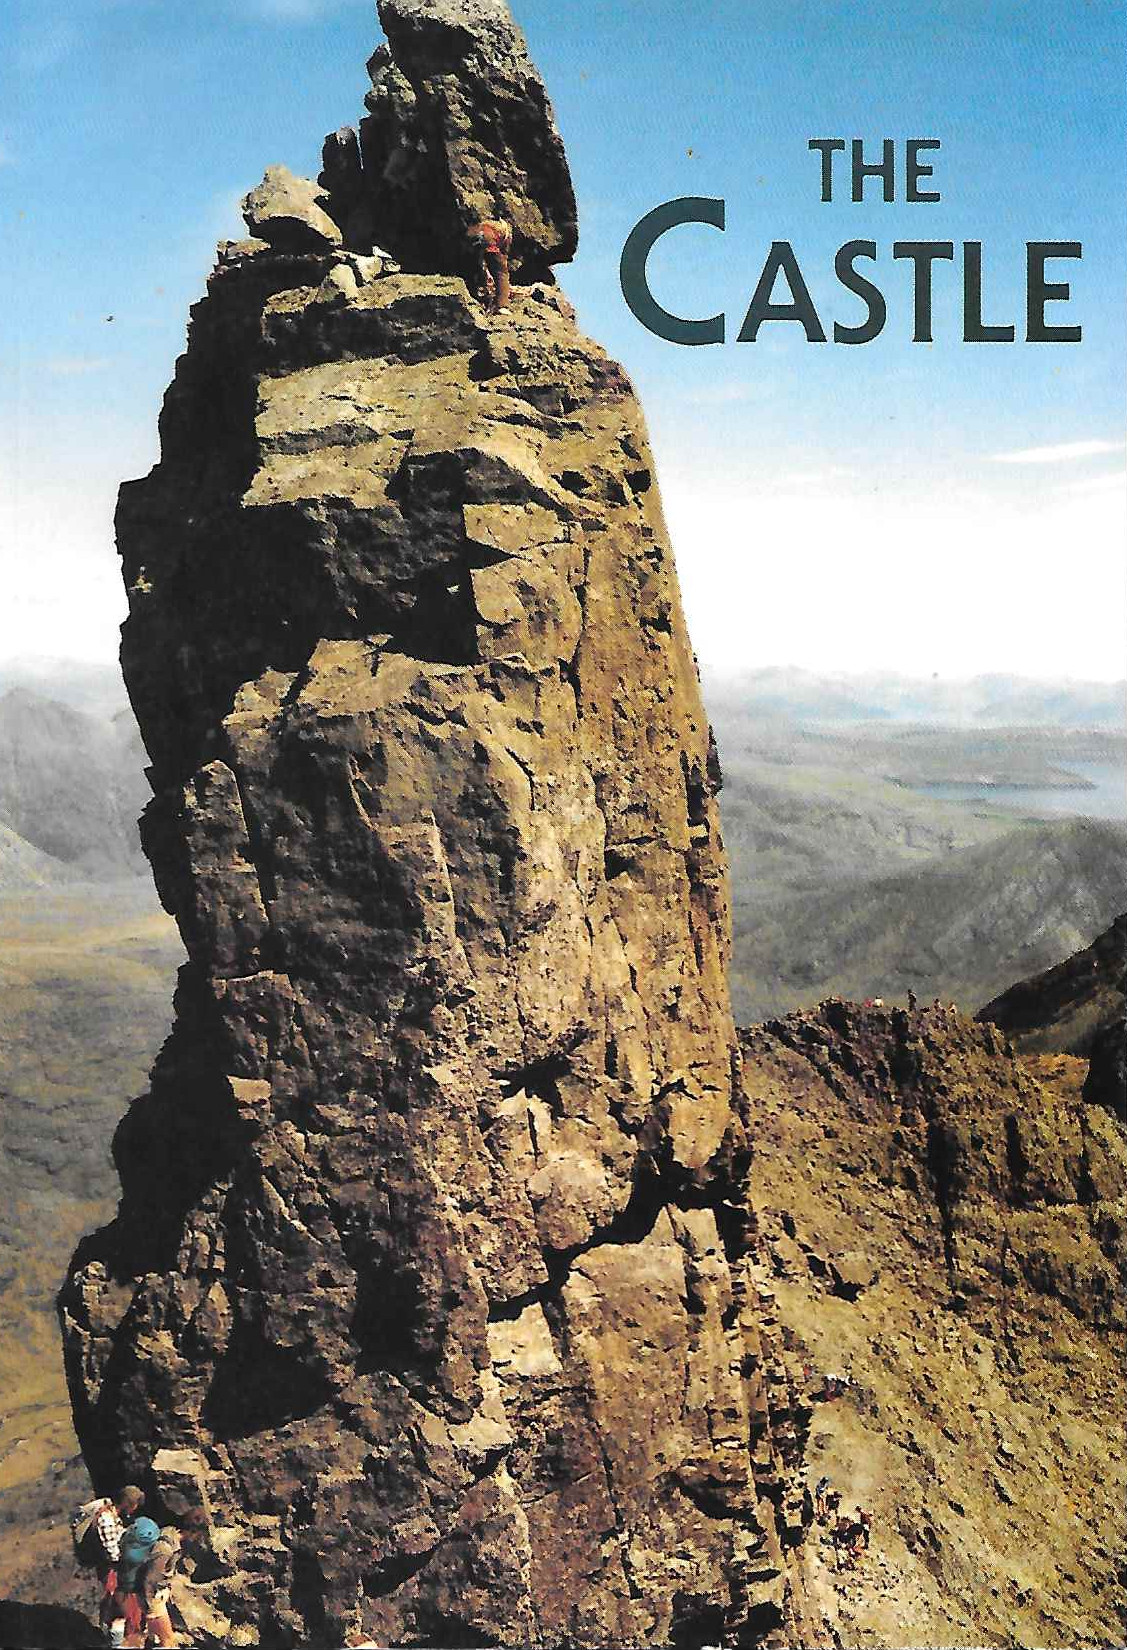
\includepdf{/home/ian/Documents/emacs/thecastle/images/frontcover.pdf}


\tableofcontents


\chapter{Foreword}
\label{sec:org81e3a1a}
\chapterauthor{Alf Gregory}
The chapters in this book will bring back many personal memories and
make us think of the great days we have spent in the hills, for most
of us have had mountain adventures we shall never forget. These might
be toiling up the final slopes of Mount Everest, battling against wind
and rain on Kinder Scout or leading a hard route on Lakeland rock.

There are times when it is sheer hell and we wonder why we are there
at all, but on other days it is so fantastically beautiful we realise
there can be no other way of life, for the joy of mountaineering is a
mixture of so many things.

Living close to the hills, as many of us do, is our greatest privilege
and we can sometimes feel sorry for people who do not have the good
fortune to share our glorious environment. However, the important
thing is to use this to the full, cherishing and enjoying all its
natural beauty, but at the same time accepting the challenge the
higher mountains offer, for in return they will give us unforgettable
days of adventure.

It is in the companionship of an organization like The Castle
Mountaineering Club that the mountain life can be enjoyed to the
full. The articles in this book prove that and show what a wonderful
twenty one years it has been for this Club. The next twenty one should
bring even more successful climbing and hill wandering.

\chapter{The Founding of the Club.}
\label{sec:orgc4ebc9c}
\author{by Mike Anderson}
Langdale, 29th September 1967: torrential rain, the road flooded in
several places, the campsite very much the same. Hardly an auspicious
first meet for a new Club, but one that is nevertheless still
flourishing twenty one years later. All members of the Club have since
experienced similar discomforts, with the additional attractions of
cold, hail, sleet and snow. Now at last we can reveal where the
responsibility lies.

Alec Barclay came from across the Border to seek satisfaction for
causes long gone: at least that is what we put it down to when we were
induced to go to Scotland and elsewhere to be tortured by long walks
and hard climbs. Alec and his colleague Colin Mackie had first taken a
small party of Sheffielders for a weekend in Glencoe in March 1967,
followed by a further visit in July the same year. It was after these
trips that the idea of forming a club came to Alec. Discussions back
in Sheffield met with enthusiasm and convinced Alec that he had the
nucleus for the formation of a viable club.

A nine strong meeting of stalwarts held at Ashley and Avril Turner's
house on Monday 25th September 1967 led directly to the founding of
the Club. As all of them were "regulars" at The Castle Inn at Bradway
it was natural and appropriate as they intended to meet there on their
weekly club night that the Inn should lend its name to the Club. But
what to call it? The Castle Climbing Club, or The Castle
Mountaineering Club? After a long discussion it was decided to name it
"The Castle Mountaineering Club", in the belief that this title
indicating the basic principle of putting one foot in front of the
other to gain height would provide the widest possible base for the
Club and give encouragement to prospective new members.

A proposal by Alec that the Club should exist to further the spirit of
mountaineering on the one hand and to offer instruction in specific
techniques on the other, was duly accepted. It was agreed that The
Castle Inn should be the Club's headquarters until suitable premises
could be found. Alec himself would act as first Hon. Secretary and
Colin Mackie as first President, a , committee was duly elected and a
constitution adopted on 9th October 1967.

The success of The Castle Mountaineering Club owes a great deal to the
decision taken in those early days to establish the Club as a
"Mountaineering Club". Members have been encouraged over the years to
extend their mountaineering skills over a wide range of activities, be
they climbing, hill walking, skiing or pot holing even pot holing: a
little difficult to put one foot in front of the other underground and
still gain height! Whatever the activity, the Club has always afforded
opportunities for its members to acquire experience in all aspects of
climbing and mountaineering.

Regular meets were held from the outset with climbing sessions every
week on local Edges and an away meet each month to different parts of
England, Wales and Scotland. The Club rapidly became something of a
family with meetings in members' houses and with slide shows and
lectures in addition to the regular club nights at The Castle Inn.

THE FIRST STEPS HAD BEEN SUCCESSFULLY TAKEN.

But with growing membership, the need to find a clubroom which would
fulfil one of The Castle's ambitions soon became apparent. That saga,
an epic in its own right, was about to begin.

\chapter{The Clubroom Project}
\label{sec:org06324ed}
\chapterauthor{by Mike Anderson}

It was in early July 1969, after two years of frustrating
and fruitless searching for a suitable clubroom, that Alec and
Colin were having lunch at The Rising Sun on Abbey Lane
Sheffield. Whilst discussing the Club with the licensee Ada
Bennett, they became aware of the dilapidated building behind the
Inn.

On examining the beautiful old building with its ivy covered
roof and fine stonework, it was immediately apparent that there
was great potential here in terms of the long awaited clubroom.
Interest was declared and Ada, although in favour of the
proposition, made it clear that the final decision must rest with
the Brewery and that they would need to get in touch with the
Brewery Manager.

Fortunately, our friend Mike Collins was not only the
Brewery Manager but also a "regular" at The Castle Inn where the
Club was then still meeting. He immediately took up our cause and
his enthusiasm for the project was boundless. In August 1969,
Alec had talks at The Rising Sun with a local Director of the
Brewery and members of his works department.

It was originally intended to occupy only the top half of
the building which was formerly a corn and hay loft, but on
closer inspection the upper floor joists and floor boards were
found to be riddled with woodworm and would need to be entirely
replaced: even the external doors were hanging off their hinges.
After a quick inspection the parties were glad to retire to the
more congenial surroundings of the bar of The Rising Sun to
discuss the matter further.

Now Alec had always been a talkative type of person  the
less kind might call it verbal diarrhoea  but on this occasion
this characteristic proved an invaluable asset. Alec could not or
would not stop talking, the Director needed to get back to work
and in order to get away felt obliged to promise that the Brewery
would strip out the whole of the interior of the building and
make the property structurally sound. It was agreed by Ada that
the Club could then rent the premises at a nominal figure. By the
end of September 1969, the Brewery work had been completed and
the building was available for our use.

It was at this crucial juncture that Alec presented himself
at Mike Jackson's office and asked him if he would like to be
Hon. Secretary. Mike said "No!"  Alec, it appeared, had to move
back to Scotland for business reasons and therefore unfortunately
would not be able either to continue as Hon. Secretary or take
part in the building of the clubroom. It has long been rumoured
 and believed by the very best of his friends  that Alec had
asked for a transfer back north because he had guessed what might
be in store. He asked Mike again, praising his powers of
organisation, his loyalty and the need for a steady hand on the
tiller. Mike again said "No!"   even more definitely. The verbal
diarrhoea flowed and Mike just did not stand a chance. A new Hon.
Secretary was in the making.

Our initial aspirations for the clubroom were limited to a
casual use of the existing building, although we had vague hopes
that we might be able to use one gable end as a makeshift
climbing wall. We planned to utilise our camping equipment to
provide heat and light and simply to install a few items of
second hand furniture to be donated by the Brewery. During a
visit to collect benches and stools, we noticed that the staff
were taking up the old cobbled brewery courtyard which over the
generations had been tarred in place to take the weight of horse
drawn drays. This was an opportunity too good to miss and as the
cobbles came up they were delivered to the yard of The Rising
Sun. But the mass of filthy black stone grew to alarming
proportions and it was painfully obvious that a good many
generations of horses had passed over them and left their
deposits in more ways than one.

Now the Club was fortunate in having an architect in its
ranks in the form of Kerry Brooksbank and Kerry had kindly
offered to give us a hand. On our very first day of work we
gathered in the pub yard to be greeted by a huge pile of
exceedingly evil smelling tar and horse encrusted cobbles. We
were under the impression that all we were going to do was to
clean them up as best we could and stack them into place. How
could we have been so gullible?

Looking first at the cobbles and then at us, Kerry picked
one up. It was shaped somewhat like a loaf of bread, rounded at
the top and tapered on both sides. The wearing face had been
slightly fractured by horseshoes and wagon wheels. He turned the
stone over and to our surprise, struck it sharply with his
hammer.

With a cry of "That's it!" he stood there grinning.

"That's what?" we responded in unison.

"We face it."

"We what?"

"We chisel a face on every stone."

"Every stone?"

"Every one!"

What was the man talking about? He must be joking  or had he
just taken leave of his senses? Face it? All of it? Just thinking
about it almost made us walk off and leave him standing there. He
couldn't mean it: sentenced to hard labour and rock breaking
without trial. Our hobby was mountaineering, not serving time. He
couldn't be serious\ldots{} but he was. Every single stone was to be
cut to reveal the beautiful lines and colours beneath the grime.
All twenty tons of them.

Kerry immediately undertook to prepare detailed drawings for
a stone built clubroom and then to supervise all the building
work that would be entailed, essential if the enthusiasm of
members without any building experience whatsoever was to result
in a finished product worthy of themselves and the Club. Even
then, little did we realise just what Kerry had in mind and the
magnitude of the task we were about to undertake. It was not
until he presented us with a line drawing that the full extent of
his ambitions dawned on us.

His basic plan was to convert half the ground floor of the
building into a "snug" with a room above in which to store Club
equipment. His scheme called for a raised floor for the snug room
and a massive stone centre column with embedded flagstone steps
forming a staircase to the upper floor. The inside walls were to
be stripped back to the original stonework and the ceiling of the
snug was to be of new timber supported by two substantial beams,
all the woodwork to be varnished to enhance its appearance. A
fitted bookcase would not only house books, maps and climbing
guides but also separate the snug from a small galley  bench
seating, carpets and spotlights would finish the project. ,
Having decided what to do, it only remained to do it, easier
said than done. Where were the funds, materials and labour to
come from? The last was easily solved as Club members would of
necessity have to undertake the work themselves, but financing
the project would be  more difficult with the subscription only
 1 a year. As for materials, we already had our building stone
but a great deal more material would clearly be required and so
the scrounging began.

A friendly builder gave us permission to "cannibalise" an
old bungalow about to be demolished and one evening the
equivalent of a plague of locusts descended on the unfortunate
property. Under Kerry's direction, floors and quarry tiles came
up, joists came out, many a mile of electric wire was gathered
and the lead on the roof  already being eyed by local citizens
was stripped off. The entire booty was loaded in an assortment of
vehicles and the convoy set off for home well after dark. Kerry
brought back all the lead in a borrowed Land Rover, laden to the
wheel arches. Dressed in his glad rags, covered in dust and
without any form of identification, he could hardly be expected
even to remember the registration number. It seemed to us a shame
that he was not pulled up by the local Bobby. "You won't believe
this, Officer \ldots{}"

Over the coming months many members came to lend a hand, but
the dedicated hard core were to be seen on site several evenings
a week and most weekends. The major task involved cutting the
stone, mixing cement and building the central column with its
flagstone steps. The stone was so very hard that several blows
were required to achieve even one cut on the face of each cobble
but as we gradually grew more expert it became a joy to work
with, such was its superb quality.

You could always tell our stone masons by the large painful
bruises on their hands, the strained wrists and the blood stained
finger bandages where the hammer had missed the chisel. To cover
our embarrassment, we claimed that the injuries were hand jamming
scars! We soon became adept at technical jargon and spoke
knowingly but incomprehensibly of corbels, coigns, jumpers,
gobbo, compo and lump hammers. Our world revolved around the
four to one mix. Our shoes were disgusting, our finger nails were
full of cement and our hair varied from grey to white to brown to
grey as the dust and cement flew around. -

Throughout the building programme, every single bag of sand
and cement had to be purchased and  brought on site, water was
obtained by the bucket from Ada's outhouse and lighting was by a
single lamp. When it got too dark you went home. All cement had
to be mixed by hand and all stones first cut to size and then
laid to plan. After every building session, a return visit was
required in order to brush out the mortar joints and create a
marvellous three dimensional effect.

The hundred year old ivy, previously allowed to go its own
way, covered the entire roof and gave us a different type of
problem as it was growing through the stone roof tiles and
hanging down on the inside from the ceiling to the floor. The
ancient stems were so closely entwined that the mass of
vegetation had to be laboriously cut out in small pieces, so as
not to dislodge the tiles. This was very tough work indeed and
two particularly intricate pieces were preserved in order to
display them in the clubroom fireplace.

After a daily visit over a period of several weeks to a
church under demolition, we salvaged several carved feature
stones which were sand blasted and used to support the two main
beams supplied by our friendly builder. The doors and all the
window frames were taken out and replaced, the plumbing installed
and the entire building rewired to modern standards.

Saturdays, Sundays, club nights and any spare time went into
building work and slowly, very slowly, the project began to take
shape and to resemble the plan. We felt that we were now becoming
very professional and Kerry must have thought so too, for as the
work progressed and then neared its completion, he kept coming up
with another wall to be built or a corner to be faced with stone
and even a decorative archway.

All in all it was a very busy time but like all things it
thankfully came to an end. With the snug floor laid, the centre
column built, the galley completed and the upper floor in place,
all that remained was to provide the finishing touches. Kate Peek
hand carved an archway stone dated 1970 whilst Bryan Metcalf
created a copper Castle motif with crossed ice axes to decorate
the snug fireplace. Tables, benches and chairs had been provided
by the Brewery and the carpets, together with books, maps,
pictures and photographs, were donated by members to make the
clubroom all the more comfortable and welcoming. -
The entire building programme in all its variety and
complexity was carried out by our own enthusiastic and willing
Club members, albeit under Kerry's expert guidance. The standard
achieved with little or no previous experience in building no
doubt surprised even the members themselves. Starting from
Kerry's basic concept, the carrying out of the entire project has
proved so successful that no substantial alterations have been
required over the years and the clubroom today is as fine and as
practical as ever.

However, at that time the mountaineering enthusiasts had not
fully taken into account the doubts of a number of Castle Inn
"regulars" who could not bring themselves to accept the move from
their beloved watering hole. Even after an impassioned plea from
Alec in Scotland, the move was sanctioned by the committee only
on the casting vote of the President, a remarkable performance in
the light of the magnitude of the task already undertaken and
completed.

We were now committed irrevocably to the future of the Club
and its new clubroom which we intended to use as a springboard
for our outdoor activities. But could it be viable without the
support of those early members who had stayed at The Castle Inn?
It was a question we were to ask ourselves many times over, as on
our first club night at the clubroom, a grand total of eight
turned up. Thankfully, the enthusiasm of the loyal climbing and
hill walking members prevailed and as the advantages of having
our own clubroom and meeting place became more and more apparent,
so the membership again began to grow with a welcome influx of
keen climbers and hill walkers. On 21st April 1971 a grand
opening party was held when Sir Jack Longland officially opened
the clubroom and paid tribute to the hard work and achievement of
the members.

By now we were all not only climbing and walking the hills
at every opportunity but also starting families, building careers
and setting up businesses. Nevertheless, after only a year the
stalwarts began to get itchy fingers and to prepare plans for the
erection of a climbing wall on the inside of the empty gable end
a climbing wall to give members an opportunity to fill those dark
winter nights. We learned that two cottages were being demolished
and after negotiating for the stone, we organized a number of
lorries and a further twenty tons of large sandstone blocks were
loaded and delivered to the clubroom in one day.

WE WERE OFF AGAIN!

It was a peaceful Sunday morning when the first lorry
arrived to be unloaded by members. At first the stone was neatly
stacked, but the sheer volume soon overcame our efforts. The pile
grew higher and higher until it topped the boundary wall, itself
seven feet high, by some three feet. But the fully laden lorries
kept arriving.

At the height of this activity, Ada  who had in fairness to
the Hon. Secretary had been warned that "a few stones" might be
arriving  sallied forth to express her heartfelt indignation. As
she came into the yard, a very large lorry was noisily attempting
to extricate itself from the huge mass of stone in front and the
ever growing pile it was tipping behind. The  din and the clouds
of diesel fumes were absolutely appalling. The Hon. Secretary
 remember, he's the one who got talked into this job  looked
round for moral support from the loyal members busily working at
his side. He needn't have bothered: not one was to be seen and
Ada's considerable wrath descended on him unabated and at great
length. Mike is not very often lost for words but it would have
been easier for him to dam the Grand Canyon than to put up any
resistance. He listened, tried to look intelligent and said very
little, a ploy he had already tried out unsuccessfully on Alec.
Guilty as charged!

The stone masons were brought out of their happy retirement
and the building work began again. The climbing wall progressed
quickly, as it proved much easier working indoors with power and
water laid on.  Great attention was given to detail, with
undercut holds, hand jamming cracks and overhangs constructed to
the precise requirements of the climbers. The design incorporated
an open fireplace with a flue inside the wall, mischievously
described as the one and only centrally heated climbing wall! The
fireplace itself also serves to provide a genuine mantle shelf
start to the main face.

One last area remaining for improvement was the main
entrance. A canopy was built, stone flags laid and a stone
grinding wheel erected to provide a decorative finishing touch
with local interest, this being of course The Peak District ,
 National Park emblem. Kate, as artistic as ever, carved out a
second stone, this time dated 1972.

APRIL 26TH 1972   FINISHED!

No more stone to cut, no more fittings to fit, no more
mixing of cement and no more painting. Party time with a firkin
of ale, a whole range of goodies made by wives and girlfriends, a
time to celebrate. Sir Jack Longland came back to do the honours
and we were joined in our celebrations by representatives of the
Brewery, members of other climbing clubs, the Press and all who
had made our clubroom possible. The night was long and one to
remember.

Since then, members have been involved in the promotion of a
film in Sheffield depicting the local climbing scene and the
premiere of "Whillans on Everest" in 1971, a scoop for the Club
and, even if something of a gamble, a means of meeting our
building costs. They have taken an active part in the formation
of the Sheffield Association of Climbing Clubs  SACC  and have
extended a helping hand to many, including the hard lads from
London's East End who met their match on the local gritstone
Edges. Most of all it has been fun and our clubroom provides
unique and welcoming surroundings in which the members and their
friends can enjoy each other's company and plan their outdoor
activities.

Throughout the years, the Club has certainly seen many
changes in climbing techniques, from the early days when we filed
the threads out of nuts, to the high tech "Friends" of today. It
is not unusual these days to see a pair of bright pink tights on
the climbing wall on a club night, enhancing the style of their
proud owner. Progress, it would appear, comes in many forms. Even
the Club's newsletter is computerised: now there's progress!

Members can be found visiting all parts of the world ranging
from the Himalaya to the Antarctic, from South America to Africa
and from the Rockies to the Alps   a far cry from those early
days when each away meet was an adventure in itself and a meet in
Scotland the limit of our ambitions. With Alec starting a second
Castle Mountaineering Club in Edinburgh   yes, he's at it again!
  it only remains for Kerry  who moved to Johannesburg  and for
Kate and Alan  who moved to Norway  to do the same and we shall
truly enjoy worldwide connections. ,
Throughout the first twenty one years of its existence the
Castle has enjoyed the services of outstanding Club Officers who
have taken a full and active part in organising meets and
encouraging members new and old, ensuring the smooth running and
progress of the Club. The friendship and companionship of The
Castle Mountaineering Club are very special and just as members
have given their best efforts to the Club, so the Club has
brought together many people from different walks of life to
share the joys of climbing the crags and tackling the mountains.

The foundations of The Castle Mountaineering Club have been
well laid and with its unique features and the enthusiasm of its
members, its future is clearly secure.

\begin{figure}[htb]
\centering
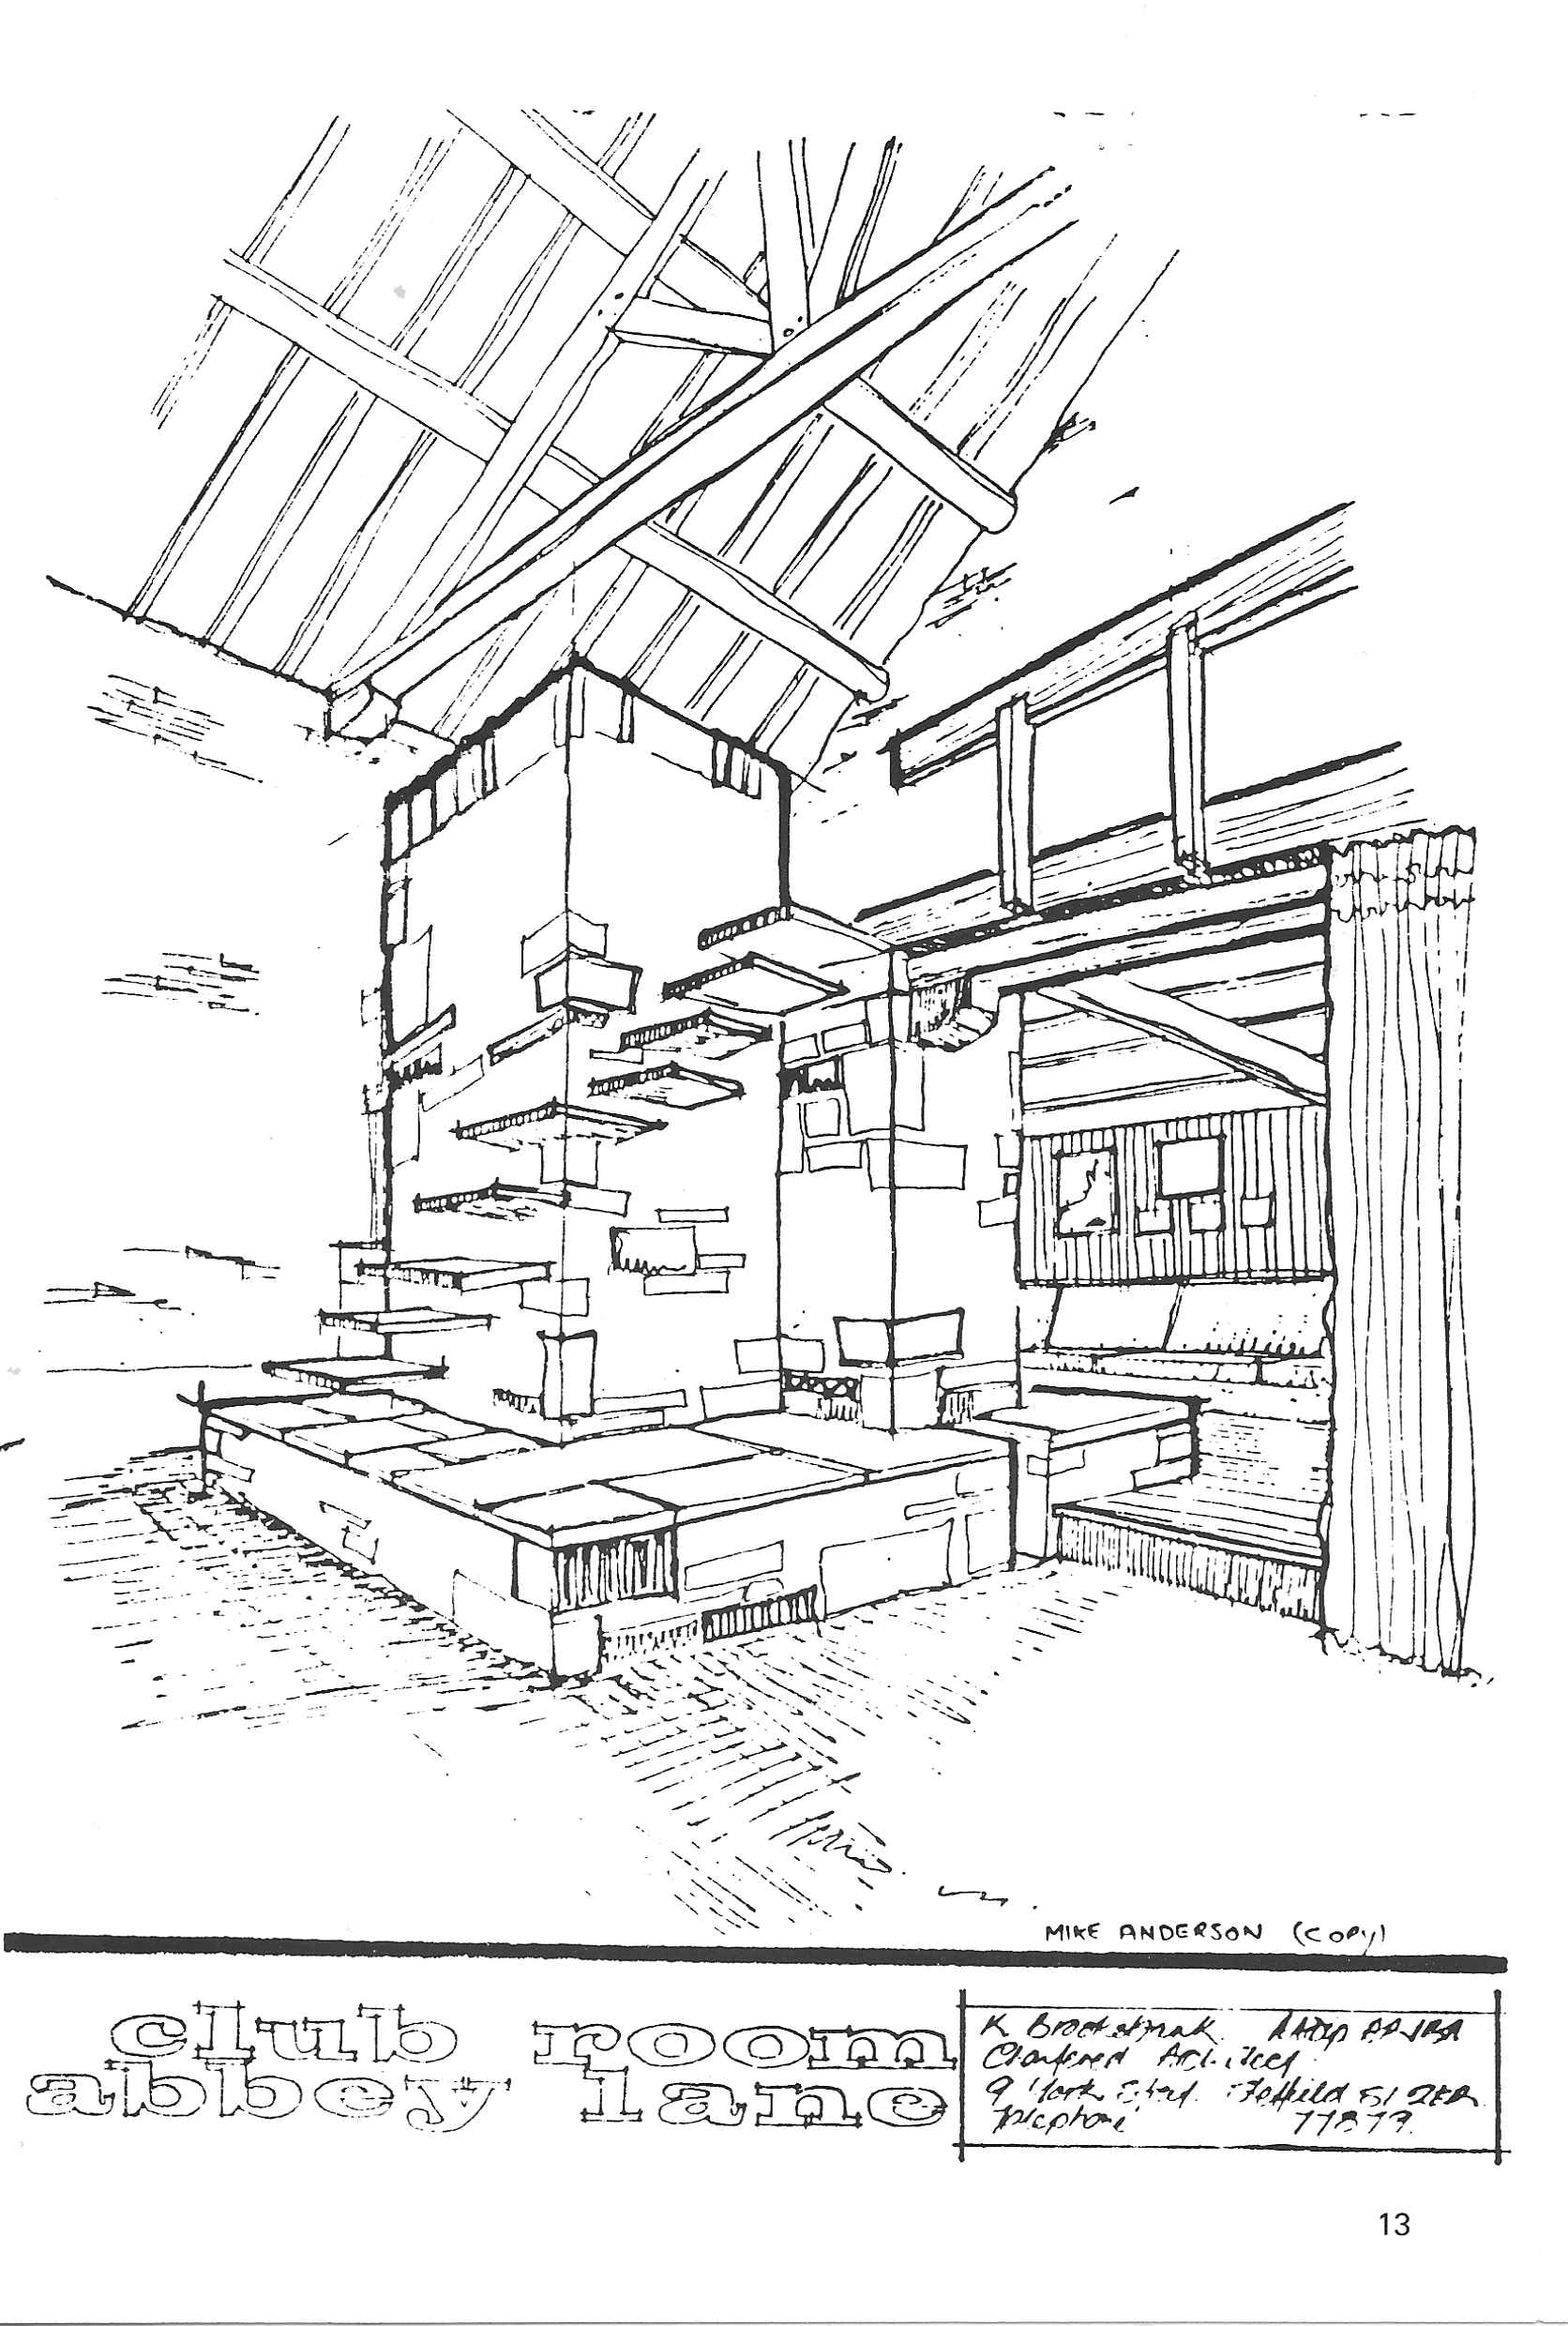
\includegraphics[width=.9\linewidth]{./images/Plan1.jpg}
\caption{\label{fig:org794a21d}
The Clubroom and Climbing Wall.}
\end{figure}

\begin{figure}[htb]
\centering
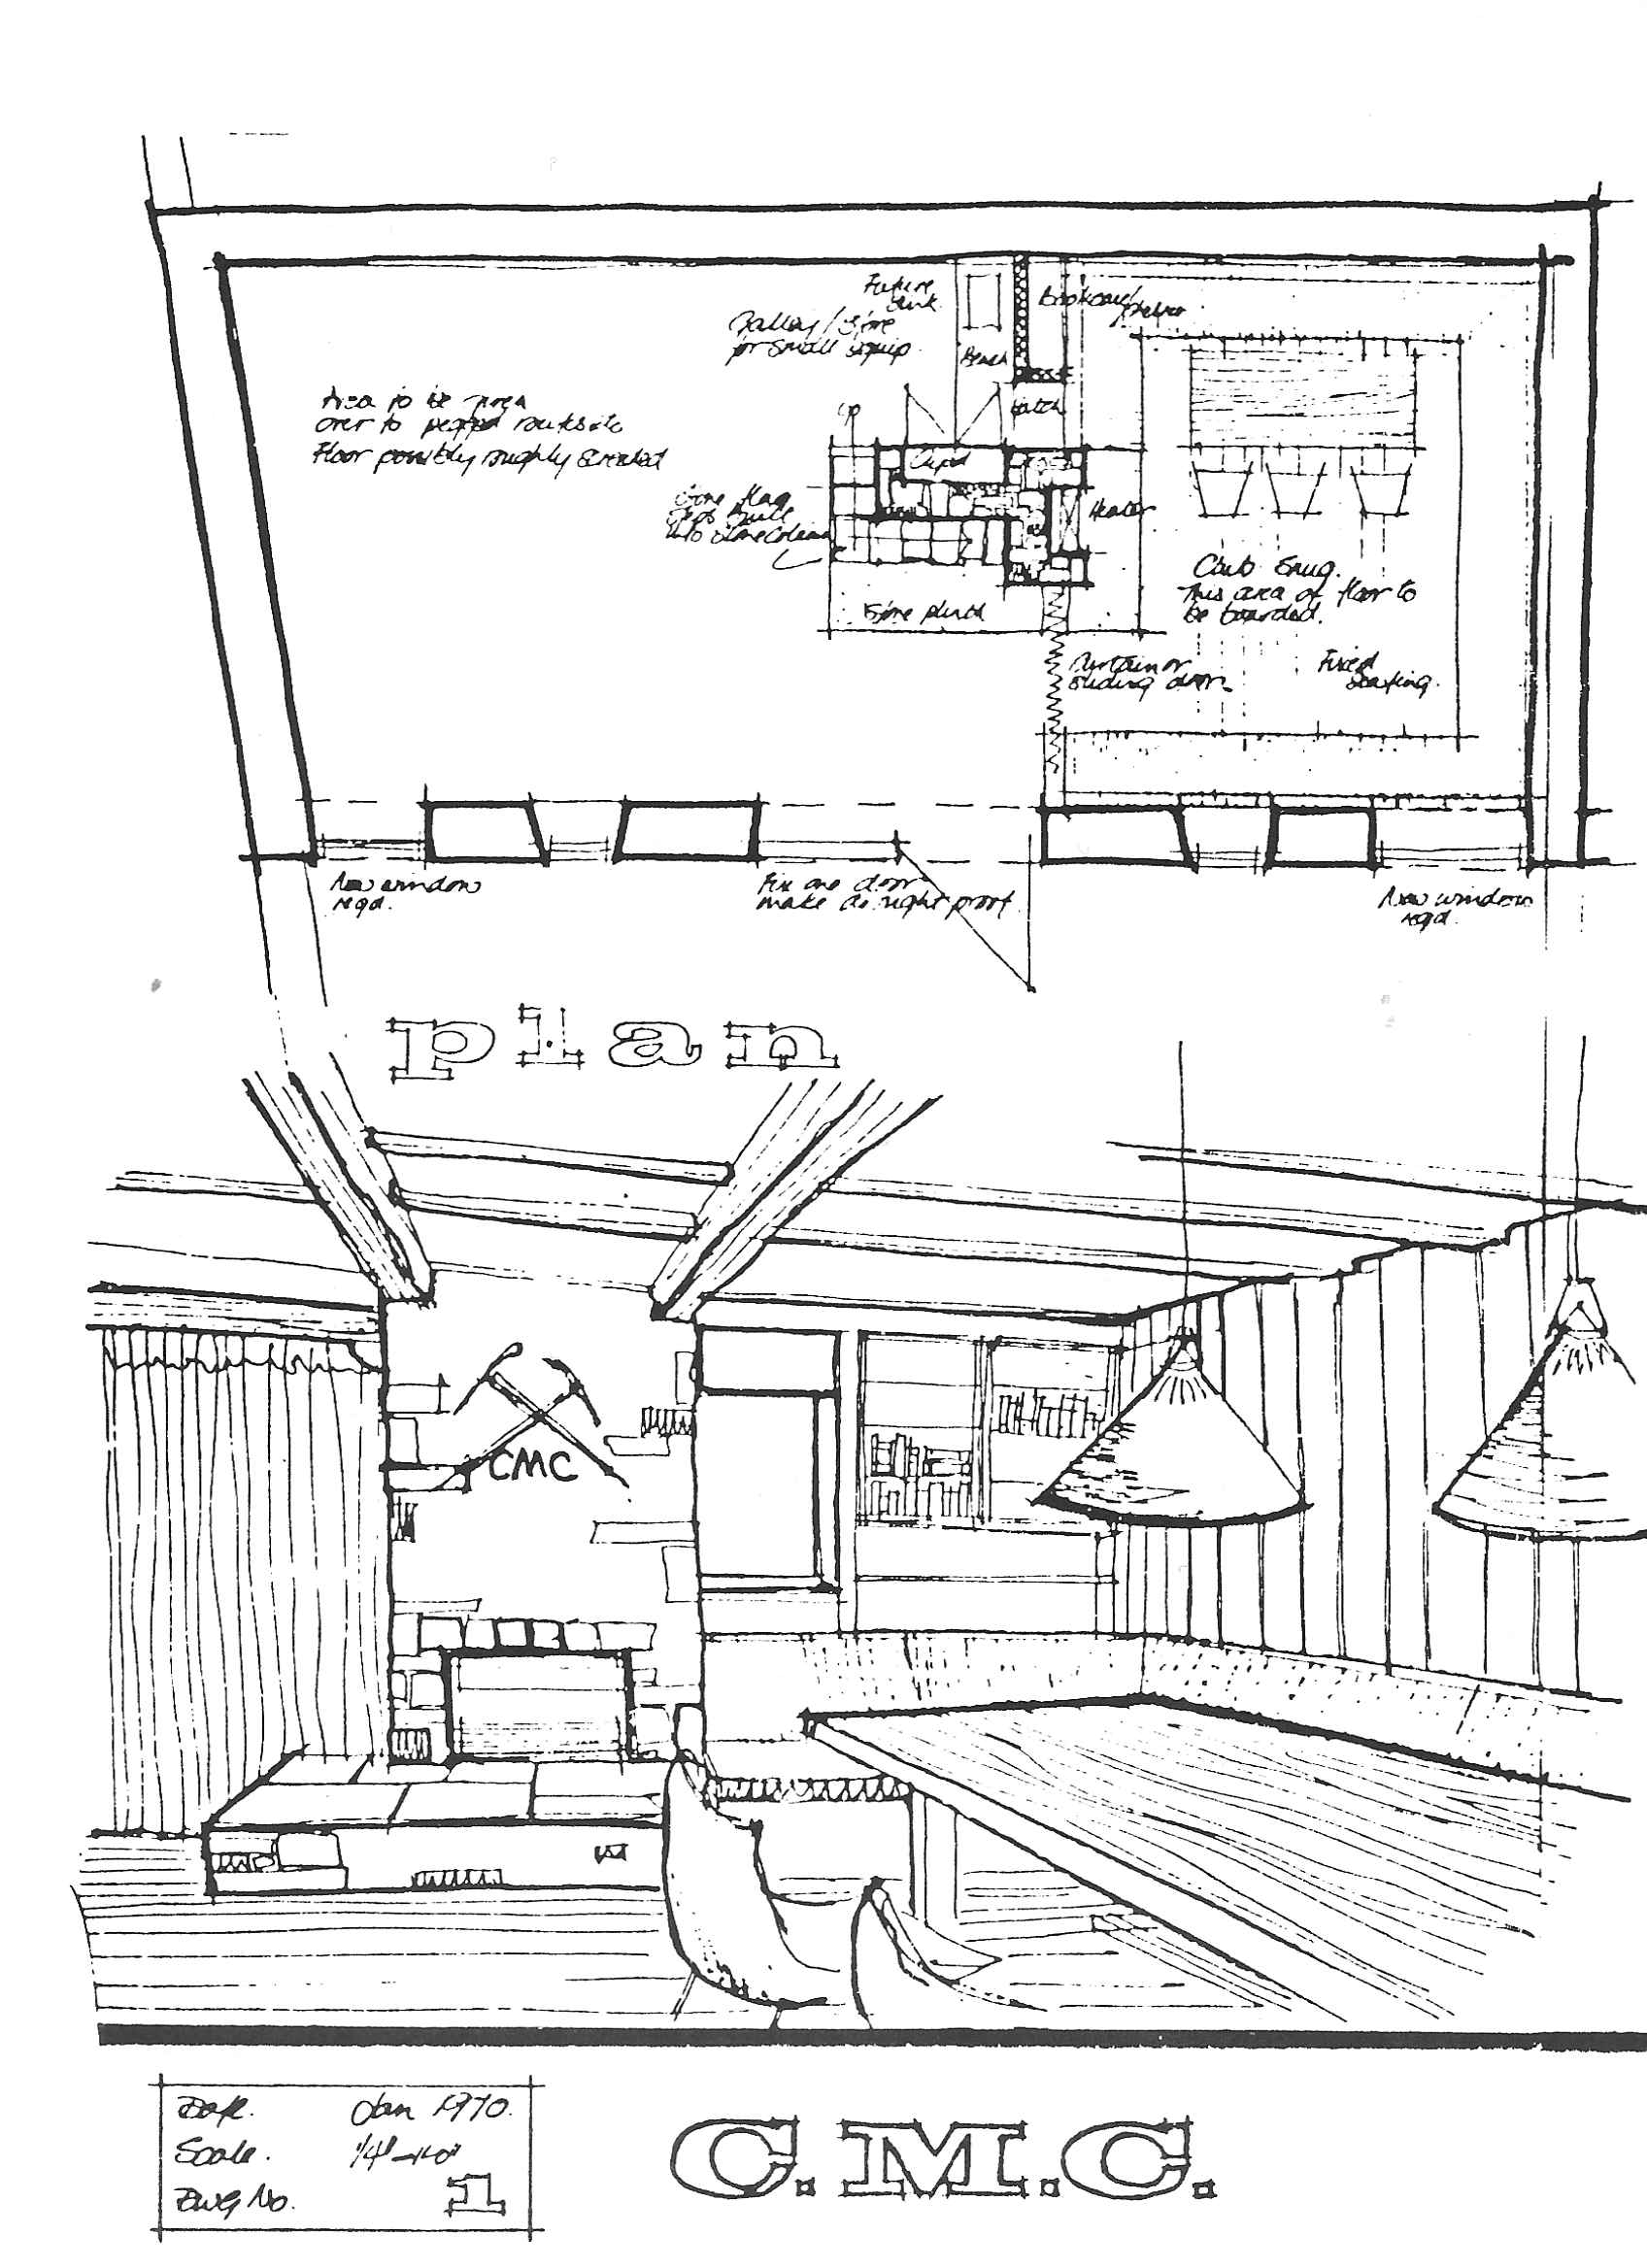
\includegraphics[width=.9\linewidth]{./images/Plan2.jpg}
\caption{\label{fig:org4ac23ed}
The Clubroom.}
\end{figure}

\begin{figure}[htb]
\centering
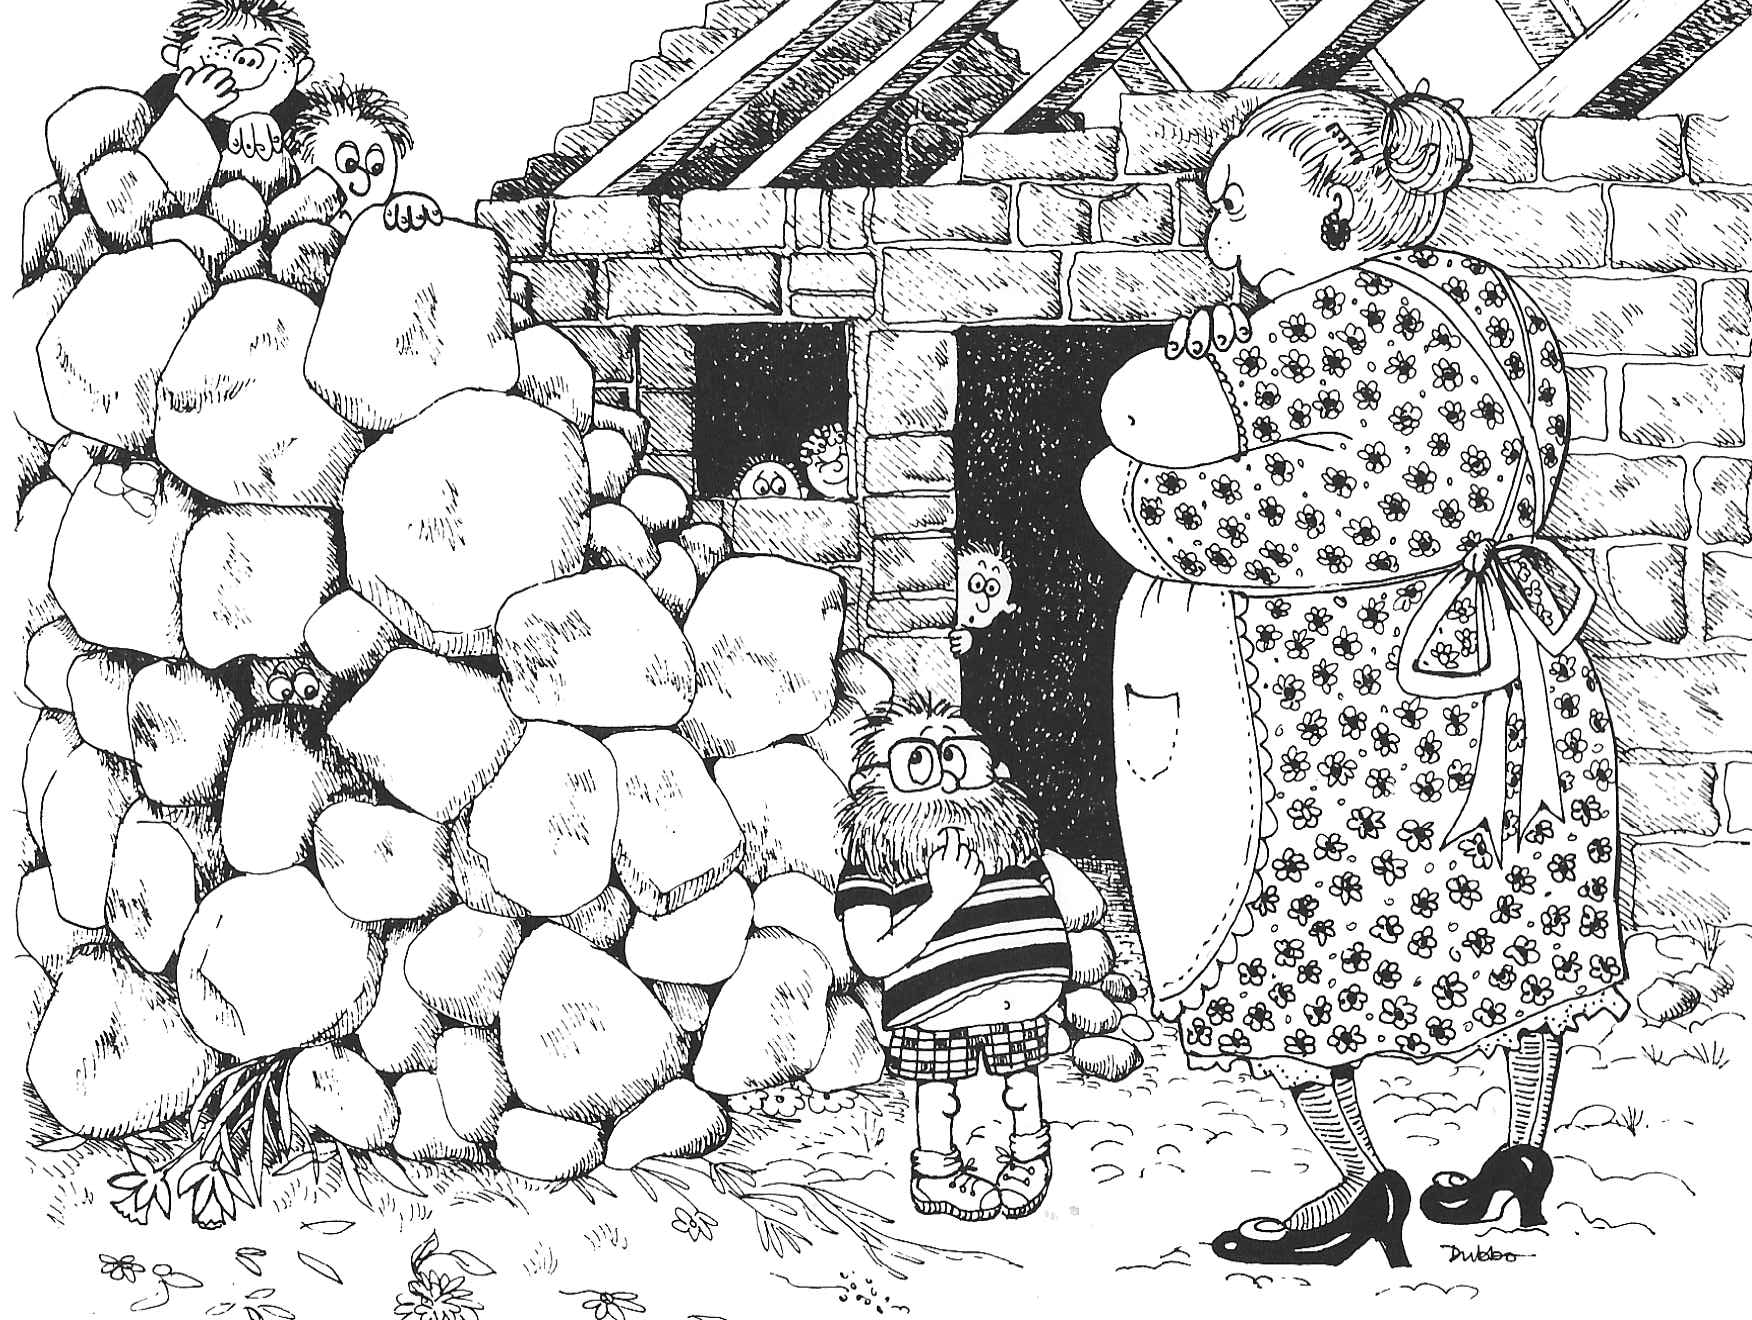
\includegraphics[width=.9\linewidth]{./images/Cartoon_01.jpg}
\caption{\label{fig:org37f0ef9}
Renovating the Clubroom.}
\end{figure}

\chapter{Cairngorm Plateau Traverse}
\label{sec:orged356d4}
\chapterauthor{by Mike Jackson}

\begin{figure}[htb]
\centering
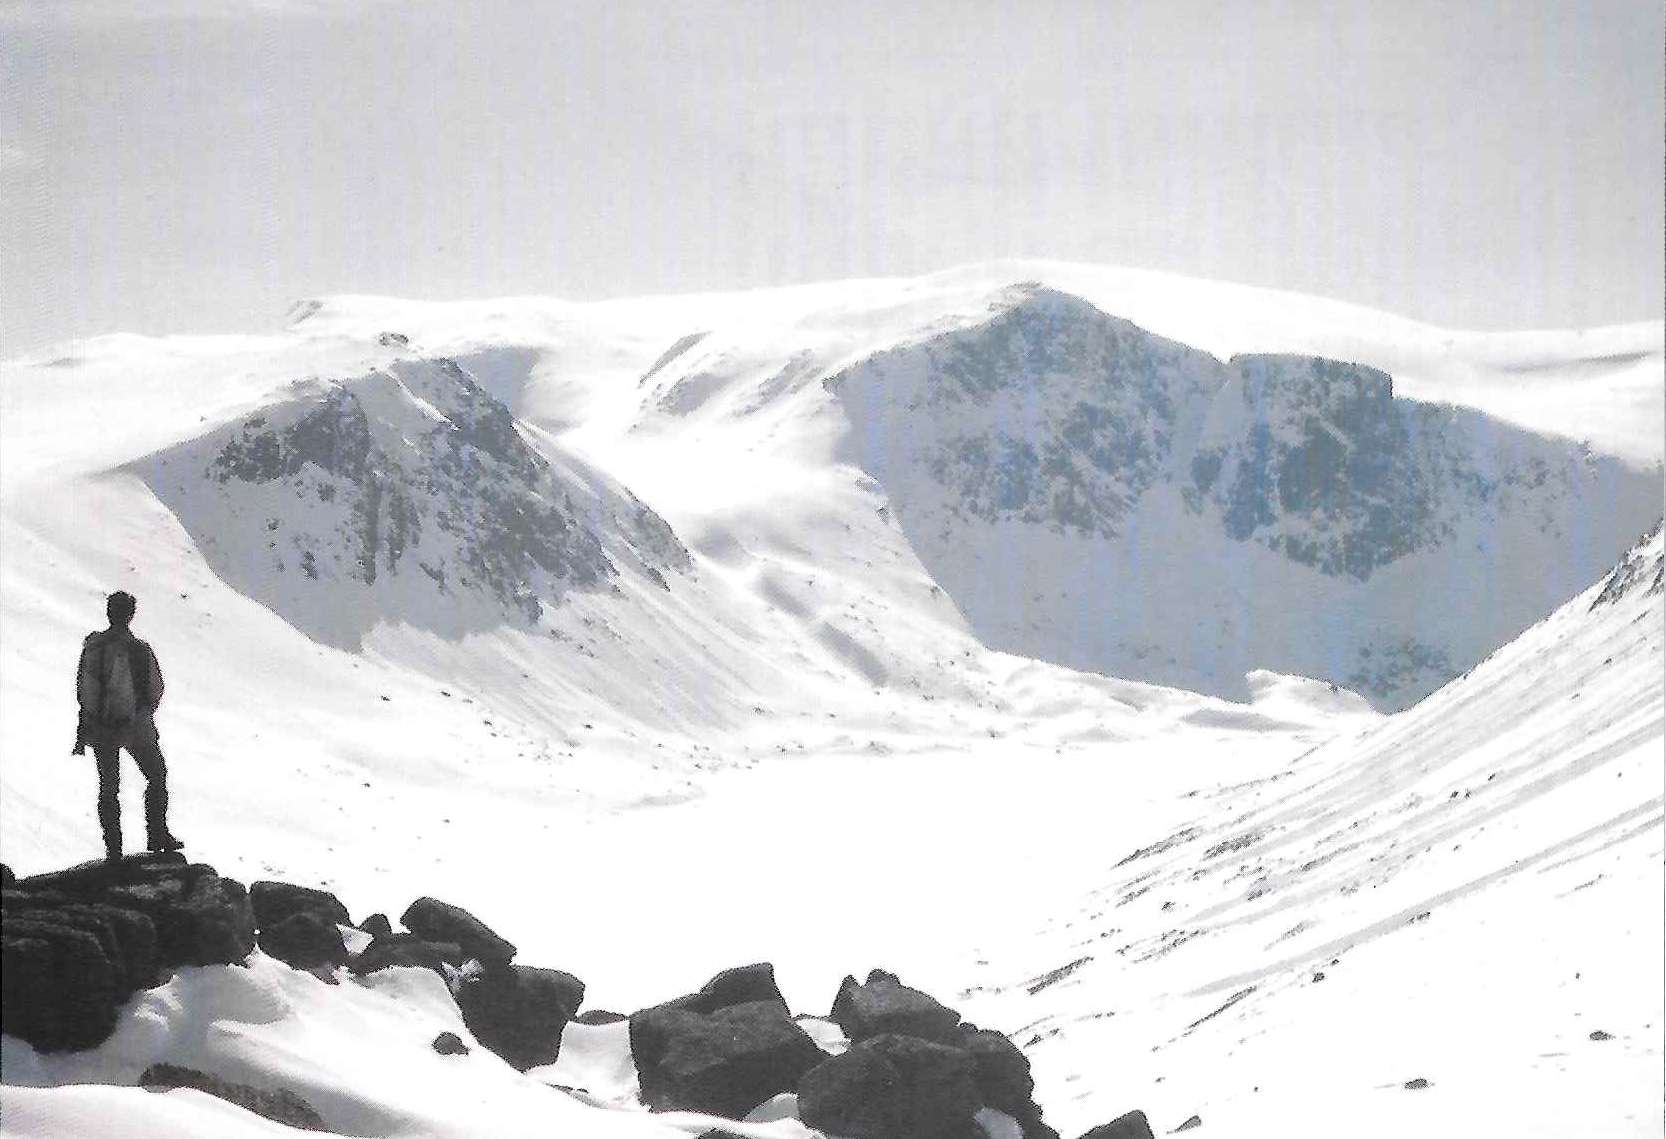
\includegraphics[width=.9\linewidth]{./images/Ben_Macdui.jpg}
\caption{\label{fig:org4d39097}
Ben Macdui Beyond Loch Avon (Frank Mellor)}
\end{figure}

An annual highlight in the early days of the CMC was the
winter visit to the Cairngorms. For many members this was their
first experience of the magnificent snowscapes and near arctic
conditions to be enjoyed  or endured  in Scotland during the
winter months. A particular outing on these hills in February
1970 proved to be one  of the outstanding days of an early CMC
Cairngorm Meet and at the same time illustrates very well the
conditions one may reasonably expect to meet in winter in the
Highlands. Our party consisted of Mike Anderson, Jack Ashcroft,
Chris Taylor, Paul Goodlad, Dick Arnold and myself and our
objective was to traverse the great plateau from Cairngorm to Ben
Macdui and back.

The early morning was beautifully clear under a blue sky and
with deep snow everywhere. I regret to record that certain
members were aided in varying degrees by the chairlift in their
initial ascent of Cairngorm. I myself had to endure an
uncomfortable "stitch" but the glorious views were ample
compensation. As we descended to the west from the summit, we
could pick out a column of walkers on the plateau below,
resembling a trail of ants and giving a wonderful sense of scale
to the scene. The vista ahead of Cairn Toul, Braeriach and Sgoran
Dubh Mor was particularly splendid and there was a magnificent
view across to Fiacaill Ridge and the neighbouring cliffs
plastered in brilliant white snow with huge cornices. The going
was fairly arduous as the snow was not sufficiently frozen to
take our weight and we were constantly sinking in up to our knees
and beyond. We made our way to the Corran Bothy near Feith Buidhe
 a bothy later demolished following a tragedy hereabouts when a
number of children perished in the snows  only to find it
completely covered by snowdrifts except for the yellow chimney
cowl which stuck out grotesquely from the snow. There was a
really breathtaking view across to Braeriach with its great
coires gouged out of the plateau, all completely snow covered
under a cloudless pale blue sky. The summit of Ben Macdui gave
further wonderful views, particularly across to Cairn Toul and
the peaks beyond it, down to Carn a'Mhaim and the great snow
filled trench of the Dee and far away to Beinn a'Ghlo well to the
south. The Devil's Point, a spectacular peak when seen from the
Lairig Ghru track coming in from the south, appeared far below
our elevated position as a minor protuberance in this great
winter landscape.

It was then that my personal troubles really started as I
became very ill and had to retire urgently behind snow covered
boulders. The "stitch" which had afflicted me most of the way to
Macdui suddenly became much worse and on the return journey it
was impossible for me to walk any distance without stopping for
breath. To make matters worse, the wind began to increase and
great black clouds were approaching from the north west. The
weather closed in rapidly and the spindrift, combined with
falling snow in the mist, soon created near "white out"
conditions. Before long I was reduced to walking a few yards at a
time and later on I was able to think only as far as the next
step in the deep snow. Most of the party had gone ahead but
fortunately for me, Paul and Dick stayed behind and were able to
give much needed assistance. I had never before felt so weak and
ill on any mountain trip and I was deeply and genuinely grateful
to my good friends for their assistance  without them, my
predicament would have been very serious indeed. The last small
ascent to the top of Fiacaill a'Choire Chais seemed never ending,
but we could at last descend the ridge, suddenly emerging from
the mist and snow to look down on a hive of activity on the ski
slopes below. Within a few yards the howling winds and generally
adverse conditions on the plateau had been left behind and  after
descending only a few hundred feet it was impossible to imagine
the violence of the wind and lashing snow which had made our
return so difficult. It remained only for us to stagger down to
the ski lift and safety.

All walkers undertaking this traverse would do well to bear
in mind the remoteness of Ben Macdui  even in these days of
chairlifts on Cairngorm  and the sudden changes of weather often
experienced in these great hills. I have never forgotten the
great contrast between our glorious sunny walk to Ben Macdui in
such wonderfully clear conditions and that return journey on
which my personal discomforts and the adverse weather conditions
combined to create a real nightmare. The views we had enjoyed
throughout the morning of these great snow covered mountains had
been outstanding under a clear winter blue sky, but the day ended
with gales, spindrift, dense mist and snowfall   a combination of
the elements among the most difficult and dangerous we learn to
face on our beautiful yet challenging mountains.

\chapter{The Ascent of CMC Slab or Fighting off the Poachers}
\label{sec:orgebfc557}
\chapterauthor{Alan Fowler}


In the Derwent Area guide, tucked in amongst the extremes on Froggatt
Edge, is a climb with the name CMC Slab . Yes, it's named after your
very own Castle Mountaineering Club. It came into being in the dim and
distant past when Froggatt was considered "worked out" and people
hadn't heard of Heartless Hare or Hairless Heart or any of the other
more recent weirdly named routes a time when cavemen lived and people
didn't use chalk or wear pink tights, when one could go out with 120
feet of number four climbing rope, two runners and the old Sheffield
Froggatt guide and be ready to climb anything in sight as long as it
wasn't above Severe . "What's that", you say? "Nostalgia isn't what it
used to be?" You could be right there.

What was I talking about? Oh yes, CMC Slab . It started as an idea
from Mike Parkin. For those who can't remember Mike he was over six
feet tall with an incredibly long reach. He could nearly out reach me
but then I'm only five foot eighteen. He liked delicate slab climbs
and he had recognised the possibilities offered by the slabs between
existing routes on Froggatt. He was due to take a new job in North
Yorkshire and wanted to have an attempt at the slab left of Heather
Wall before he moved on.  Knowing how secretive one must be about new
climbs, he asked me if I could go with him to look at it one evening
when it would be quiet. But the summer went by and we somehow didn't
get the chance, so just before he had to leave, we went to Froggatt on
a Sunday.

We had a close look at the slab and it looked possible, if a little
green. I abseiled down with a wire brush and cleaned everything which
looked vaguely like a hold. Predictably, word rapidly spread along the
Edge and before you could say "EB" a crowd had gathered.

I top roped Mike and after a couple of attempts he managed the awkward
bulge above the ledge without using holds which could properly be said
to belong to Heather Wall . The slab above went well but before he
could descend to attempt leading the new climb, another couple had
roped up and were already on our route.  Our route! A short pause to
allow the booing and hissing to subside.

The leader put a runner in Heather Wall and managed the bulge. Mike
was at the bottom to fight off other interpolators whilst I stayed at
the top ready to throw sand down the route if this scoundrel looked
remotely like managing the top slab. I needn't have worried. In
attempting to reach the finishing pockets his feet slipped, resulting
in a satisfying pendulum into the right wall of the corner. Another
attempt ended the same way and after a few encouraging words from me
like "You'll never make it I should pack up and go home" and "Come
back when you're feeling on form" he decided that his right shoulder
couldn't take any more and he did in fact pack up. Mike then took his
chance to lead the climb in fine style and I seconded.

Thus CMC Slab entered the history books as "A rather artificial climb
using the stances and protection of Heather Wall ". I see that they've
squeezed another route in further left.  It must have been climbed by
a very thin man so as not to overlap CMC Slab !

\begin{figure}[htb]
\centering
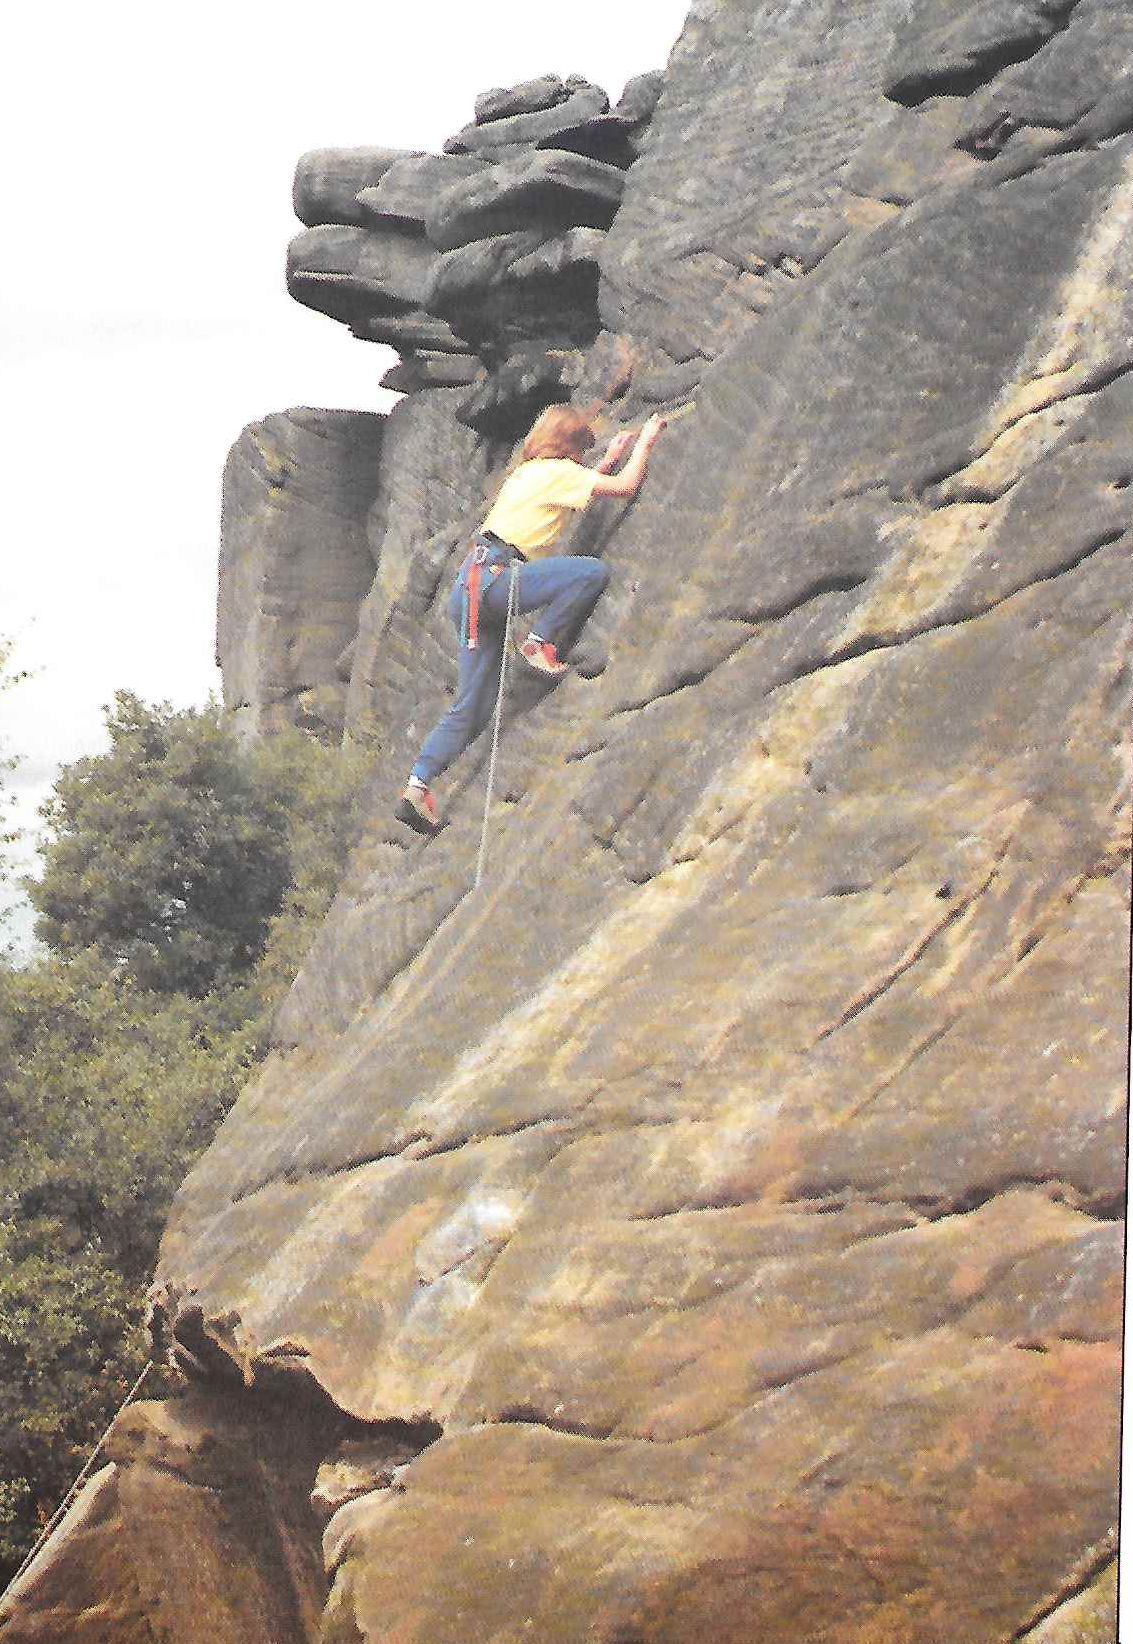
\includegraphics[width=.9\linewidth]{./images/Claire_Coates_on_CMC_Slab.jpg}
\caption{\label{fig:org19856a1}
Claire Coates on CMC Slab.}
\end{figure}

\chapter{The Lundy Experience}
\label{sec:org8366245}
\chapterauthor{Steve France}

Sailing across the bobbing sea towards Lundy, we thought we
were so clever!

For the price of a day return we had just enough time to
crack off the "Classic Rock" route called    Devils Slide   . The
ship's time table indicated a visit of three hours on the island
before returning, which was just enough time to walk over to the
other side of the island, climb the route and then walk back. It
was as simple as that. That was until the loudspeaker
announced\ldots{}

"INFORMATION TO THE PASSENGERS - THE SHIP WILL REACH LUNDY
AT FOURTEEN HUNDRED HOURS AND DISEMBARKATION WILL TAKE
APROXIMATELY FORTY FIVE MINUTES. WILL PASSENGERS BE AT THE
EMBARKATION POINT NO LATER THAN SIXTEEN HUNDRED HOURS. THANK
YOU."

"Hang on, I thought we had three hours!"

We did, from the ship's arrival to its departure, but
unfortunately  that did not take into account leaving and
boarding.

"Oh No!!"

Ian Lauriston was beginning to look upset at the thought of
wasting all that money on the crossing. We could tell that by the
way his bottom lip started to curl.

"Wait a minute, we can still do it if we run, but we will
have to make sure that we are first off the ship."

We all reluctantly agreed to give it a go, all except my
wife Serina, who was totally repulsed by the idea of running!

That left four of us  myself and Ian plus Debbie Hall and
Rodger C.  nicknamed, Codger , all waiting in the queue trying to
get off that damn ship.

Dry land came thirty minutes later leaving one and a quarter
hours left to find the route, climb it and get back. We ran.

Navigation was easy due to the fact there was only one path
\begin{itemize}
\item from one side of the island to the other - and by the time we
\end{itemize}
located the top of the rock route, it was time to head back.

Thirty minutes left!  ,
Ian and Codger lost their bottle and with hearts pounding,
started to run back to the ship.  I was determined not to waste
my investment so, without hesitation, started scrambling down the
descent gully to the base of the slab.  Debbie shouted "Could I
have a go?" Time was pressing. A roped ascent?  Not on your
nellie!

Running up the slab I met Debbie below the top pitch,
dumbstruck from witnessing  300 feet of climbing in one and a
half minutes.  The feat was due not so much to climbing skill but
more to the superb friction of the granite.  She threw me the
rope.

"I'm determined to climb the last pitch at least!" she
screamed.

Debbie was very keen - what could I do but take the rope for
her to follow?

The last pitch of    Devils Slide    is the crux and the best
pitch of the route and she enjoyed it, but not the sound of the
ship's horn far away in the distance.

Fifteen minutes left!

"For God's sake Debbie,  go. I'll catch up with you as soon
as I've coiled this rope."

"Please, I used the rope, let me coil it."

"Don't be gallant, go!"

Reluctantly she scrambled over the cliff top in her usual
care free manner and quickly disappeared from sight. Three
minutes later I emerged onto the skyline.

What followed was the run of my life: SACC race in under
thirty minutes!  It must have been, because I caught up Ian and
Codger panting down the path.  Another blast from the ship's horn
turned Ian's face ashen.

"Where's Debbie?"

"She must be here, because there is only one path and I
certainly haven't passed her."

We stood there, frozen to the spot. At this point there was
another blast from the ship.

After a brief discussion we realised that she must have gone
to the opposite side of the island. Should we wait or\ldots{} Another
blast from the ship sent us running towards the beach to be
greeted by Serina, close to tears, with the last boat waiting to
sail across the short distance to the ship. -
"But you can't go and leave our friend behind on the
island," pleaded Ian to the seaman.

"We must leave NOW!" boomed the man, sympathetic but stern.

It was at this point that Ian gallantly volunteered to stay
behind and search the bleak moors for poor Debbie, but again he
was rebuffed.

"No one is allowed on the island without permission. Please
get on the boat!"

With that, we left our Deb to a fate worse than death, all
alone to doss behind a stone wall or a tuft of grass. We sat
there on the deck, still geared up, rucksacks and ropes all over
the place and surrounded by tourists with slightly bemused
expressions. Then came the announcement on the loudspeaker\ldots{}.

"WILL THE CLIMBING PARTY WHO HAS LEFT A GIRL CLIMBER BEHIND
ON THE ISLAND   to rot  PLEASE COME TO THE BRIDGE AT ONCE!"
All eyes turned our way. I could have died!  The ultimate
indignation.

That evening we never went to the pub. Feeling totally
ashamed of ourselves, we went to bed wondering if she knew which
twinkle in the sky was the Pole Star. Since she had found
difficulty in knowing left from right, there was little chance!
Poor Deb.

The morning came and following the captain's instructions we
phoned a number on the island to see if Deb had been found.  She
had, and there she was, on the line!

"Hullo Debbie, are you alright?" piped Ian.

"Yes thanks," replied Deb. "I found this lighthouse and they
were having a party inside - they invited me in and gave me free
drinks and food, accommodation for the night and a huge
breakfast. I've had a whale of a time!"

We waited at the dockside that afternoon. Ian brandished a
club, Codger a crowbar  as for me, if I could have reached her I
would have strangled her!
  "Come here Debbie!"
 '

\begin{figure}[htb]
\centering
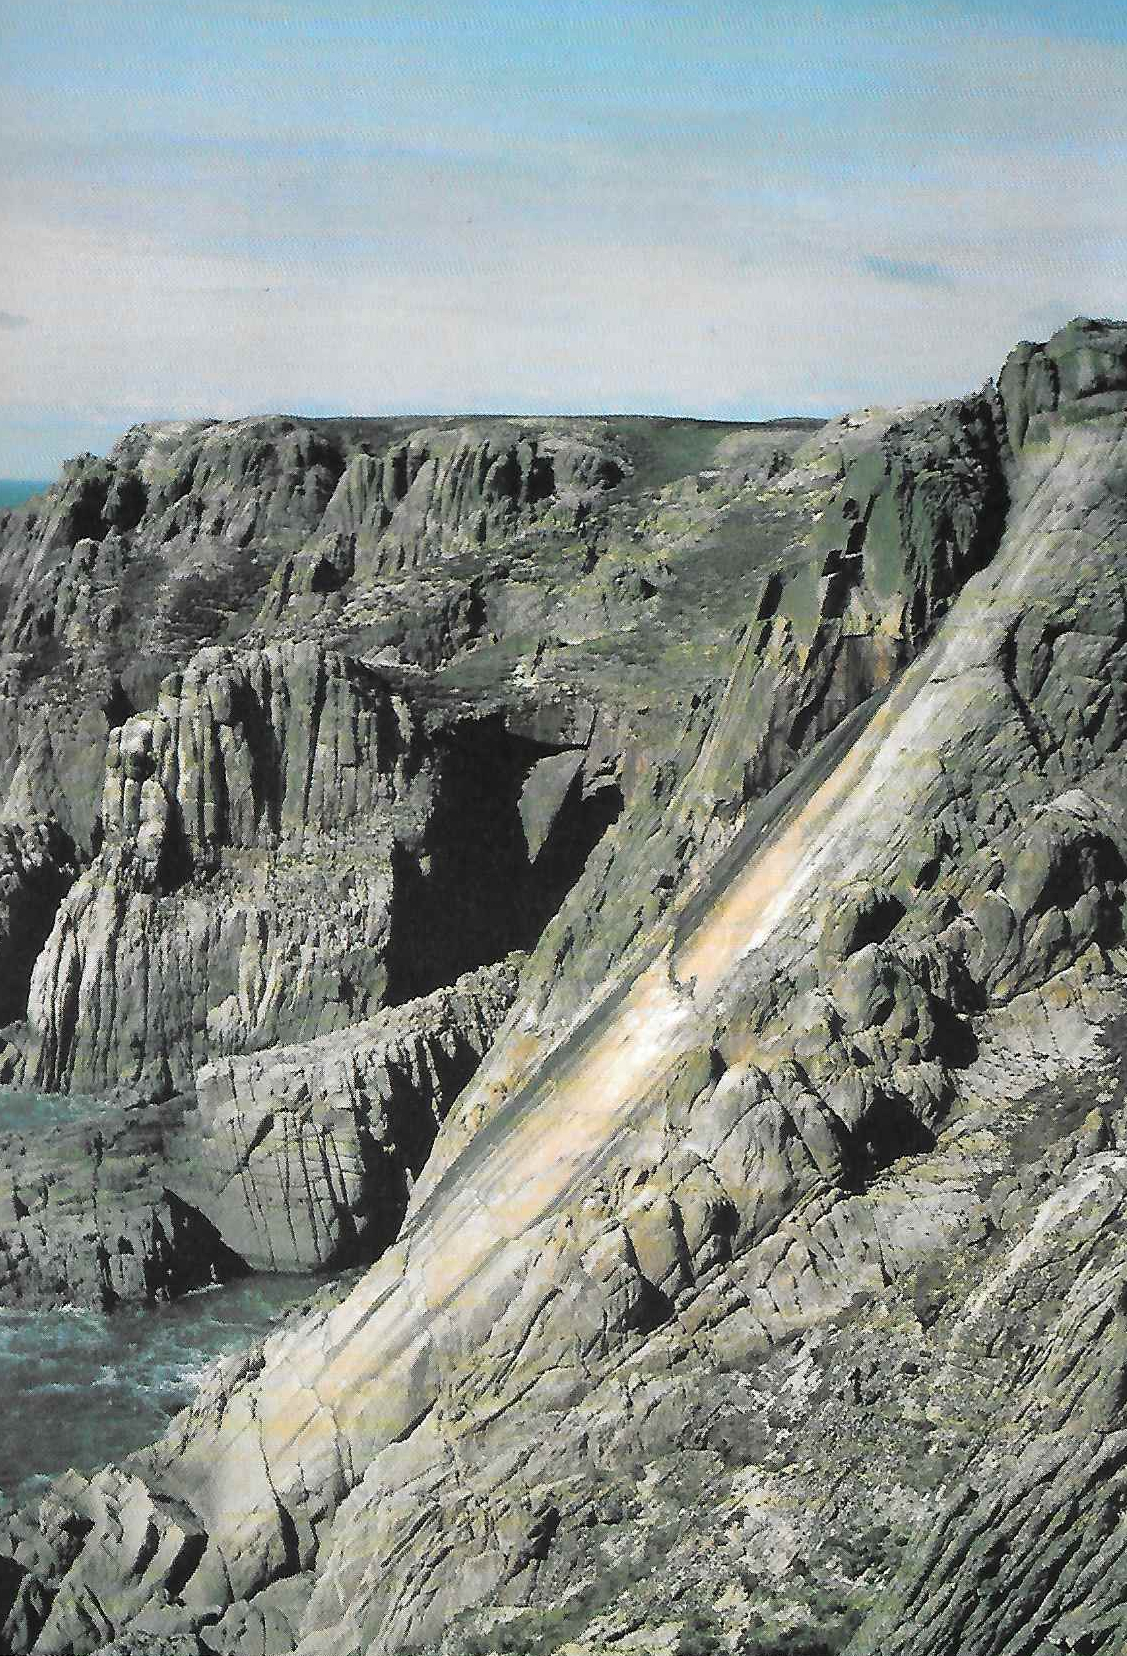
\includegraphics[width=.9\linewidth]{./images/Devils_Slide_Lundy.jpg}
\caption{\label{fig:orgc618b34}
Devil's Slide Lundy}
\end{figure}

Missing photo: First Pitch Devils Slide.

\chapter{Pillow on Pillar}
\label{sec:org90133bb}
\chapterauthor{Mary Peace}


Big Al had forgotten to bring the tent and we would have to
collect it on the way although this meant travelling fifteen
miles in the wrong direction. As we managed to miss the correct
turn off the motorway we did in fact travel thirty unnecessary
miles on the southbound carriageway  before we finally headed
north, my ruffled equilibrium soothed by a generous helping of
Alan's smooth, mellow whisky. We arrived eventually at Wasdale,
quickly donning duvets against the cool October air, and helped
Pat to pitch the tent by torchlight. I snuggled down thankfully
into my sleeping bag.

6.00 am - Feet thundered past the tent and I popped my head
out to see Big Al's figure disappearing across the field. Some
members of our party were already on the move. The remaining six
of us emerged rather more slowly and it was a considerable time
later that we started up Black Sail Pass.

Arriving at the col, we took the climbers' traverse across
the shattered northern slopes of the mountain - our destination
Pillar Rock. By 2.00 pm we were at the foot of    New West   , our
chosen route, ready to climb. The rock reared up magnificently
for 300 feet above a fearsome gully. I was impressed! It was very
intimidating. Frankly, I was petrified. It was our very first
long climb.

Our friends  the early risers   were already half way up
their climb by this time. We watched them as we ate our
sandwiches. By the time we were half way up our route, they were
back at the foot of    New West   . They watched us until Pat, who was
leading our rope of three, emerged at the top of the last and
most difficult-looking pitch on the climb  then Big Al shouted
up:

"You got a bit off route there, Pat. You've just finished
the crux pitch of    Sodom   ! And you haven't finished when you reach
the top. It's quite a climb to get back down again."

"You'll be alright" he added. "You've got a rope!" and they
set off back over the Pass to the comforts of the campsite and
the Wasdale Head Hotel.

Sodom was VS. We were supposed to be climbing a V Diff! I
was very much aware both of the fearsome gully 250 feet below and
the impossible-looking pitch above. The fear which tingled
through my veins was for me an entirely new experience.

There was hardly room to move on the tiny stance I was now
sharing with Dick. Older and even less experienced than Pat and
I, Dick was all sinew and guts - motivated completely by
willpower.

"Try standing on my shoulder, Mary" he said.

With this difficult manoeuvre accomplished, I managed to
launch myself into that strenuous VS chimney. My battles with the
capping chock-stone are better not dwelt upon but eventually, and
very thankfully, I found myself up there, actually on top of
Pillar Rock.

What a magnificent place to be! About a quarter of an acre
of rough rock to scramble over, surrounded on all sides by
precipices. Lakeland peaks lay all around us and Ennerdale,
filled with forestry-planted pine trees, stretched from the foot
of our mountain as far as the eye could see. But by now the pale
October sun was looking very low in the sky.

5.00 pm in October.

"How the hell do we get off this Rock?"

Dick and I walked round and round the perimeter looking for
possibilities, whilst Pat manned the top of    New West     or was it
   Sodom   ?  ready to make contact with and offer help to those still
below.It began to feel like evening.

Six members of another party arrived on top, having climbed
up various routes. No-one knew the way down! Eventually,  the
leader of the other party discovered a route he could reverse. He
threw down a rope and proceeded to see his party off. Just as he
said "Good Luck" to me and disappeared over the edge, our last
climber arrived at top of    New West   . Dusk. Lots of rope to
control!

"Sorry - we must keep moving. We've got to get off this damn
Rock."

When we reached the bottom it was dark  by the time we
reached our sacks it was pitch black. Pat's torch  he was the
only person who had one!  enabled us to cross that frightful
gully and traverse just a little way before reaching a tiny
grassy shelf, where we decided it would be prudent to stop.  -
10.30 pm   All clothing donned but no clothing census taken
\begin{itemize}
\item a mistake that. Four of the party were lying close together on
\end{itemize}
a single exposure blanket. Pat and I occupied our only exposure
bag.

Lights. Down there in the Ennerdale valley. Flashing lights
and shouting - but who? We flashed back. Soon they went away
again. They won't come up to get us until morning, I thought,
perhaps the others were managing to get some sleep. Everyone kept
quiet   another mistake, that.

I remember Pillar Rock looming in the darkness, quite near
to us. It was like being surrounded by black velvet, not a
flicker of light anywhere, just a vague paler shade of black in
the sky over Scarth Gap. I remember the plastic of the exposure
bag flapping round my face in the strong gusts of wind  I
remember being aware that we had slipped a little way down
towards the edge of our grassy shelf where the mountain dropped
away into the darkness  and I remember everyone suddenly becoming
alert and aware as the lights of vehicles appeared down below,
streaming up the Ennerdale valley and coming to a halt at the end
of the road. We could hear a dog barking. Six little lights
formed a crocodile and started up the mountain. Cockermouth
Rescue Team had arrived.

Our party now stirred itself. Two different members of the
party took their turn in the exposure bag and we wrapped up a
third in the blanket. It was at that point we discovered he was
only wearing jeans! We nibbled Turkish Delight as we watched
those torchlights moving up the mountain. I will never forget
that sight, or the magnificent men who reached us some forty
minutes later  the hot sweet milkless tea they gave us  what
nectar! , the clothing, the bars of chocolate, the big alsatian
dog and their radio call sign:  "Poppopoppoff".

"Okay, we've found all six of them. No-one hurt. Over."

We each had a personal escort down, in spite of which Pat
had a rather nasty fall. Near the bottom of the mountain the
Warden from Black Sail Youth Hostel was waiting and as we walked
the last half mile to the Hostel it started to rain. Eventually
we found ourselves sipping hot soup in the Hostel and enjoying
the friendly hospitality which the Warden provided. We were very
glad not to be still out there on the mountain.

We had hardly finished breakfast next morning when our CMC
escort arrived to see us safely back over the mountain pass to a
reunion with our friends at Wasdale. Not abandoned to our fate
after all!

\chapter{The Siege of Clachaig Gully}
\label{sec:orgb9cbb70}
\chapterauthor{Alan Fowler}

On one of the earliest Glencoe meets the sun actually shone
on both the Saturday and the Sunday! Faced with the long drive
home that night, a group of us looked for a climb which didn't
involve a long approach and decided on    Clachaig Gully   . We packed
up and were about to start out from Lagangarbh when someone asked
what we had in mind.

"Clachaig Gully? That sounds like a good idea. Mind if I
come along?"

By the time we had set off from the pub car park the numbers
had swollen to about twelve and it had the makings of a good
epic. I can't remember all the names but Mike Anderson, Ashley
Turner and Dick Arnold were definitely among the team.

The early pitches went well and we made rapid progress
despite the numbers. Then we came to the cave pitch  Mike led
this and I followed. No one else felt like leading it so, sitting
on the little saddle at the top of the pitch, I began top roping
people and lowering them down the other side of the ledge where
they could unrope and walk into the bed of the gully. It was
pleasant enough sitting up there in the sunshine and when the
last man was up I swung down to the ledge, coiled the rope and
walked up the gully fully expecting to find a top rope on the
next pitch. What greeted me was a very glum circle of people.

"Your pitch" said Mike, before I could object. This was the
famous Jericho Wall, dripping in water and slightly overhanging.
My first attempts all ended in failure, which was in itself only
slightly frustrating compared to the added annoyance caused by
the water streaming down my shirt sleeves. The problem was
getting a foot onto a small incut hold about eight feet up  the
slime covered wall offered no positive foothold and what hand
holds there may have been were similarly slippery.

Reversing the route was totally out of the question so, rummaging in
my sack, I dragged out my secret weapon. A peg!  This, placed at head
height, gave me enough assistance to gain the foothold the holds above
were then within reach and the rest of the wall was easier. I threw
the rope into the gully and the rest of the team began their
ascent. About half the team were up when I heard the clatter of
equipment as another group reached the top of the cave pitch. Then the
distinctive twang of a Glasgow accent drifted up.  If they found us
using a peg on their route there would be a lynching!

"Get that peg out quick, the Scots are coming," I shouted
down. Two taps of the hammer and the evidence of our
transgression was removed.

The Scots were left to climb the pitch by their own devices,
giving us enough time to implement our escape in the best Castle
traditions of tact, diplomacy\ldots{} and self preservation.
[[\begin{figure}[htb]
\centering
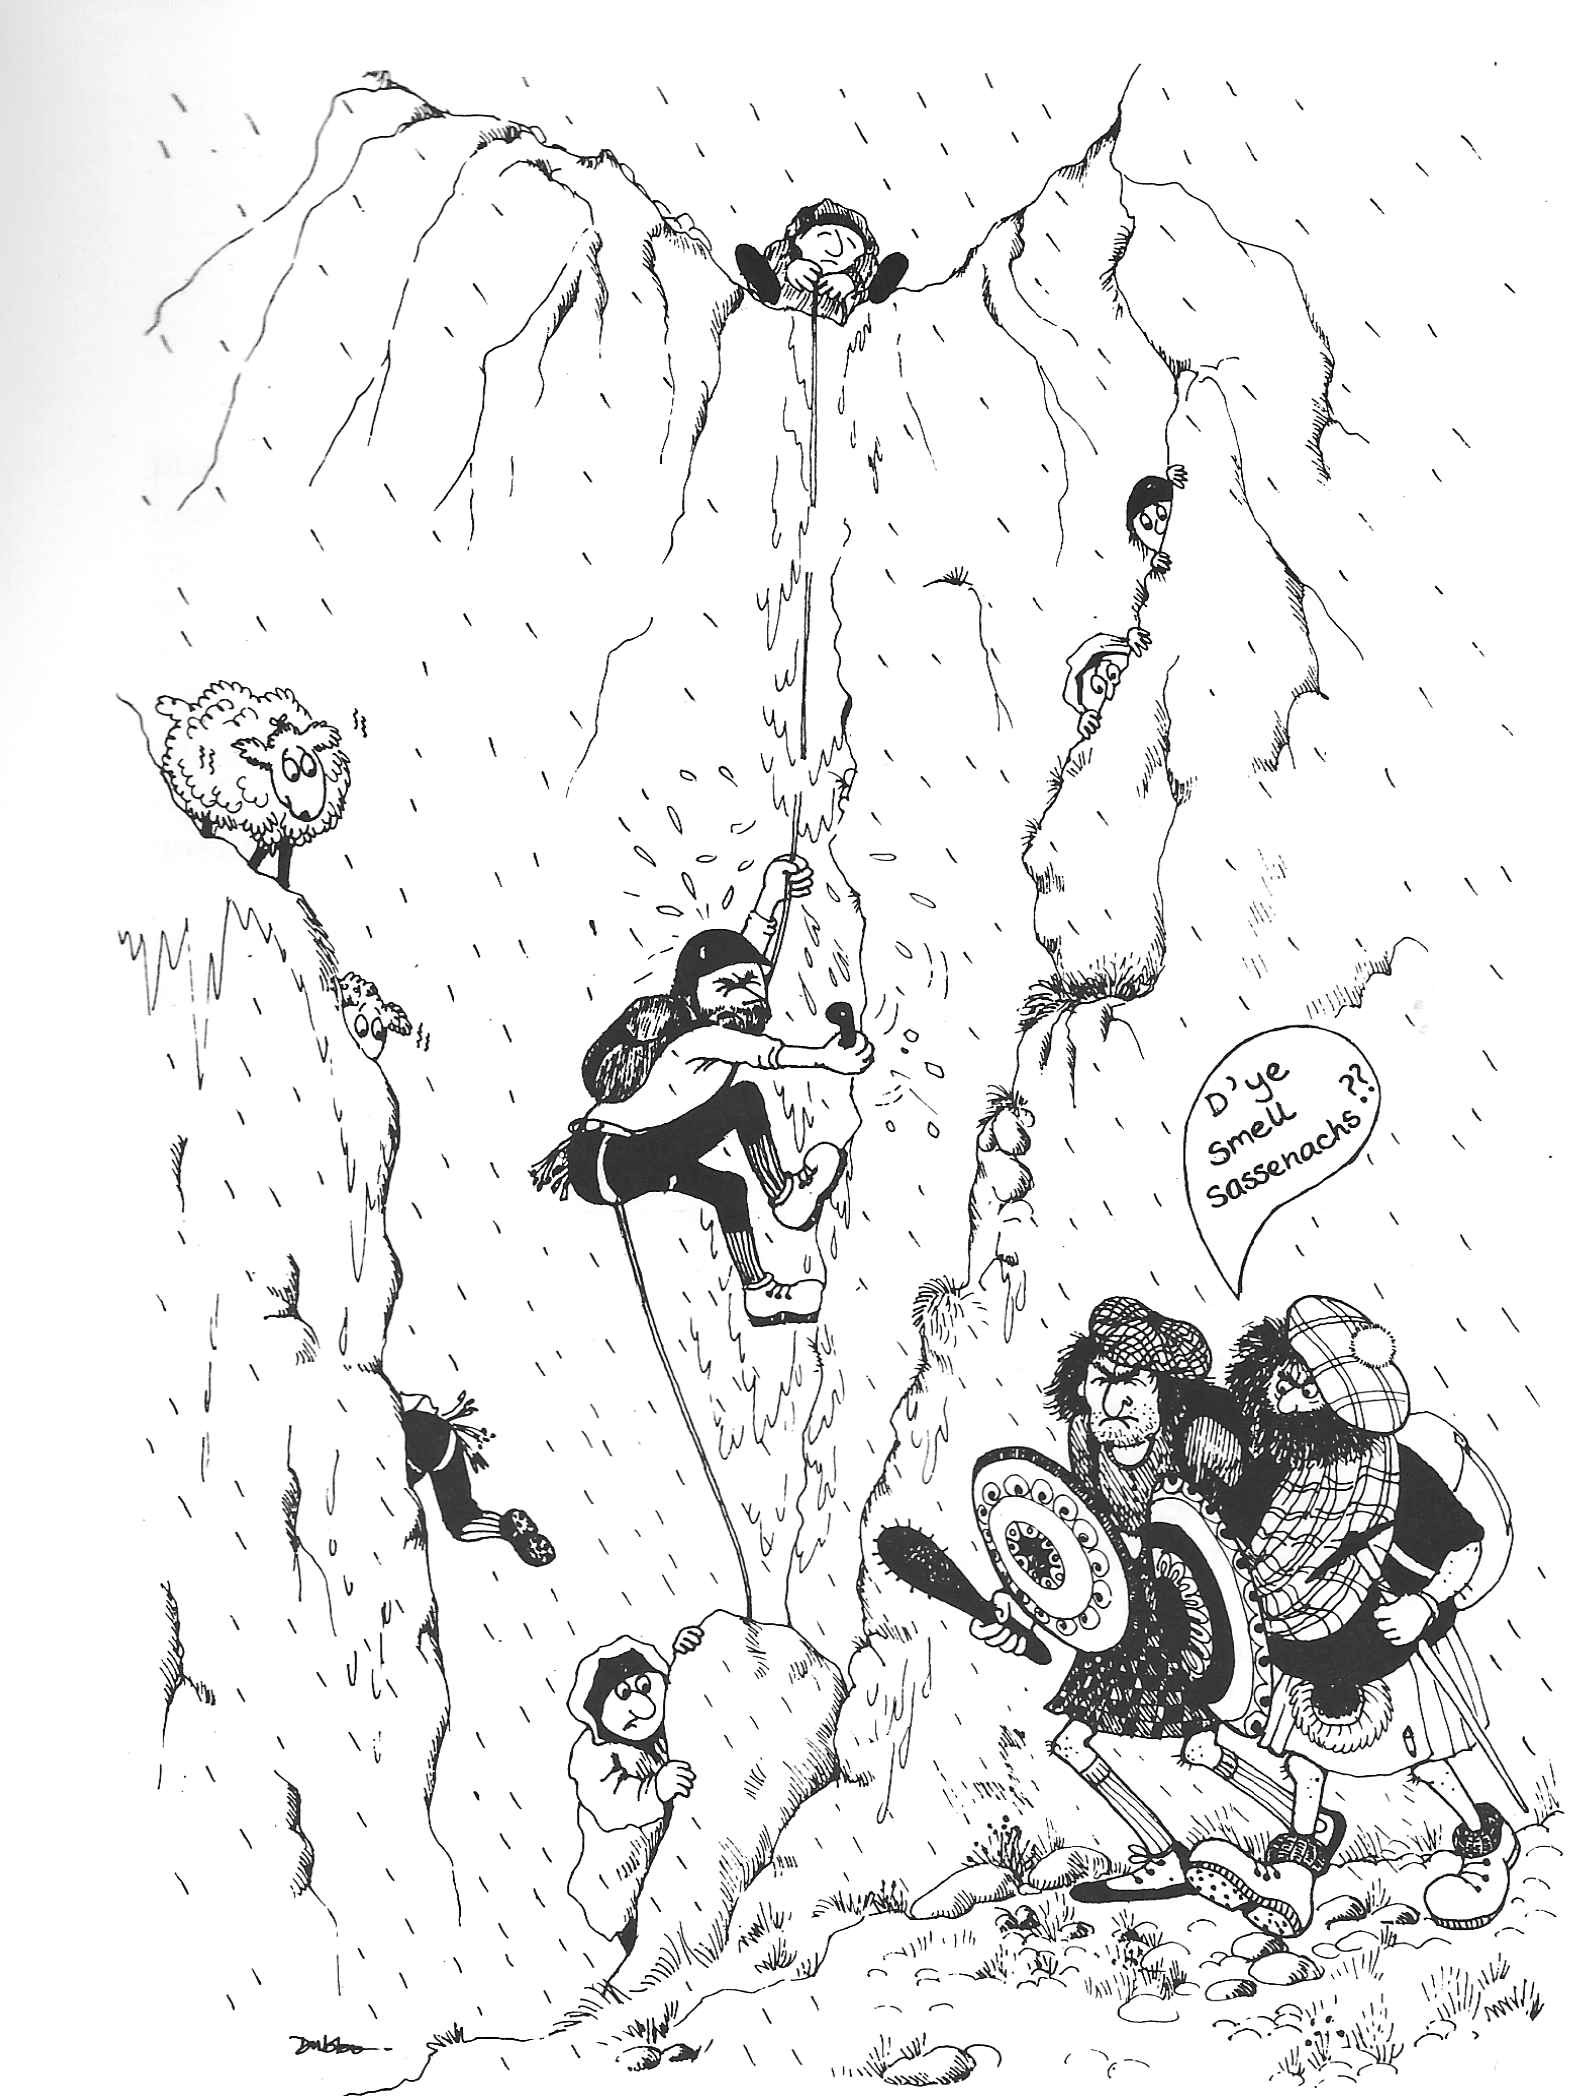
\includegraphics[width=.9\linewidth]{./images/Cartoon_02.jpg}
\caption{\label{fig:org9eea6cc}
The Siege of Clachaig Gully}
\end{figure}]

\chapter{The Castle Wall}
\label{sec:orge68a776}
\chapterauthor{Steve France}

Indoor climbing walls have long provided both amusement and bemusement
to climbers and spectators alike. The Castle climbing creation is no
different in that respect but, due to its unique location in the
clubroom, its frequency of use tends to reflect certain phases of
interest within the Club. An increase in the wall's popularity usually
occurs at times when there is an influx of new members or novices, or
when there is a strong climbing contingency.

The climbing wall's construction and development in the early
seventies paved the way for the sudden burst of interest it received
between 1978 and 1981.  This was chiefly due to the production of the
first ever guide book to the outcrop and a large enthusiastic group of
climbing members. Competition within the Club reached a peak in 1980
and this is reflected by the new routes section in the back of the
guide book, a good example being the route called The Merry Monk .
This hotly denounced route was climbed by Tom Benson with the use of a
hold that was allegedly out of bounds half an inch to the right! . It
was quickly climbed without the use of the offending hold by Steve
France who renamed it Short Black Curly Hair but the arguments did not
end there due to mounting ethical disagreements. Both Tom himself and
Richard Staniforth who also attempted to "take the glory" were over
six feet tall and could easily reach past the crux move - much to the
annoyance of Steve who could not do it without making a ridiculously
hard move. Despite several weeks of contemptuous lip the true claimant
to the fourteen inches of newly climbed rock was never decided - but
who cares anyway?

Steve Hartland, as a reflection of the times, promptly free climbed
all the aid routes, and for entertainment Keith Naylor thrust his
person onto the rock to create Lunge or Plunge . The route should
really have been named Lunge and Plunge, since it allowed a means
of reaching the top using only two footholds and one hand hold. If
you think that sounds amazing then ponder over the fact that The
Crack was climbed from top to bottom using only one hand jam. You
are advised not to attempt this unless you are proficient at
mid-air jamming!

The Club supplies various items of equipment for members or visitors
wishing to climb on the wall, including ropes, helmets, and various
old pairs of rock boots. It is always stressed that climbing is at
one's own risk and that utmost care is required.

The Castle must be one of the few clubs to have its own climbing
wall - so why not give it a go?

Please Note\ldots{}. all routes graded over HVS can only be climbed wearing
lurid coloured tights and headband. Please also remember that the use
of chalk is forbidden!

Good Luck.
\begin{figure}[htb]
\centering
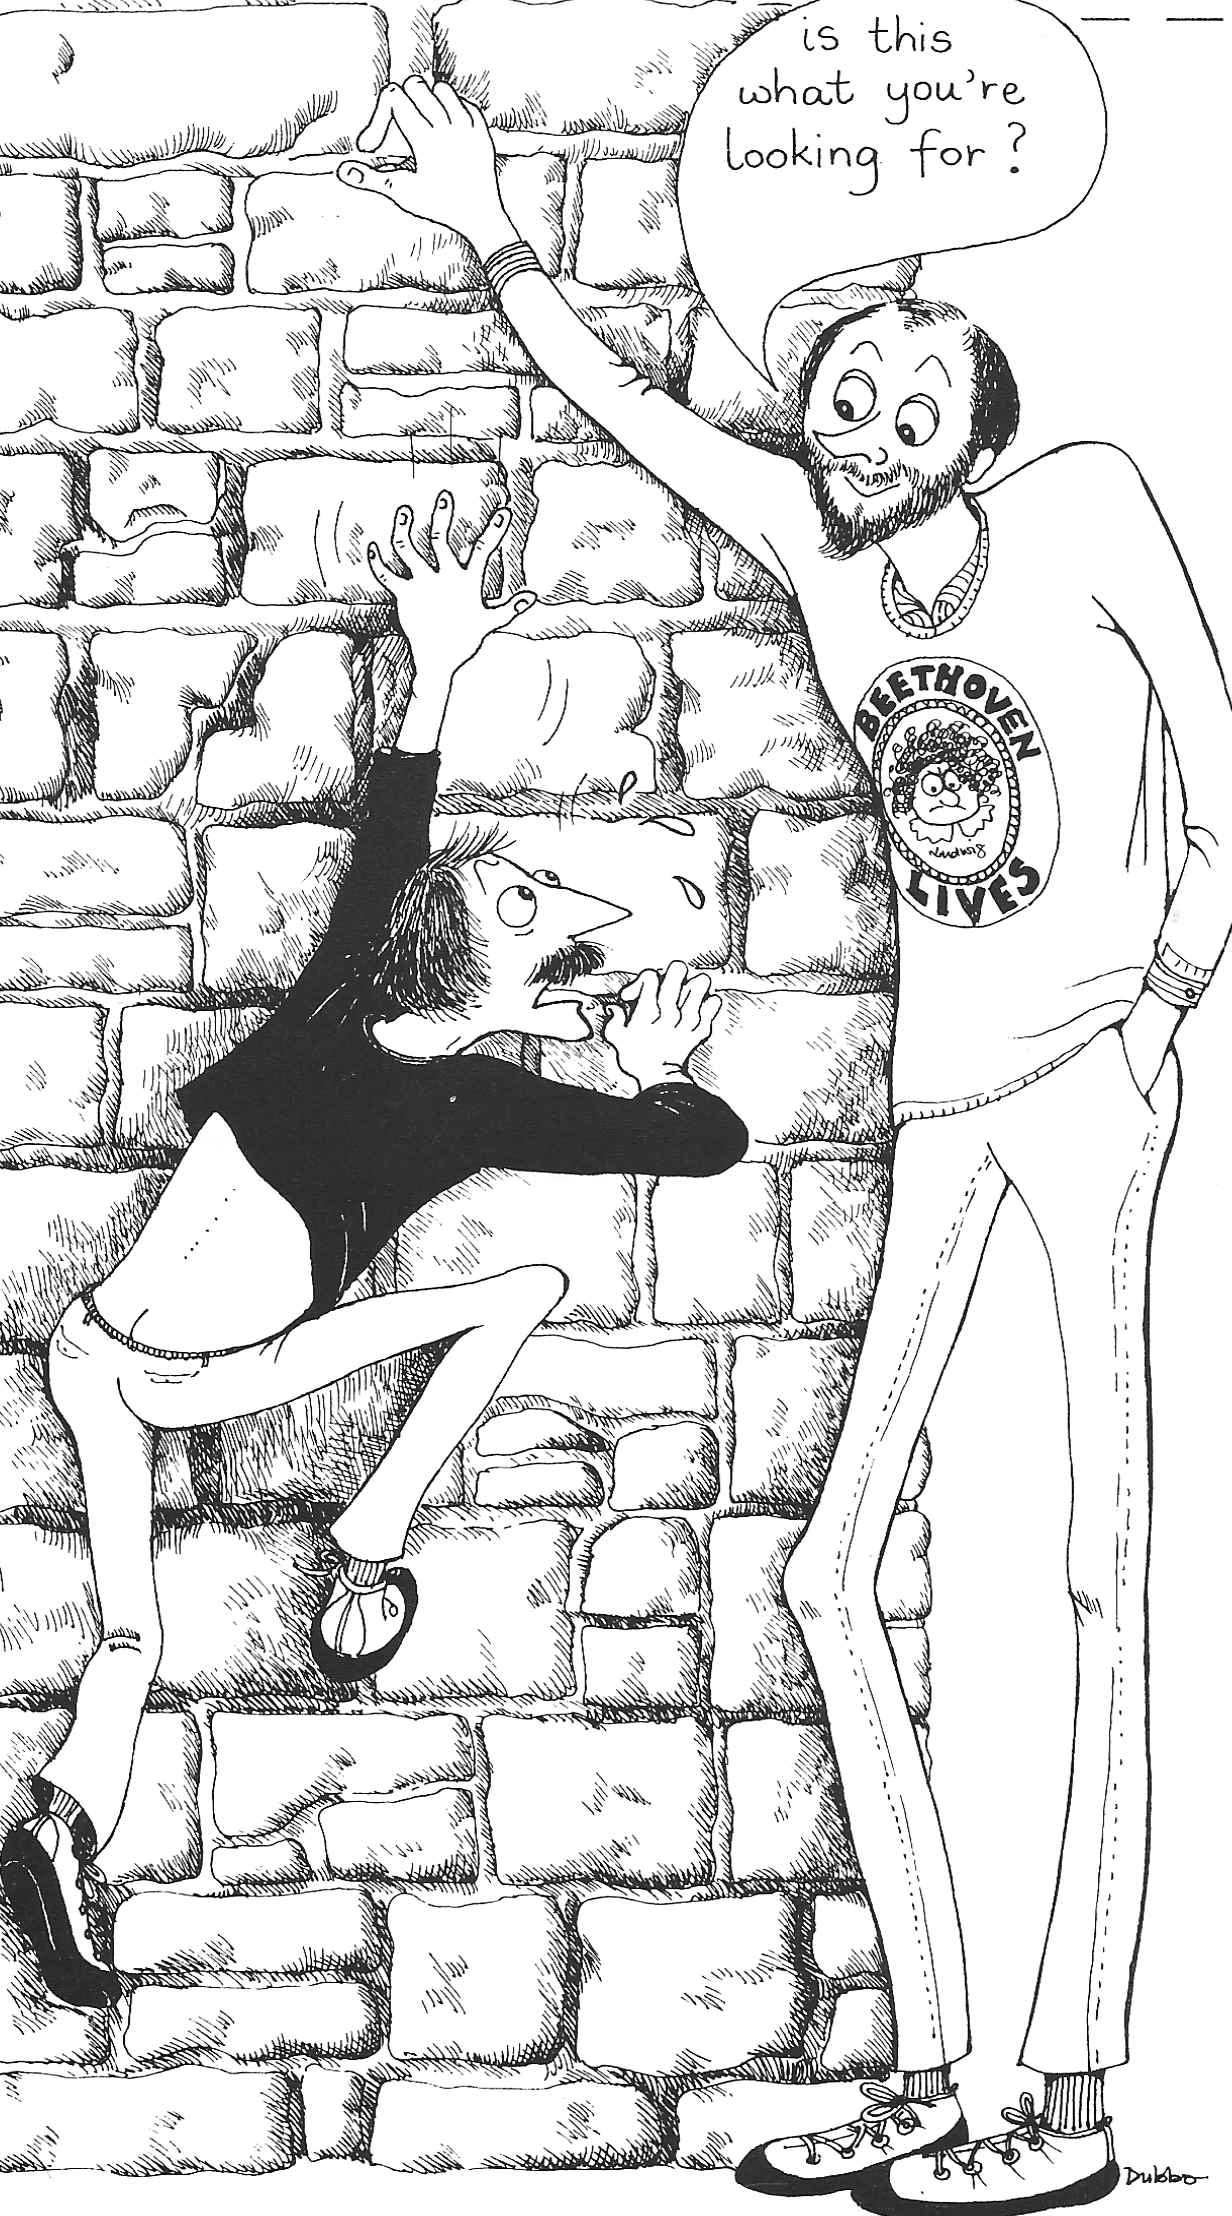
\includegraphics[width=.9\linewidth]{./images/Cartoon_03.jpg}
\caption{\label{fig:org986344e}
The Castle Wall}
\end{figure}

\chapter{A Cautionary Winter's Tale}
\label{sec:orgba921e9}
\chapterauthor{Dave Kime}


It was the Club's Easter Meet in Glenshee 1978. Base camp
was established at our now traditional wild campsite by the
Clunie Water on the Braemar side of the Cairnwell. Good Friday
saw Harry, Charles, Anne, Jenny and myself crammed into the Maxi
with packs and camping gear for four days. The car was left in
the ski car park and a note  containing, in accordance with
official recommendations, details of party and destination  was
left at the ticket office - the official Mountain Rescue Centre.
We struggled, with full packs, up the chair lift and off to Loch
Vrotachan. Anne appeared somewhat nervous and apprehensive - she
said it was because she hadn't done much skiing, but in
retrospect I suspect it was well justified apprehension at the
thought of spending three nights with Harry and Charles.

The weather worsened as we skinned  up to Carn a'Gheoidh,
and by Loch nan Eun spindrift was hurtling across the frozen
waters. Hardly a suitable campsite, but by dropping to the north
we found enough shelter by a peat hag to sort gear and pitch
camp. The peat was rock hard, so the tent was anchored only to
pegs buried in snow and well trampled.  Water was found at the
bottom of an  eight feet deep pot hole in the snow  with rather
delicate access. The two parties disappeared into their tents for
the night and emerged only when driven by overwhelming natural
necessity. Gales and snow swept around all night, occasionally
punctuated by  mysterious noises from the other tent. Even a cry
of help would not get us out tonight! Meanwhile, unbeknown to us,
back in civilization, police forces in five counties were
mobilising.

Come morning, the tent had survived and so had Anne. A sunny
start had us doing the Beinn Iutharns but we were soon back in
clag and Charles was having problems with his new high-tech
sticky skins which had taken a dislike to the cold weather. Gales
rose again that night and rising above them were intermittent
muffled screams. We pulled the hoods of our ducks over our heads
and pretended not to hear.

The tent had shrunk by next morning to half its former size
as the weight of snow pressed in. Charles and Harry assured us
that Anne was alright   she was less sure. Four of us skinned up
to Carn an Righ followed by Charles towing his skinless skis -
he'd make a good doggie-walker! A superb run in powder snow down
to Gleann Mor made it all worthwhile. Back at camp, the bags were
getting damp and by next morning only the tips of the tent poles
were visible. With some difficulty, the pegs were unburied and
with full packs we had a great ski down to the Baddoch Burn  then
after a last skin up to Loch Vrotachan, we joined the crowds on
the Cairnwell run.

The car was still there, but Anne was convinced that someone
had been through her handbag but not taken any money - three
nights with Harry and Charles does take a little getting over!
Mugs of coffee in the cafe where we heard that Sheffield had been
cut off from the world, airports closed and the Glenshee Mountain
Rescue called out. Well, it had been a bit wild. A little later I
wandered over to the counter to report our safe return.

"Er, yes, er, just a, er, minute" said the lad  and
disappeared to return with the manager and Leader of the Mountain
Rescue Team.

Over the next few weeks the story was pieced together. By
nine at night the white Maxi stood in splendid isolation in the
middle of the empty car park. The police were informed and the
car number dispatched for the Swansea computer to work on.
Meanwhile, back at base Kate and Al had arrived and were settling
in for the night. Kate was rudely disturbed from a privy squat by
powerful torches, Land Rovers and the full might of the Braemar
police force. Somewhat shaken by this disturbance Kate was
interrogated about the whereabouts of the Kime party. The officer
did not react very kindly when told that these malingerers were
camping in the hills. Meanwhile two mountain rescue teams had
assembled and the ski tows were brought into operation to search
for the "lost" skiers.

The Swansea computer had informed the Braemar and Sheffield
constabularies of the identity of the owner of the Maxi.

At Hallamshire Close, Sheffield, the Kime house was empty
so the neighbours were knocked up for questioning.

"Oh, they're camping in Scotland somewhere."

"Yes, we've just found their car - nothing in it but an old
pair of wellington boots and a ladies handbag." ,!
Leaving our friends to the vision of their eccentric
neighbours barefoot on the mountain, the officers departed. An
hour later, our friends phoned West Bar police station in
Sheffield when they remembered where Jenny's father worked.
Across the Pennines, the University night porter was awoken from
his duties and questioned as to the whereabouts of the Professor
of Engineering. Lancaster Constabulary found his house empty as
well.

"He's in Scotland" said the neighbours   "at the cottage."

No way were the Inverness Constabulary in Fort William going
to drive two hours to that address at that time of night: a phone
call to their local contact would have to suffice. Campbell
Morrison was dragged from behind the bar at the Clan to drive
three miles, wake up the Professor and bring him to the phone.

"They're camping in the hills and they know what they're
doing. Call your rescue off!"

The message got back to Braemar and all teams were stood
down. The Braemar police, on returning to base, stopped by to
rouse Kate and Al again in order to tell them in no uncertain
terms that Dr. Kime was to report to the police station
IMMEDIATELY he got back.

Next morning the staff were back  at work at the ski centre
and as the ticket office opened, the lad put his hand in his
pocket.

"Och, Hamish, a laddie left me this note yesterd\ldots{}.." As
Hamish said: "The lads dealt with him - he won't forget again in
a hurry."

Back to base camp in the glen where we discovered that our
tent had disappeared, then found the shreds neatly folded and
packed in Charles' tent. Kate and Al returned from a day of
ticking and passed on the message.  ,   -  Down to Braemar.

"My name's Kime, I believe you want to question me in
connection with\ldots{}"

"Och, that fiasco on Friday, come on in."

Somewhere in all this there must be a moral   about parked
cars, about leaving  notes to the  police, and rescue teams being
called out unnecessarily, and of training and certificates  and
of the freedom to roam the hills unhindered and to  take
responsibility for one's own safety and actions?

\chapter{Rumble Groove}
\label{sec:org95c0f35}
\chapterauthor{by Marian Birkett}

What do I remember about The Castle? Well it's people, days
out climbing, for instance days with Dave, well known for his
enthusiasm for climbing anything, anytime   although preferably a
traditional route on Kinder. If it's a vegetated chimney and it's
just starting to rain, well that's approaching Nirvana. The ideal
route description might be, "Climb straight up for 200 feet with
much botanical interest  a fine ten foot chimney then leads to
the top. First ascent 1892."

One day Rosie, Dave and I headed for a Peak District
equivalent: short, insignificant and green, on some boulders
which think they're a crag. Yes, the  in famous  Rumble Groove  on
Carl Wark. Not heard of the route? You're doing well if you've
heard of the crag!

Dave and Rosie had though, in fact it was Dave's third
attempt at this route. He had spent several hours pitting his
strength and skill, definitely in that order, against the rock
 it's that sort of route , retreating with bruised arms, legs,
ego, everything. Today would be different.

We approached the crag. Crag, did I say? I noticed some
rocks huddled together.
"That's Carl Wark," said Dave. " Rumble Groove  is well over
to the left there."
"Oh, really?"
"It's super. A real classic."

I tried to sound enthusiastic but failed miserably. We
uncoiled 150 feet of rope, 130 feet of which was totally
unnecessary. Peak District climbing is like that: crags that are
too short, ropes that are too long and, as we were to find out,
cracks that are too wide.

Dave tied on and Rosie belayed, so I was free to escape from
the midges and to wander about looking at the groove from
different angles   none of them in the least encouraging. I
hadn't seen Rosie for a while and we chatted whilst Dave grunted.
After half an hour we'd caught up on all the news  after an hour
we were dragging up insignificant crumbs of gossip.

Dave was struggling. First there's a wide crack leading up
left. The jams are painful, insecure, slimy and the crack
overhangs slightly: a gritstone climber's paradise! Standing on a
rock at the foot of the crack starts you off. Then you must lurch
onto the holds on the left  slight indentations in the vertical
rock  and power your way up the green crack.

The first runner is quite low, only useful if you fall off
the first nine inches of climbing and have an attentive second. A
number forty two hex would have been helpful higher up but Dave
had left it at home. I suggested wedging two hexes together or
passing up a large stone to jam in the crack  I thought the
latter might appeal to his traditional inclinations. But he'd had
enough.

He'd lost count of his attempts to get off the ground and
offered me the rope. Now I can't resist a challenge and certainly
this was one. However, I am a coward and my first priority is
always to get a runner above my head   well, even one a bit
higher than the last would help. Somehow, to hurt yourself
falling off a "Classic Rock" route on Cloggy or Gimmer might be
acceptable, but to fall off a boulder near Carl Wark, well the
indignity  of it all.

So with much ingenuity and a lowering of ethical standards
 this was a traditional route after all  I slammed a Friend in as
high as I could. This superhuman effort reduced me to a quivering
jelly, wobbling back next to Rosie. I quickly returned the rope
to Dave after Rosie had refused it   she's got more sense!
With the confidence of another runner and fresh from a good
rest, Dave attacked the rock with daring spirit. We gave him lots
of encouragement by pointing out that we had only five minutes
left before we were off home and suddenly, to our great surprise
and consternation, he was cheering from the top. Oh no! That
meant that we'd have to do it.

I went next. After an interminable fight in the crack,
leaving it dripping with blood, I emerged secretly vowing never
to let Dave pick the route again. Rosie went next, the fastest
ascent yet.

Our attention was then drawn to the only other route on
these boulders,  Green Crack . A similarly attractive climb, its
name being most descriptive  a green, slimy, rounded crack. They
gave me the rope and, teetering and complaining, I reached the
top. I was surprised when they declared it twice as nasty as
 Rumble Groove . So if you're wanting to reduce someone's
enthusiasm for grit, I thoroughly recommend a day out somewhere
near Carl Wark. As for climbing with Dave\ldots{} you have been
warned!

\chapter{Ridge Routes in the Land of The Rising Sun}
\label{sec:org3f59717}
\chapterauthor{Dave Kime}

This area had long been neglected by the Club, although
older members could recall long days spent hacking through ivy on
exposed ridges and ascents of swaying trees. Spurred on by these
legends and by reports that chunks of stone were falling off some
of the routes, the Club held several meets in this area so close
and so unfamiliar to most Club members   the clubroom roof.
These meets were inaugurated by Sean, who unfortunately was
unable to ensure good weather. The first one was cancelled by an
eighteen inch snowfall and the second gave us a wonderful
experience of what it would be like to install a window in the
middle of Kinder Downfall. We had a chance to look at the roof
only very briefly while Andy indulged in the legendary pastime of
ivy clipping. We were by now a little more aware of the problems
we had to tackle and the committee set aside three further
Saturdays for the purpose.

Our next meet was somewhat exploratory but we found a number
of loose slates and a decaying chimney on the outside. Andy,
Charles and Frank constructed a spider's web between trees,
telegraph poles and the chimney stack and set about
reconstruction, whilst Dave and Tom prepared Ready Mix, filled
the gaping holes under the eaves and did some pointing. A
successful day, marred only by the sight of a forlorn starling
looking for the entrance to its nest next to the chimney stack.
The major problem then remaining was how best to stop the
mortar falling off the inside of the roof and annihilating the
members. We had many ideas but little real knowledge. However,
fate was kind and brought us a new member, Chris, who in a rash
moment admitted he was a builder and in an even rasher moment
volunteered to come on the next meet. Perhaps he had seen our new
chimney stack and realised that we were real craftsmen, or
perhaps he had seen the chimney stack and realised \ldots{}

Two weeks later we met again. The chimney was still standing
and Chris was very polite about our work but we hoped he wouldn't
look too closely. We were then shown how to use mortar trowels
and since this appeared so easy we got on with the job of
knocking down the eighteenth century mortar whilst Chris fixed
the slates on the roof with a total disregard for the ropes and
ladders with which we had festooned ourselves on the previous
meet. By lunch time the floor was deep in old mortar and we now
had to fill in the holes we had made. This was not as easy as
Chris had made out and a number of us resorted to mortar stuffing
by hand rather than by trowel. While Chris hung to the rafters by
his toe nails and mortared the higher reaches of the roof, Roger
swung from the planks and delivered well aimed dollops down the
neck of anyone who passed below. Andy swung across the walls on
an elaborate arrangement of slings and during his girdle traverse
of the clubroom demolished only two of the spotlights.

Mike and his son Mark joined us for the afternoon and while
Mike filled, Mark delivered pots of gunge to the inaccessible
corners of the clubroom. Disposal of the debris took quite some
time, as did the removal of Roger's wedges of mortar from our
spines. We had at least completed the work at the end of the
clubroom nearest the climbing wall which we now felt was a little
safer, even if the holds did require a dusting. A rather smaller
party met to deal with the remainder of the roof. With the
numbers available, we also managed to clear and re point two
sections above the upstairs room, which offered rather less of a
challenge than the previous week due to their accessibility.
Whenever we plan to work on  the roof, come along: it's great fun
and Your Club Needs You.

So, if you see a member in climbing gear with an ashen face
and a concrete helmet, he's probably just been climbing in the
Land of The Rising Sun.

\chapter{The Search for The Drunken Duck or "Doesn't Anybody Want to Buy Any Petrol?"}
\label{sec:org5a4661b}
\chapterauthor{Alan Fowler}

It was a fairly typical weekend in Langdale. It had rained
on and off  more on than off  all Saturday. Some of us had
convincingly demonstrated that one could get just as wet in half
a day as in a full day, by walking up Side Pike in a monsoon.
After a meal back at the campsite, the talk naturally
centred on which pub we should honour with our presence that
evening.
"How about The Drunken Duck?" I suggested.
"The what? Where's that?"
"It's a pub somewhere between here and Coniston. It's
supposed to have some good sing songs."

Armed with this scant knowledge, a convoy of four vehicles
set forth. A look at the map will show quite a network of minor
roads in this area and with the rain persisting  sic  it down
there was no one around to ask for directions. Suddenly we saw
the lights from a garage ahead so we drove onto the forecourt. A
man ran from the office with a mac over his head, thinking he had
some customers.

"Excuse me. Could you tell me where The Drunken Duck is,
please?"
A look of disappointment crossed his face.
"Yes, next left, then right about half a mile further on."
"Thanks mate."

We drove off into the dark and rain leaving the dampened
attendant to walk back to the shelter of his warm office.
Five minutes later the second car pulled up at the garage.
The attendant again put his mac over his head and ran out.

"Excuse me. Could you tell me where The Drunken Duck is,
please?"
"Yes, next left, then right about half a mile further on."
"Thanks mate."
And that car drove off.

Five minutes later a third car arrived and an even damper
attendant emerged. The same question was asked and the same reply
given. u  A further five minutes and the fourth and final car arrived.
As this car drove off the now soaking attendant was heard to
cry in an agonised voice:
"Doesn't  Anybody  Want to Buy Any Petrol?"
\begin{figure}[htb]
\centering
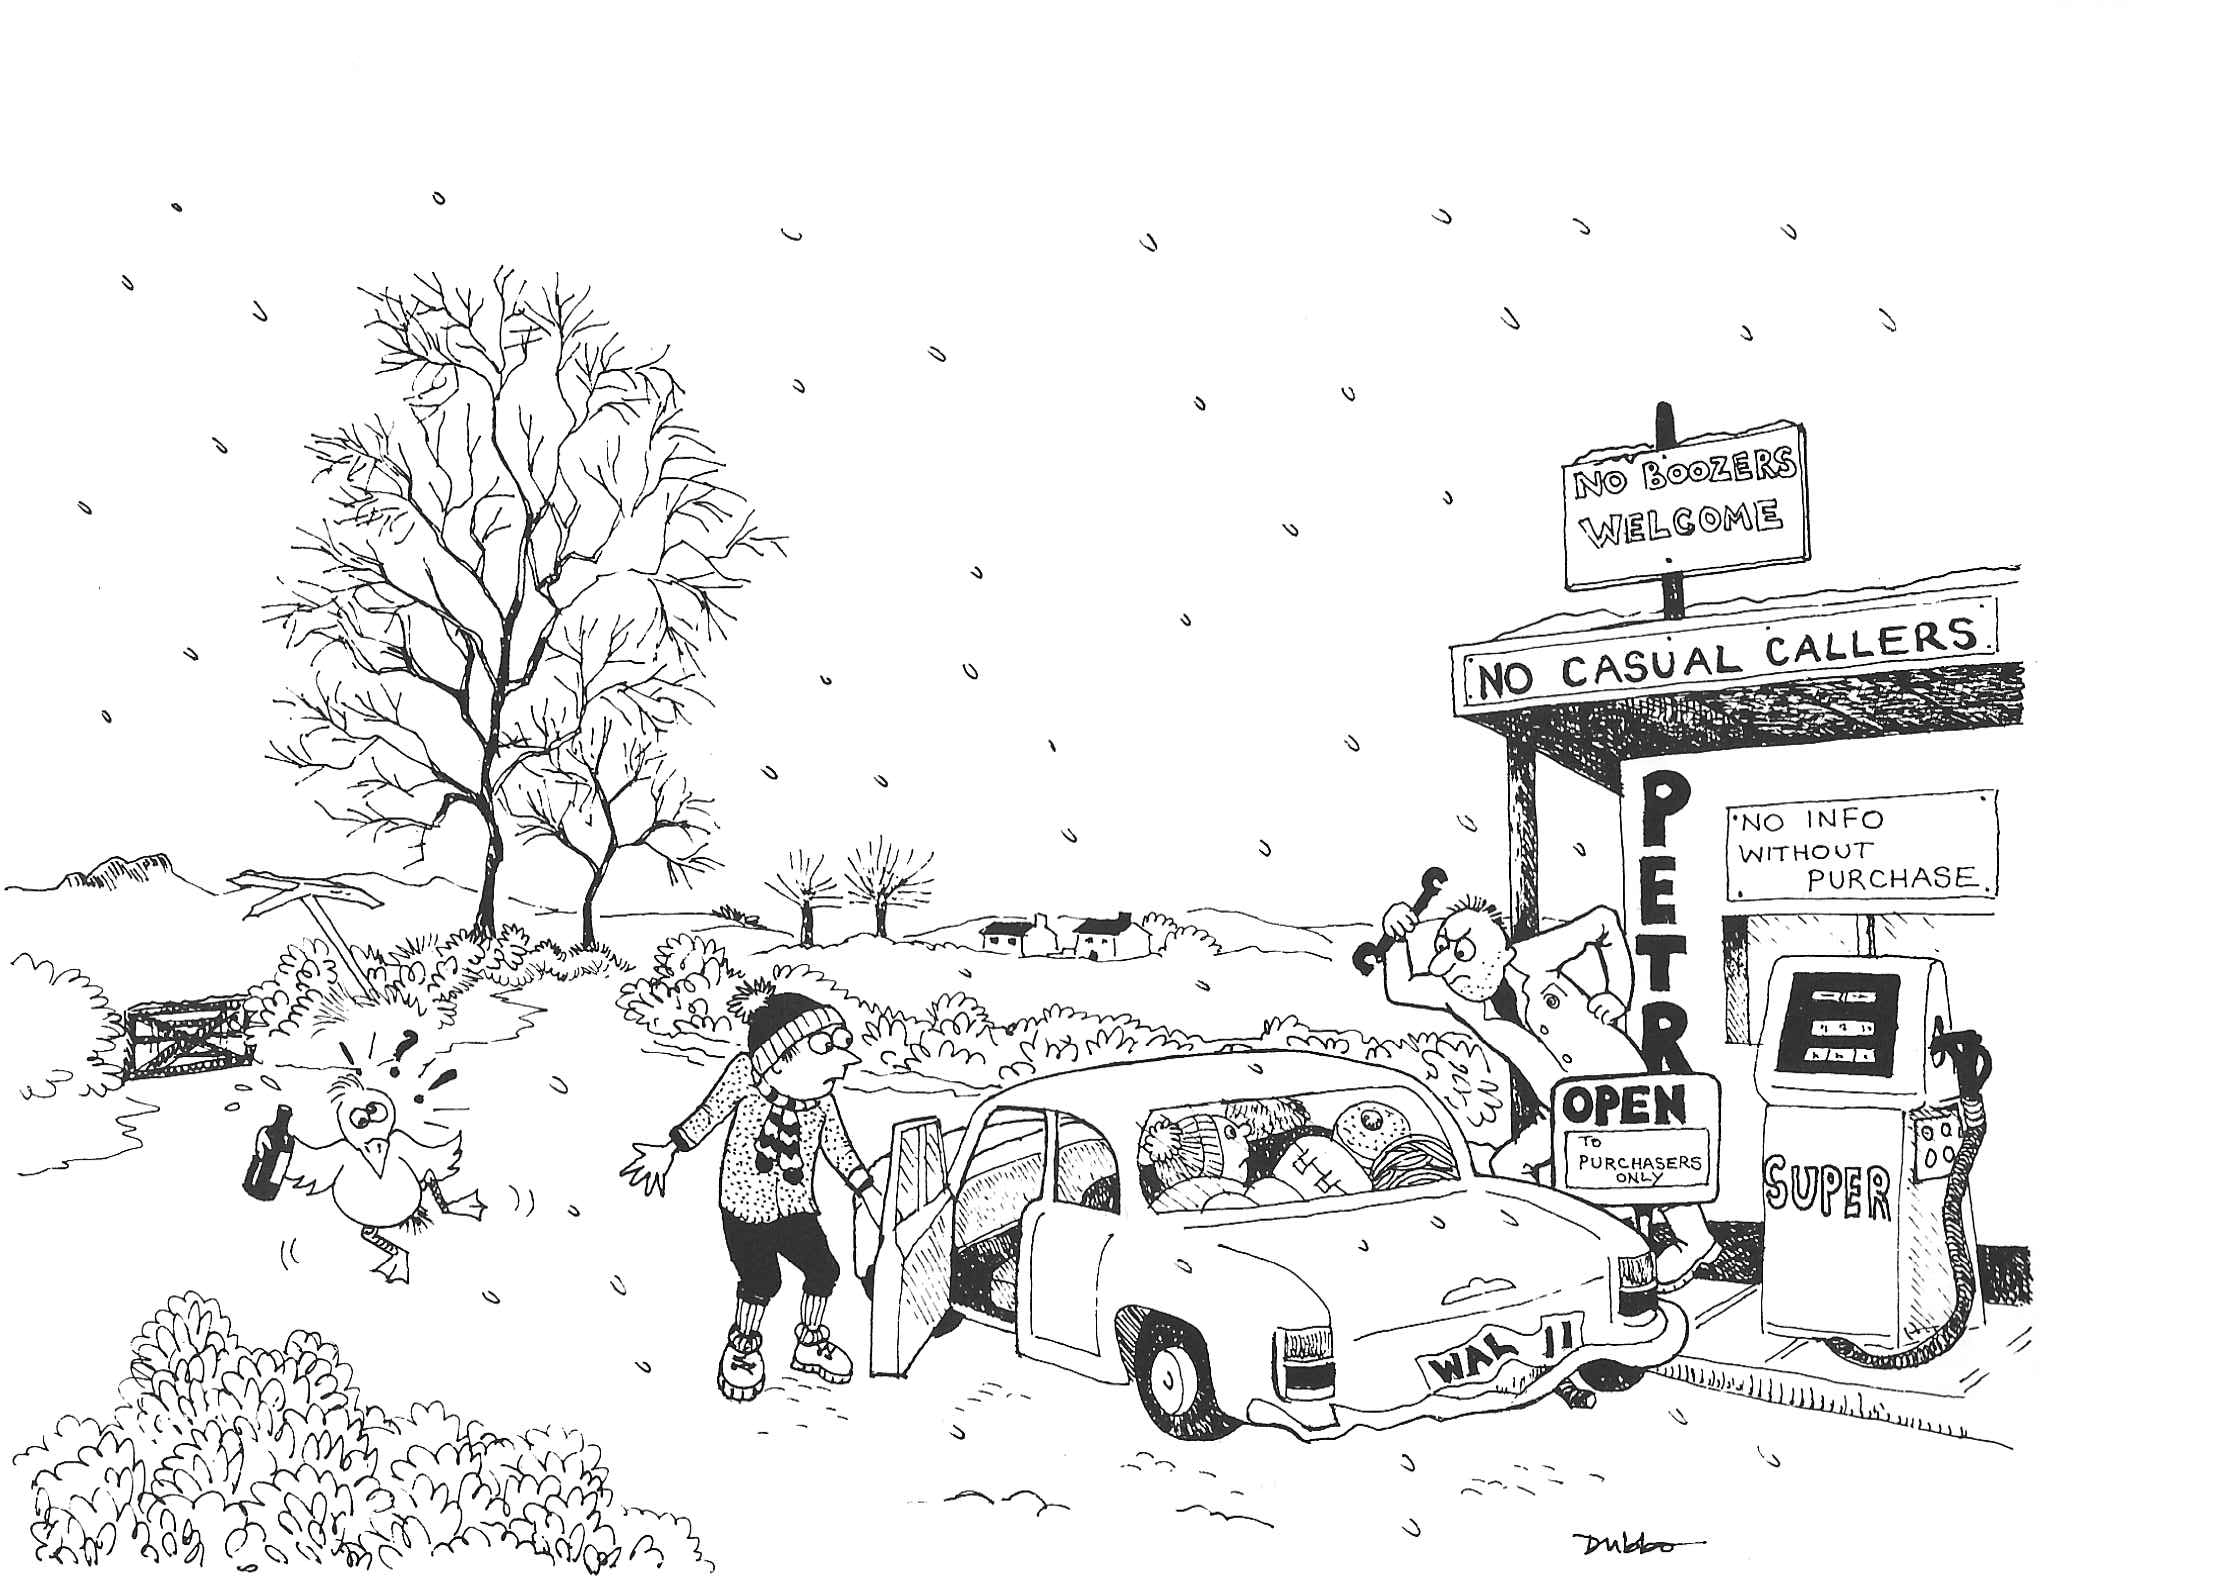
\includegraphics[width=.9\linewidth]{./images/Cartoon_04.jpg}
\caption{\label{fig:org4734f64}
The Search for the Drunken Duck.}
\end{figure}

\chapter{Traverse of the Cuillin Ridge}
\label{sec:org9a3d94f}
\chapterauthor{Andy Smith}

We roused ourselves from our brief but comfortable bivouac
on the  Bealach a' Gharbh Choire, the pale dawn heralding a
perfect Skye day.  Way below us to the east we could see that
remote and magical spot  below the fine peak of Sgurr nan Stri
where the River Coruisk flows  into Loch Scavaig. To the south,
the Small Isles   Soay, Canna, Rhum and  Eigg   were visible
across the calm Hebridean sea, with the fascinating  and shapely
peaks of Rhum in particular attracting the attention.

It was 3.45 am on Tuesday 27th May 1975, the occasion being
the Club's  Spring Bank Holiday meet to the Black Cuillin, the
party  comprising Ronny Hindmoor, John and Lesley Evans, Sean
Jennings,  Andrew Hothersall, Martin Coggins, Anne Pendlebury and
myself. We had  left Glen Brittle at eight the previous evening
and scrambled  up Sron na Ciche via  Collie's Route , reaching the
top in time to see a  gorgeous sunset. Later we had romped along
the crest of the ridge in  bright moonlight, reaching its
southernmost peak, Gars Bheinn, before  heading back to our
bivouac site. Now, with the stars fading rapidly, we  packed our
sacks and climbed to the top of Sgurr Dubh na Da Bheinn  where,
having warmed ourselves up and reached a superb viewpoint, we
paused for breakfast.

Ahead, the jagged crest of the Main Ridge encircled  the
head of Loch Coruisk to its final peak and our ultimate objective
\begin{itemize}
\item Sgurr nan Gillean   a long day's scrambling away but
\end{itemize}
tantalisingly close beyond the coire. We soon reached the famous
Thearlaich Dubh Gap, the first and most  difficult rock pitch of
the day. We abseiled into the Gap and the pitch out of the Gap
was well led, the rest of us thrutching up one way or another -
the rock was  polished and strenuous and we took close on an hour
to get our party of  eight across. We left our sacks whilst
detouring slightly from the Main  Ridge to take in Skye's highest
point, the paramount Sgurr Alasdair  3257 ft .

The next section, around Coire Lagan, is possibly the
finest stretch of the whole trip: Sgurr Thearlaich, an abseil
down to  Bealach Mhic Coinnich, the surprising Collie's Ledge to
Sgurr Mhic  Coinnich and the magnificent scramble over An Stac
culminating in  the unique Inaccessible Pinnacle. We soloed up
the moderate but very  exposed east ridge of the Pinnacle and
abseiled down the short west face. It was now  11 am and getting
very hot  time for lunch.

The ridge becomes sustained, brilliant scrambling:
Banachdich, Thormaid, Ghreadaidh, Mhadaidh, Bidein Druim nan
Ramh, An  Caisteal, Bhairnich, Bruach na Frithe: the roll call of
evocative  Gaelic names familiar to every Skye afficionado. Each
Munro has a  number of tops which all have to be visited, and
even on a clear day,  route finding is not straightforward in
places. It must be very tricky  in mist, compounded by the
occurrence of magnetic rock to confuse the  compass.

We were now beginning to get tired and dehydrated. It is
well  known that there is no water on the ridge and we were
carrying large  water bottles, but on such a hot windless day,
our supplies of liquid  had dwindled rapidly. Fortunately there
were still a few snow patches  lingering from the winter to
provide us with a welcome supply of cool  melt water  otherwise
we might well have had to give up.

The Bhasteir  Tooth is usually done via  Naismith's Route , an
easy but very exposed  pitch and the last place on the ridge
where a rope is needed.  Unfortunately, when we arrived a large
army party was having a  prolonged abseiling epic on the route,
so we circumnavigated it by  dropping into the Fionn Choire to
the north before tackling Am Basteir itself.

We arrived at the final peak, Sgurr nan Gillean, at 7.30 pm,
nearly  eighteen hours  including the bivouac  after leaving Gars
Bheinn, not  a bad time considering the size of the party and the
sweltering  conditions.

After staying  together all along the ridge we now split up,
some wanting to  hurry down to the Sligachan Inn to ensure a
pint, the aesthetes preferring to linger and enjoy a perfect
evening in the hills,  chatting, admiring and photographing the
views and consuming the last  remnants of food.

At last we reluctantly left the tops and wearily set out
along the seemingly interminable track back to Sligachan,
reaching it just  before 11.00 pm, twenty seven hours after
leaving Glen Brittle: twenty one peaks, many of  them Munros,
fifteen miles of ridge with at least 10,000 feet of ascent and
the roughest, wildest, mountaineering Scotland has to offer. It
was my  longest day out in the British mountains - and the best!

\chapter{A First Himalayan Adventure}
\label{sec:org814bedd}

\subsection{Nanda Devi Sanctuary   September, October 1977}
\label{sec:orgba5c8d2}
\chapterauthor{Charles Knowles}

The Nanda Devi Sanctuary is situated in the Garwhal Himalaya
about two hundred miles north east of Delhi, twenty miles from
the border with Tibet and fifty miles from the western end of
Nepal. Within the Sanctuary and linked to its eastern rim is
Nanda Devi  the "Goddess Nanda" and India's highest summit . In
the days of the British Empire it was also the highest mountain
in the Empire and the area has long been of particular interest
to British mountaineers.

The Sanctuary consists of a ring of mountains seventy miles
in circumference, minimum height 17,000 ft, average height about
20,000 ft and with no fewer than nineteen peaks over 21,000 ft.
It is some two hundred and forty square miles in area and drained
by the Rishi Ganga which breaks through the rim on the west in a
stupendous gorge. For about fifty years surveyors, explorers and
climbers  including W.W. Graham, Longstaff, Bruce, Rutledge,
Wilson and Somervell  were unable to penetrate the "Inner
Sanctuary" either over the rim, or at the point where the Rishi
Ganga breaks through the ridges coming down from Maiktoli and
Changabang. It was in 1934 that Eric Shipton and Bill Tilman with
three Sherpa porters managed to force a route through the gorge
at this point into the "Inner Sanctuary" and in 1936, Tilman and
N.E. Odell reached the summit of Nanda Devi itself.

There was a lot of climbing activity in the Garwhal area in
the 1920's and 1930's  Bill Murray's Scottish Himalayan
Expedition was there in 1950, but the whole area was virtually
closed to foreigners from the time of Chinese invasion of India
in 1962 until 1976, except for joint expeditions including Indian
members. One of these was Chris Bonington's party which made the
first ascent of the vast white granite dome of Changabang
 22,250 ft , approaching from the Ramani Glacier over Shipton's
Col to the Changabang Glacier and then via the narrow east ridge
to the summit.

After that and before our visit, there had been only a
limited number of other climbing expeditions into the "Inner
Sanctuary" and for the last few years access had been restricted
for conservation reasons   the local nomadic shepherds had found
another high level route into the "Inner Sanctuary"  and were
jeopardising the burral  wild blue Himalayan sheep  and other
animals by overgrazing.

For me it all began when the telephone rang one evening in
October 1976. A friend at the other end asked:
"Would you like to join us on a trip to the Himalaya?"
The immediate answer was, of course:
"YES!"

The concept was for a small lightweight party to trek into
the Nanda Devi Sanctuary and possibly "have a look at" one or
more of the peaks.

Originally it was to be a mixed bunch of four "middle aged"
friends from other climbing and skiing trips: Donald an
architect, Hamish a writer and Stephen a physicist in addition to
myself. We thought it was a good idea to have a doctor in the
party so Frank was invited to join us. Later, two younger
members, Peter a computer expert and Ian an engineer, joined in
to make a total of seven. We had intended to go in the pre monsoon period,
but during our preparations we learned that there
was usually a short period of more settled weather post monsoon
and before the onset of winter. We changed our plans so that we
could do the nine day trek into the Sanctuary as the monsoon
faded and have good weather whilst we were up there.

So as not to be too much of a burden on our hosts whilst
completing formalities and purchasing provisions and fuel, we
split the party and travelled out to Delhi on different dates.
The first group took the "Musoorie Express" up to Hardwar and
then went on by local train to Rishi Kesh and by bus up to
Joshimath. Ian stayed on in Delhi to meet Stephen, Frank and
myself on our arrival. The four of us completed our shopping,
made a day trip to Agra to see the famous Taj Mahal erected in
1632 53 and then followed up to Joshimath. The others had rented
a motel room  there as  a base where they could leave gear whilst
they went off on a week's acclimatization trek up the Bhyunder
Valley   "The Valley of the Flowers"   visited by Frank Smythe in
\begin{enumerate}
\item We followed on a four day trek, camping in the meadows at
\end{enumerate}
10,000 ft and climbing to the Sikh temple at Hemkund at
14,000 ft. Unfortunately we were rather late to see the flowers
at their best  like us, they were being battered by the monsoon
rains.

The whole party assembled back at the motel room where we
spent the next three days purchasing rice, flour, ghee and
vegetables, making everything up into approximately fifty six pound porter loads.
We completed arrangements for a lorry from
Joshimath to Lata which we shared with a five member Australian
expedition heading for Changabang. There was a shortage of
porters and we had to use a herd of goats  each carrying about
twenty two pounds  in panniers, in addition to our thirty two
porters.

The trek proper started on September 10th and half an hour
after leaving the roadside, we were in the headman's house in the
village of Lata drinking rakshi. We staggered out two hours later
to climb a steep track up the wooded hillside to our first
"Tilman Stage" campsite, where we used the actual platforms
levelled by Shipton and Tilman when they found this route into
the Sanctuary forty three years previously.

The route into the Sanctuary crosses the Dharansi Pass at
15,400 ft, descends to a lovely wooded alp at Dibrugheta and then
traverses high above the Rishi Gorge. It was from here that we
caught our first glimpse of "The Mountain Goddess" as the clouds
parted for a few minutes.

Deodi campsite was reached after crossing the Rishi Ganga on
a rickety bridge and there the porters made a sacrificial
offering of a goat, cooked over a wood fire and then eaten for
supper that night.

Our next campsite was at Ramani at the foot of the gorge
forming the entrance to the "Inner Sanctuary". The goats had to
return from here as the next obstacle was a 1,500 feet high
almost vertical damp cliff, covered with loose vegetation, which
we found quite difficult and intimidating  shortly after that we
came to the famous "Tilman Slabs" with a drop of about 1400 feet
into the Rishi Gorge below. Fortunately there was a fixed rope
across them, left by a large Japanese party which had gone up ten
days previously.

From Tilchaunani campsite we had magnificent views of Nanda
Devi  25,695 ft  and Nanda Devi East  24,391 ft , the peaks on
the Sanctuary rim, the confluence of the rivers dividing the
South and North Inner Sanctuaries and which we had to cross  also
the area near the snout of the Changabang Glacier where we hoped
to make our base camp.

We rigged a pulley system with ropes from boulders  to get
porters, loads and ourselves over the first river torrent at the
bottom of a deep ravine. The porters refused to cross the second
river as it was necessary to wade through almost waist deep
glacier melt water with only a hand line for support, so we paid
them off and ferried the loads over ourselves. It was a very cold
and tired team that camped alongside the river that night.
The following day we walked up the valley on soft springy
turf, with ever changing and exciting views of the surrounding
glaciers and peaks. We set up base camp in an absolutely idyllic
position at 14,000 ft, with abundant supplies of juniper wood and
a freshwater spring, alongside the Uttar Rishi glacier at the
foot of the North Ridge of Nanda Devi which rose 11,000 feet
above us.

For the next four weeks we went out singly or in groups of
two or three for periods of up to  four or five days, exploring
the Inner Sanctuary, crossing the glaciers and camping in some
utterly enchanting situations, returning to base camp for a rest
and to pick up more provisions for our next trip.

All too soon, just as Stephen and I were packing our sacks
for another four day trek, the first porters returned to carry
out for us. They were three days earlier than we had arranged
because they expected a change in the weather. The others agreed
that Stephen and I should complete our plans, leaving them to
sort things out with the porters.

When we got back to base camp there was only one tent and
two porters there, all the others having left for Joshimath three
days earlier! The four of us followed next morning. There was a
light covering of snow which enhanced the autumn colours, but
which on the steep shaded sides of the ravines and the gorge made
the route finding and the going very much more difficult. Late in
the afternoon, our porters refused to go any further and we were
forced to build a stone platform for one two man tent into which
all four of had to squeeze.

Next morning we realised just how right the porters had
been, as on the next section snow was still lying on extremely
steep grass and rock slopes where a slip would have resulted in a
fall of at least 1,500 feet. We descended with the utmost
caution, the porters frequently calling for a rope which in fact
provided only  psychological belay as it was impossible to drive
an axe into the frozen ground and there were seldom suitable
rocks for secure belays.

At Ramani campsite an upset billy can of water scalded
Stephen's foot but fortunately, as a result of my first aid
treatment, he was able to continue the walk out next morning.
We camped again at Dibrugheta and reached Lata the following
day, tired and hungry but elated at having completed one of the
most interesting and challenging treks one is likely to tackle in
a lifetime's walking.    The journey by Indian public transport back to Delhi was
only slightly less interesting and challenging. There we were
briefly reunited with the rest of the party before flying home.
Although the Sanctuary is at the present time a "forbidden area"
there are still lots of beautiful, interesting and remote places
to visit in the Garwhal Himalaya.
\begin{figure}[htb]
\centering
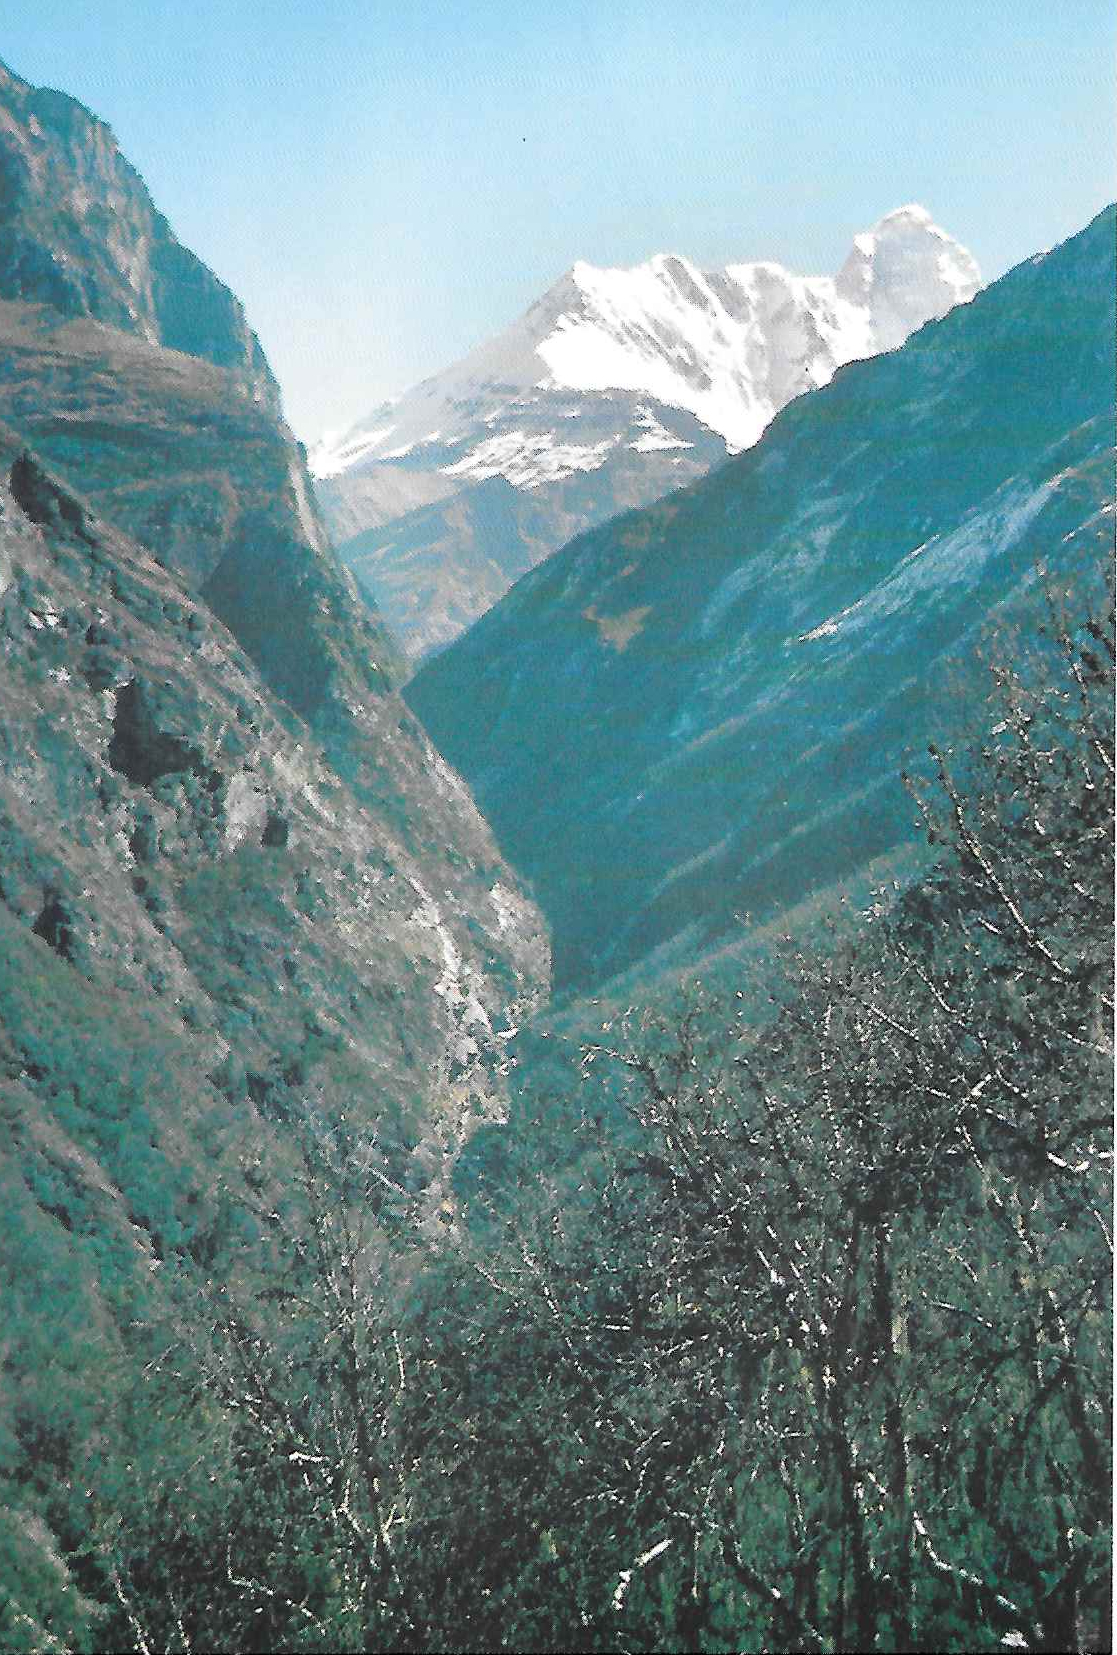
\includegraphics[width=.9\linewidth]{./images/Nanda_Devi_from_Rishi_Ganga.jpg}
\caption{\label{fig:orga300e61}
Nanda Devi from the Rishi Ganga}
\end{figure}

\begin{figure}[htb]
\centering
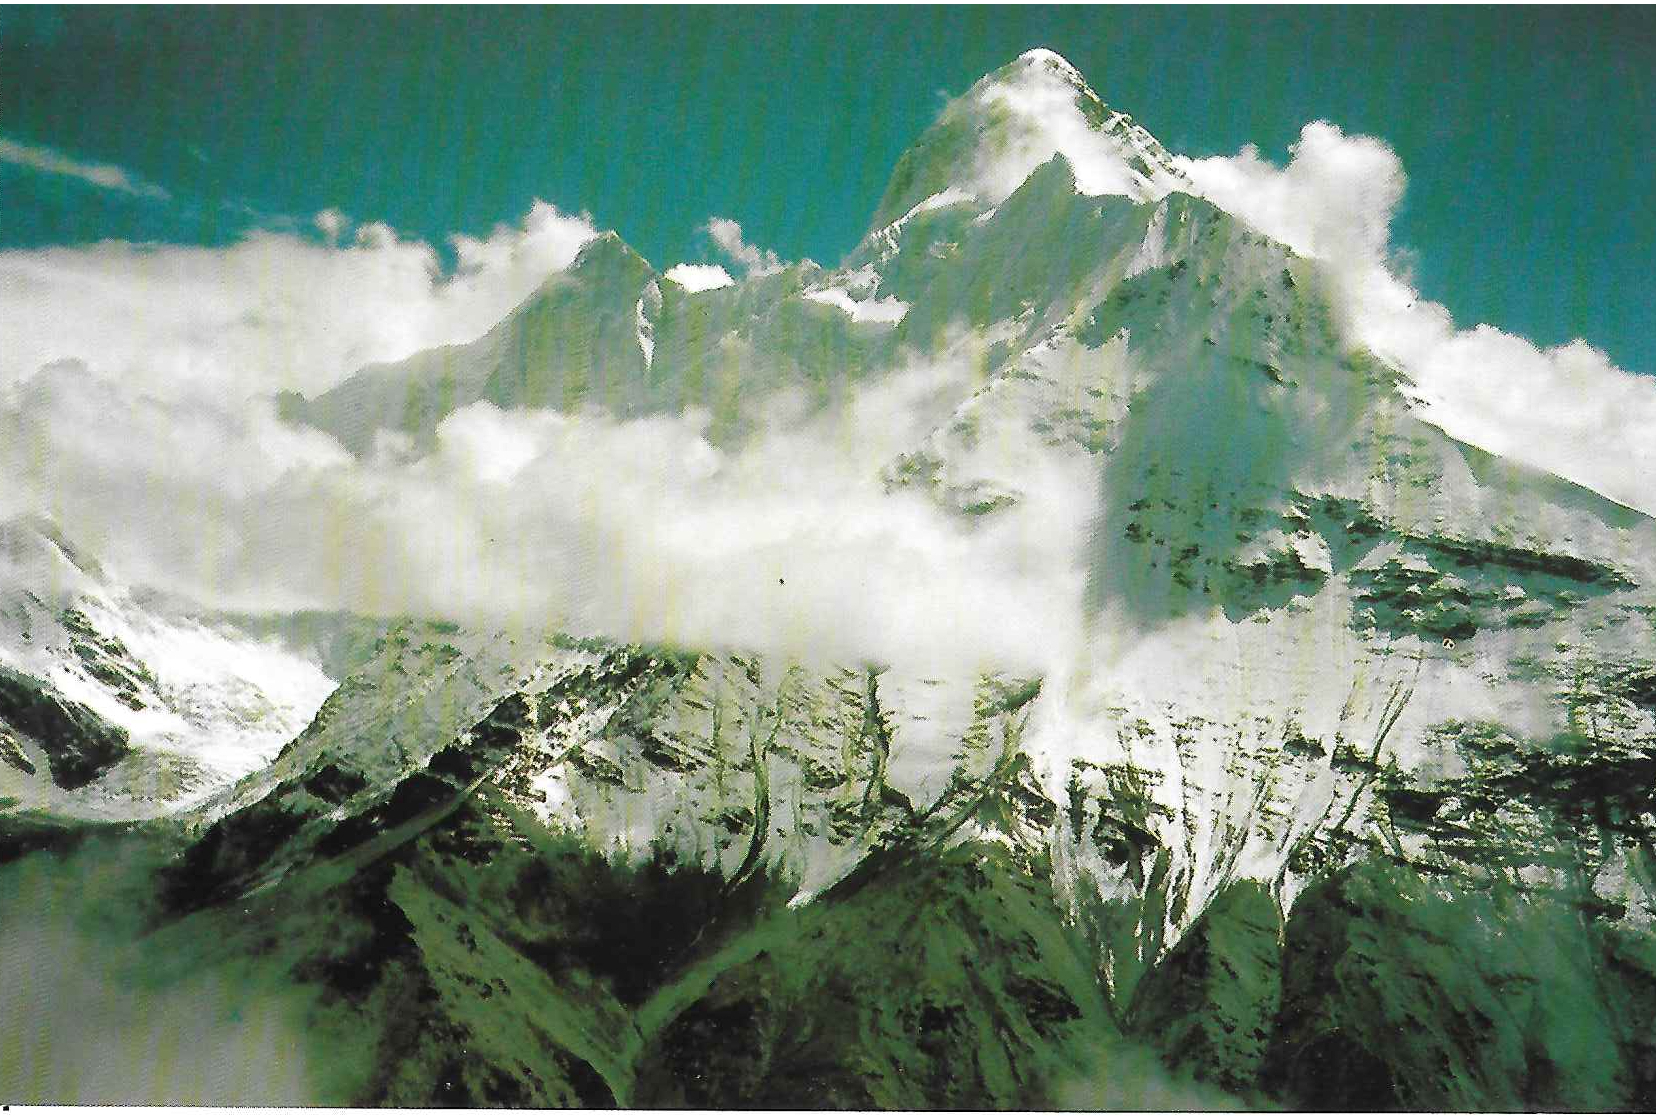
\includegraphics[width=.9\linewidth]{./images/Nanda_Devi_from_within_the_Sanctuary.jpg}
\caption{\label{fig:org5196f16}
Nanda Devi from\(_{\text{within}}\) the Sanctuary}
\end{figure}

\chapter{High Spirits}
\label{sec:orgd2b7d7e}
\chapterauthor{Steve France}

Some years ago, whilst visiting the battle site of Culloden
Field on a damp and misty September day, I was subjected to a
feeling of utter dread.  Subconscious emotions told me, "You must
get away!" People could wander round the graves from clan to clan
for hours but my whole visit lasted less than twenty minutes.  A
year later in the middle of the vast winter landscape of the
Cairngorms, I suffered the same experience.

It was a typical Castle plod, made worse by dense cloud and
deteriorating conditions, but our spirits were high even though
Chris Holmes, Dick Savage and myself felt more at home on rock
than playing the mountain man. The steep slog towards the
Cairngorm plateau was no fun, especially when the skiers were
gently gliding past on the ski tow whilst making sarcastic
comments and giving us sneering looks. Our replies ranged from
"Yes, we do enjoy walking up" to "No, it's not tiring when you're
fit".

Before our language became offensive we saw an ideal
opportunity for one upmanship. By climbing a high banking of snow
at the side of the tow run, we could jump and grab the unoccupied
tow bars!

Weee!\ldots{} up we went and after a short period spent adjusting
the angle of our boots on the snow, a perfect glide was obtained
on our Vibram skis! Protests were heard further down the tow from
"paying" participants and we raised our overmitts in reply  they
could not see the two fingers inside, but I think that the
message was plain enough!

Once over the wind swept edge of the plateau we were on our
own and left to enjoy the beauty of the mountain solitude. The
clouds were white with snow as we came to the col beside Lochan
Buidhe. The mountains merged with the snow into total whiteness,
so bright that our duvets appeared translucent. The silence was
oppressive except for the crunching of the snow. I remember
vividly the way we walked, as if in a slow motion action replay.
This was my first and only "white out", the only reality was
the person in front until suddenly a snow bank resolved itself
into focus in front of my eyes. It was not the snow bank that I
saw but a hole in the snow,  approximately one metre square.
We entered, and as the tunnel opened out, were stunned with
surprise by the ice village which greeted our eyes. It was
without doubt the Ritz of all snow holes with room after room
each connected to the other and complete with its own table,
chairs, raised bed and shelving systems\ldots{} all made out of ice.
It must have been a distant relic from a winter survival course
at Glenmore Lodge but the unnatural silence, together with the
ambient light that soaked through the ice walls, transformed the
shelter into a mortuary of past memories. Imagining ghosts,
goblins and yetis, we ran out of the tunnel and back to the
welcoming "white".

Another mile and our high spirits changed.  I can remember
approaching the final slopes trying to find an excuse to turn
back, but there was no rational explanation why, and so we went
on. The cairn was found quite by accident  we were standing on
it!  because the snow covered all but the brass plaque on top
which shows the various peaks and directions. Even though we had
reached our goal, the summit of Ben Macdui gave us no pleasure.
There was no vista to enjoy, only grey dread and an urge to go
home quickly. The usual summit rest, comprising a bite to eat
whilst soaking in self-satisfaction, was limited to a quick photo
before we legged it back down the mountain.

The campsite talk that night re-lived the arduous knee deep
slush and the "white out", but we never talked about Ben Macdui.
I am sure that strange perception of malevolence was shared
subconsciously between us, although at the time, I never gave it
much thought.

Recently I was reading a book entitled "Scottish Ghost
Stories" and to my surprise, discovered that there is an alleged
ghoul on Ben Macdui called "The Grey Man". Although never seen,
it has been responsible for campers fleeing for their lives,
leaving tents and equipment behind, totally convinced of their
impending doom if they remained there any longer.
Gruesome stuff!

\chapter{Round Edale Walk or "Who Went Where and Who Said What?"}
\label{sec:orgfa07be5}
\chapterauthor{Jack Ashcroft}

An innocent enough walk around Edale.
"You can't get lost up there," was the bar room atmosphere
at half past ten on Thursday evening.
Well you can. If you don't take your map and compass,
whistle, torch, contact lenses   if appropriate  and it's
raining, the cloud banks are low, the gale force on the Beaufort
Scale is approaching eight and you don't check your position
regularly and keep the group together\ldots{}

Ten of us left Mam Nick car park at 8.45 am to tackle the
Walk clockwise. Before Lords Seat the furious Westerly had us
reeling and two returned to the car park. Eight then battled on
for Brown Knoll   a little spread out   but on arrival at the
trig point we were only six in number. We got cold standing there
in the wind, straining our eyes through the mist for the other
two, both ladies. Concern.
    "Secretaries are dispensable."  E

\ldots{}mutter\ldots{}  mutter\ldots{}  mutter\ldots{}  J
  "Let's push off in the true spirit of mountaineering
comradeship."

"Here they are."
Two figures loomed out of the mist. But it wasn't them.
"We haven't seen them    we followed the path all the way."
So we were eight again, but a different eight.

"Hope they are together."
  "She's never been up here before   hasn't got a map."  E
  "She knows the topography   she's got common sense."  E

"Your decision."
  "Let's go on and see what happens."
We walk on to Edale Cross.

"They're here."
"You're disqualified   missed out Brown Knoll check point."

"Rubbish, we followed the right hand side of the dyke.
Pointless going off route to the trig point."
  "We really will keep together now."
And we basically did\ldots{} to the shelter of the boulders below
The Pagoda.

"I've just been talking to someone up there who I
thought was one of us until I pushed my nose into his
face."
"We need a Kinder sixth sense move to the top of
Grindsbrook. We'll stop there for a bite to eat."
"OK, it's alright. Don't bother to get your map out."
So ten set swiftly off into the wind, rain and mist, full of
confidence.

"It's rough going. Too much up and down the groughs."
"Stop. Let's think where we are."
"More to the right."
"Up to the left."
"We've lost them now."
Five of us left.
"Let's stick together."
"The stream is going north. This must be the Kinder
River."
"This way."
"Move south."
"No. Move over. Still more east."
"It's like caving above ground."
"Drop into the groughs at the head of Grindsbrook."
"This is it."
"Damn! It's Crowden Brook, not Grindsbrook."
"We've gone round in circles."
"No we haven't! Just a horseshoe   a mile to progress
half a mile."
"Are we stopping to dry out tights and long johns?"
"I wear socks the same as every one else."
"The feminist touch."
"Right, now for Grindsbrook, I bet someone's there."
Someone was.
"I've been here five or ten minutes. Dropped into the
groughs head of Grindsbrook on a compass bearing. I
haven't a map."

It was 12.38 pm.
    "Don't go down there. It's best to wait until we get to
Golden Clough if you want to go down."
Six of us stood at the top of Golden Clough.
    "Who's for going down?"
    "Well\ldots{}"
    "Tea in Coppers."
    "Newcastle Brown in The Nags."
    "You can tell who are the walkers!"
    "You can tell who are the climbers!"
    "Who's doing what?"   "That's it then."
Two went down for refreshment. Four went on. Too swiftly again, I
fear.
    "We haven't seen the trig point."
    "It's over there."
    "This is the head of Jaggers."
    "Doesn't seem deep enough to me."
Neither was it.
    "That's the Snake road down there and we are walking
out."
    "It's Blackden."
    "Turn around for Crookstone Knoll."
    "I'll watch her down there and you up here   keep in
contact."
    "You can get off the plateau but you may be fifteen
miles from where you want to be."
And so off the plateau towards Crookstone Barn. Two lasses and
two lads.
    "Those trees must be two of the toughest in the Peak."
    "Down the Roman Road to meet the car at The Cheshire
Cheese."
    "There's a quicker route than that."
    "Oh! Someone has moved the fence."
And so we were on the road at Edale End. The two lads approached
Lose Hill under the railway near Fiddle Clough. It was 3.20 pm.
The two lasses walked along the road to meet their transport at
The Cheshire Cheese.
Lose Hill wasn't in fact traversed by both the lads: one
followed the track around the south side of Lose Hill into the
wind. Slow tiring progress.
    "I waited here out of the wind so we'd be together to
traverse Mam Tor. It looks vicious up there."
And so it was. Racing cloud touching the summit, the light
gone, crawling on hands and knees. It was 5.05 pm. The rest of
the cars had gone.
    "I've never been in wind like that before."

And who sheltered at Kinder Downfall for lunch and never saw
Crowden Brook or Grindsbrook at all? What a Who dunnit! Oh the
freedom of the hills! u  I call an EGM. The motion:
"The CMC should affiliate to the British Orienteering
Association."
Proposed   Guess Who?
Seconded   Get Lost! Plus ten supporting Kinder members.

\chapter{Rhinogs Meet}
\label{sec:orgdbda051}
\chapterauthor{Frank Mellor}

Arriving at Dinas Farm in the early evening of Friday I was
surprised to see Sean, Mel and family already prospecting for a
good pitch. We had pinched an extra day to climb on Tryfan and
although we had stopped in Beddgelert for a beer with Dunk, I had
expected to be first at the campsite.

"Evening Sean, not been hanging about then?"
"No, we got off early and had a good run down. Had a good
day?"
"Aye, we've done  Grooved Arete . Bit nippy on the fingers but
a great route. Nobody else here?"
"Not seen anybody yet. Nice spot this. I think we'll get
settled and put a brew on."
"OK Traverse tomorrow? Weather looks promising."
I put up our tent a fair distance from Sean's as I wasn't
certain how young Pete would react to his first night under
canvas. After lamb chops it was nearly dark  after discussing
transport arrangements it  was  completely dark  and after drifting
off to sleep for five minutes it was light again! Car headlights
illuminated the canvas. Dave and Jenny with Andy and Rosy.
"Hey Frank, doing the Traverse tomorrow?" Andy wanting to
get it sorted.
"Yep. Wake you up at six."
"Six? Bit early, in't it?"
"Yeh, but Sean's keen not to be late back and Mel's going to
come and pick us up."  Always blame somebody else!
"OK then."
Drift off back to sleep again. Ten minutes later   same
performance with Vanda. Anyway, now everybody knows.
Half past five, alarm goes off. Damn thing's somewhere under
the flysheet. By the time I've struggled with the zip it's
stopped ringing. Bash it one anyway. Start a brew and leave it to
Jennifer. Stick head out   lovely! Sun coming up and pale blue
sky. Over to Sean's tent and whisper   instant reply. Over to
Andy's   nothing. Try again but this time stick head round flap.
Now there's a bit of snorting and the bag starts to move.
Suddenly the top half of it rears up and out pops a bleary eyed
face.
"Andy. It's six o'clock."    "Yes I know. I was just waking up. You needn't have
bothered."
As if this isn't enough I get a withering glare from Rosy
out of the gloom at the back of the tent. I sure wouldn't like
this job every morning! Vanda's reasonably civil though and Colin
manages a muttered reply. That's everybody. Dave and Jenny are
doing a slightly different walk and, knowing them, they've
probably been gone an hour already.
Whilst having a cuppa outside the tent I hear the first
cuckoo of the year and a few minutes later a heron flaps over.
People are emerging, gathering rucksacks, pulling on boots,
sorting out gear. Should be ready for off soon. Wait a bit
where's Colin?
"Anybody seen Colin?"
Nobody has. The beggar's gone back to sleep. He's eventually
persuaded out and we're off in two cars round to Trawsfynydd.
We park just off the track up to Cefn Clawdd, at an old
quarry site. We're walking by 8.15 am. Not bad considering we'd
been aiming for 7.30! We go up over wet ground, finding and then
losing a track to join the ridge just east of Diffwys. It's warm
work and pullovers are soon shed. On Diffwys it's cooler.

Roughish going with detours for crags and deep rocky trenches on
the way to Ysgyfarnogod  Sofarso good . Now "The Celtic Badlands"
and Clip. Much cooler now and the strongish breeze is blowing
clouds of May blossom up from the valleys. Strange how its petals
melt when they touch the skin. Elevenses on Clip. Ratatouille for
Vanda, cheese butties for me. Craig Wion is tough going but the
weather is being kind. Snowdonia is getting it and we can see
fresh snow on the Arenigs, but we're in the clear apart from the
occasional flurry of blossom. I'd like to have a beer with Dunk.
The way is barred again by rock walls and trenches.

Profanities from unexpected sources accompany our passage. Only
the graffiti on the rock walls forces the realization that we've
made it to the Roman Steps. Lunch on the big Rhinog! Easily up
after an awkward first couple of hundred feet. Past Llyn Du and
into sunshine on the long shoulder leading to the summit. A small
group of backpackers is just leaving. A nice rest there. Quiche
Lorraine for Vanda, pasty and Guinness for me. I'd like to have
another beer with Dunk!

Those who've been here before assure us that we're
psychologically over half way and that there are paths over the
remaining ground. Ten minutes later we are hearing that there is
no reason why an apple shouldn't fall upwards from a tree.
It's    something to do with statistics. One thing's for certain. There's
a helluva dip between Rhinog Fawr and Rhinog Fach  it feels like
sea level in Bwlch Drws Ardudwy.

There's a difference of opinion at the Bwlch. Colin and
Vanda go up past Llyn Cwmhosan and the rest of us go straight up.
We give it some fettle and get there first. Colin's not long, but
arrives with the news that Vanda is missing this one out. We
catch her up just past the imposingly situated Llyn Hywel. Y
Llethr is the biggest hill of the day but doesn't feel it, the
going is better. There are grassy paths. Apples do fall upwards.
The pace quickens up to Diffwys. The evening sun delineates the
majestic north face of Cader Idris. What a tremendous walk! We're
dropping from the south west ridge of Diffwys to the col. Over
Craig y Grut to Bwlch y Rhiwgyr to Sylfaen, to Mel waiting with
the car and lastly to the fleshpots of Barmouth. Fish and chips,
beer at last with Dunk. The atmosphere is great!

As we sit drinking, the dreadful thought occurs to us that
the pub may be closed tomorrow  Sunday . We ask the landlord who
confirms our suspicions. Andy returns from the bar.

"It  is  dry tomorrow, Andy," says Rosy.
"Oh, have you heard the weather forecast then?" asks Dunk,
waking up\ldots{}
Unfortunately it  is  wet. Steady rain that doesn't look like
stopping. Ian has arrived. We cheer him up by telling him what a
good day he missed yesterday.
It's a late start. Vanda's due back in Sheffield but the
rest of us drive to Barmouth and pay 12p for a walk across the
toll bridge. At the other side first Colin and then Dave decide
it is not worth it. Colin goes bird watching and Dave goes to dry
out, having discovered his anorak isn't waterproof. The dwindling
party plods on.

Jennifer insults Ian by telling him he'll be the next to go.
It works. He stays. We follow the disused railway along the south
side of the Mawddach estuary to Penmaenpool. The rain lashes our
backs.

Lunch in the shelter of the pub  it  is  closed . Over the
toll bridge to Borthwnog. Only 1p this time. The rain has stopped
but there is a strong drying wind.

Pleasantly up through the woods to Garth gell. A jay hops
across the path. A squirrel scampers ahead. We link paths and
forest tracks back towards Barmouth. It showers on and off. We
put anoraks on and take them off    and on and off.
We finish at Barmouth's Panorama Walk. A commanding view up
the estuary and out to sea. Cader's hidden behind the clag. Back
in town, Colin and Dunk are dozing in Dave and Jenny's car. We're
back and dry.

The evening passes by as meals are cooked, then there's
chatting outside the tents in the gathering gloom until it's too
cold for comfort.

Monday morning. Grey and unsettled. Tops look likely to be
cloudy. The Kimes suggest the Berwyns. No one objects, so it's
down tents and off to Llandrillo.

A pleasant spot this: a spired church and an elegant bridge
over a fast flowing river. A gentle path leads up onto the broad
ridge where we stop for a bit near the "Wayfarer" plaque. The
clouds have rolled away and although it's still overcast, there's
no rain. A strong breeze makes us don cags for the ridge up to
Cadair Bronwen. The long ridge rolls us on to Cadair Berwyn and
Moel Sych where we turn north west and head back over marshy
ground toward the valley. Lovely warm sunshine welcomes us back
to the village.
Our weekend in Wild Wales is over.

\chapter{A Brief Look at Lahul, Zanskar and Ladakh}
\label{sec:org582c71e}
\chapterauthor{Jack Ashcroft}

If you glance at a map of the Himalaya, extending across to
the north of India, it is approximately 900 miles between Godwin
Austen  K2  in the Karakoram and Everest in Nepal   much the same
distance as from north to south of The British Isles. The terrain
of the landscape contrasts vividly in both cases, but the tract
of country between K2 and Everest is the greatest contrasting
landscape in the world  it ranges from tropical forests to
mammoth rivers and contains the  world's highest snow  and
ice clad mountains from which issue the world's longest non polar
glaciers. It also includes the high plateau desert landscape that
characterises the country of Ladakh, close to the Karakoram.
Ladakh is a very dry area, as indeed is the Karakoram itself.
However, the mountain peaks of both Ladakh and neighbouring
Zanskar rarely reach 7,000m whilst those of the Karakoram exceed
8,000m, giving that little extra precipitation.

If you wish to visit the Himalaya during July and August,
the areas of Ladakh, Zanskar and the adjacent province of Lahul
and Spiti are the places to plan for. The further east you go
towards Nepal, the more rain you can expect in the monsoon
period.

Enough of this meandering introduction  suffice to say that
with August our only choice of holiday, Harry Woods and I planned
a trek in 1982 through the Zanskar Valley from Lahul to Kishtwar.
We covered 180 miles in just under three weeks over the Shingo La
 5,096m  to Padam  3,600m , the capital of the Zanskar Valley and
then out again over the Umasi La  5,300m   an eight day trek of
contrasting terrain, from the desert like landscape of Zanskar
through lush green forested gorges down to Kishtwar.

General Bruce, having reached a 20,000ft summit to the east
of the Shingo La in 1912 wrote:
 "Zanskar to the west, though bare enough  compared to his
view east  in all conscience, is wild, broken and savage to a
degree  a more inhospitable country it would be hard to find  but
some of the peaks are fine and boldly shaped\ldots{} the great
difficulty in Zanskar\ldots{} is the number of streams to be
negotiated\ldots{} its intense savageness attracted me."
He goes on to say that the people who live there must be
very hardy and able to withstand great cold.

It is this country one enters on the ten day trek from
Darcha, the police post in Lahul, to Padam. Our trek also
included a diversion to visit Phuktal, the most impressive
monastic site in Zanskar. Bruce pointed out that the country is
"wild and broken"   but that the people are reasonably kind and
interesting, inhabiting the highest settlements of any size in
the world.

Kargiakh and Thangso at 4,200m over the Shingo La have no
doubt been the frontier posts between  Zanskar and Darcha for
thousands of years and only recently has the policing stance been
eased. This is indeed a dry and bleak environment, certainly the
most spartan I have encountered in my three visits to the region
but welcome after the three day trek through the virtually
uninhabited country from Darcha and its many "streams to be
negotiated".

Michel Peissel, an anthropologist much travelled in the
Himalaya, gives good insight into the Ladakhi character. His book
"Zanskar   the Hidden Kingdom" is a very readable description of
a walk through Zanskar, only two or three years after Ladakh was
opened to tourism, the borders having been closed by the Indian
authorities from the end of the Second World War.

There is much to write about in nearly three weeks travel
through these ancient sparsely populated valleys, but suffice to
say that it was a pleasant relief and a revelation to walk into
Padam having followed wild and broken gorge after gorge for over
a week. Padam, with its population of a thousand or so, is the
capital of Zanskar   effectively half way along a hanging valley
some eighty miles long with oasis like settlements surrounded by
mainly dry, barren, mountains. The only ways out lie over passes
of some 4,000m to 5,000m to the north, south and west. To the
east is the outlet of the Zanskar River, not a feasible route in
summer, we were told, but in winter becoming a hundred mile
frozen highway giving access from Padam to Leh  the Capital of
Ladakh  and the confluence with the embryonic Indus far to the
north. Peissel's description of Zanskar   "The Hidden Kingdom"
is indeed an apt one.

We stayed in Padam for two days and then set out on our
eight day trek over the Umasi La to Kishtwar and Kashmir. The
Umasi La is a more serious pass than the Shingo La and is
surrounded by interesting peaks. It had been our intention to
camp for two nights high on the pass with a peak in mind but this
was not to be. We climbed to the pass near the summits but only
stayed for twenty minutes as the weather was blowing in from the
valleys of Kashmir. We resolved to get down the glacier on the
far side as soon as possible rather than camp high, an hour's
descent through jumbled ice falls and moraine snow in poor
visibility.

What were the highlights of our trek? Perhaps "highlights"
is the wrong description, but the contrasting temperatures in
Zanskar certainly come to mind   from one hundred degrees
fahrenheit at high noon to below freezing at nights  the Buddhist
culture in Zanskar and the contrasting Moslem culture down in the
valleys of Kishtwar  the unclimbed peaks of considerable interest
around the Shingo La and Umasi La, not too huge and clustered
more dramatically above the Umasi La  not to mention crossing the
streams and keeping the party together! On our approach to the
Umasi La we managed to end up with Harry and I on one side of a
glacier snout and melt waters  quite extensive at seven o'clock
in the evening  and with our porters, tentage, food and sleeping
bags on the other side. Our lot was a forced bivouac at 16,000 ft
at the side of a crumbling glacier snout with thoughts of snow
leopards, until the dawn arrived and we eventually found our way
through the jumbled terrain to our two porters and a welcome
meal.

It was a fine trek. We were a little austere in our planning
with a very basic diet and at the end of three weeks it certainly
felt as though some energy had been expended! The weather was
kind with only one and a half days of poor weather in eighteen
unluckily the one poor day was the day we traversed the Umasi La.
In 1984 Harry and I were joined by other Sheffield based
climbers for another visit to Ladakh. This time eight of us
travelled out to India at different times in July and August to
meet up in Leh some sixty miles north of the Zanskar valley. The
fact that we managed it at all was remarkable, as Kashmir and
Punjab were not in a very settled state at the time and we had
made contingency plans to go further east to the Garwhal if Leh
proved inaccessible. Despite having travelled out in four
separate groups, all eight of us  including Frank and Jennifer
Mellor  met up in Leh during the first week of August for a trek
in the Marka Valley.

I can thoroughly recommend the Marka Valley as an experience
in gentle Himalayan travel, certainly the way we did it and
particularly in contrast to our trip of 1982. Taking advantage of
the tourist office facilities in Leh, we took with us an Indian
Mountaineering Foundation Guide and two horsemen. The Marka
Valley trek is a regular summer tourist route of some seventy to
eighty miles, a round trip from Leh which crosses two passes, the
Ganda La  4,450m  and the Longmaru La  5,220m . From the Ganda La
we had a rather hazy view north west to the Gasherbrum K2 massif
and south to the Kishtwar peaks. We had planned a trekking peak
ascent which turned out to be a sortie into the Kang Yissay
group. We established base camp at about 5,000m in an idyllic
situation and attained the north summit of Kang Yissay  6,090m
and a subsidiary point La Ribla  5,960m  on the opposite side of
the Kang Yissay glacier from the principal peak.

We were eighteen days on this trip including four at base
camp. The highlights of the holiday were many. Leh, being the
capital of Ladakh, has a military garrison and is on the
centuries old Karakoram Pass trade route between Tibet and India
it is more in touch with twentieth century living than Zanskar.
Nevertheless, three of us are fairly convinced that we saw   and
I've got to use the expression   a  "Yeti like creature" leap over
the boulder strewn slopes of Kang Yissay at five o'clock in the
morning soon after we had left base camp on our eleven hour day
on the peak. Our first impression was reinforced later when we
failed to recognise the species on referring to the flora and
fauna of the region on our return to Leh.

The Hemis Gompa, some three hours by bus from Leh, is a fine
example of Buddhist architecture some five hundred years old.
Even better is to walk 1,000 feet above Hemis to the tiny
sanctuary of Goatsang where the Lama regularly scrambles up Grade
IV rock routes to maintain the prayer flags that span the valley.
Hemis is the centre of the Buddhist festival held each year in
May after the winter snows which cut off the valley from October
to April have receded to allow thousands of pilgrims to visit
Ladakh.

This article hardly does justice to our visits to Ladakh in
1982 and 1984. I quote from the pre war writing of Dr. Tom
Longstaff:
"Walk for a week or ten days from Simla along the Hindustan Tibet 'road'
make a camp in the first valley south of the
Satlaj that takes your fancy: from here climb all the peaks on
both sides of the valley and you will have had as much good
climbing as in an Alpine season and for the same expenditure, if
your party consists of not more than three good climbers who can
muster enough Hindustani to do their own job for themselves. Here
is both pleasure and high mountains. The scale is bearable: on
the giants is only labour and weariness: they are best to look
at."    I would not argue with this, but I am sure that I do not
need to remind anyone of the necessity for fitness before
getting to altitude, followed by a sensible period of
acclimatization. After that, the usual medical precautions to
fight the stomach microbes on a short holiday in India are
essential for both "pleasure and high mountains".
As a postscript, do study your logistics. We were a little
short, to say the least, on our porterage when crossing the Umasi
La in 1982. If our two porters had not been prepared to carry
such heavy loads we would not have made it over the pass, and as
a result of their heavy loads, they fell behind on the ascent and
we ended up on opposite sides of the glacier snout that August
night in 1982.

The mountains of Ladakh are many and varied, most of them
awaiting first ascents. Once one moves north over the passes of
Kulu, Chamba and Kashmir one enters a new world   "Little Tibet"
as it has often been called. It is a pocket of high plateau where
India meets China in both the geographical and political terms of
today. The area has never been released from the tensions which
existed in the post war period and it now needs care in its
future development, particularly in relation to tourism. The
signs of rapid progress are already there and I hope that the
mountaineering fraternity will observe the rules.
Have you purchased your "Ladakh Zanskar" guide book yet?
\begin{figure}[htb]
\centering
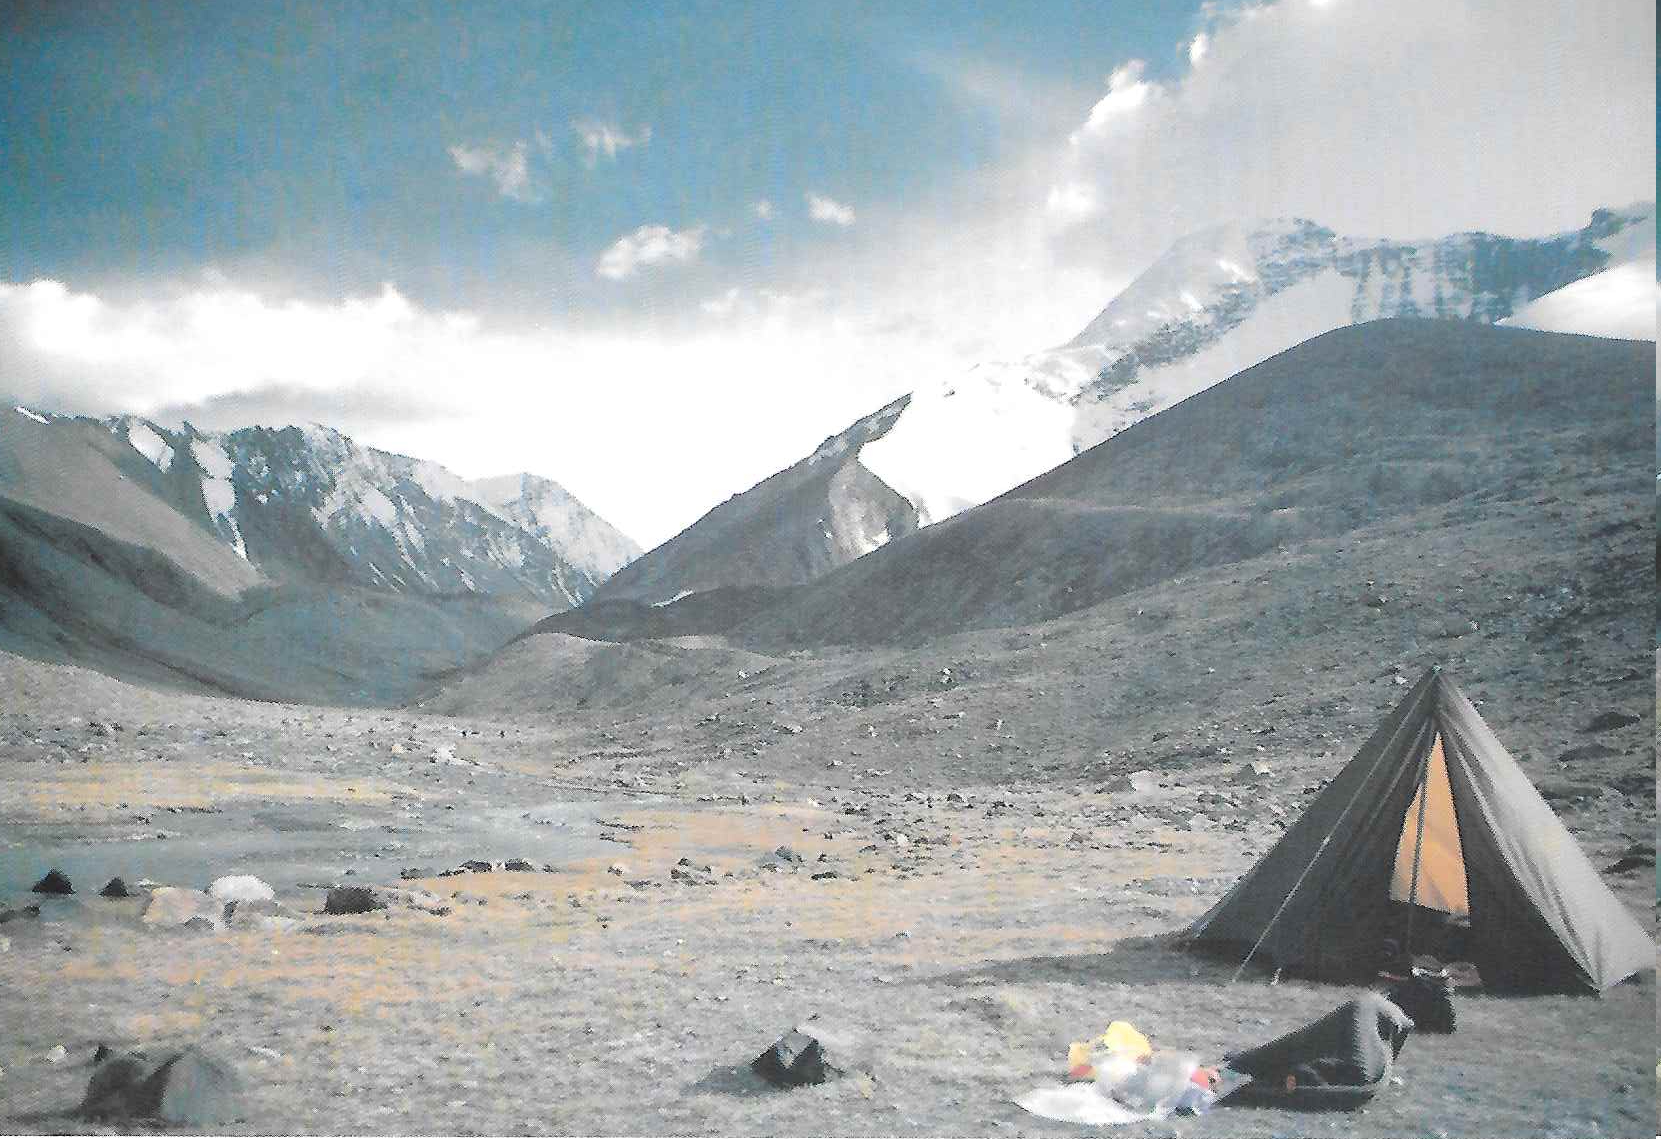
\includegraphics[width=.9\linewidth]{./images/Base_camp_below_Kang_Yissay_Ladakh.jpg}
\caption{\label{fig:orgcb02ee5}
Base Camp Below Kang Yissay Ladakh}
\end{figure}

\chapter{Bamford Edge}
\label{sec:org975cde5}
\chapterauthor{Jennifer Mellor}

It was all happening at Bamford Edge on Sunday. Club climbers hard men
from seventeen to sixty seven were out in force. The weather was warm
and fine, the rock dry and everyone keen to get to grips with the
climbing after the winter. I counted a fair number of Club members,
friends and associates and I hoped that Mr Darwent, the keeper,
wouldn't come and check. His letter had said that he would stretch the
normal six climbers at any one time "a bit", but I doubt if he really
meant to go quite as far as twenty seven! The hard men were of course
doing things which looked impossible some of us lesser mortals only
just managed Possibility .  A35 proved a popular route and lunch time
was enlivened by various attempts to start a climb next to Kelly .
This involved swinging on one hand and trying to put one's right foot
in one's right ear! One superhuman actually managed this feat without
a rope in green pyjama bottoms, what's more! It certainly had the
cameras clicking. This was a new fashion for "proper" climbers that
season and I was told that girls would be allowed to wear baby doll
style, if only for Extremes!

After lunch we all relaxed a little, now that the mobile audience
otherwise known as "The Symbolic Mass Trespass" had passed on. Coming
over the top to face hundreds of "protestors" eating their butties had
been more harrowing than the climbing.  Most people gradually drifted
towards Gun Buttress, doing climbs on the way, and the afternoon
finished with some pleasant easy soloing on the shorter routes at that
end of the Edge.  We went home tired and happy after the kind of
Sunday one dreams about in the depths of winter.
\begin{figure}[htb]
\centering
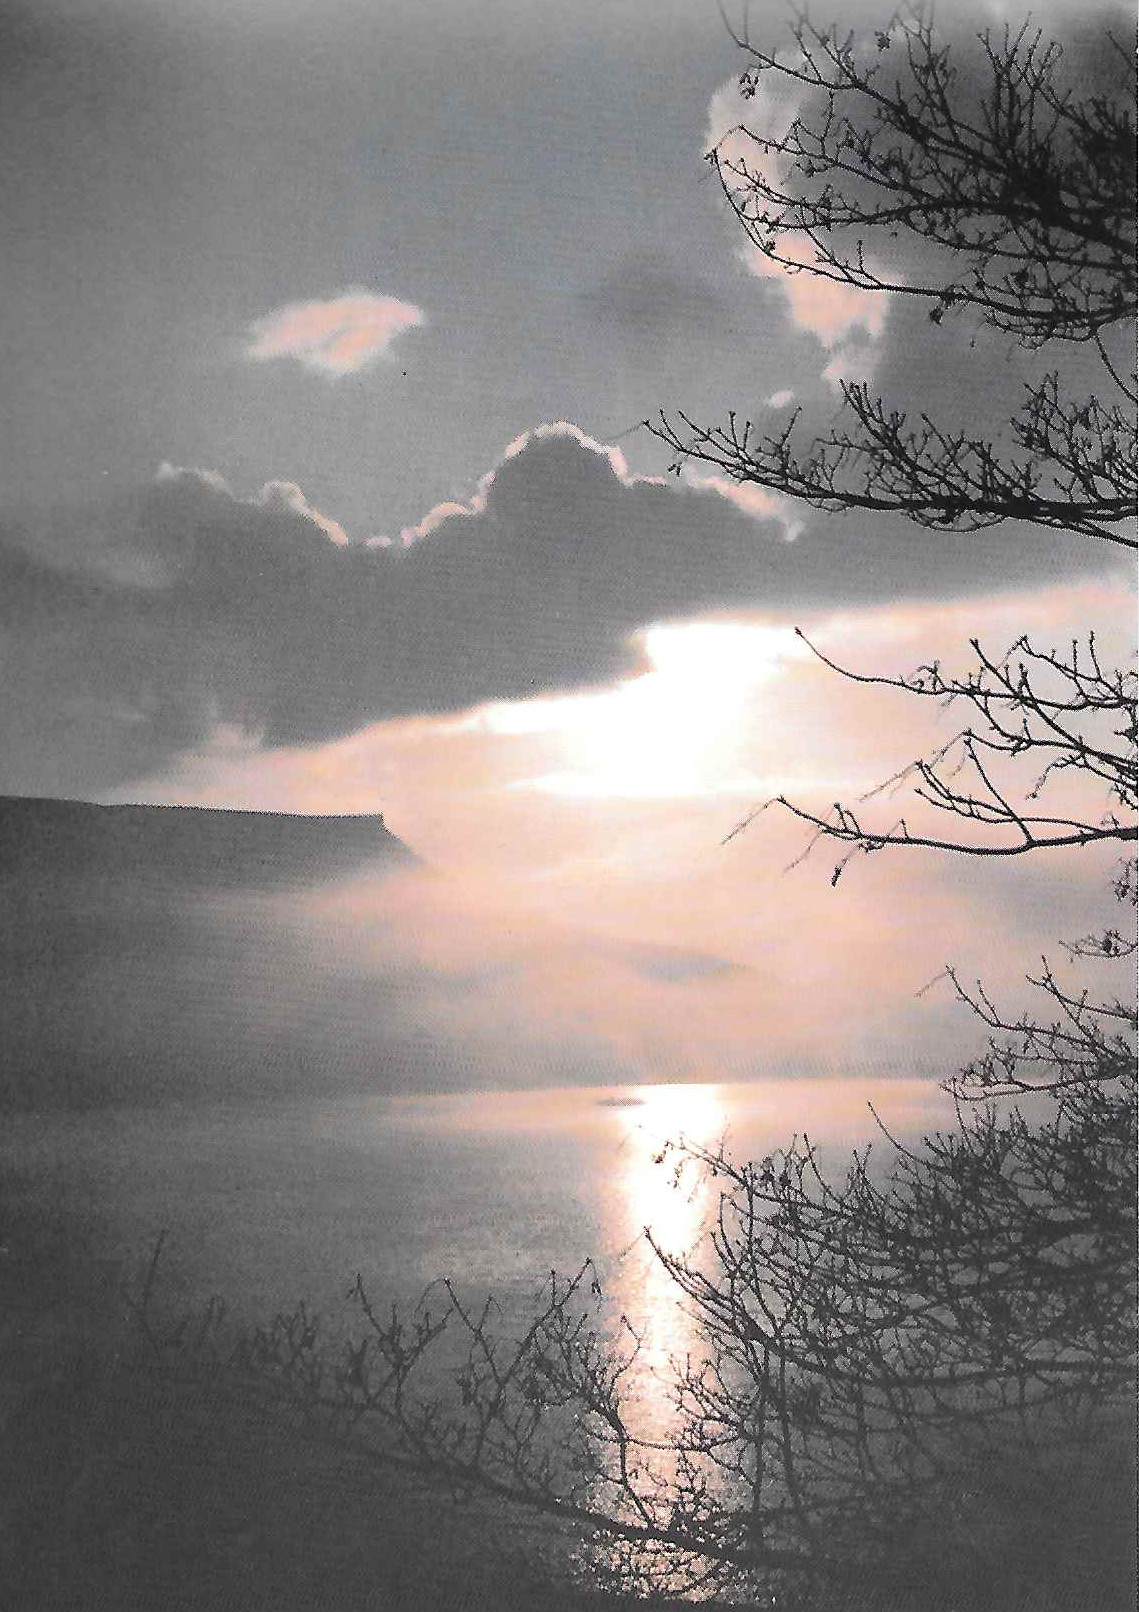
\includegraphics[width=.9\linewidth]{./images/Bamford_Edge_from_Ladybower.jpg}
\caption{\label{fig:orge1c1de0}
Bamford Edge from Ladybower}
\end{figure}

\chapter{Boat Trip to the Western Highlands}
\label{sec:org1192d67}
\chapterauthor{Mike Jackson}

It was July 1983, time at last for our long planned visit to
the "Rough Bounds" of Knoydart, especially significant for Jim
Thomson since he was to complete his Munro trail in this remote
and beautiful area. My old friend Bob Madeley, armed with a
yacht master's certificate, had chartered a boat at Loch Carron,
a little twenty nine foot beauty named "Jackie", providing the
ideal approach to this wonderful district of long narrow sea
lochs and dramatically wild hills. The party from Sheffield
included a friend David and my son John and we stayed overnight
in Edinburgh with Jim and his wife Jean, much appreciating their
warm welcome and kind hospitality.

On the Saturday we drove up to Lochcarron village and cast
off from the old ferry slip way at North Strome at 5.00 pm on a
bright and sunny afternoon. The calm waters of Loch Carron
glistened in the sunshine and we enjoyed an evening of dark blue
sea, clear blue sky and exquisite beauty with a magnificent
panorama across the sea of the sharp serrated skyline of the
Cuillin of Skye. The trip was enlivened by many sightings of
seals, eiders and guillemots and after negotiating the narrows at
the Kyle of Lochalsh we moored at 8.00 pm in Loch na Beiste south
of Kyleakin, a backwater of idyllic peace and tranquillity with
herons and gulls calling and curious grey seals around the boat.

We set off for Loch Hourn at 5.00 am in order to pass
through the narrows of Kyle Rhea on the tide, our main objective
of the day being to climb Ladhar Bheinn, the grand hill
overlooking Barrisdale Bay. After passing the Sandaig Islands
with a view behind of the Skye Cuillin, the boat turned towards
Loch Hourn and we looked inland to great misty hills with magical
light effects on the peaceful waters. Three cormorants adorned
the buoy at the entrance to the loch, arctic terns flew by
regularly and later a golden eagle soared effortlessly over
Barrisdale. We anchored on a beautiful morning in sheltered Poll
a'Mhuineil two miles west of Barrisdale. Bob and John stayed on
the boat but David, Jim and I walked along the shore above the
blue waters and met our friend David Howgate who had walked in
from Kinloch Hourn the night before to camp by the outflow of the
Coire Dhorrcail stream. This was a lovely campsite at which to
linger, with foxgloves in flower by the stream and with a
splendid view over the loch to Beinn Sgritheall, but the clegs
were out in force and encouraged us to set off up the hill.

The walk up the ridge east of the coire, deeply incised in
its lower reaches, was enjoyed with frequent pauses to savour the
exquisite views of Loch Hourn. We traversed steep grassy slopes
to join the fine stalkers track which comes up from Barrisdale.
We could now see right down to the loch and over to Beinn
Sgritheall whose high summits were just visible above a great
bank of white cloud, the scene framed by silver birches. As the
track led into the coire to join the lovely stream with its
cascades and pools, our sight of the sea was lost but the crags
and gullies at the head of the coire became visible with patches
of beautiful white mist hanging about them. As usual in high
summer, innumerable orchids and bog asphodels were growing in the
lush green grasses. We headed for the steep grassy slopes to the
right of a great rocky promontory, with fine views of the
impressive ring of high crags supporting the indented ridge
overlooking the coire. Higher up the steep slopes we came across
clumps of pink thrift and numerous white flowers of the starry
saxifrage.

We arrived gratefully at the narrow col on the ridge and
turned up the next section, steep in places and with a charming
thrift garden adorning the way above the cliffs of the coire.
Then on to the narrow East Summit of the mountain with a view to
the south which was grassy, green and wild rather than beautiful
and with a glimpse of Luinne Bheinn beyond the dramatic end of
the ridge we had climbed. From the cairn we could see down into
wild and rough Coire Odhar but the walk along the delightful and
airy summit ridge past the Ordnance Survey cairn to the west end
of the hill brought us into a wet mist and the wind became very
chilly. We hurried back to the East Summit and turned down the
ultra narrow and steep sided ridge on the north side to a minor
col and then up to Stob a' Choire Odhair, a further delightful
section of the walk, albeit still in the mist.

After coming some way down the north east ridge we suddenly
emerged from the mist with a fantastic panorama of Barrisdale Bay
and the narrow upper reaches of Loch Hourn. Across the great
depths of Coire Dhorrcail, the steep buttress of Stob
a'Chearcaill protruded grandly and impressively from the mist.
This was indeed a wonderful viewpoint and whilst picking our way
down the ridge over a number of steep and awkward sections we had
entrancing vistas at every step. David H. headed back to
Barrisdale and the rest of us left the ridge to return to the
boat down steep and broken slopes of long grasses mixed with
rocky outcrops   a real taste of the "Rough Bounds"! We later
picked up David at his campsite before sailing through the
narrows and eventually anchoring near Skiary at the head of Loch
Hourn, a most dramatic and exciting location at which to spend
the night, the loch hemmed in by steep hillsides towering above
the boat.

The next morning was peaceful and quiet but with grey mist
on the slopes above the loch. After being ferried ashore we
followed the delightful lochside track to Kinloch Hourn, a
wonderful place having a unique atmosphere of serenity and quiet
beauty, with wavelets lapping quietly against the edging of brown
and orange seaweeds, the calls of sandpiper and common gull, and
the arctic terns hovering and then plunging into the placid
waters. The mist cleared from the summit of Sgurr a'Mhaoraich
from which we had enjoyed fantastic views down to the head of the
loch some years before. We then returned to the boat for the next
stage of our journey to Loch Nevis and our remaining Knoydart
Munros.

During the sail back down the loch, Ladhar Bheinn massively
overlooked our position, a magnificent combination of great coire
cliffs and steep supporting ridges. At Barrisdale, a pair of red
throated divers took off and wheeled around the boat. We later
enjoyed a magical sail through the Sound of Sleat with numerous
shearwaters trailing their wings just above the waves, family
groups of guillemots on all sides and a solitary gannet plunging
into the sea. The weather steadily improved as we came into
Inverie Bay with Sgurr Coire Choinnichean towering steeply above
the settlement and a long view to remote Sgurr na Ciche at its
sharpest, a delight of blue sky and sea with white clouds above
green hills and the sun gloriously warm and bright. After a brief
halt we sailed on through the narrows of Kylesknoydart and
eventually moored the boat by Eilean Maol offshore from Camusrory
at the head of the loch. This was a glorious evening with a
magnificent view from the boat up to the acute and shapely
pyramid of Sgurr na Ciche and the rocky heights of Ben Aden,
right in the heart of Knoydart. The weather seemed set fair for
our next day when we hoped to enjoy with Jim the last two Munros
he had still to climb.

The following morning was misty and grey, and as the dinghy
ferried us to the shore at Camusrory a heavy drizzle set in. We
walked on to the ruins of Carnoch where the nearby river
 notoriously difficult to cross hereabouts  was so low that it
 could have been forded easily at a number of places  in any
event, there is now a footbridge near Carnoch and those purists
who object to it can still avoid it if they so prefer. The Mam
Meadail track rises in a series of well constructed zig zags,
much appreciated by most but which caused Jim to express
reservations as to how much additional distance was incurred by
following them! The drizzle soon stopped and although Sgurr na
Ciche remained in the clouds there was a clear view back down to
the colourful saltings of the River Carnach, the yellows, oranges
and browns contrasting beautifully with the green grass and grey
rocks of the surrounding hills. The air was filled with the
fragrance of the bracken and bog myrtle and as we were all
wearing shorts the long wet grasses merely freshened our legs.

Once at the bealach we could see right down Glen Meadail to
Inverie Bay and over to the distant and hazy Skye Cuillin. A
steep climb up broken slopes brought us to the south east ridge
of Meall Buidhe which led directly to the South East Top. By now
the clouds had cleared from the summits to give magnificent views
over this great wild area, in particular towards the Sgurr na
Ciche to Sgurr Mor ridge which I had traversed with Jim, John and
Andy Smith the previous year. There were also grand views across
to Luinne Bheinn beyond great expanses of ice scoured grey rock
in Coire Odhair and over to Ladhar Bheinn with its attendant
green ridges. We had a delightfully easy stroll to the main
summit and back before descending the steep north east ridge
which near its top has an area with remarkable split blocks of
striated rocks around great fissures. The ridge was awkward in
places with rocky outcrops but we pressed on down to the Bealach
Ile Coire and over an intervening rise to a lower col, where we
looked back to our wild descent ridge with its black lochans
nestling on either side. We had our first glimpse of Lochan nam
Breac which we were to visit later in the day.

Jim headed across the coire towards a broad shelf leading to
the west side of Luinne Bheinn whilst the two Davids and I
traversed steep broken slopes up to the high col on the summit
ridge before continuing to the far west cairn. This was a superb
walking ridge with wonderful bird's eye views down to the green
and grey waters of Barrisdale Bay, backed by Beinn Sgritheall. As
an added bonus we could now see clearly as far as the distant
peaks of Torridon, The Saddle and Sgurr na Sgine, the Five
Sisters of Kintail and the great ridges of Cluanie and Affric. We
met up with Jim and walked together back to the main summit and
then over to the East Top on which Jim at last completed his
Munro trail on the very day of his seventy third birthday
"Mission accomplished!" We celebrated in the traditional style on
this wild and remote hill and I reflected on the many wonderful
Munro days shared with Jim over the years, at all seasons, in all
weathers and always with the greatest possible companionship and
enjoyment.

The descent to the high pass of the Mam Unndalain was
slabby, knobbly and awkward but gave grandstand views of Lochan
nam Breac in its wild and narrow glen, backed by Sgurr Mor and
the waters of Loch Quoich and massively overlooked by craggy Ben
Aden. It was already four o'clock and time to say farewell to
David H. who was returning via Barrisdale to his car at Kinloch
Hourn after enjoying three memorable days with us on the boat and
in the hills. He descended the track to the west while the rest
of us followed the beautifully contoured track to the east over
vast hillsides and down to Lochan nam Breac. Jim and I marched
along the undulating track with glimpses of the dark and still
waters below until we reached the far end of the loch with its
exquisite sandy beach. We both enjoyed a bathe here with a fine
backdrop of Luinne Bheinn framed by the steep hillsides above the
loch: one of my own long cherished ambitions fulfilled and
especially relished after our bathes together in the high lochs
of Coire Lagan and Coire'a'Ghrunnda on Skye the previous year.

This would have been a beautiful spot at which to linger,
but the time was now six o'clock and we were a long way from our
boat on Loch Nevis. After we had picked our way through a wild
and trackless river gorge with giant boulders, steep rocky bluffs
and lovely trees, a welcome path gradually emerged and we crossed
over the River Carnach to follow its right bank. There was a
superb campsite where the river bends sharply to the south, with
sandy reaches overlooked by large buttresses  it was a surprise
to come across campers here, apparently so far from civilization.
We had already traversed two rocky hills and then diverted to
Lochan nam Breac and we now faced a seemingly never ending yet
beautiful walk on the riverside track back to Carnoch and
Camusrory on a peaceful but grey evening. This had proved a great
day, notwithstanding the midges which attacked us brutally whilst
we waited for the dinghy. Our big day out on the hill had lasted
for over twelve hours and the evening at Loch Nevis was calm and
beautiful as we relaxed over a fine meal during which the
inevitable feelings of achievement and contentment set in.

Having accomplished our principal objectives in fine style,
our next delight was a visit to the magical Isle of Rhum. As we
escaped through the narrows into outer Loch Nevis, large flocks
of eider rested on the sea and flights of shearwaters trailed the
waves above numerous parties of guillemots. After resting at Loch
Scresort on Rhum where a number of red throated divers idled
around the boat, we spent the evening on an idyllic cruise along
the north coast of the island, watching a wonderful variety of
sea birds on the cliffs and groups of red deer browsing
peacefully on the bright green grassy slopes above the shore. The
views to Skye were breath taking with the high serrated peaks of
the Cuillin emerging above great banks of white cloud beyond the
limpid waters on a perfect warm sunny evening. The sunset was
magnificent and it was still light well after midnight
the red throated divers were wailing as we settled down for the night.

Jim, David and I set off the next morning for a traverse of
the Rhum Cuillin from misty Barkeval to Sgurr nan Gillean. The
mist cleared away as we reached the summit of Allival to give a
dramatic sighting of Askival and a clear view down to our tiny
boat on blue Loch Scresort  thereafter the cloud cleared from
each summit just as we arrived at the highest point, with
wonderful effects of mountain and mist. The sun became very hot
indeed on the traverse of the great rocky height of Askival and
on the steep ascents from Bealach an Oir to Trallval and from
Bealach an Fhuarain to Ainshval, the former a superb narrow and
rocky double summit, the latter giving a beautiful grassy walk to
Sgurr nan Gillean. After descending to remote Dibidil we set off
on the long trek back to the boat on a delightful track high
above the deep blue sea with incredible views of nearby Eigg and
then of the Skye Cuillin and our Knoydart Munros.  John rowed us
back to the "Jackie", closely pursued by clouds of biting midges,
after another twelve hour day of magnificent hill scenery in
marvellous conditions.

The boat sailed from delectable Rhum early next morning on
an idyllic day of flat seas and glorious sunshine, with great
rafts of shearwaters and guillemots resting on the water. We had
exquisite views back to our Rhum peaks adorned by streamers of
white clouds and across to  the mainland hills, all free of mist
under a clear blue sky. We continued on through the narrows at
Kyle and back into Loch Carron where a pair of great northern
divers flew past.

This was a perfect evening on which to complete an wonderful
trip. We had achieved all we had planned and more and the weather
conditions had enabled us to enjoy the experience to the full.
The combination of the "Jackie" and the wild hills of Knoydart
and Rhum had proved an inspiration as rewarding as any, a meet
none of us could never forget.
\begin{figure}[htb]
\centering
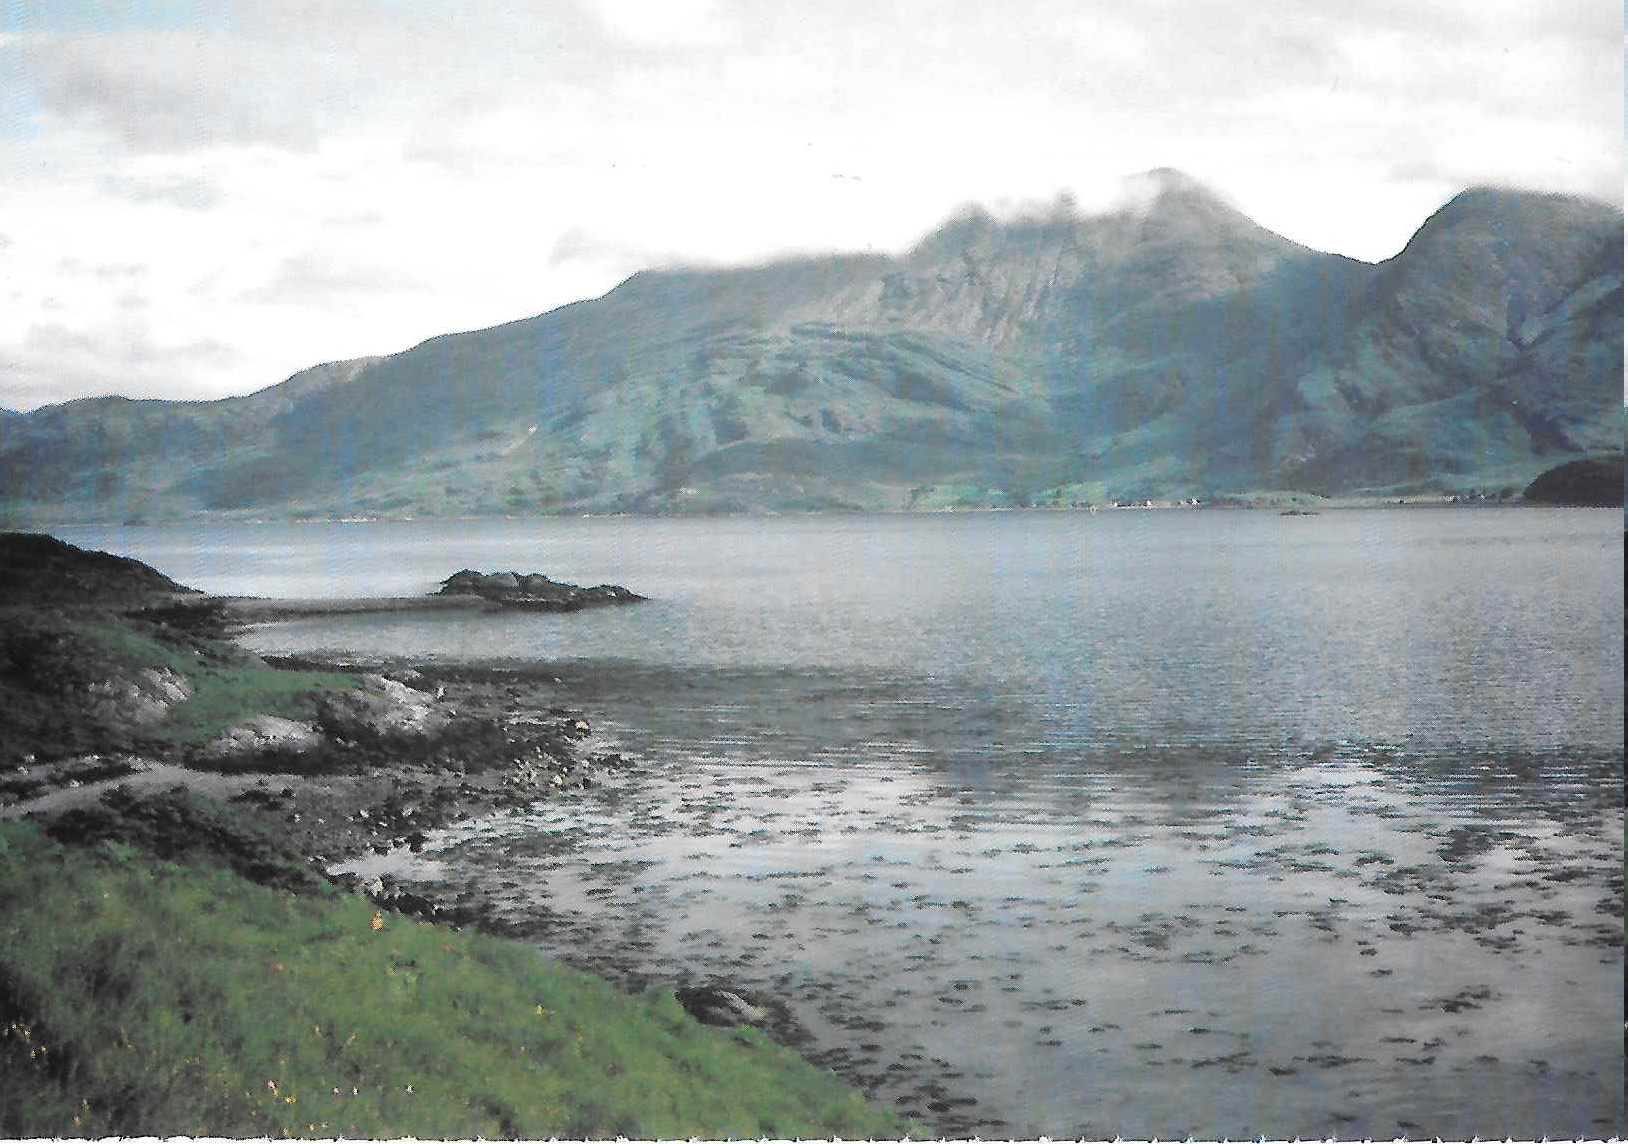
\includegraphics[width=.9\linewidth]{./images/Ben_Sgitheall_from_Loch_Hourn.jpg}
\caption{\label{fig:org5312618}
Ben Sgitheall from Loch Hourn}
\end{figure}

\chapter{Benighted on the Ben}
\label{sec:org7a1677d}
\chapterauthor{Ian Barton}

It was early January when six of us travelled up to
Scotland. Arriving in Glencoe in the small hours, we crept into the
bunkhouse at The Kingshouse and collapsed on the floor intending to
make an early start. Naturally we overslept, but still managed to
leave without paying, creeping past Big Ian who was watching breakfast
TV in his house.

There was the usual chaotic sort out of gear at the golf
course before beginning the slog up to the CIC hut. Inevitably I put
my boot through the frozen crust of peat at the start of the path
which, resulting in a cold wet foot. It had been a cold, clear night
with a fine dawn but a storm was forecast later in the day.  I walked
quickly up the coire and on reaching the hut, I collapsed outside and
waited for Andy to catch up. Fortunately he was even more unfit than
me and I was well rested by the time arrived. As soon as Andy reached
the hut it started to cloud over and flakes of snow began to
fall. After some discussion we decided to go for Glover's Chimney
. Neither of us had done it before and it was a relatively short
route, albeit with the crux at the top which we hoped to climb before
the weather really closed in. We geared up next to the hut on the
pretence that gear you are wearing always weighs less than gear
carried in your ruck sack.

It had been freezing hard for a couple of weeks but there had
been no thaw consequently, the way up into Coire na Ciste was a wallow
in deep powder. This was Andy's first winter route since our trip last
year another epic in Crowberry's Left Fork and he was feeling the
strain. Despite numerous pleas to be allowed to go down on the pretext
that he was totally knackered, I finally cajoled and persuaded him to
the bottom of the route where he promptly collapsed into a mini
bergschrund.

I uncoiled the ropes and stuffed Mars bars into his mouth in
an attempt to revive him. My observation that, although we had not yet
started climbing, we now were almost at the summit and so could not
possibly go back to the hut, was not too well received!

Leaving Andy to sort out the ropes I wallowed over the
bergschrund and managed to get myself established on the first
pitch. The ice was very brittle and I despatched a few dinner plates
down the hill to keep Andy awake. Confident that this first ice fall
was only about a hundred feet long I was puzzled when I ran out of
rope about thirty feet from the top and was forced to belay on a
couple of poor ice screws. By this time Andy had recovered a little
and made short work of seconding this pitch.

The next few hundred feet looked straightforward but devoid of
belays, so I asked Andy to start climbing as soon as the rope went
tight. The weather had closed in and there was a constant stream of
spindrift pouring down on us as we climbed. At the top of the easy
section I went too far left and had to teeter back across a rib of
rock to regain the gully.

Eventually I arrived below the final chimney and began to look
for a belay. After spending some time searching for a peggable crack
without success, I noticed a peg sprouting from the gully wall right
next to me and hurriedly tied on. I had just managed to arrange the
Sticht Plate when Andy arrived.  "That was a very long pitch," he
said.  "Yes," I replied, "about three hundred feet I had to stretch
the ropes a bit! We've only got to get up this little chimney and then
we are at Tower Gap."

The crux chimney proved deceptively awkward, not helped by a
lack of ice where it mattered most. I spoilt the illusion that I was
confident and in control by performing an energetic mantleshelf to get
onto Tower Gap and then falling down the far side. Luckily the rope
drag stopped me after only a few feet.

Andy used his secret weapon, the Alpenstock, to overcome the
crux. Not possessing any axes of his own, the only ones he had been
able to borrow were a couple of very long walking axes.  These
actually proved ideal for the route enabling him to reach right past
the crux and plant them firmly in the good ice at Tower Gap.

"Can't see what all the fuss was about. Why didn't you just
reach up to the good ice on the top?"  It was by now almost dark and
speed was essential. I set off up the rest of Tower Ridge in a hurry,
impressing on Andy the awful consequences of a slip into the unseen
void from the ridge.  However, there were no further technical
difficulties and we reached the top of Tower Ridge just as it got
completely dark.  "It's OK," I said. "I've got all the compass
bearings written down in the front of the guidebook. If we go to the
summit we can go down the tourist track from there."

Setting off on the correct bearing, we counted the paces but
failed to find the summit. Retracing our steps on a back bearing, we
then failed to find the top of Tower Ridge again and so were totally
lost.

"Oh well, never mind, if we just keep going heading west we
should get down to the col eventually."  We felt our way along the
summit plateau but eventually ran into steep ground. Mindful of an
accident to a couple of friends the previous week in similar
conditions, we decided to bivvy.  "Let's just dig a ledge by this
boulder and sit it out till morning."  "What do you mean, you've
forgotten your bivvy bag? Oh well, if I empty my sack into yours you
can use that, it's got a bivvy extension."

Some time later, after everything was sorted out, we settled
down and ate the last remaining chocolate.  "Your rucksack doesn't
meet the bottom of my cag and the spindrift is blowing up my shirt,"
complained Andy.  "It's incredibly boring sitting here."  "I've just
found my hip flask and it's half full of Grouse."  A drunken couple of
hours passed by as the contents of the hip flask were consumed.  "What
time is it?" I asked.  "About seven o'clock."  "Oh good, it will be
light in a few minutes."  "No, it's seven in the evening!"

At this point I threw a wobbler and declared that I was not
going to sit there for another twelve hours freezing to death.  Andy
was also extremely cold and readily agreed to another attempt at
descending. We repacked all the gear and after a short conference,
huddled round the map, decided to set off on a bearing of due south.

Staggering along by the light of the head torch, we remained
roped up in the best tradition, ensuring that we would both die should
one of us slip. After what seemed like hours stumbling downhill we
finally dropped below the cloud to see that we had emerged at one end
of Glen Nevis the wrong end!

Some time later we reached the road and we were not looking
forward to the five mile trudge back to Fort William. However, luck
was with us and two farmers in a Land Rover offered us a lift. They
claimed to have been driving along the glen shining a searchlight up
and down it to try and spot a fox which had been molesting sheep. They
were armed with a rifle to dispatch the animal but it had proved too
cunning and remained hidden. They left us at the Nevis Bank Hotel
where we had arranged to meet the others. Inevitably there was no sign
of them but after we had drunk a couple of pints the barmaid came
over.

"Are you two supposed to be meeting someone here?"  We replied
that we were indeed.  "Oh good, they've left this note for
you."  Unfolding the note we read the following: "If you
aren't dead please can you go to the Police Station and tell
them. We have gone to the Red Squirrel in Glencoe."

Trudging round to the Police Station we informed the policeman
on duty that we were still alive despite appearances to the contrary
and asked for directions to the chip shop.  Failure to get a lift to
Glencoe at midnight forced us to pay for a taxi and we arrived at the
Red Squirrel somewhat dispirited and tired.

The others were pleased to see us and we were made to relate
our story.

"Did you tell them at the Police Station that you were back
safely?"

I replied in the affirmative.

"When we went to report you missing they were really good to
us and made us all cups of tea!"

There's no justice.
\begin{figure}[htb]
\centering
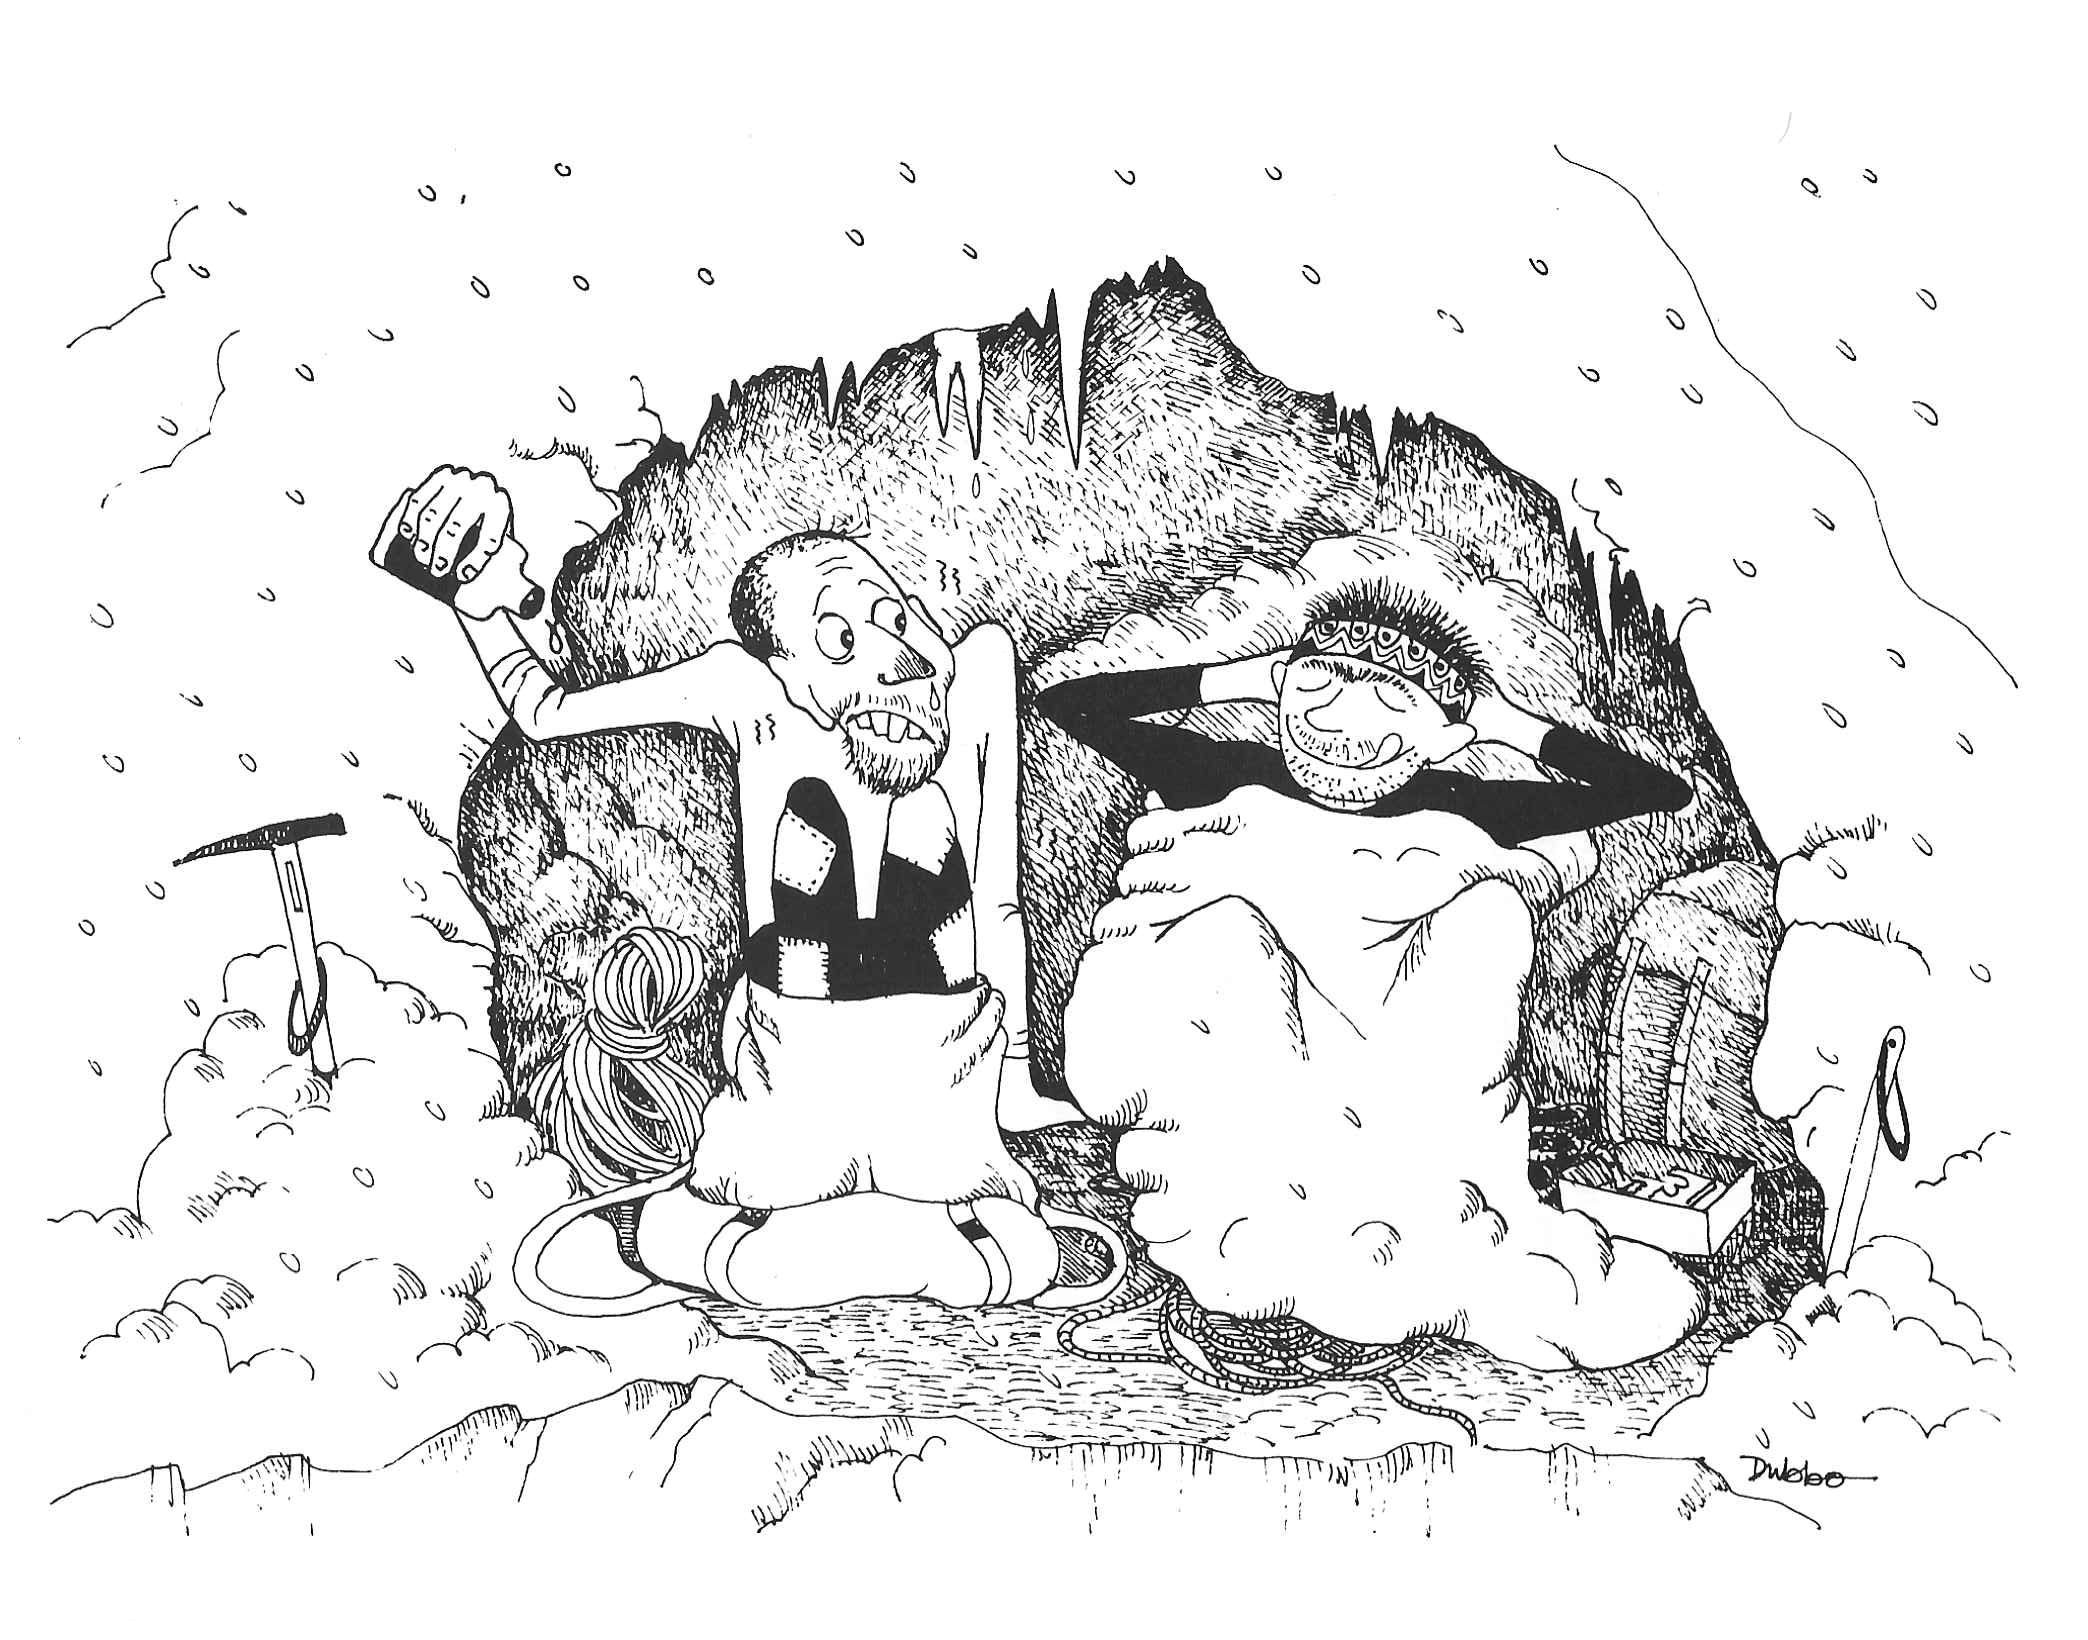
\includegraphics[width=.9\linewidth]{./images/Cartoon_05.jpg}
\caption{\label{fig:orgd909c26}
Benighted on the Ben}
\end{figure}

\chapter{May Day Meet}
\label{sec:orga665025}
\chapterauthor{by Martin Whitaker}

"Esoteric" may well describe some of the rock climbs in the
Central Wales Dolgellau area and the selection that the weather
permitted us to savour over the May Day Bank Holiday ranged from
the sublime   Will o' the Wisp   to the ridiculous   Gorilla's
Armpit     but more of that later.

Frank and Jennifer Mellor went down on Friday morning and
were so amazed to find the sun shining in Wales that they felt
they had to bag  Will o' the Wisp   Hard V Diff   the "Classic
Rock" route  while they could. They had the crag to themselves!
Marian Birkett, Chris Wright and I met them in The Cross Foxes
that evening and Charles Knowles and John turned up soon after.

Saturday morning had us somewhat aghast   sunshine and puffy
white clouds. The setting of the campsite at Cwmrhyddfor in these
conditions seemed idyllic. Ian Lauriston and Steve Hartland
turned up while we were breakfasting, followed shortly by Hilary,
Rosy and Andy. The vote went overwhelmingly for  Will o' the Wisp
with Frank and Jennifer opting for a day on Cader Idris.

Round in Cwm Cywarch there were some tense moments as the
teams battled to be first on  Will o' the Wisp . It seemed that the
Whitaker Birkett Wright team would win, having set off first from
the campsite, but stunning views up the Cywarch valley had caused
a halt at the roadside  for photography and as a result the
Lauriston Hartland team arrived at the parking spot only a short
while after them and raced off towards the crag whilst I was
looking for my boots. However, in the end Ian must have lost his
competitive concentration and I was able to sneak up the first
pitch trailing the ropes while Marian was still putting on her
EBs. As it happened there was no queueing and Chris soloed along
quite happily behind us. With the arrival of Charles, John,
Hilary, Andy and Rosy there was not a single pitch of  Will o' the
Wisp  which was not being climbed on by the CMC at the same time
as the first team arrived back at the sacks, the last one was
just leaving the ground! The route was accomplished without fuss
by all members and we won't mention the top rope that Charles had
on the "rib" pitch. Oops, sorry Charles!

After that Steve and Chris turned to the harder stuff before
being rained off on  Acheron. Marian, Ian and I went off in search
of  Gem   Hard Severe  performing a sheep rescue en route. This
route was made most memorable by the two seconds indulging in a
whimpering contest and comparing notes on every stance about why
they felt they should retire from climbing. The crux pitch
brought the whimpering to a crescendo but nobody actually fell
off, thanks to the "talking upwards" performed by those holding
the ropes above. However, my suggestion that we should follow
this with VS the girdle traverse of Tap Rhygan Ddu was greeted
with a show of apathy that bordered on the brink of flat refusal,
so I abandoned the project. Competition then became quite fierce
as to which one would  not  do another route with me. My suggestion
of a VS had left me with no one to climb with, so I compromised
with a Hard V Diff. Suddenly, they both didn't mind climbing
again, so we raced off up to  Jack of Diamonds .

We arrived at the start just ahead of Andy and Rosy, who had
been climbing  Incapability   Mod  just ahead of Charles, John and
Hilary. It was now looking as if it were about to rain, so Ian
dropped out and Marian and I set off. Halfway up the second pitch
the downpour started and the CMC were soon in full flight,
abseiling from everything in sight. Except, that is, for Marian
and I, somewhat more committed and for whom getting off seemed as
much of a problem as carrying on   so we carried on. As it turned
out, the deluge was only a passing torrent and it stopped soon
after we had reached our sacks.

Back at the campsite, the field had become a sea of mud and
I was rather surprised to find the car's back end overtaking me
as I swung up the hill to the tent. I never did get the car back
up that hill! Our chosen pub was chiefly memorable for its awful
beer   we'll remember not to go there again.

During the night the rain set in and the next morning there
was a marked absence of enthusiasm to leave the pit. As I
expected, the "mountaineers"  Andy, John, Hilary, Rosy and
Charles  set off up Cader Idris leaving the crag rats and Frank
and Jennifer to elect for "a day at the seaside". We rendezvoused
in Towyn at lunch time, a good enough excuse for a visit to the
chippie   rather interesting pasties and bright green peas! For
the afternoon's entertainment we relied on Marian's age and
experience: from the depths of ancient history, almost before
time began, she remembered going on a rock climbing course when
she'd been taken  to a small training crag on a beach, somewhere
near Towyn. So we set off for crag X and with remarkable speed
and accuracy, were soon at the foot of a small but fine little
sea cliff with clean solid rock  albeit a little wet  and lots of
excellent little lines and problems. There was even a climbing
course of young lads and lasses in residence to provide further
entertainment. Soon everyone was engrossed in leading, seconding,
top roping or soloing, enjoying themselves so much that the
weather gave up in disgust and the rock dried out.  By about five
o'clock most of the obvious lines  and some of the climbers  were
exhausted.

Steve and Ian headed back to Sheffield, but the rest decided
to sneak a route on Bird Rock whilst the weather wasn't looking.
Frank and Jennifer climbed  The Buttress   V Diff  and Marian and I
went for an amazingly steep route called  The Jug   Severe . Whilst
this was in progress the mountaineers turned up, having had a
good day on Cader. The pub at Abergynolwyn was a great success
more friends of Marian's arrived to swell the numbers and a good
long evening's boozing was enjoyed by all.

It rained most of Sunday night but had the decency to stop
when it was time to get up, breakfast and pack. The mountaineers
went off to sample Marian's sea cliffs, Frank and Jennifer went
for a bike ride and we headed for Bird Rock again. This crag has
a propensity for excessive steepness   disconcerting until you
discover that it has a fair number of large, juggy holds on it.
Unfortunately, a high percentage of these seem to be inadequately
secured to the rock face and one at least is secured no longer,
having parted company when I was clutching it, with the
inevitable effect of causing me to execute a swift flight through
space before a friendly Moac helped me to resist gravity's
summons. Unfortunately, my other hand had been stuffed up a
particularly sharp crack when I was betrayed by this hold and as
a result I finished the route using blood for aid  it gives
better adhesion than chalk!  I fell off the most  solid  pitch of
an HVS called  Gorilla's Armpit   even the name is enough to put
you off!   Ollie's pitch was a real frightener, swinging across
on massive, apparently unsupported, blocks. I was glad to make it
the last route of the holiday.

Meanwhile Chris and Dave attacked  The Bolero   HVS   and
Spike Wally   VS  and Lisa, Pippa and Marian formed a Cordee
Feminine for  The Diagonal   Severe  and  Siesta   Severe . A good
time was had by all and by all accounts we had better weather in
Wales than was to be had in the Peak   can you believe that?

\begin{figure}[htb]
\centering
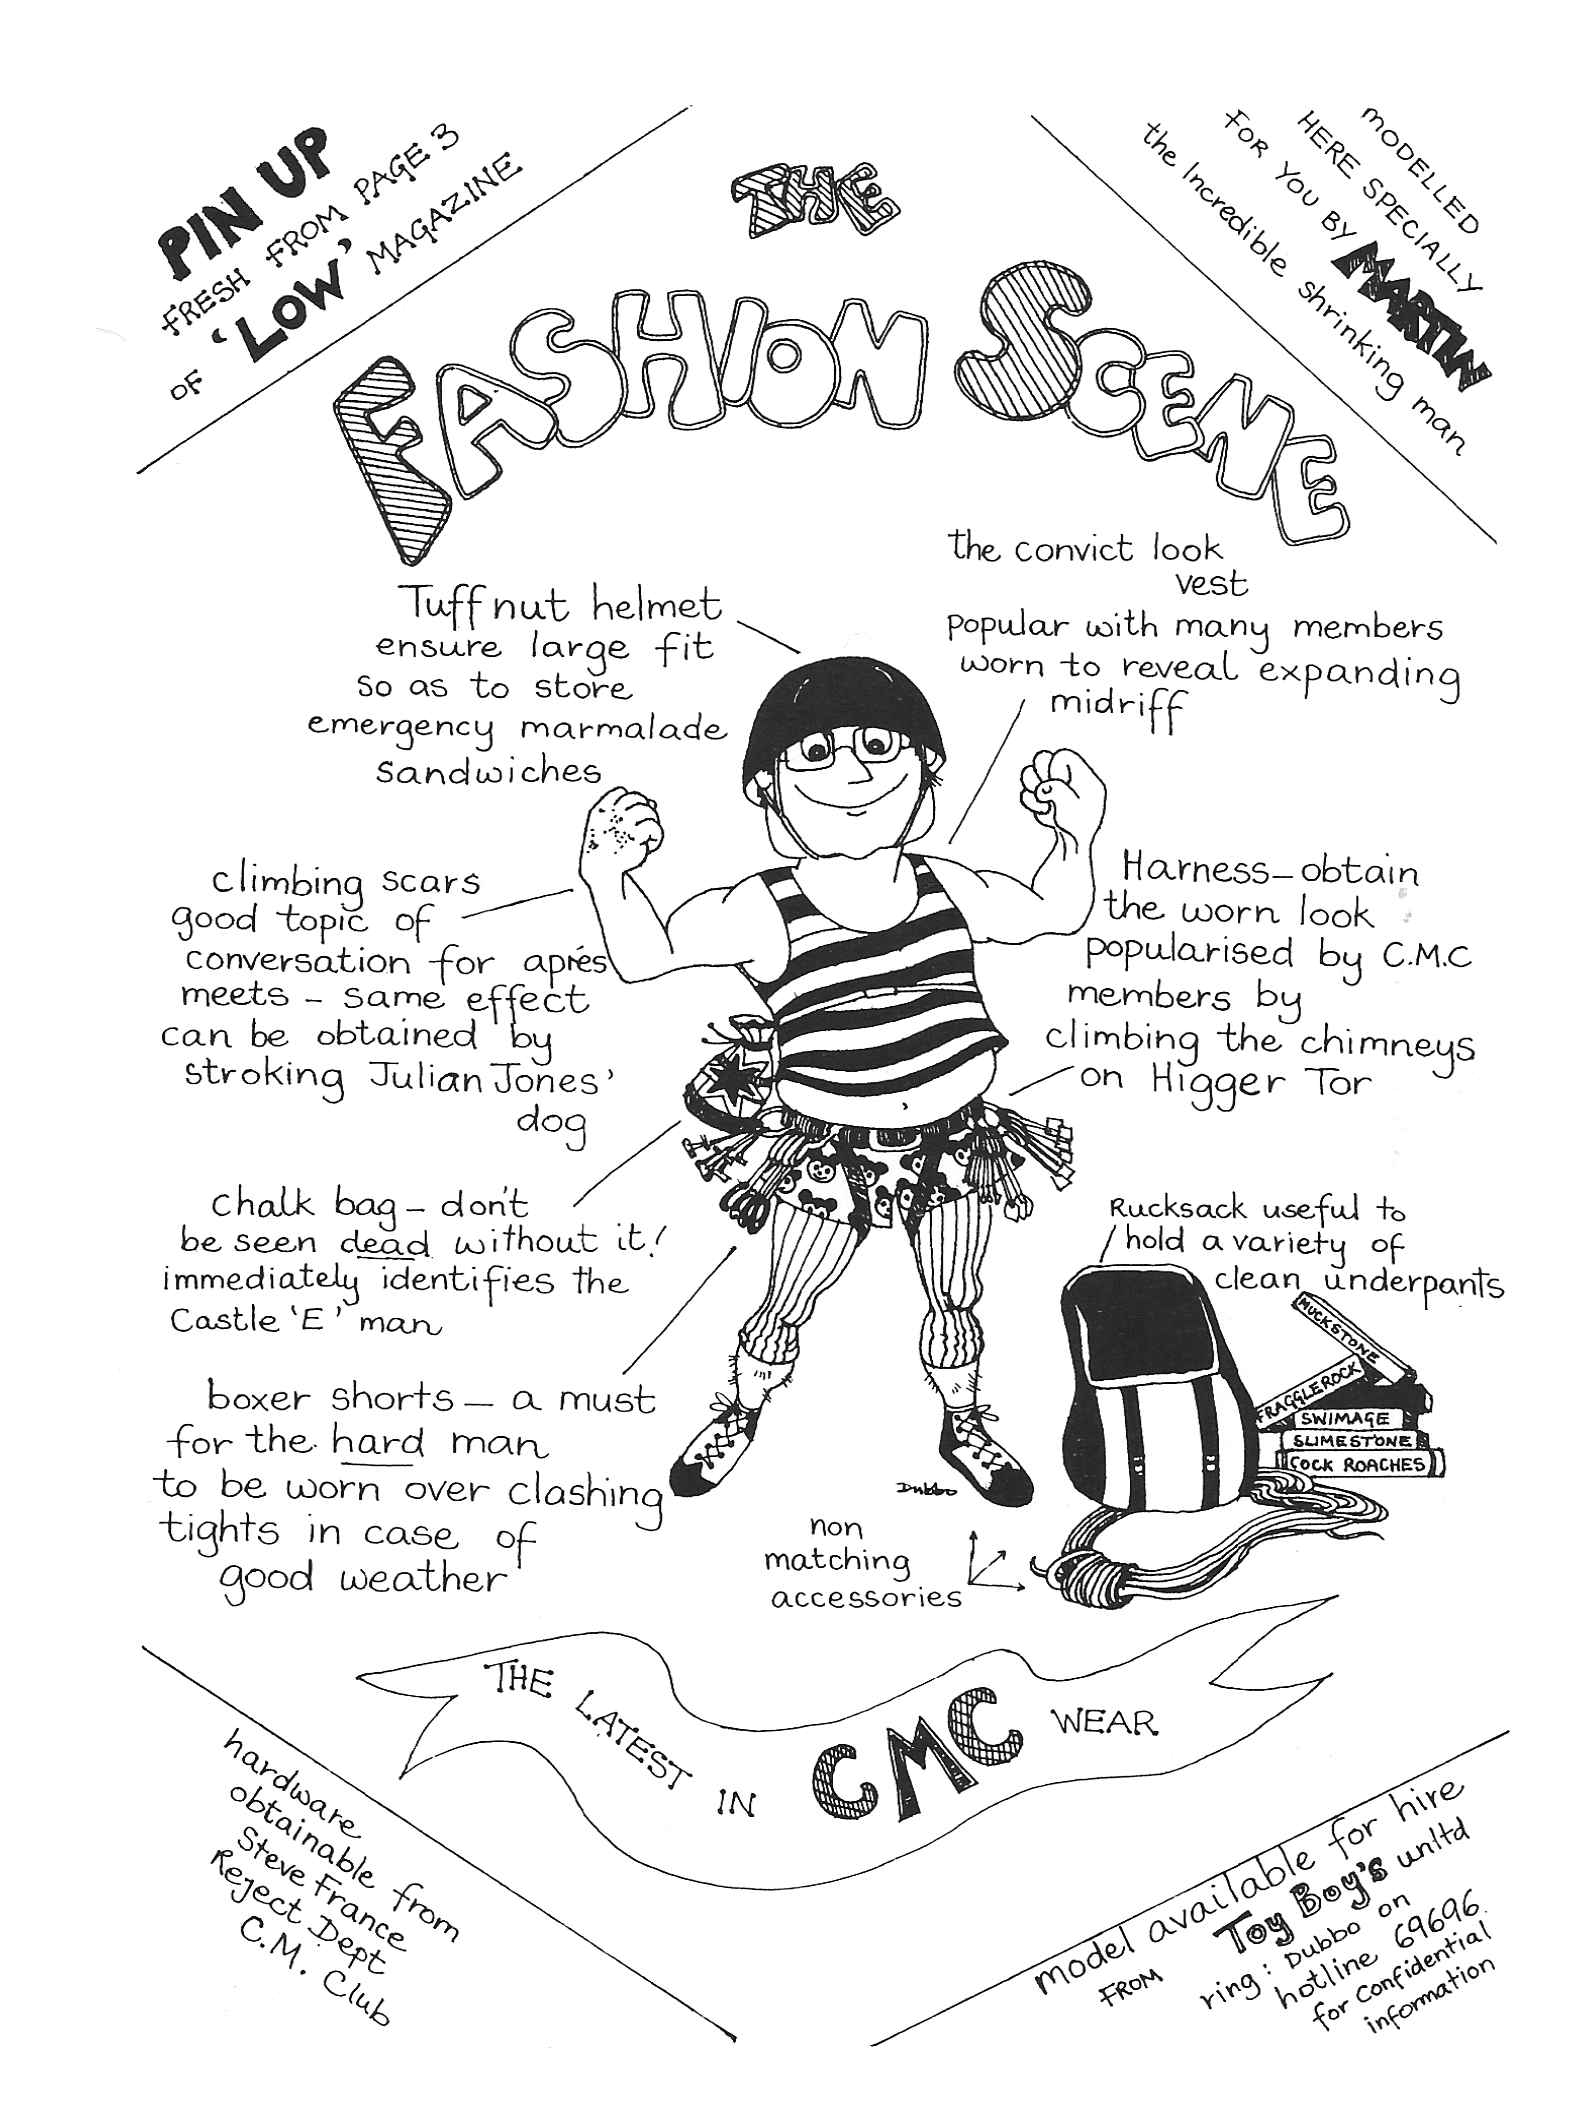
\includegraphics[width=.9\linewidth]{./images/Cartoon_06.jpg}
\caption{\label{fig:orga710269}
May Day Meet}
\end{figure}

\begin{figure}[htb]
\centering
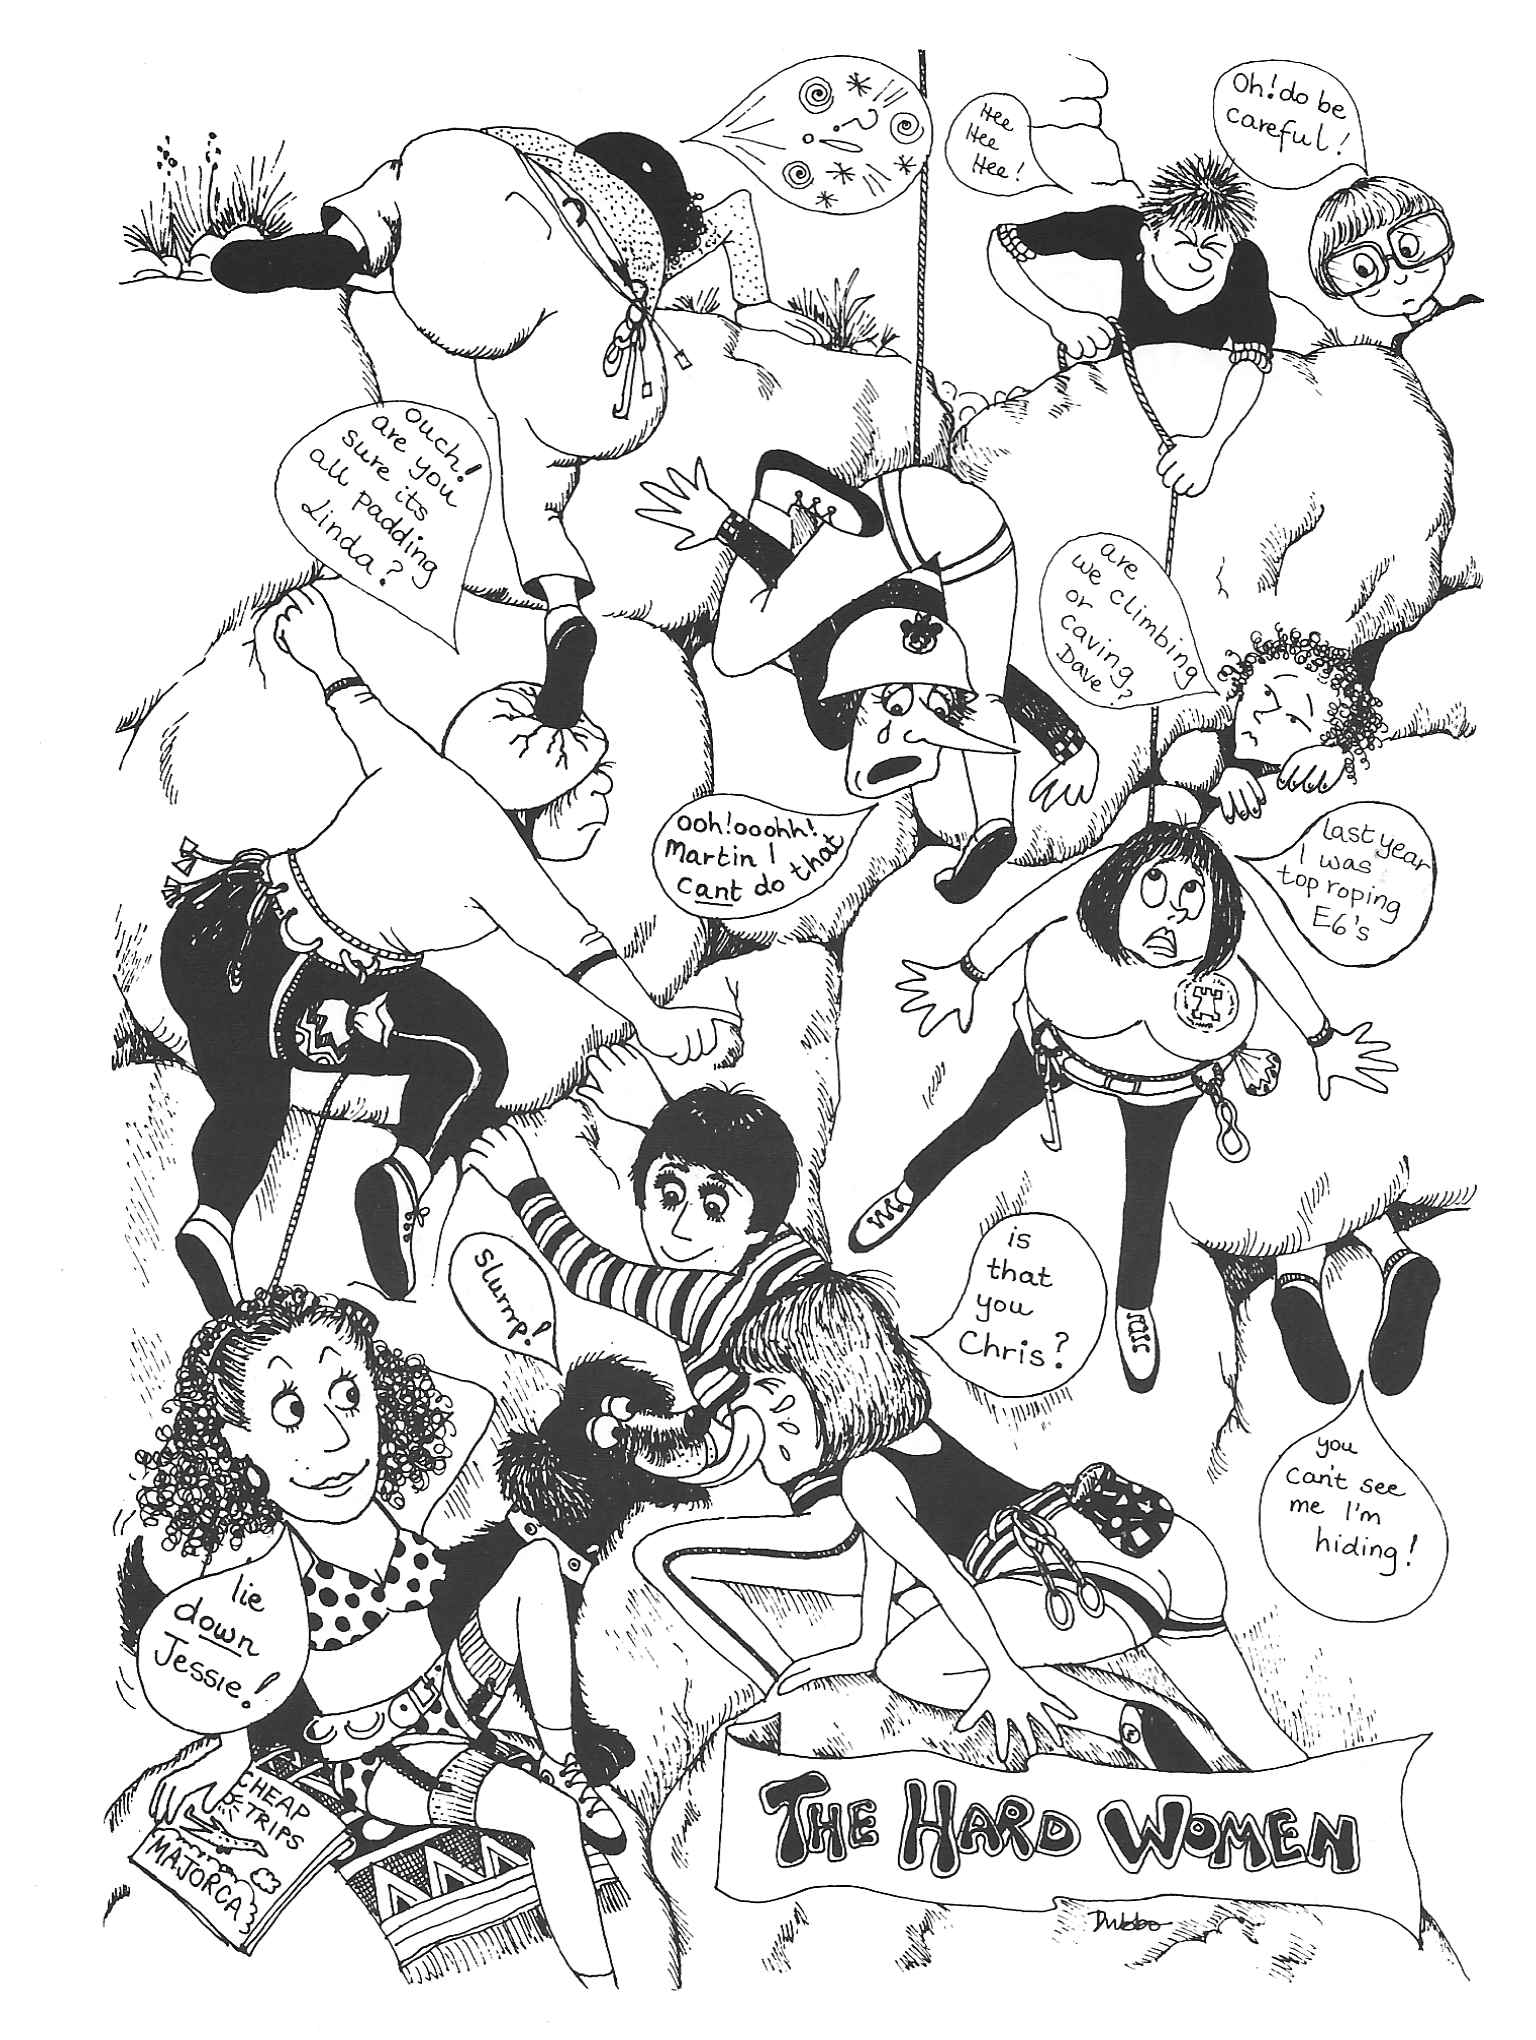
\includegraphics[width=.9\linewidth]{./images/Cartoon_07.jpg}
\caption{\label{fig:orgf4acfcd}
The Hard Women}
\end{figure}

\begin{figure}[htb]
\centering
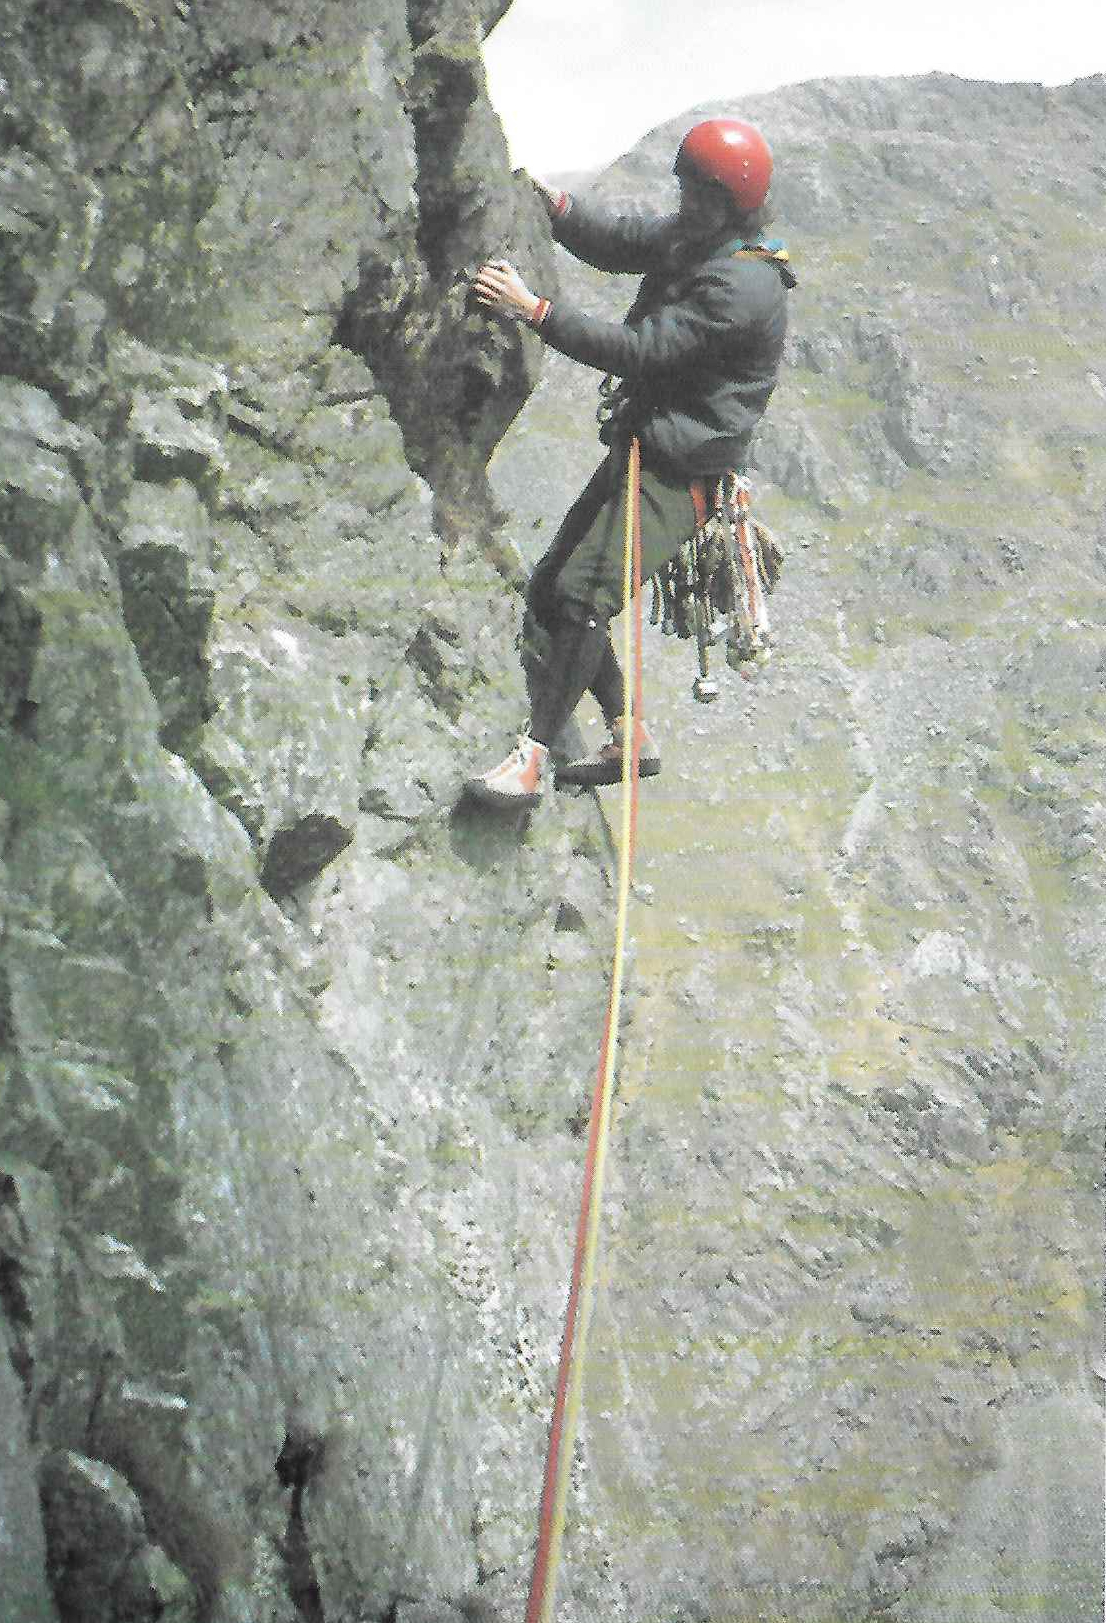
\includegraphics[width=.9\linewidth]{./images/Julian_Jones_on_Acheron_Cwm_Cywarch.jpg}
\caption{\label{fig:org3be7224}
Julian Jones on Acheron Cwm Cywarch}
\end{figure}

\begin{figure}[htb]
\centering
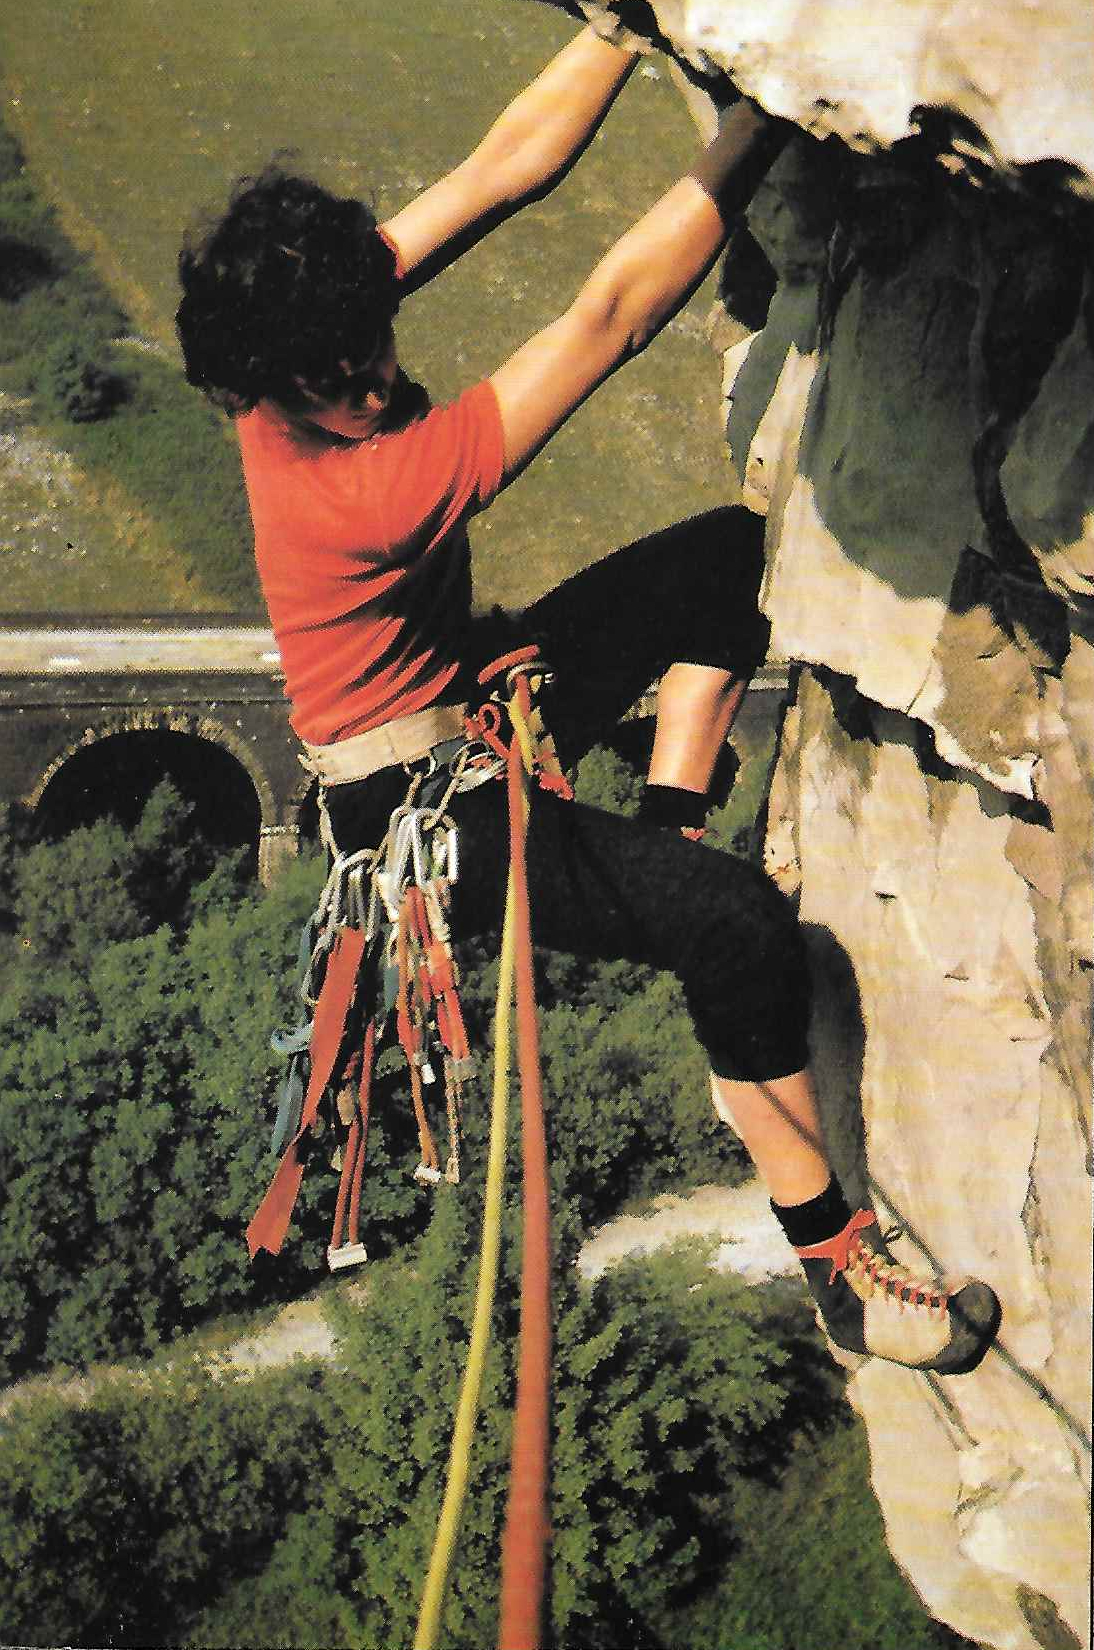
\includegraphics[width=.9\linewidth]{./images/Steve_Hartland_on_Sirplum_Cheedale.jpg}
\caption{\label{fig:orgc415be1}
Steve Hartland on Sirplum Cheedale}
\end{figure}

\begin{figure}[htb]
\centering
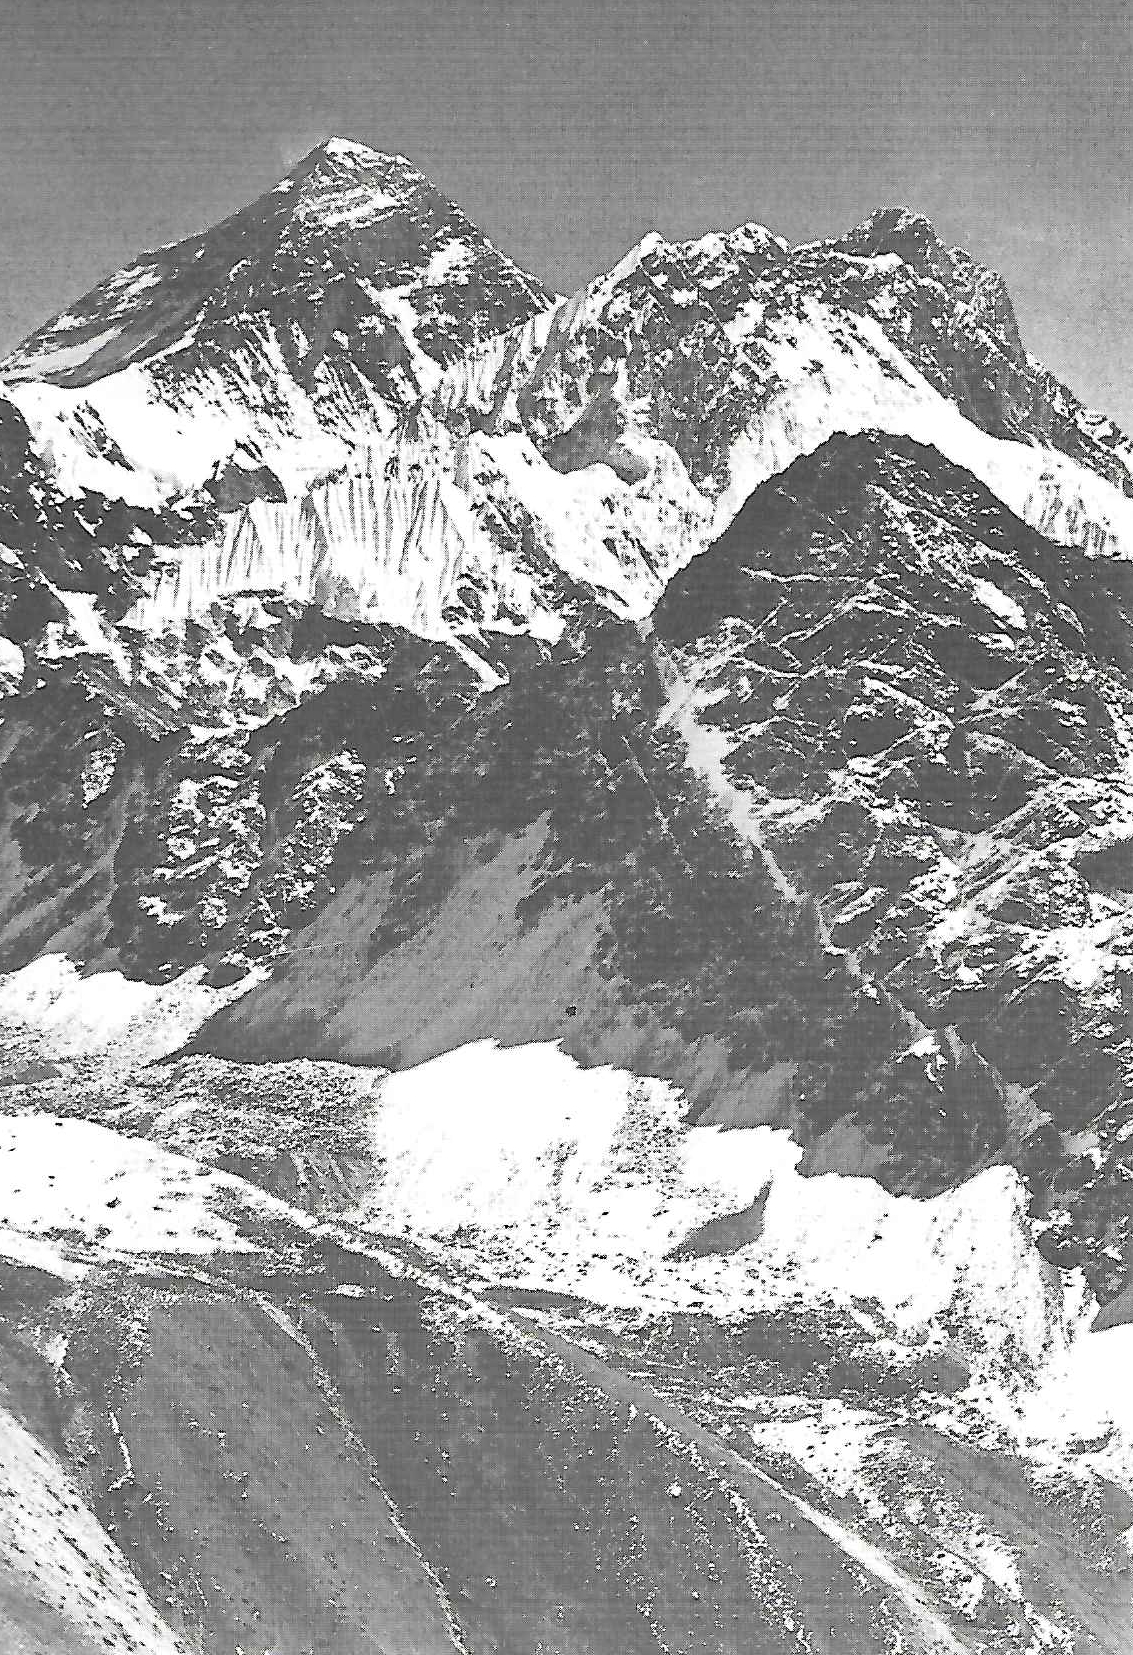
\includegraphics[width=.9\linewidth]{./images/Everest.jpg}
\caption{\label{fig:org0359462}
Everest}
\end{figure}

\chapter{A Trek in the Andes}
\label{sec:org6743fc9}
\chapterauthor{Bob Madeley}

The Cordillera Blanca in the Peruvian Andes is one of the
most beautiful mountain ranges in the world, with peaks reaching
a height of more than 6000m. Although not as high as the great
giants of the Himalaya, these mountains hold second place to none
in shape and grandeur. It was with the prospect of experiencing
this grandeur that eleven of us, led by Alf Gregory  Greg , set
off from England with perhaps a little trepidation to this wild
area on the other side of the world.

After two days in the bustling city of Lima we left by bus
on the 250 mile journey to Huaraz, crossing part of the Atacama
desert through which passes the Pan American Highway. This is a
road cut through the sand and which in places reaches a height of
one hundred metres immediately above the sea. As we moved inland,
many roads had washed away by floods and rivers and the driver
was often forced to drive along dry, rocky, river beds until the
road could be regained.

After a very hot and dusty ten hour drive punctuated by
several breakdowns, the bus, with very suspect brakes, at last
reached Huarez. En route we had taken a short side trip to the
Parachota Valley on the edge of the High Cordillera. In this
remote valley of sparse vegetation and deep clear "coral like"
pools, we saw the Puya Raimondi which has the tallest flower
spike in the world, attaining a height of eight metres or more.
This plant is confined to the Peruvian and Bolivian Andes and may
live for one hundred years, flowering just once before it dies.
An estimated eight hundred flowers grow on one stalk, attracting
the humming birds which play a large part in their pollination.

A tortuous alpine style road led us above Caraz and the
first sight of a beautifully shaped peak of Santa Cruz got our
adrenalin flowing. The arrieros packed our gear onto thirty five
burros and along with a horse and three scraggy dogs we ascended
the steep gorge which, after three days travel, led us to the
Punta Union Pass  4,750m .

Continental drift, resisted by the Earth's crust below the
Pacific Ocean, has created intense compression and has crumbled
the land's surface, releasing the igneous rocks which form most
of the highest peaks. The effects of glaciation, volcanic action
and water erosion have completed the process and have helped to
form the sheer mountain sides above the deep gorges through which
we passed. The extreme temperatures between day and night, so
near to the equator, continually freeze and thaw the snow and
ice, forming beautiful jagged peaks with grotesque shapes along
the ridges.

Swamp areas, created by the lakes gradually drying out,
seriously impeded our progress yet revealed a vast variety of
beautiful plants and flowers, at their best in June, as we
splashed our way through the clinging bog.

The first stage to the campsite was undertaken on horseback.
Progress was not very fast and yours truly decided to press
ahead, but as the altitude took its toll the raison d'etre of the
horse became obvious. A slap on the rear from the arrieros
persuaded the horse to leap across the river whilst the arrieros
preferred to cross the bridge upstream. The horse was unable to
make the jump and so stopped  I didn't   and scrambled from the
river in a sodden state. From then on, there was a complete
respect by the entire party for the effects of altitude!

Camping in the Cordillera was very comfortable with the
temperature rarely falling below minus five degrees centigrade
and very pleasant evenings were spent around the campfire. The
mess tent was the scene of a pleasant "happy hour" before dinner
when we drank Pisco   a grape brandy to which we took quite a
liking   followed by an excellent meal prepared by the arrieros.
As darkness fell lights appeared from other campfires high on the
hillside where itinerant Indians were spending the night.
However, we slept well as our dogs were very capable of keeping
any light fingered intruders at bay.

Early morning: dawn was greeted with tea brought to our
tents at 6.30 am. An excellent breakfast was taken as the sun
rose and we were off again. The climb to the Punta Union was very
steep as we wound upwards along the zig zag, rock strewn path. We
passed by the very edge of glaciers below the four peaked summit
of Taulliraju  5,830m , which dominated the scene with its jagged
serrated ridges, lit up in the early sunlight.

A long time was spent on the summit of this pass, partly for
a desperately needed breather but mainly to take in the wonderful
panorama. Everywhere was silent, the snow white and glistening.
The Pass is guarded by Taulliraju, its vast glaciers tumbling
down into a deep turquoise lake far below, whilst overhead we
caught our first glimpse of a Condor soaring above the ridges.
The sun became hotter, there were deep rumblings and an avalanche
fell down the mountainside   then all was silent once more.

Once over the Pass we descended across bog land through the
Huaripampa when we returned to lush vegetation and beautiful
flowers. On the way we passed several medium sized Indian
villages where we were made very welcome. Village land is
generally owned collectively and the rural Indians live virtually
outside the money economy. Day to day life is organized on the
basis of mutual help  big jobs, such as harvesting, threshing and
house building are done with the help of neighbours, who in
return receive help when needed. In spite of their apparent
poverty, we certainly had the impression that they were a happy
and contented people. A wedding was taking place in a nearby
village and the procession passed us by on the trail, the bride
to be on horseback, the family carrying everything needed for the
festival, and grandma bringing up the rear carrying her kettle.

Along the seventy five mile length of the Cordillera rise
some twenty peaks of over 6,000m, including Peru's highest
mountain, Huascaran, with the world's largest concentration of
glaciers within the tropical zone. Our journey continued over
several high passes and we saw many fine waterfalls which tumble
over cliffs creating delightful patterns in the afternoon sun.

A very stiff climb to the Portachuelo de Rataquena and
suddenly the summit of the Pass was upon us revealing a mighty
panorama of the high peaks of Rataquena, Tocllaraju and Copa,
reaching down into the Honda Valley which was to lead us to our
destination. And then a very rare experience   just below the
summit and on very slippery ice coated cliffs we saw the Rima Rima,
a plant found only in this part of Peru. With its delicate
red flower and large leaves, it seemed more suited to a
greenhouse than to the top of a 5,000m pass. The Indians have a
special reverence for the flower, perhaps because of its success
in surviving in its hostile environment, and some wear it in
their hatbands for good fortune.

On the final descent to Rinoconda the burros seemed to sense
that their labours were at an end and proceeded with renewed
energy over limestone rock, serrated over the years by water
erosion. The river swells in winter and then recedes during the
summer to reveal the strata of the rock and strange formations.
It tumbled noisily through yet another cataract as we reached the
end of our journey to be were greeted by beer, sandwiches and
fruit before loading our equipment back onto the bus.

As we left the high hills for the last time, we looked back
at the beautiful peak of Rataquena with its summit glistening in
the sunlight and reflected on the scenery we had been privileged
to trek through, also the hospitality we had experienced from
everyone we met.

\chapter{Eastern Edges Walk}
\label{sec:orgabeefcb}
\chapterauthor{Frank Mellor}

The main body of walkers assembled at The Flouch Inn at half
past eight on a dry but overcast Sunday morning. An advance party
consisting of the youngsters and parents had left earlier to
allow shorter legs a little more time to negotiate the initial
boggy sections.

The main party was soon heading up Cut Gate, though Jack had
to be restrained from ploughing over the eroded portion of the
path which was fenced off for restoration purposes. Once the
little notice had been read to him and the possibility of wardens
lurking in the conifers had been pointed out, he agreed to the
recommended variation, though not without mutterings about his
preference for going straight up.

The path was followed without further incident until Margery
Hill was attained. Jack now made amends for his previous
indiscretion by imparting a most valuable piece of information
namely that we were now standing on the highest ground in
Sheffield. Fortified by this gem and spiritually uplifted by the
generous manner in which it was given, we felt able to continue
to Featherbed Moss. In a state of euphoria, we wandered
southwards until Abbey Brook lay below us. It was unfortunate
that, as we dithered on the brink, we were witnessed by the
advance party who had taken the more conventional contouring path
around the head of the clough. Now was an opportunity for
individual variation and a dozen people took nearly the same
number of different routes for Back Tor. Everyone arrived within
minutes of each other and a welcome break was taken by all
nineteen walkers, together now for the first time. It was
generally agreed that the most tiring part of the walk was over
and, barring nuclear attack, success was assured. In fact all
that remained was to sit back and we would soon be at The Robin
Hood near Baslow.

As time went by it became evident that a little stroll was
still necessary in order to achieve our objective and so we set
off down Derwent Edge. The view became increasingly more
interesting as we passed Wheel Stones and continued across
Highshaw Clough down to Moscar House.

A short walk up the road, then we were striding away  from
the exhaust fumes toward Stanage. We took another break  near
High Neb since this was reckoned to be the half way point. Whilst
lunching we greeted a passing couple. The young lady returned our
 salutations, but her companion was heard to say "It's The
Castle!" whereupon she was shepherded away along the Edge with
only an occasional backward glance. Shortly after this we met
Dave and Jenny, who had walked up from The Robin Hood where they
had kindly deposited a car for our return.

From Stanage we chose to walk down the Green Drive below
Burbage, rather than over Higger Tor, and thence into Longshaw
where we took a welcome tea break at the cafe. This proved very
refreshing and gave us a lift for the last leg. We were soon over
Froggatt in the gathering gloom, but there was a little stumbling
and grumbling as it got darker on Curbar Edge. Most people had
torches at the ready for the traverse of Baslow Edge and we found
the Wellington Monument without much trouble. Jack attempted to
rid himself of some Grappa at this stage but with little success
  judging by the response of those who were tempted, he will be
offering his bottle round for several years to come!

It was drizzling now so we went at a fair pace down the
track to the crossroads and then made a rather rough crossing up
to Birchen Edge. The path there was a welcome sight and it was
followed easily down to The Robin Hood   which was shut! We had
taken ten hours for the walk, arriving a good half hour before
opening time. A vote of thanks was offered to Jack as we waited,
shivering in the freezing cold evening with only one hip flask of
Grouse between nineteen.
\begin{figure}[htb]
\centering
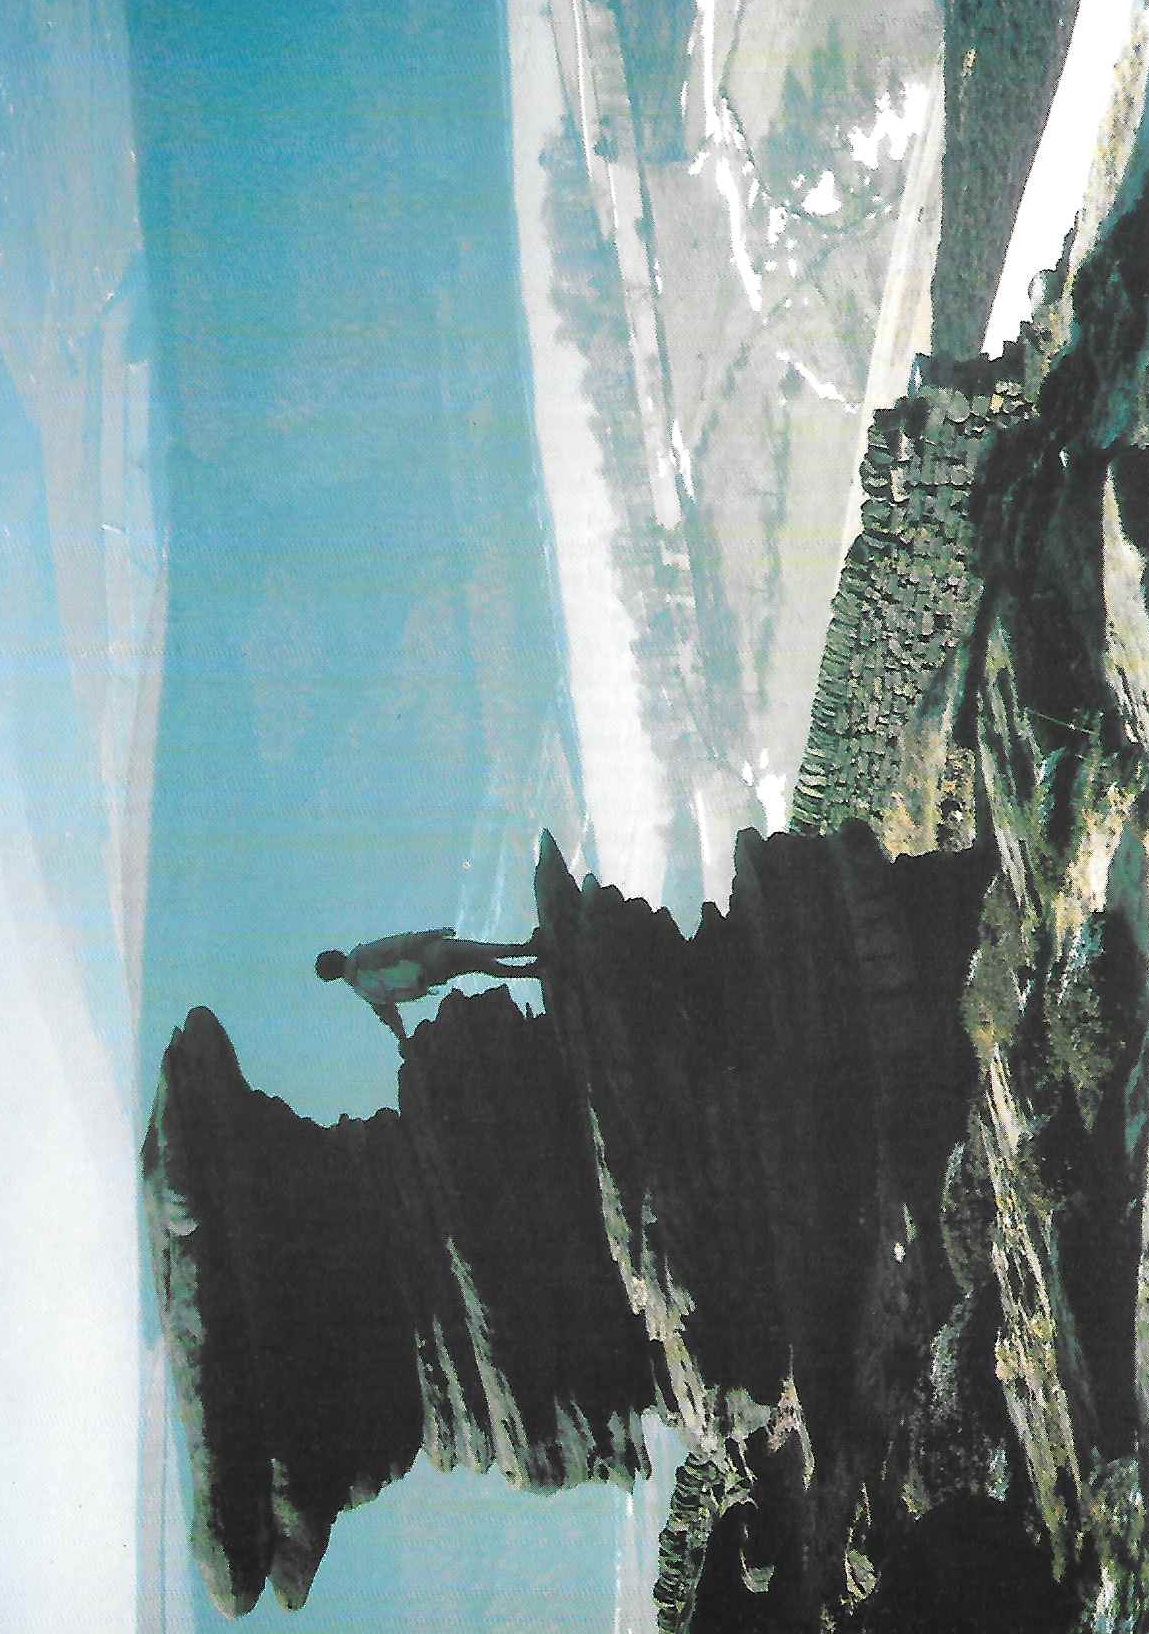
\includegraphics[width=.9\linewidth]{./images/The_Salt_Cellar_Derwent_Edge.jpg}
\caption{\label{fig:org14337f6}
The Salt Cellar Derwent Edge}
\end{figure}

\chapter{Falling Off}
\label{sec:orgf9fb0ff}
\chapterauthor{Mike Doyle}

Climbing is all about getting up. The trick is to ascend
vertically to the top with appropriate downward glances to check
the placement of the feet on foot holds, but without downward
movement of the rapid uncontrolled variety. Deviation from ascent
is permissible by traversing sideways, climbing down or
 abseiling, but certainly not by taking to the air and relying on
gravity.

The reasons for this are, of course, obvious. Firstly,
climbers are land creatures who do not possess wings, so any
attempts at aerobatics will inevitably result in a bumpy landing.
Secondly, the whole ethos of the sport of climbing is to get up.
To fall off is to repudiate this basic principle.

Nevertheless, the art of falling off is sometimes practised
by those who find themselves too stretched to continue upwards.
As with all good mountaineering clubs, The Castle is rife with
stories of those who have fallen off, ranging from the ones who
have got away with amazing scrapes and near misses to those who
have suffered more serious injuries. At various times battered
helmets and frayed ropes have been displayed in the clubroom,
whilst the fallen have themselves limped in on crutches, their
damaged limbs suitably encased in plaster.

The better practitioners of the art of falling off manage to
ensure, by the prior placement of adequate runners and a good
choice of second, the avoidance of contact either with rocks on
the face or the ground at the bottom, so that the fall is no more
than a mere dangle from the last runner. The less able
practitioners of the art fail to keep one or more of these points
in mind and so fail to achieve such an innocuous end result.

Some go quietly, others with much noise and commotion.
Witness the Club member who destroyed the Lakeland solitude on
Dow Crag by noisily dislocating his shoulder, the din of his
painful fall being equalled only by his protests at the rough and
ready on the spot reduction of the injury by a fellow Club
member. Some are not even content with a single incident but
insist on trying again: one notorious case insisted on returning
to the crags with his newly acquired pot only to chalk up another
fall to his portfolio and more Plaster of Paris to his person.

At this stage I have to declare my personal interest in the
matter and admit to belonging to the ranks of the fallen. My fall
was accomplished without noise or loud proclamation and I did at
least achieve dangle   only in my case the dangle was merely
momentary due to the runner not proving sufficient.

It all began innocently enough one sunny May afternoon.
First my left hand slipped off the rock followed by my right hand
and then by both feet. The books tell us that three points of
contact is the rule. And with no point of contact at all further
upwards progress becomes impossible. The result was the forbidden
condition of downward flight. As I saw terra firma approaching at
alarming speed with a painful impact seeming inevitable, my
reaction changed from mild surprise at my sudden airborne status
to abject terror. Contrary to folklore, my previous life did not
flash before me and events did not happen in slow motion. On the
contrary, I made contact with the ground at speed and the result
was both quick and painful. My landing was possibly the most
unskilful aspect of of all, following very much the traditional
warning of the result of a bad landing given to raw recruits in
the Paras: "Toes, knees, hospital!"

Well, there it is, my personal summary of the whys and
wherefores of falling off and how it has worked for me. It is an
activity which continues from year to year and is one which is
inseparable from climbing itself. Without the risk of falling off
there would be no being gripped, no adrenalin and no beer embellished
accounts of scrapes and near misses. Most of the
fallen do resume their climbing careers  some  as I have already
mentioned  even repeat the experience. Personally though, I have
succumbed completely to the downward urge and now practice the
art of caving.
\begin{figure}[htb]
\centering
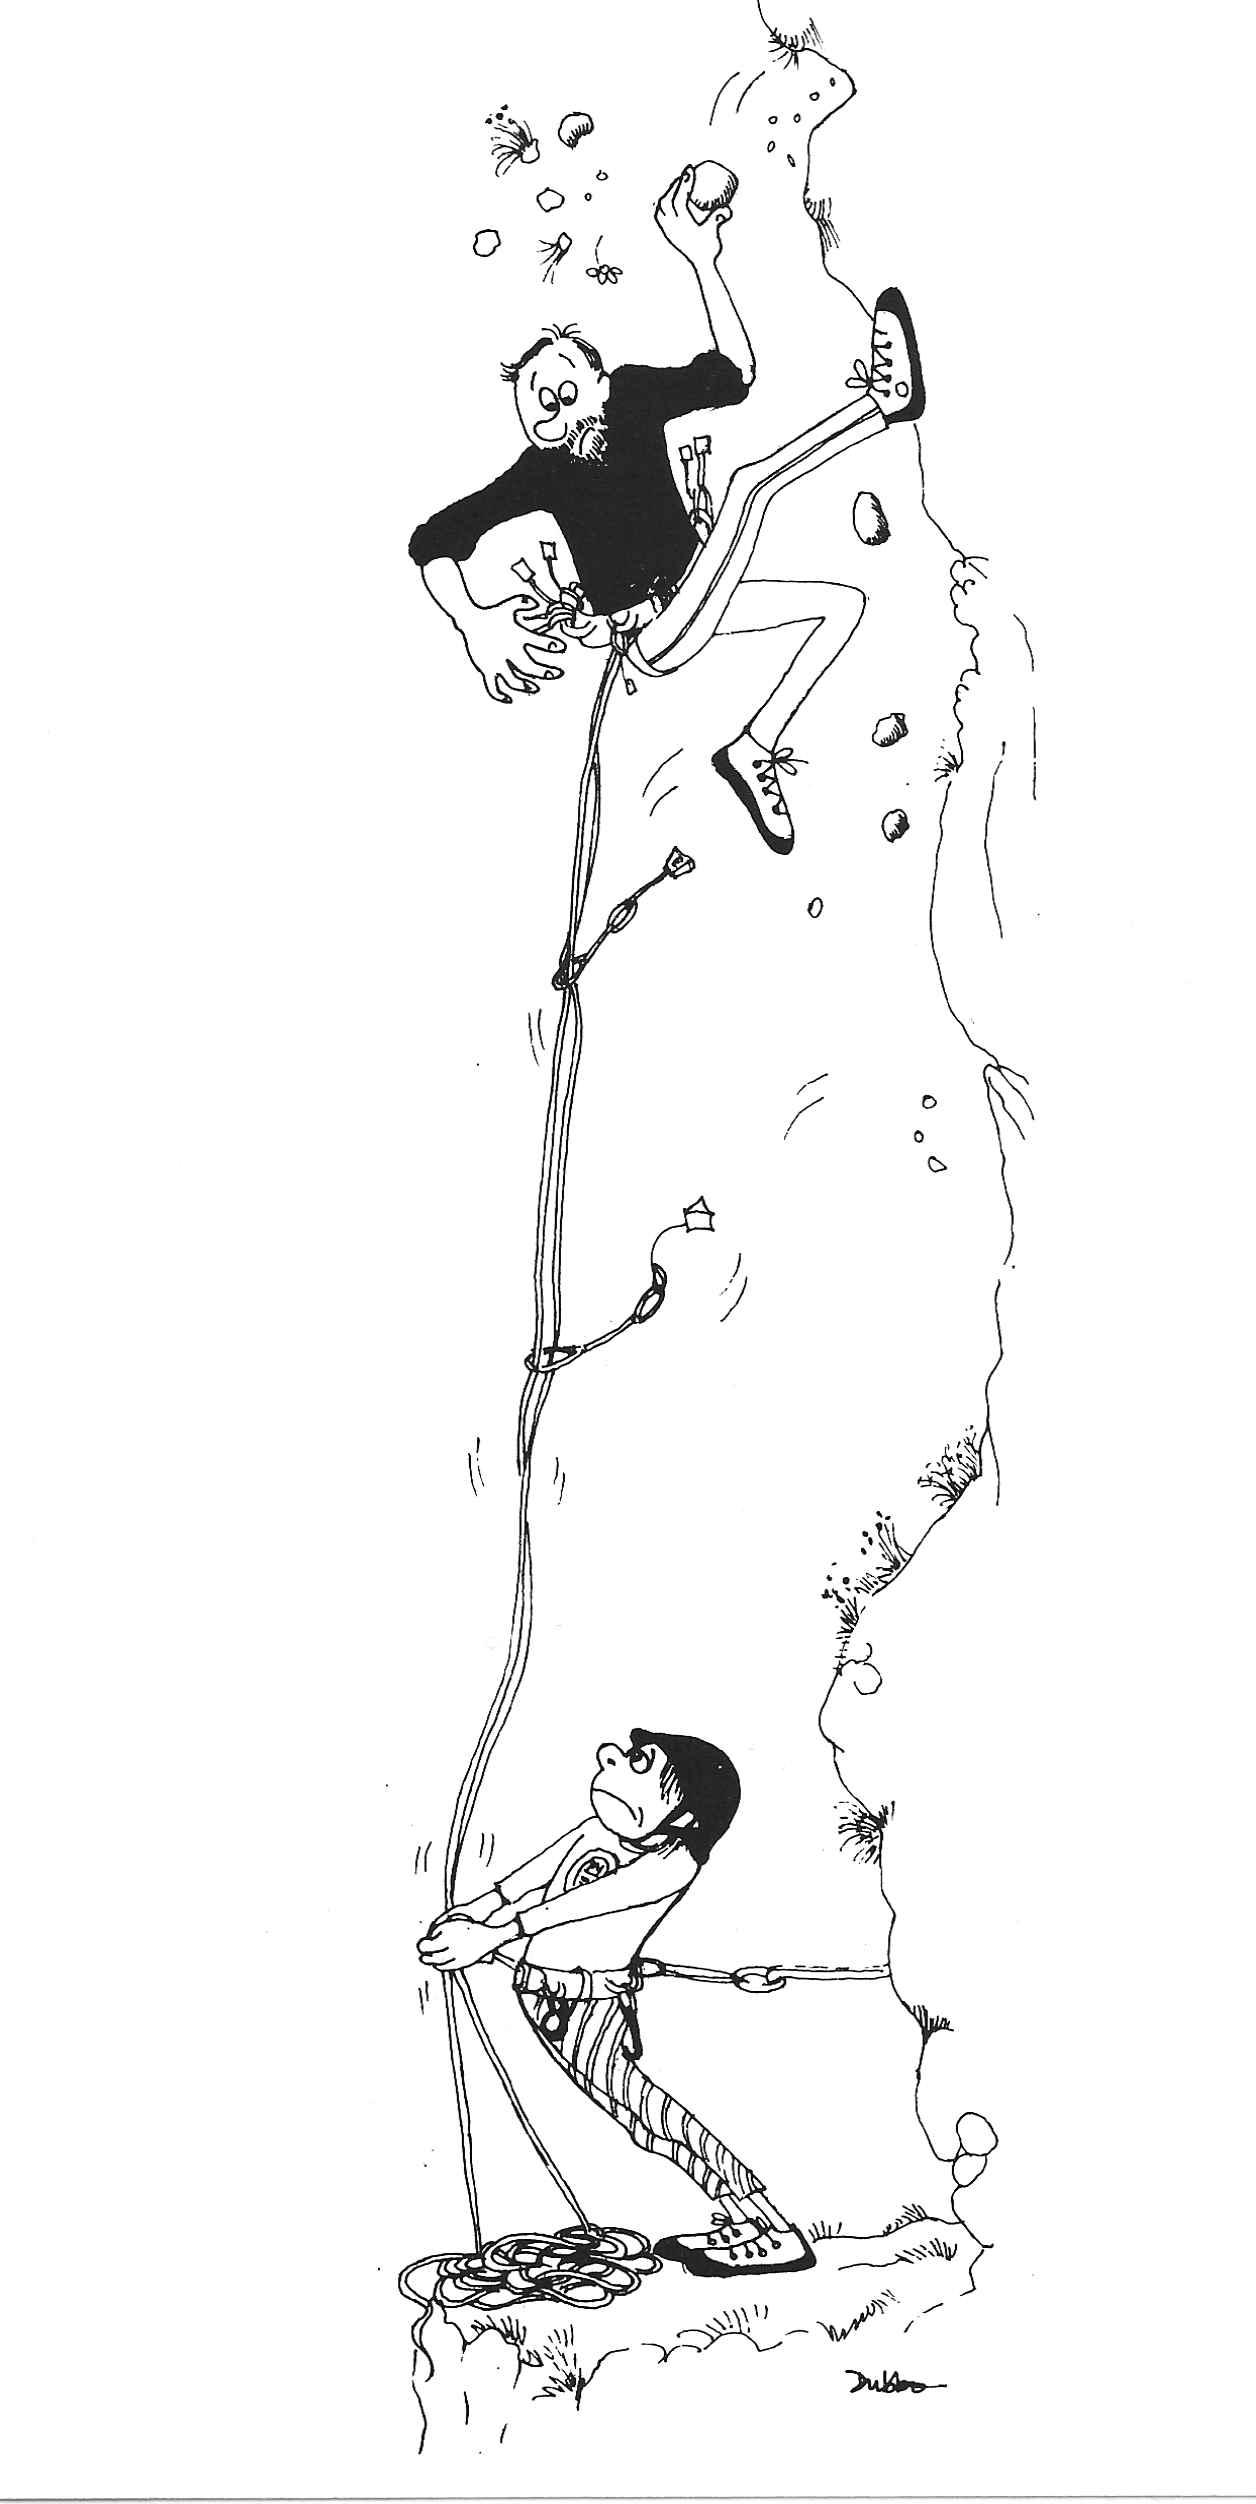
\includegraphics[width=.9\linewidth]{./images/Cartoon_08.jpg}
\caption{\label{fig:org494040a}
Falling Off}
\end{figure}

\begin{figure}[htb]
\centering
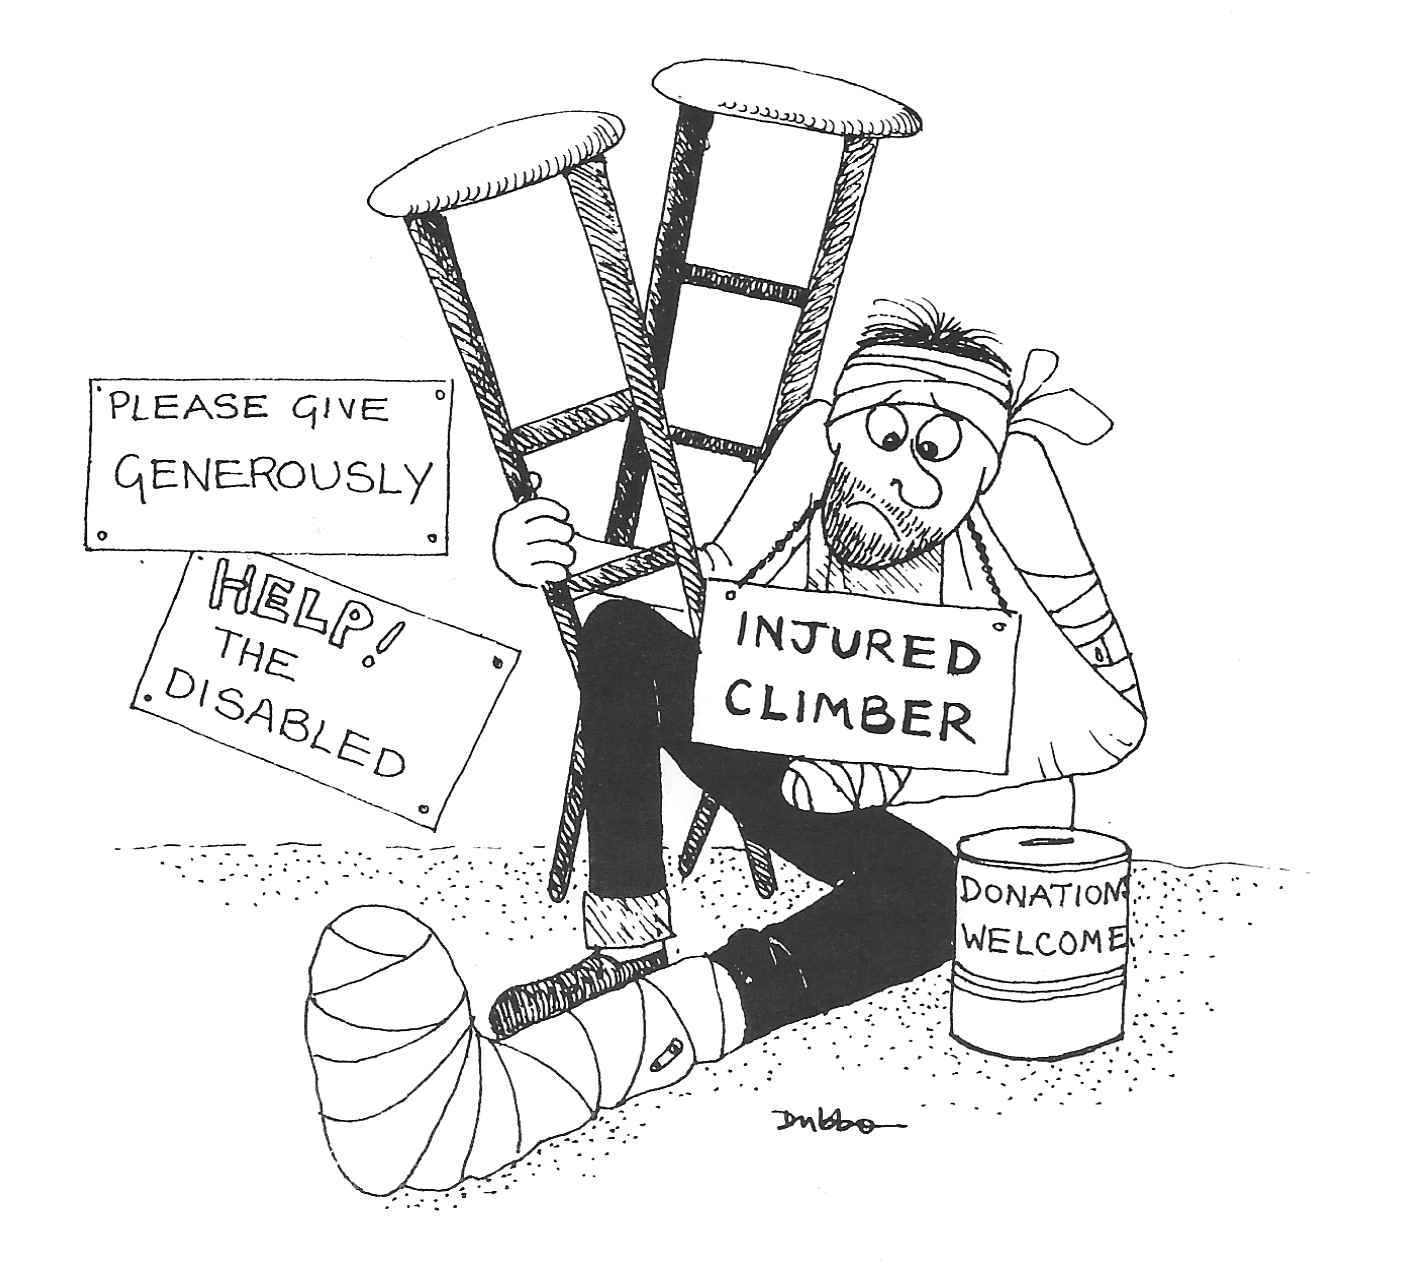
\includegraphics[width=.9\linewidth]{./images/Cartoon_09.jpg}
\caption{\label{fig:orge746825}
Falling Off}
\end{figure}

\chapter{One for the Pot}
\label{sec:orgbe80c0e}
\chapterauthor{Martin Whitaker}

Caving as a Club activity, first got on the official meets
list in winter 1983 84, though some members had "dabbled" some
years before when Geoff Tryon had organised a beginners' and an
advanced trip.

The first "official" trip, to Carl's Wark Cavern, was well
attended despite heavy snow in Sheffield, causing one car to have
an argument with a wall.

Conditions were wet underground and Steve Hartland led us
through a short low section where the immersion of one ear was
obligatory   great fun! We were out in time to get changed
 chilly in the snow  and go to the pub in Eyam for a lunch time
pint   all except Dunky who forgot his change of clothes and had
to drive straight home, only to be refused entry to his parent's
house  so legend has it  until he had stripped off in the garage.

After this success, the following winter saw two meets on
the list with trips to Giant's and P8. Since then there has been
at least one Club trip a year and a few members have got so keen
that they have used the excuse of "going caving" to avoid nasty
bog trots. However, there are still a few folks unconvinced of
the attractions of caving and the excuses for  not  going on caving
meets have ranged from "I'm frightened of lifts" through "I've
been caving with you once that's enough!" to "Not bloody likely!"
Some even prefer to go to a nice, warm climbing wall, to do a
twenty mile walk in the rain, or even to watch Ski Sunday in
front of the box. But you cannot really beat a trip underground
for sheer enjoyment, the peak of which is normally reached
belatedly, whilst clutching a hot toddy in the bath at home.

The point of least enjoyment is reached shortly after
leaving the cave and is characterised by the removal of wet,
muddy clothing or wetsuits in rather less than comfortable
temperatures and circumstances.

I can remember when Andy Smith during a particularly tight
squeeze had to strip off down to his undies in order to get
through. This was not the first time that Andy's size had created
problems, a classic example being his ascent of  Cave Climb  at
Chatsworth Edge. The finish of the route is very similar to
caving and involves clambering out of a closed chimney via a
small hole at the top. With his legs flapping, Andy's body was
well and truly stuck fast until Charles came to the rescue by
hoisting him out by his braces!

One of the most memorable Club trips for me was the January
'86 visit to Swinsto Hole in the Yorkshire Dales. The small but
elite !  team consisted of Marian Birkett, Dave Crowther, Mike
Doyle, Dave Pendlebury and myself. It was a miserable wet day so
we were cheered by the fact that we were not missing any
climbing! Less cheering was the sight of flooded fields, with
rivers and canals absolutely full to the brim   what was that I
had heard about the West Kingsdale master cave flooding to the
roof? And the warning in the guidebook that the exit through
Valley Entrance "sumps in wet weather"?

The plan was to abseil down all the seven or eight pitches
of Swinsto, pulling the ropes down after us   a trifle
committing! However, some precautions for our safe delivery from
the bottom were taken by Dave P and myself going into the Valley
Entrance beforehand and fixing a ladder down into the master
cave. I even went down it to see how much water there was in the
bottom: instead of the normal three or four inches it was about
two feet deep and moving at such a pace that walking upstream was
virtually impossible. Still, not to worry, we would be coming
downstream!

Back outside after fixing the ladder, we reassured the
others that the water was lovely and warm and that only a small
epic could be anticipated, then set off up the hill to Swinsto
Hole.

The cave started off as it meant to go on   wet! Straight
into a low, tight, stream passage and quickly to the first pitch
  an abseil down a waterfall! Then 900 feet of stooping and
hands and knees crawling in water, knee pads a definite
advantage! A short waterfall descent into a pool was followed by
a curtain pitch down another waterfall. It was interesting to
watch the different techniques employed by people as they
disappeared into the waterfalls in a welter of foam   Dave P.
used technique and control in an attempt to keep out of the water
as much as possible while Dave C. employed speed as his defence
against drowning. The problem was, the further down the cave we
went, the greater the volume of water!

By the time we reached the main pitch   two abseils, one of
fifty feet and one of forty split by a ledge   there was some
real force in the water. I abseiled first here as on all pitches
 the privilege of being leader!  and could not see the ledge at
all until I actually touched it.

A sort of weird of disco was danced by the team to the music
of crashing water in a sheltered recess at the foot of the main
pitch, in an attempt to regain some of the heat lost from
prolonged immersion. What we needed, obviously was an immersion
heater? Groan, groan!

Everybody got warmed up again on the next section   an
exciting stream passageway with rapids to clamber down, pools to
fall into and tight bits to squeeze through. Eventually we
reached the final chamber after our eighth abseil. Not far to the
master cave from here!

Off we went down the east entrance passage on our hands and
knees, through a low watery bit and on to a gravel bank. All this
I remembered from the last time I'd been here. What I did not
recognise was the sump, where the roof of the passage gradually
lowers to meet the water level. To cut a long story short, we
went back and forth along a section of the cave before the
correct route was finally located. Just enough uncertainty to get
the adrenalin pounding!

Back in the master cave, the water was flowing down a
veritable helter skelter channel. Mike and I leapt in and
vanished down the cascades before the others realised where we
had gone: I must take a rubber dinghy down there sometime, it
would be great fun.

One thing I'll never do again is to solo up a free hanging
Electron ladder with a rucksack containing 150 feet of wet rope
and several gallons of water!

Luckily the bit in the Valley Entrance that "in wet weather
usually sumps" had not: there was at least six inches of air
space!

Once outside, the fresh air was, as always, welcoming   even
though it was still raining. It was very satisfying to know that
the walkers would undoubtedly have got wet too.
\begin{figure}[htb]
\centering
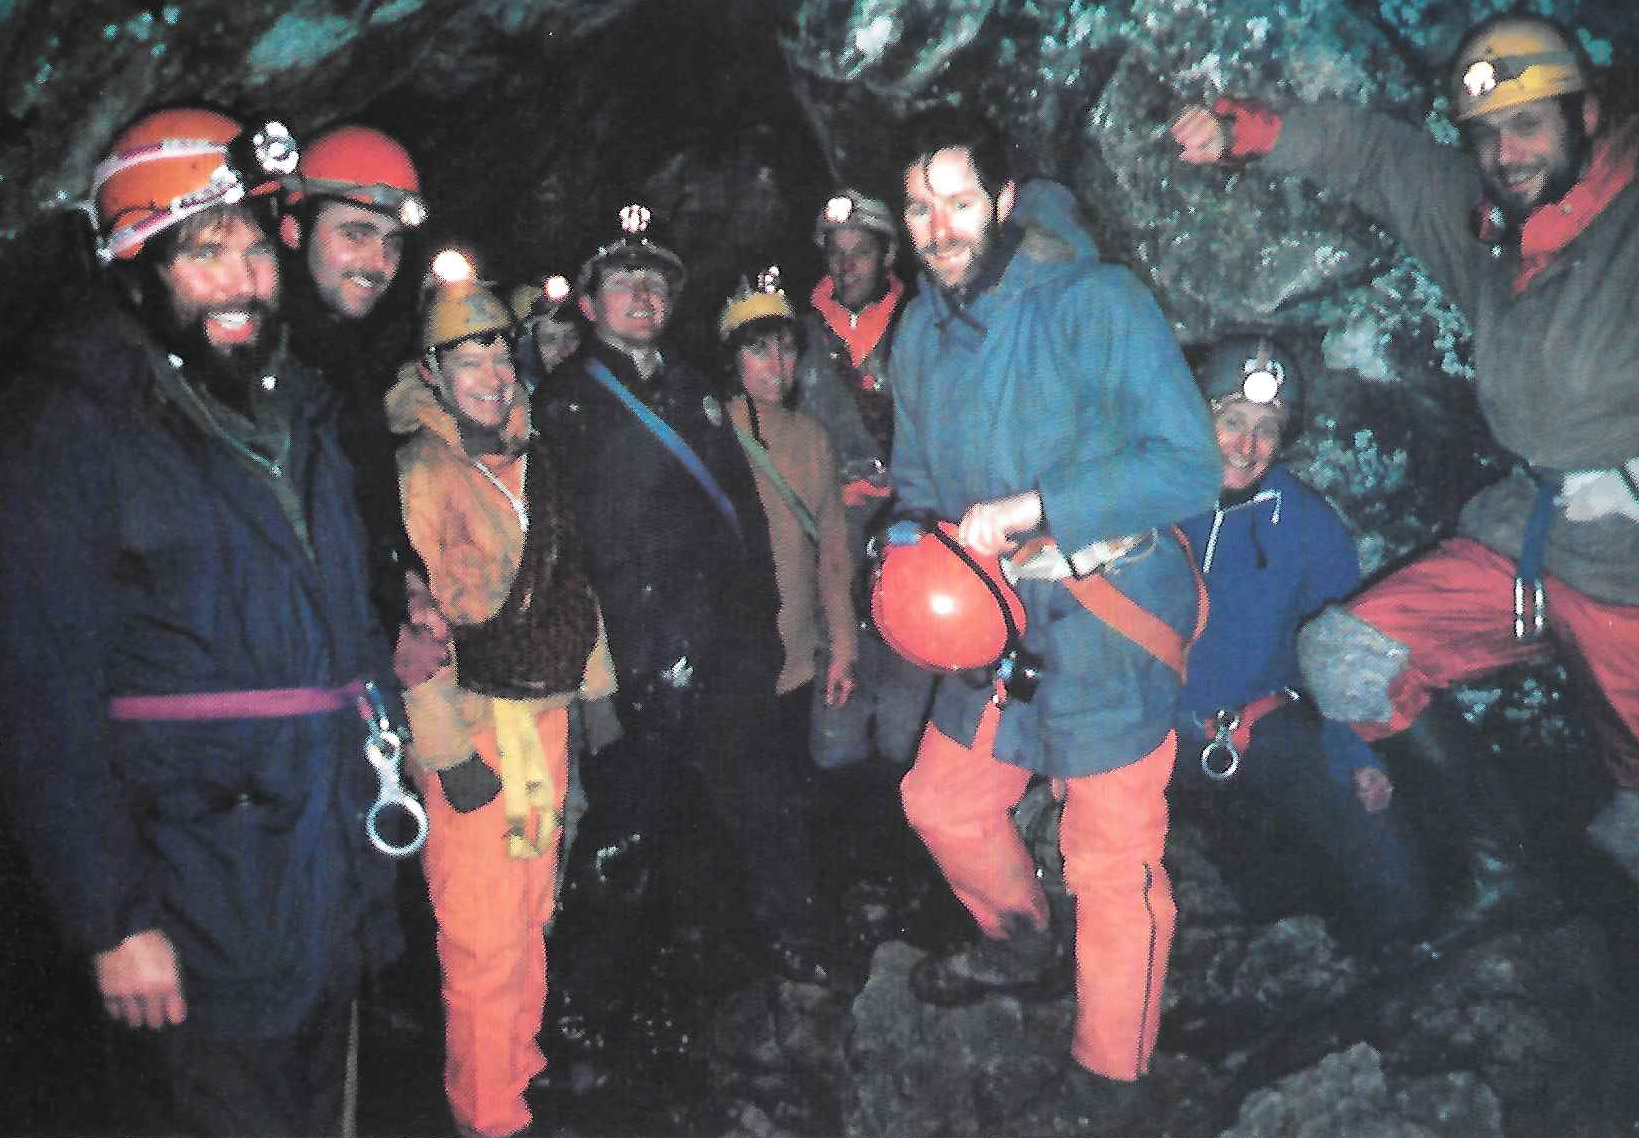
\includegraphics[width=.9\linewidth]{./images/Castle_Members_in_Giants_Cave.jpg}
\caption{\label{fig:org7186d7d}
Castle Members in Giants Cave}
\end{figure}

\begin{figure}[htb]
\centering
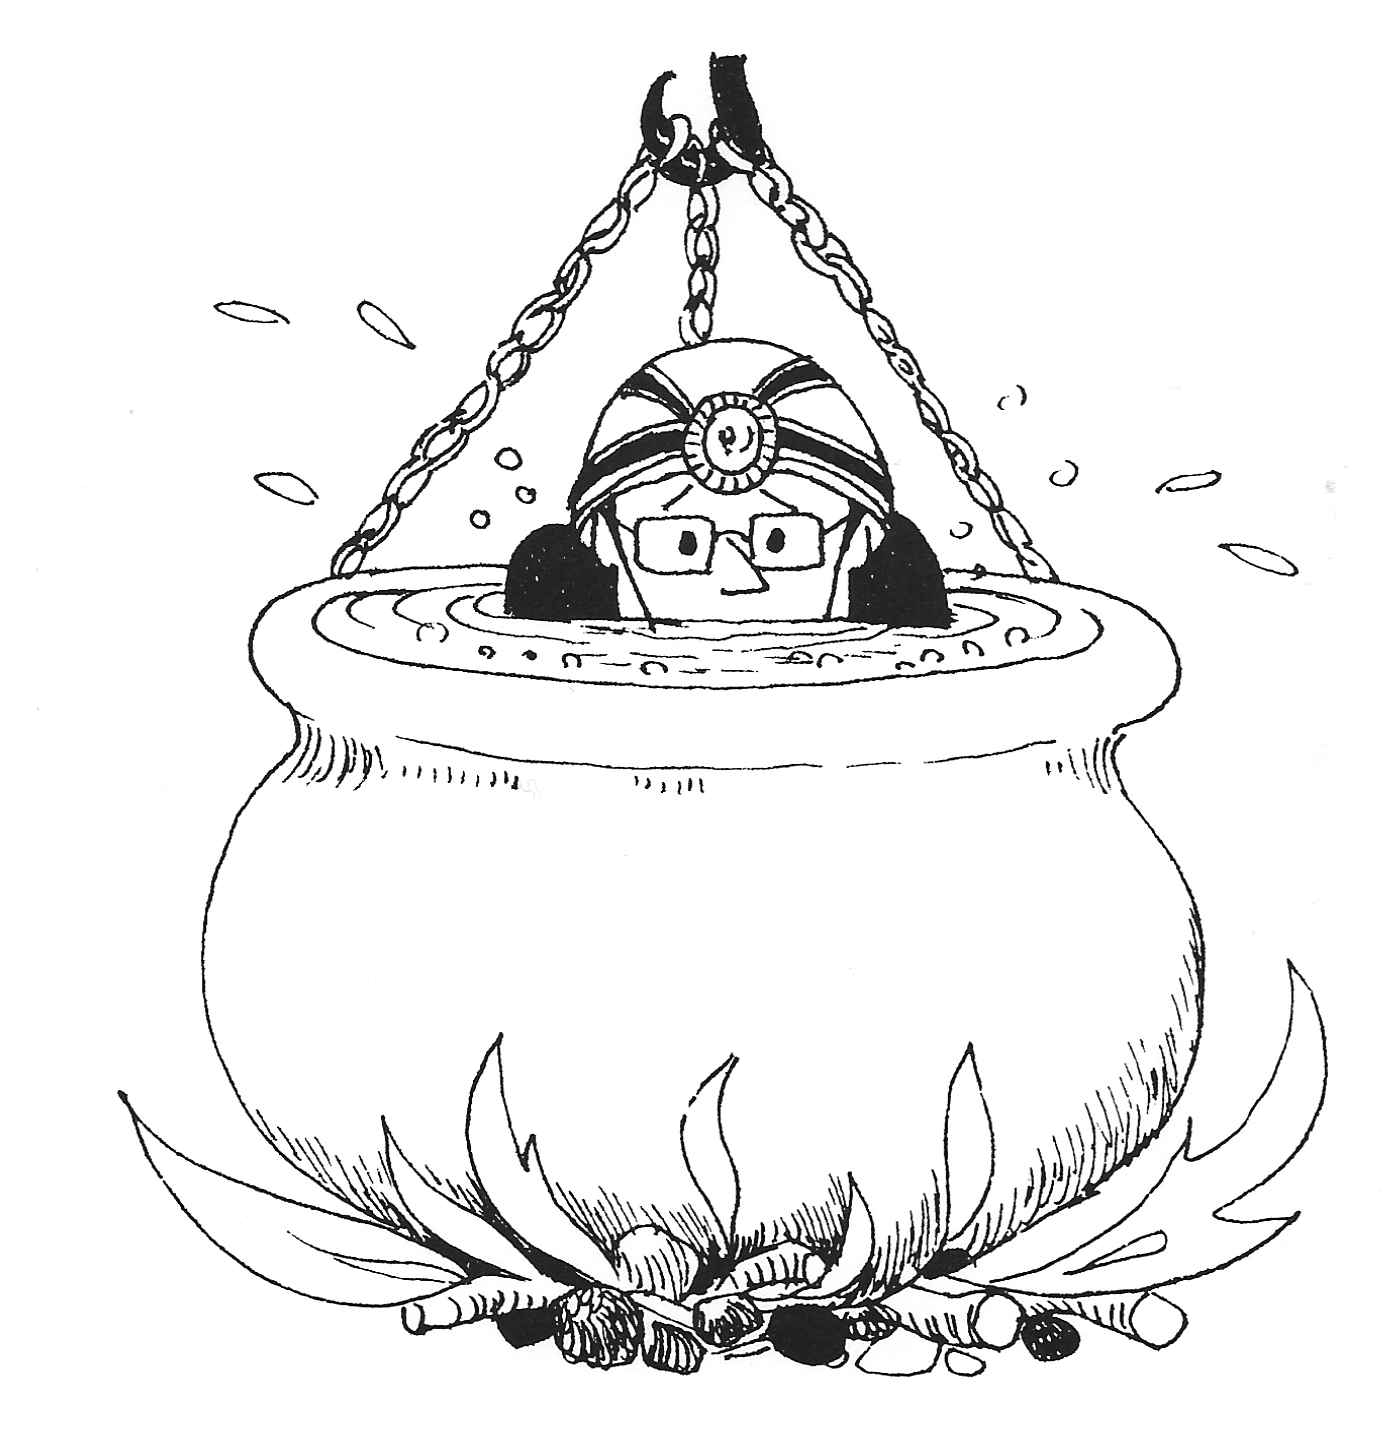
\includegraphics[width=.9\linewidth]{./images/Cartoon_10.jpg}
\caption{\label{fig:org95c3373}
One for the Pot}
\end{figure}

\chapter{Welsh Rarebit}
\label{sec:org5ca267d}
\chapterauthor{Steve France}

Bill Hine was spread out on the back seat clutching his
mouth in a desperate attempt not to laugh, as I stood outside the
car saying:
	"Yes Mr Policeman, No Mr Policeman, forty miles per hour I
think, Mr Policeman\ldots{}"

Chris Wright, sitting in the front, thought the grovelling
was far more entertaining than the car stereo so, turning it
down, he was just in time to hear:

"And I won't do it again Mr Policeman".

I entered the car soon after and shut the door with a clunk.
The resulting burst of laughter must have been overheard by the
rookie who was walking back to his police car.  His pride had
already been severely dented during his frantic efforts to catch
us up. However, the score was now one all and we were on our way
to Anglesey.

Since the opening of the M56, the journey is considerably
quicker than it used to be, but there's still time to reflect
back to those Welsh days when every route turned out to be a
classic or an epic adventure that gets worse every time you told
it.  A portion of my memory is always reserved for Idwal Slabs
and the mass ascents by the Club in big boots and cags.  The
Castle's hard core climbing team twelve years ago was a motley
crew led by Sheila MacDonald and her never ending fag and with
John Ward bringing up the rear, seen but never heard.  A few
years later some new faces came onto the scene and the climbing
grades started to rise to 5b 5c.  This was the time Bill was
introduced to the Castle  by Dave Bates and Keith Naylor  and
Dick Savage  Tricky Dicky  who was an earlier Castle climber left
for India to achieve inner transcendental harmony.  In those days
a Castle ascent of  Cenotaph Corner ,  Cemetary Gates  and  Vector  was
an achievement, but alas these routes along with many more have
been down graded to "just good classics". For me the mountain
classics will always hold that extra magic which the modern
routes lack at the moment. Maybe it's the atmosphere or could it
be just a pleasant memory?

All three of us in the car were quite adept at the modern
routes but on this occasion, after many months pestering, I
finally convinced Chris to have a go at a sea cliff classic for a
change. The car ground to a halt on the gravel surface of South
Stack car park. The air was damp due to the sea spray in the
blustery wind so that by the time we had our rucksacks and ropes
packed the "What am I doing here?" syndrome was setting in.

"OK, where's the crag?" asked Chris unenthusiastically.

After walking in a rough north easterly direction, for
twenty minutes, we were above the sea cliffs of Gogarth. Past
visits to the cliff had resulted in climbing the usual  Pentathol ,
 Gogarth ,  Cordon Bleu  and  Central Park  but unfortunately a large
proportion of the routes suffer from access problems during high
tide.  According to Sods Law, no matter what time you arrive it
will always be high tide! Today was no exception.  Reading the
Guide Book about high tide approaches was depressing and when we
consulted a group of "knowledgeable" climbers  who were festering
between some boulders they said, "You have no chance for at least
three hours". So, acting on this information, we set off to Wen
Slab. Maybe we could come back later or tomorrow but now a new
goal had raised our enthusiasm -  Quartz Icicle  or  Wen . Anything
except  Dream of White Horses , not because  Dream  is a poor route -
quite the opposite. For any first time visit it is highly
recommended, but I had climbed it three times before with
different parties and there had been no time left for anything
else.

On arrival it was decided to walk down the gully on the
right as you face out to sea for the spectacular view of the zawn
thus giving an impressive vista of all the routes. There it was
in all its splendour - Froggatt Edge on a Sunday afternoon in
summer! It was like Butlins Holiday Camp in the late sixties.
Quartz Icicle  was being climbed!  Wen  also! There were climbers
everywhere\ldots{} and no less than three parties on  Dream  alone! The
overall scene was stunning and very reminiscent of Baggy Slabs
with  Midnight Cowboy ,  Kinky Boots  and  Sexilegs   all being climbed
at the same time.

Chris was not impressed, as our only option was to trek back
to Gogarth and wait for the tide rather than wait for the crowds
to subside on Wen Slab.  Back we went, but this time we geared up
at the top of the descent path and climbed down the small gully
to the bottom of the cliffs. It was far better to wait here than
to brood at the top  at least we could look at the sea level
traverse and climb along at the earliest possible moment.

When we arrived it was high and dry by a long way, in fact
it looked passable at most times except for maximum high tide.
Our feelings were mixed: happy to be able to do at last the route
we had set out for and cheesed off because we had turned into
bigger pratts than the two "knowledgeable" climbers we met
earlier.

Traversing across the bottom of the cliff took no more than
a few minutes. The ropes were quickly uncoiled and we were ready
to climb  Big Groove .  Gogarth's  Big Groove  is not particularly
difficult by today's standards and rose to fame during the "Hard
Rock " days when its popularity increased tenfold.  Its total
height of 340 feet is climbed in three pitches of 5a 5c  and 5a
grading. Although this route had been climbed before by many
Castle members, for me it was the one that had got away.

Bill took the lead on the first pitch and burned up the rock
to disappear over a ledge some fifty feet up. Time lingered on
with relatively little movement from the rope.
	"Are you belayed yet?" I shouted, only to be met by silence.

The silence went on for some twenty minutes broken only by
the occasional jerk of the rope, until finally we heard the faint
call:
	"Climb when yer ready".

Chris set off and I followed some five minutes later,
puzzled by the apparent speed of his ascent, especially above the
ledge where the problem seemed to have occurred.

Upon reaching the ledge the puzzle became worse because Bill
and Chris were sitting only twenty feet away with no obvious hard
or even slightly difficult climbing between us. However, there
was a seagull!

"Don't disturb it, its nesting" whispered Bill, looking
quite concerned that I might kick it off.

In fact, as I was traversing an absolutely desperate wall
over the gull I did feel like kicking it off, especially when all
it could do was look up at me with a "look at that silly bugger "
expression on its beak!

Once on the belay ledge my immediate attention was on the
second pitch that I was about to lead. From the stance, very
little could be seen apart from the seepage lines of wet rock,
with the mist and sea spray blowing up the groove. I was unable
to convince Chris that this was the pitch he ought to lead, so I
set off. A short wall led to the groove itself which was
deceptively steep. In fact it gets steeper each time I think
about it! I must confess that I'm not a particularly strong
climber and I usually try and make up for that deficiency by
technique  however, that does not always work, especially on
routes like  Axle Attack  and  Body Machine  where without strength
and stamina you just don't stand a chance of a clean ascent.
Anyway, by now the groove was seeping with water and had got
very, very, steep   even steep enough to justify my owning up to
using the peg! But it was only for a few seconds, honest!

I knew that hesitation below the peg would prove disastrous,
because slowly but surely my forearms were beginning to ache with
their solidification.  The veins pulsed and stuck out like
fossilised tree trunks, to be shortly followed by the involuntary
uncurling of the fingers.  With one last effort I managed to
reach the bottom of a flake, and thrust my fingers right round
it, preventing them from uncurling. How many times do you get
into the situation when you're twenty feet above your last
protection, pumped out of your head and the flake does not allow
the insertion of any useful gear?

The only option was to continue up the flake where it formed
an apex and lasso a sling over it.  What sounded like a good idea
turned out to be a nightmare, as I laybacked up the flake higher
and higher until the last runner was just a distant memory.
However, there was one consoling factor - if I fell off now there
would at least be a strong possibility I would land on that gull!

Almost there, but something didn't seem right. Could it have
been the groaning and creaking of the flake? After some thought I
realised that the whole flake was bending and flexing with every
layback thrust. Nervously peering round for a closer
investigation, I saw the true thickness of the flake to be only
half an inch.
	"It must be stronger that it looks, having remained on the
route for so long" I thought, in a desperate attempt to convince
myself that everything was just great.  Lassoing the tip of the
flake with a sling, I remembered the verse by Ben King:
	"Nowhere to fall but off, Nowhere to stay but on."
	What a load of garbage!

The karabiner clicked home and the tension eased as I boldly
bridged up to the right below the belay stance and heaved my body
onto a ledge. Standing up on the ledge was another matter but the
whole performance is too embarrassing to describe here. The ledge
was just right for one, and when Bill arrived soon after it was -
for want of a better word - "cosy".  When Chris arrived, however,
the ledge became a writhing mass of arms, legs, ropes and
runners.

Chris had intended to lead through but the weather had
turned increasingly nasty. Over the last hour, during the ascent
of the second pitch, the clag had set in and spray was howling
upwards in the vortex created by the groove. The whole effect
made it look as though it were raining upwards!  The decision had
been made earlier that if I managed the second pitch we would go
on, but if not we would abandon the route. Unfortunately there
was no turning back now.

Chris set off up the final groove very slowly, as by now
everything was totally saturated, even Bill and I. Rather than
start singing "My favourite things" I began to think about
sitting in front of a roaring open fire in the pub that night,
swilling the amber nectar and talking of the day's events
especially giving Bill a roasting for wasting a good hour by
being polite to the seagull!

By now we were well and truly frozen stiff with all
enthusiasm long gone. The rope very slowly came to its end and
assuming it was time to climb, I set off. I must admit and said
to Chris at the time that his lead on that final pitch in the
conditions that prevailed was superhuman. The fact that he
managed to stay on at all is beyond me - let alone climb the
soaking lichen pads and shattered rock flakes.  At long last, the
top was made by all three followed by the quickest descent  via
the path!  on record.

There was no fire in the pub but there was a pool table
well, you can't have everything.

\chapter{Two Weeks Older, Years Wiser}
\label{sec:org282fe4a}
\chapterauthor{Claire Coates}

Sitting in the warmth and comfort of my home, Alpine
adventure seems very far away indeed. Knowing the tricks that
memory and time can play, on countless occasions in the Alps last
summer I told myself sternly and fiercely, often through hot
tears:
	"You will remember how evil this feels. You will remember
that it's sheer hell."

I was very naive and unsuspecting when I left for the Alps
for the first time the previous July. Excited and apprehensive,
yes, but sure of myself. I knew the environment was dangerous
but, after all, I had prepared very carefully, I had trained, was
as fit as I had ever been in my life, had good safe equipment and
was to be coached through my first Alpine experiences by a
professional guide. I was looking forward to it very much.

I travelled out a few days early so had some time to spare
before I was due to join the guide. The campsite at Argentiere
had a lively, British, climbing community and those first few
days were easily filled, walking and climbing with new friends
and getting used to the Alpine scale of things. With two people
from the Red Rope MC I climbed the  Papillons Ridge  in fine
conditions, thoroughly enjoying the stunning positions and
interesting rock climbing. The altitude caused no problems,
neither did other first experiences like climbing with my
rucksack and long abseils. We had a long walk off the mountain
because we missed the last telepherique down to Chamonix, but it
was a delightful walk along green paths, made even better by
eating wild raspberries and listening to booming rock music
echoing up from a concert in the town below. It was a sound and
optimistic beginning.

My guide was in fact the only British woman qualified as a
guide, well respected and with a great deal of experience of
Alpine courses. She worked with Tim, a good, strong climber who
also knew the Alps well. The two people in the group with me the
first week were a married couple, Karen and Kevin, who had walked
in the Alps before but had little climbing experience. The second
week we were joined by two men with a burning ambition to reach
the summit of Mont Blanc  nothing else, just that. John and Ron
had virtually no experience of any climbing and I had never set
foot in the mountains on snow or ice before. A challenge to the
sturdiest of teachers, I would say! Little did we know what fate
had in store for us.

We began our training on the Mer de Glace. Those of you who
are familiar with Chamonix will know that there is a perfectly
good train which takes you  and hundreds of tourists  to
Montenvers, only a short walk from the glacier. But for us,
walking was not to be shirked. What's more, I foolishly wore my
new plastic boots   personal torture chambers which pull you down
with every step and slowly pot roast your feet. By the time we
reached the glacier, what with the boots, a rucksack that was far
too heavy, the steepness of the hill and dehydration, I felt as
if I were going to die. It was a sensation I was going to get
used to. Donning crampons for the first time, I felt about ten
months old, learning to walk again. Small, tentative steps,
scowling at our guide when she shouted at me to jump around.
Then, in order to practice, we walked unroped around the glacier,
picking our way over crevasse bridges, up and down slopes   very,
very, slowly. Fear seemed to have stolen my sense of balance. We
stopped to do some rope work and learn safety techniques,
including crevasse rescue. One by one we played rescuer and
rescued. Weighing much less than the others, it seemed at times
that my legs and back would snap. I moaned, a lot.

I was encouraged because for the next couple of days we were
to leave the ice and turn to rock. We did two long routes on the
Massif des Aiguilles Rouges, bivvying overnight at the Index
station. At this time there was very little snow and the normally
snow covered gullies were full of hot, broken rocks which took
you sliding back as you tried to make upward progress. Soul
destroying. Back breaking. Painful. The rock climbing was sweet
release, technically easy and in fine weather. At the end of the
rope I was left to my own devices and I enjoyed the marvellous
views and some relaxation.

Following this, on our fourth day we set off for the snow,
planning to do the Petite Aiguille Verte on the way to the
Argentiere hut. Unfortunately I was struck with altitude sickness
on the ascent and had to be left sitting on a rock in the hot sun
watching enviously as the others went on up to their first "snow"
summit. The sickness became worse and I made the arduous trek to
the hut feeling only semi conscious and in need of a great deal
of support. Staying in the hut brought more new experiences   a
whole new regime. There was so much to remember, like getting
water for the next day in case the pipes froze overnight and
arranging your gear so that nothing was forgotten or lost. I was
thrown into a permanent state of panic.

At 3 am, a gentle whistle roused our dormitory and,
bleary eyed, we prepared for the day. It took us forty minutes and our
guide was furious   we would have to manage in a third of the
time in future! So, late, we set off for the Aiguille Tour Noir.
Before long, unable to keep up and still feeling sick and dismal,
I lost sight of the others. I had come to the Alps hoping to
learn to love the mountains and I was beginning to hate them.
Once again I was left behind, this time in pitch darkness and
freezing cold, waiting for dawn so that I could safely return to
the hut and all the while wondering if I could afford the air
fare home. I felt a mixture of disappointment, frustration, anger
and fear. But if I thought that I would be let off that lightly,
I was wrong. The next day we were marshalled swiftly out   I
think I slept in everything except my glacier cream   and even
did without a drink or a visit to the toilet to be ready in time.
After much faltering, cajoling, complain ing and encouraging, by
mid morning I had reached the summit of the Aiguille
d'Argentiere. What an enormous sense of relief and achievement. I
didn't want to go home any more.

The elements then decided to intervene and we had two days
of continuous torrential rain, which meant one day's rest and one
day in a flood on the Bossons glacier, trying to front point up
the steep sides of crevasses as water poured down sleeves,
gloves, trousers and socks and lightning cracked around us. Only
when we had achieved what we had come for were we allowed to
retreat to the Bar Nationale. Once down to the car, I incurred
our guide's wrath and a new reputation by removing all my clothes
at the roadside. Dry clothes seemed worth any consequences.

We spent the next night at the Albert Premier hut and
although a snowstorm delayed our start we conquered the West and
South Summits of the Aiguille de Tour. After a great day rock
climbing at Les Gaillands, which reminded me of home and restored
some confidence, we set off for our last expedition. We were to
do part of the Midi Plan, bivvy in the Midi station and tackle a
final route on the morning of the day we were due to travel home,
leaving Chamonix at noon. Quite a schedule.

There had been extremely heavy snowfalls up high   the
 Papillons Ridge  I had rock climbed only days before was covered
in snow. With hindsight, we should not have attempted the Midi Plan
in those conditions, with deep snow blocking the normal
route. We soon ran into trouble, confronted by difficult,
technical, rock climbing in full ice gear. It was a traumatic and
dangerous time, ending in an abseil escape and retreat to the
Midi station. This experience played a large part in my choice of
route for the following day. Half of the group was to tackle the
the Cosmiques Ridge , whilst Tim would do Mont Blanc de Tacul. I had
no desire to repeat the events of the Midi Plan and was very keen
to climb over 4000m, so I chose to go with Tim. We had a
magnificent meal in our comfortable bivvy and enjoyed a superb
sunset. Spirits were high.

At 3 am Tim, Ron and I set off, leaving the others
sleeping. The ascent was marvellous. By this time I was beginning
to get fit enough and we progressed quickly, leaving two parties
from Cardiff University in our wake. Despite the deep new snow we
were on the summit before 7 am, accompanied by a very spectacular
dawn. I felt on top of the world. Beginning our descent, we
passed the other British groups and reached the top of the main
slab.

Imagine making your way gingerly down a narrow ice ledge,
balanced on crampon points and ice axe, expectantly working your
way towards the safety of the snow slope. And then\ldots{}\ldots{}. that
slope moves, lifts itself from the face of the earth and hurls
itself down the mountainside. Half a mile of snow, at least
twenty feet deep, suddenly erupting, causing a thunderous roar.
Nothing in the path of that avalanche could have survived. It was
a monster. A monster no more than fifty feet away. Tim screamed
at us and literally dragged Ron and myself back up the ice ledge
away from the chaos beside us. I have never, ever, been so
frightened.

But the trauma had only just begun. How were we to get off
the mountain? As we stood debating the horrific options with the
other groups who had reached us by this time, a French policeman
was dropped from a helicopter. His interest, understandably, was
to discover if there had been anyone on the slab. Miraculously
there had not. He offered no advice as to our descent   we were
the mountaineers he said, we should tell him! He would be willing
to pick up our bodies if we risked triggering another avalanche
on the cracked and unstable slab, but he was not interested in us
alive. Fortunately common sense prevailed. It had been the
largest avalanche of the summer there and to have had to deal
with nine British bodies would have been inconvenient. So, the
helicopter came back and in circumstances that seemed more
appropriate to the television screen, we were whisked from the
mountain top to the valley.

The weird helicopter flight which seemed to turn the world
upside down and the sight of rescue workers  and dogs on the mass
of broken snow brought home the awful reality of it all and I
cried and cried. We should have been dead. Hesitat ing on the
summit for a final photograph, stopping to adjust my crampon,
moving so slowly on that ledge   the reasons we hadn't been swept
away came back to us in the sudden realization of what might have
been. We had to walk from the Vallee Blanche back to the Midi
station, interrupted mid way by another policeman, dropped from a
helicopter with more questions. The other party, who knew we had
reached the summit because they had watched our head torches in
the early morning, had witnessed the whole affair but could not
know we were safe until we arrived back. Their relief was almost
as great as ours.

I was glad to say goodbye to the Alps. They had been hostile
and frightening for much of my time there. I had felt bullied and
lonely and longed for the security of The Peak District, my home
and friends. Without pressure from our guide I would undoubtedly
have given in many times to physical discomfort and cowardice. As
it was, we had achieved an incredible amount in the time
available. Despite the aggressive conditions, I had learnt and
achieved more than I had thought possible   about climbing, the
mountains and most of all myself, what I am capable of and what
my true limitations are. For the future I know I must be
stronger, fitter, more determined and more self reliant to
survive in the mountains, and even then it will still be hard. I
have just finished reading "The White Spider" which chronicles
the savage history of the North Face of the Eiger. In spite of my
experien ces in the Alps I felt inspired and challenged by those
awesome tales, not intimidated and frightened. Perhaps those
tricks of time and memory have won after all. Or perhaps that's
the magic of mountaineering.
\begin{figure}[htb]
\centering
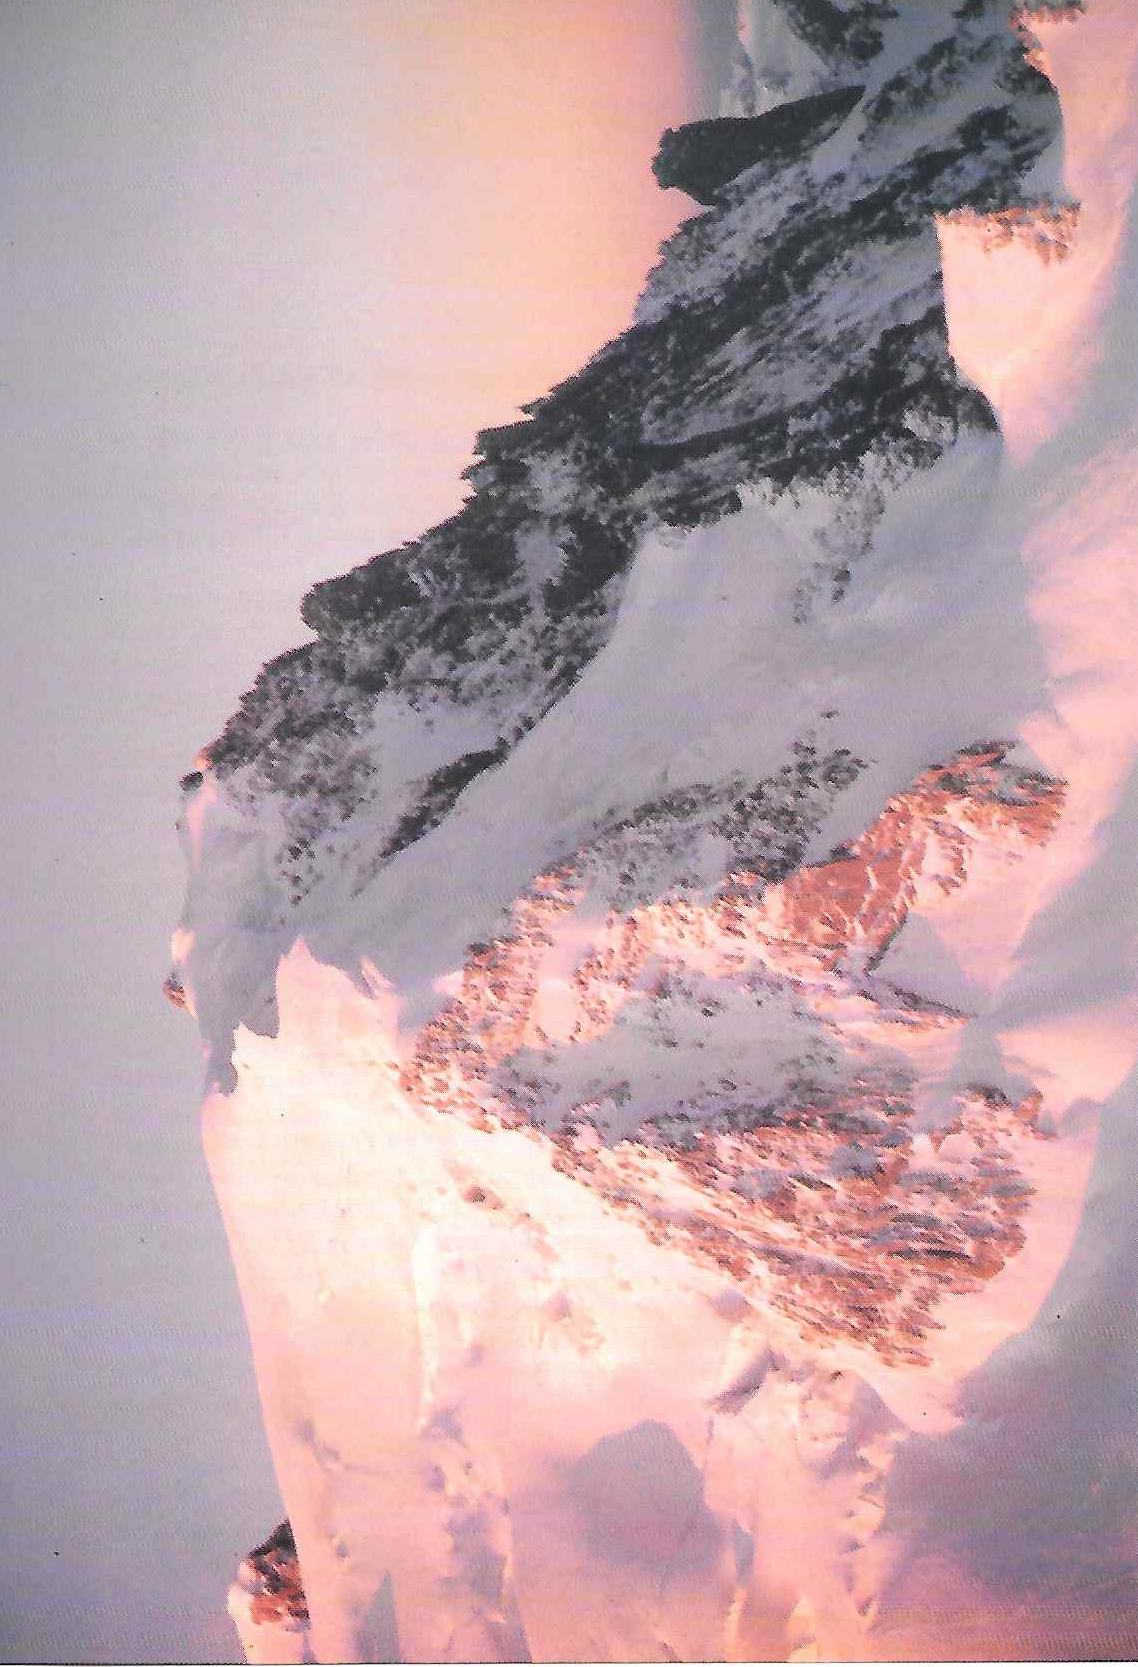
\includegraphics[width=.9\linewidth]{./images/Mon_Blanc_de_Tacul.jpg}
\caption{\label{fig:orgb6e0ac9}
Mont Blanc de Tacul}
\end{figure}

\chapter{Death Race 2000}
\label{sec:org4d0ff85}
\chapterauthor{Steve Ralph}

"The Karakoram Highway is like a cassette tape strewn across
a building site"   Robin Dennell.

We stood on the side of the road. Our driver was on his back
at the front of the vehicle with only his legs protruding. We
wished that he would fall asleep and stay asleep for at least
another four hours, but our hopes were dashed by the occasional
grunt and the tinkle of a spanner.  Our driver was of the opinion
that no sleep for two days was no problem.

Brightly lit vehicles moved up and down the artery, the
vivid patterns on their flank like an arcane genetic code. A
thousand or so feet below, the waters of the Indus waited
greedily for a driver to make one last mistake.

The second vehicle arrived, and within minutes the wheels
spun on the gravel creating a huge dust cloud which attached
itself to the back of the van.

One hour from Islamabad there was a crunch and it broke
down. As the driver walked back to Islamabad to get a part, we
went in search of breakfast but found a Buddhist Temple instead.
The Moslems had knocked the heads off the Buddhas. Even though we
didn't look like Buddhists we decided not to take any chances and
beat a hasty retreat. Apart from that,temples didn't do eggs. The
culture shock was setting in. After little sleep on the plane and
only a day in Islamabad and the British Embassy Club, we had
hardly acclimatised.

Our driver returned with a new transmission link and we knew
that this one was OK because it did not have a welded fracture
down the middle. We progressed towards the mountains, through a
strange land where everybody wore the same clothes and there were
no women in the streets and it was even hotter than Skegness. Our
driver's techniques in built up areas began to arouse our
interest. Foot on accelerator, hand on horn, it is the Will of
Allah if you don't move out of the way.

After a tea stop in a place called Beshum, things changed
abruptly. The road along the bottom of the pleasant valley, with
steep crumbling sides above, suddenly became the road half way up
the mother of all gorges, with steep crumbling slopes below. The
road twisted and turned like a demented python. Our driver's
cornering technique  foot down, horn on\ldots{}  began to cause
serious concern, as did his tendency to race anything that
overtook. Occasionally he would stop, point down and say "Ten
men" or "Five men". I wondered why we were never driven over the
edge of the Karakoram Highway.

The Indus gorge is huge by European standards. The initial
section of the Highway travels up this immense feature for maybe
a hundred miles. It has a distinctly temporary  in geological
terms  feel to it and at many places we encountered landslips.
Time has used the sharp blade of the Indus, swollen with glacial
melt, to slice through the moraine rubble, leaving a great chasm
to drain the Western Karakoram. Then somebody decided that a road
along its walls would be a good idea.

Respite came at last when we found ourselves at a village.
We stopped and went into a restaurant.
	"Ah" said Uncle Tom, "It's the restaurant at the end of the
Universe."

We ate our curry and chappaties. The curry was delicious.

We set off again  foot down, horn on\ldots{}  We told our driver
to drive more slowly. He agreed   and promptly accelerated. The
next hour is indelibly etched in my memory. The Highway has a
grand rhythm. An experienced driver senses the rhythm and will
drive safely at a good pace. Ours was simply going too fast. The
motion was becoming unstable. Each swing, each last second
braking, each overtaking, brought us closer to the point of final
instability. Somebody's comment, that with a good launch we could
expect between five and six seconds of free fall before impact,
did not help. The drop to our left took on the aspect of the
Reaper's Scythe. Each of was in a private hell, convinced we
would never see our beautiful peak, let alone climb it.

"Slow down," we shouted.
"Yes," he cried   and accelerated again.

We careered round a double bend to meet a lorry like a squat
brightly coloured bug coming towards us. The resulting manoeuvre
made the back of the van drift. The string snapped and as one, we
leapt up in our seats screaming "STOP!" He refused.

Suddenly there was an awful noise from the back. Rickets,
the retired  at twenty one  coal miner from Barnsley was
obviously in severe pain. His features contorted, he grasped his
stomach in agony and made awful retching sounds. This did finally
convince the driver to stop. Rickets recovered suddenly and leapt
out, quickly followed by the rest of us. Things got very fraught
when we refused to travel any further until the driver had rested
\begin{itemize}
\item it emerged that he hadn't in fact slept for two days - and he
\end{itemize}
said he was going on with or without us, as he consumed a huge
lump of local "medicine".

Eventually we reached a compromise. We would travel in a
lorry we had flagged down and the van would travel behind us. Our
friend The Survivor, being brave, would stay in the van for
security's sake. Ten seconds after starting, the van overtook and
the Survivor screamed for help out of the window with a pleading
look on his face.

"No worry" said the lorry driver, "Soon he sleep."
We enquired as to the source of this insight.
"We gave him opium cigarette!"

A few miles later we found a shaky Survivor, a van, and the
driver trying to mend the fan belt with a piece of string. This
is in fact impossible, but he refused to be beaten. A spare from
a passing van eventually cured it. We were leaving the gorge now
and entering a strange desert plateau, ringed with arid mountains.
The free fall time was now down to half a second but by
now we were too numb to feel any terror.

Eventually he pulled into the side of the road.
	"I sleep."

He was out for five hours. We dozed in the desert, watching
the miracle of the dawn we had scarcely expected to see.

Arriving in Gilgit we parked in the main street. A fierce
man came towards us and grabbed the driver by the throat. He
dragged him out of the cab and the last we saw of him was his
being punched and kicked down the street. The fierce man returned
and drove us carefully, sedately and with consummate skill to the
refuge of the Hunza Inn. The story of how the Sahibs had gone on
strike had travelled on ahead of us.

Well, Rickets and his climbing partner The Cowboy made the
first ascent of our beautiful peak and The Sheffield Karakoram
Expedition was a resounding success, but that is another story.

\chapter{Island Flings}
\label{sec:org683055d}
\chapterauthor{Mike Doyle}

Islands hold all sorts of fascinations although for some more than
others and for me more than most. The Castle Mountaineering Club has a
climbing interest in the Scottish Islands of Arran, Rhum and Skye and
these islands therefore feature frequently on the Club's summer meets
list. In my case, a keen interest in islands has become an obsessive
urge to visit ever remoter, wilder and far flung spots. I am, though,
wary of the D.H. Lawrence tale "The Man Who Loved Islands" in which
the subject of the story, seeking ever smaller island sanctuaries,
finally retreats to a slab of rock from which he is swept clean away.

My interest in islands began in Easter 1974 with a visit to Arran. The
trip involved leaving my then base of Reading at five o'clock on
Maundy Thursday evening, travelling to Bristol to collect one member
of the team and and then undertaking a further journey to Stoke on
Trent to collect two other members, followed by a run to Ardrossan and
the early morning ferry to Arran. The return was equally frantic and
saw me back at my desk at nine o'clock on Tuesday morning. In between,
however, was an experience of true island bliss blue skies, anti
cyclonic weather, a snow capped Cir Mhor and vistas of the west coast
of Scotland and the nearby Paps of Jura. It was a three day glimpse of
paradise that started a permanent island obsession.

Having whetted my appetite with the benign and accessible beauty of
Arran, I began looking for more demanding locations, preferably those
with mountaineering potential. A timely move to Sheffield and
subsequent membership of The Castle Mountaineering Club certainly
helped. Mull, Skye, Rhum and Jura became obvious
choices. Unfortunately, I arrived in Sheffield with too little time
spent in my new employment to have earned a week's holiday and
therefore felt obliged to remain south of the border whilst the Club
trip to Skye in May 1975 went ahead. That was the year Skye wilted
under a week long heatwave and much serious climbing was done
including a Club traverse of the Cuillin Ridge. All I could do was
seethe with rage on learning what a good trip I had missed.

The following winter I learned that the Club was planning a Spring
Bank Holiday meet on Rhum, but I was again unable to join the
trip. Rather than miss out altogether, I obtained permission to camp
on the Island at Easter and so got there in advance of the main Club
expedition. I shall never forget the feeling of commitment at the
sight of MacBrayne's ferry steaming away, leaving us ashore with only
the tents and the food we had taken to sustain us for the coming
week. A week of gales, leaking tents and wet sleeping bags took away
some of the initial gloss, but the experience of watching deer only
feet from our tent and an ascent of Askival on the only day of
brilliant sunshine with views of the Cuillin on Skye, the nearby Small
Isles and more distant Outer Hebrides shimmering beyond the deep blue
Minch, easily compensated for the grimmer times. I was, though, left
with a slight "niggle" when the subsequent Club trip in the Spring
again found good weather and members packed in the routes.

The Rhum experience led me to visit a series of small and remote
islands where the attraction was the intrinsic interest of the island
itself rather than any mountaineering opportunities.  Thus it was that
I arrived green and seasick in North Haven on Fair Isle after two
hours tossing about on the sea on the Island's mail boat. Ignoring the
obvious mountaineering and swimming!  challenge of Sheep Rock, I was
enchanted by the peace, abundant wildlife and cheerful simplicity of
the fifty or so human inhabitants.

Thoroughly "hooked" by now, I spent a fortnight ploughing the
Hebridean waters helping as crew on a seven berth yacht.  Twice it was
nearly all ended: first by a scrape with an unexpected overhead power
cable on the west coast of Lewis and secondly by a navigational
blunder that led us late at night into an uncharted bay at the
entrance to Stornoway harbour.

Through this island touring, I eventually developed an obsessive
interest in a small, remote and hard to get to island group beyond the
Outer Hebrides. I mean of course "The Islands on the Edge of the
World" as they were once described, or St Kilda by their present
name. I first noted them with little more than idle curiosity as dots
on the map, but then I read an article in a climbing magazine which
aroused my interest. The description of the highest sea cliff in
Britain and the largest gannetry in the world, surrounded by Atlantic
seas, drew me to these islands like a magnet. The sad story of the
former occupants of the islands, their fate at the hands of
"civilization" and their ultimate evacuation added human interest.

However, my attempts at getting there were singularly
unsuccessful. Twice The National Trust for Scotland rejected me as an
applicant to join a work party, and an attempt to sail there by yacht
had to be abandoned in high seas. The more my attempts to get there
failed, the more I became obsessed with these Islands and the more I
redoubled my efforts to find a way to cross that elusive forty five
miles of Atlantic Ocean.

Eventually my patience and perseverance triumphed and I did duly set
foot on the shore of Village Bay on Hirta, the main Island. Here at
last was a remote island, well out to sea, out of sight of land and a
truly wild place. The teeming sea bird life was ever present, the wind
and sea pervaded all nooks and crannies and the drama of the cliffs
was mind blowing. Yet amidst all this drama the old village and the
old graveyard peacefully enhanced the natural appeal of the southern
sweep down to the sea of the Island's highest point, Conachair.

It was with a heavy heart that I bade farewell to these lonely and
spectacular islands and returned to mainland Scotland.  There have of
course been other islands since and I have more targets for the future
for example Foula, reputedly the St.  Kilda of the Shetlands. Perhaps,
though, I should try further afield. A glance at the shattered
coastline of Norway also looks promising, with gems like the Lofotens
very appealing and rekindling the old mountaineering spirit. Yet the
lure of the Scottish Isles is hard to shrug off and once again I shall
find myself setting off to the Hebrides. Although I shall be
trespassing rather close to the Corrievrecken whirlpool, there are
hopefully sufficient reasonably sized islands around to avoid my
resorting to slabs of rock and experiencing the watery grave warned of
by Lawrence!

\chapter{La Grande Epique de la Petite Dent de Veisivi}
\label{sec:orgd414c7f}
\chapterauthor{Les Alpinistes Poetiques}

A cautionary tale of the Western Pennine Alps, to be read
aloud in an accent appropriate to that well-known Russian
Yorkshireman  pretender to the throne , now resident high
above the Arolla valley, Aiguille de t'Csar.


\begin{verse}
\vspace*{1em}
"The Dent de Veisivi's an excellent climb"\\
Read JB from out of his book\\
"If we do it tomorrow there'll be plenty of time\\
To get back to the campsite and cook."\\
\vspace*{1em}
At quarter past nine we started our way,\\
By nine seventeen we were lost\\
The path on the map was as clear as the day,\\
But not on the ground  to our cost .\\
\vspace*{1em}
We swarmed up a gully that were filled up with boulders\\
To get to the path at the top\\
The sacks on our backs were hurting our shoulders,\\
So we thought it were time for a stop.\\
\vspace*{1em}
We had our first lunch-break at quarter to ten,\\
The second at ten forty-four.\\
We were nearing the col by two, but by then\\
We had needed to have several more.\\
\vspace*{1em}
We had planned the classic Veisivi traverse,\\
But JB felt a need for his bed\\
And the weather was making a change for the worse,\\
So we took the direct route instead.\\
\vspace*{1em}
JB having gone, there were five of us left,\\
So we put on our boots and the rope.\\
The rucksacks were stowed in a deep rocky cleft\\
And we carried on climbing the slope.\\
Dave rounded a corner to find a wide path:\\
There were goats and a firework and all.\\
"Oh heck, I'm embarrassed", he said with a laugh,\\
"We don't need the ropes here at all!"\\
\vspace*{1em}
But Dave was quite wrong - as we later found out -\\
For he scampered the ridge with much glee.\\
Then he looked up in terror as he heard Maxi shout\\
"'Ere, this side's as loose as can be!"\\
\vspace*{1em}
Dave soloed on up to check out the top\\
And were about to turn back when he saw\\
A bright shiny peg there gleaming in t'rock,\\
And he thought, "I'll have that for sure".\\
\vspace*{1em}
And once on the top Dave discovered\\
The route we'd been missing all day.\\
"Our fortunes can now be recovered,"\\
He said, "by going back down the right way."\\
\vspace*{1em}
Like sheep the rest of us followed,\\
But the last of us had to beware:\\
"I'll clean up this crag", Maxi hollered,\\
As he threw half the face to Haudres.\\
\vspace*{1em}
Person by person we reached the summit,\\
Each shivering down to the bone.\\
The guidebook descent was a plummet,\\
So we chose a new route of our own.\\
\vspace*{1em}
It were Max that found the creaky old post,\\
Which he said, in his judgement, were sound.\\
And by total agreement  well, total almost\\
It were Dave that checked out the ground.\\
\vspace*{1em}
Max tied the ropes and made ready\\
For Dave's abseil down into space.\\
It were spaghetti that made him unsteady,\\
And in consequence, slowed down his pace.\\
He wanted to get to a ledge far below,\\
But for this did not hold much hope.\\
As his retro-rockets were starting to blow\\
He made it, with one inch of rope.\\
\vspace*{1em}
The rest of us followed at varying pace,\\
Though two gave cause for a frown:\\
For Nige gave a swing with his boots in Dave's face\\
And Max was discarding his down.\\
\vspace*{1em}
The rest of the route was quite easy,\\
But for a loose rock and a goat.\\
The former made Max feel right queasy,\\
The latter brought threats from Dave's throat.\\
\vspace*{1em}
We were safe, so we thought, at the end of the day,\\
Little knowing what was to come yet.\\
Dave and Max  the two fastest  were sent on their way,\\
As the sun was beginning to set.\\
\vspace*{1em}
Their mission was simple: to let JB know\\
The party was safe and complete\\
By the light of a head-torch they were spotted below\\
By JB  who was waiting to eat .\\
\vspace*{1em}
The rest of the party  that's John, Nige and Chris\\
Were past the half-way point, but then\\
While deep in the woods the path they did miss\\
And the epic began once again.\\
\vspace*{1em}
They stumbled and fumbled and tumbled their way\\
Down boulder-strewn slopes in the dark\\
Through wild undergrowth, which in dense thickets lay,\\
Indelibly leaving their mark.\\
\vspace*{1em}
They were going great guns when encountered a hitch:\\
In their way was a wild waterfall.\\
"It's going to be tricky to get down this pitch -\\
Let's go to the left, by the wall."\\
They slid down wet rock with a stick for a brake\\
And slithered o'er chalky-white grit.\\
Nige went on ahead, a recce to take\\
Saying, "You two wait here for a bit."\\
\vspace*{1em}
He said it were good, but a pine tree caught John,\\
And got him caught up in its roots,\\
And when he got free, t'was a rhododendron\\
That next took a shine to his boots.\\
\vspace*{1em}
The next obstacle of which they fought shy\\
Was a rock wall of handholds quite bare,\\
When all of a sudden a voice from on high\\
Said, "What are you doing down there?"\\
\vspace*{1em}
T'was Maxi-the-million who came to their aid,\\
Having left John and Dave in a bar.\\
He'd expected the trio the bridge would have made\\
By the time he returned with the car.\\
\vspace*{1em}
He'd noticed, however, the lights in the wood\\
Had not moved very far since he left,\\
So he started on upwards as fast as he could,\\
His three friends to pluck from the cleft.\\
\vspace*{1em}
He ran up and down, up the zig and the zag,\\
"Where are you? Where are you?" he cried.\\
The trio were hidden behind their rock crag,\\
"We are here, over here!" they replied.\\
\vspace*{1em}
So nearly united were Max and the three,\\
Only needing their two paths to meet:\\
They skirted the rock-face to find themselves free\\
And with grateful rejoicing did greet.\\
\vspace*{1em}
When the foursome returned, at last, to the road,\\
On the car was a bottle of beer\\
And a note saying "We are preparing a load\\
Of food at the camp - see you there."\\
For JB and Dave, having found that the bar\\
Offered nothing whatever to eat,\\
Had returned to the campsite and cooked up pasta\\
And something resembling dog meat.\\
\vspace*{1em}
Now, you may think this epic was ended,\\
But once again you would be wrong,\\
For Max in the front seat descended\\
To find he was no longer strong.\\
\vspace*{1em}
His strength had been sapped by the rescue\\
And before we were able to go,\\
He needed to wait for a great spew\\
\hspace*{1em}Which took half an hour or so .\\
\vspace*{1em}
Smooth and fast, Chris drove through the night\\
\hspace*{1em}For Max had requested, "Be quick!"\\
But before they could get to the campsite\\
He was once again terribly sick.\\
\vspace*{1em}
They stopped by the Hotel de Tsa\\
\hspace*{1em}Where Nige had now met up with Dave :\\
Poor Maxi crawled out of the car\\
Looking fit to drop into his grave.\\
\vspace*{1em}
Dave got down on his hands and his knees\\
To where Max was lying quite bent.\\
He said, "Will you come with me please -\\
I'll help you get back to your tent."\\
\vspace*{1em}
With Max sound asleep in his bed,\\
The rest of us ate the dog meat,\\
Feeling restful and very well fed\\
And happy we'd finished the feat.\\
\vspace*{1em}
It were then that a bright flash were seen\\
And a loud bang from the cooker resounded:\\
In the grill-pan a lighter had been.\\
Is this epic for ever unbounded?\\
At two in the morning we lay down to sleep,\\
Our bodies all weary and battered.\\
The moral was simple: when climbing a heap\\
To take the right path was what mattered.\\
\vspace*{1em}
De duddly duddly duddly da,\\
De duddly duddly dee,\\
De diddly diddly diddly da,\\
\hspace*{1em}This last verse were writ by JB.\\
\vspace*{1em}
There's a secondary moral to learn from this tale,\\
Which at times has seemed quite a tangle,\\
For odes by committee can turn you quite pale,\\
Putting ears, tongue and brain through a mangle.\\
\vspace*{1em}
So don't write a poem to add to folklore\\
Unless you have nothing to do,\\
For each verse will take you ten minutes or more,\\
And this one is verse forty-two.\\
\vspace*{1em}
\end{verse}

Arolla, 4-8 August 1987
\begin{figure}[htb]
\centering
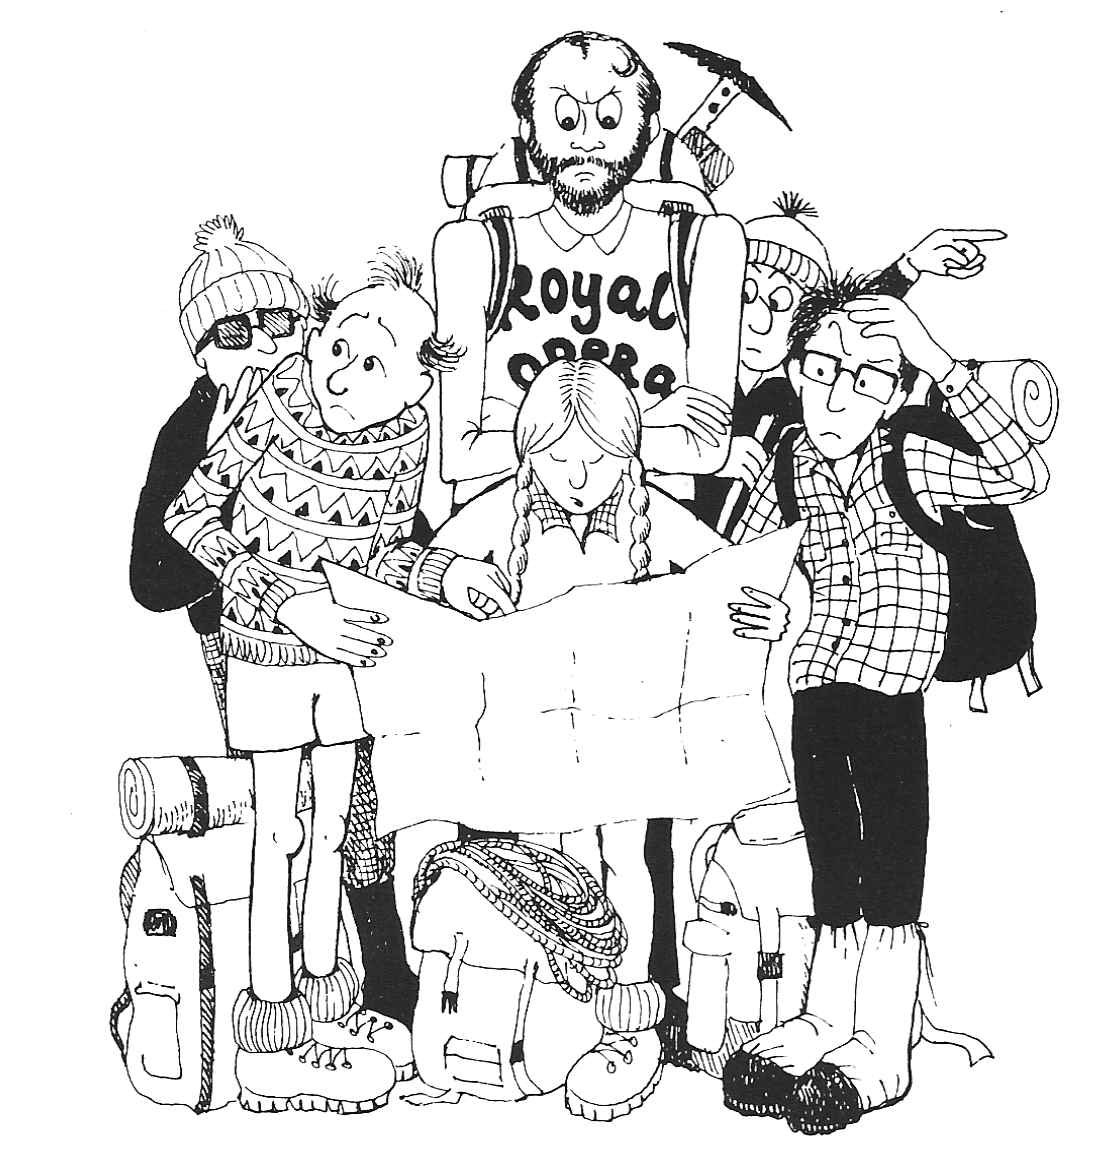
\includegraphics[width=.9\linewidth]{./images/Cartoon_11.jpg}
\caption{\label{fig:org37d0ada}
La Grande Epique}
\end{figure}

\begin{figure}[htb]
\centering
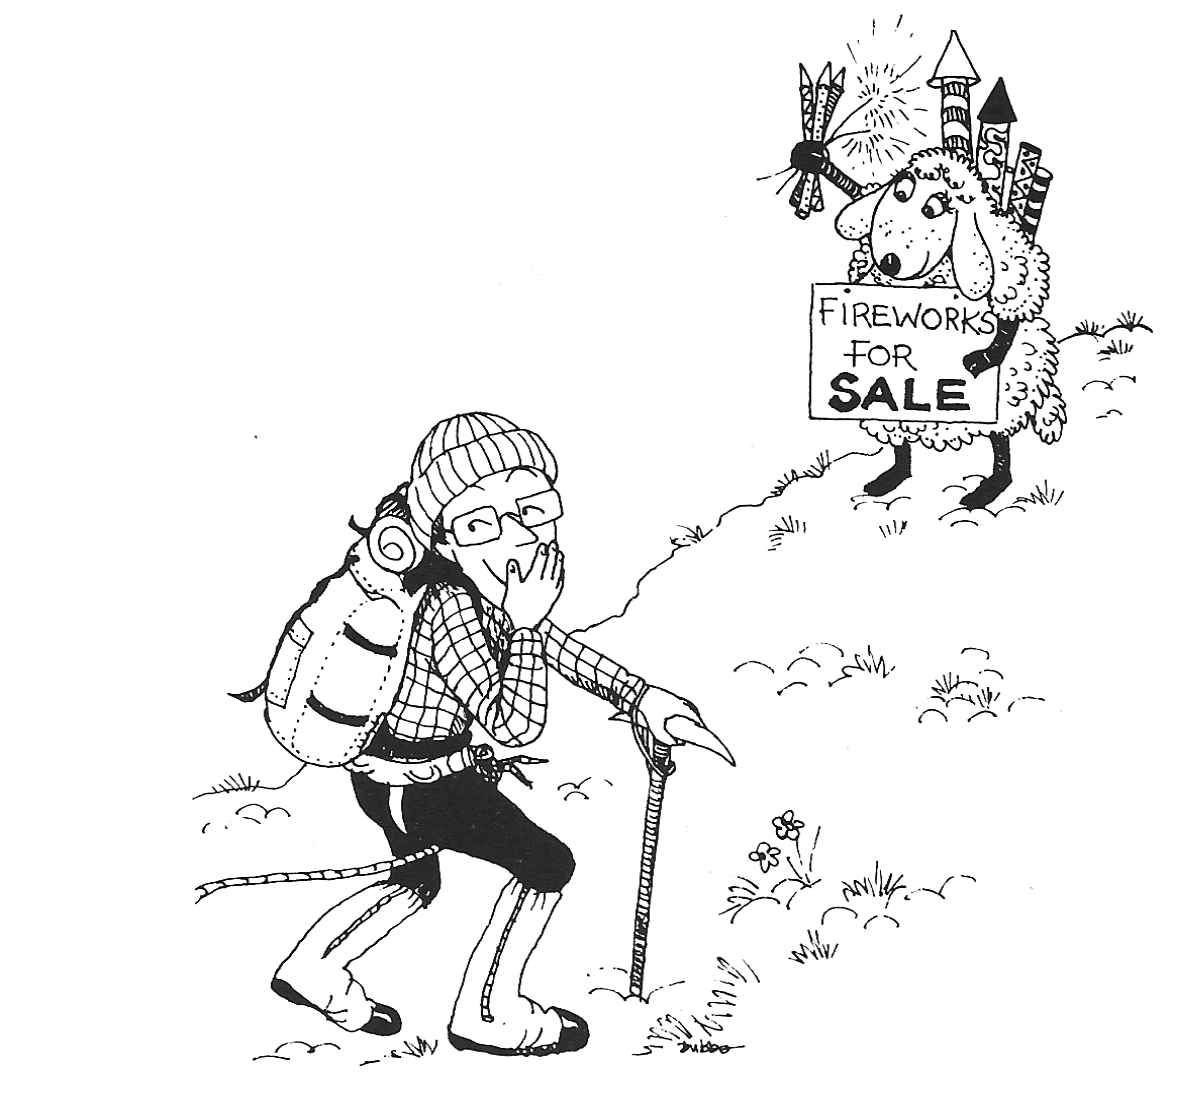
\includegraphics[width=.9\linewidth]{./images/Cartoon_12.jpg}
\caption{\label{fig:org98d04a4}
La Grande Epique}
\end{figure}

\begin{figure}[htb]
\centering
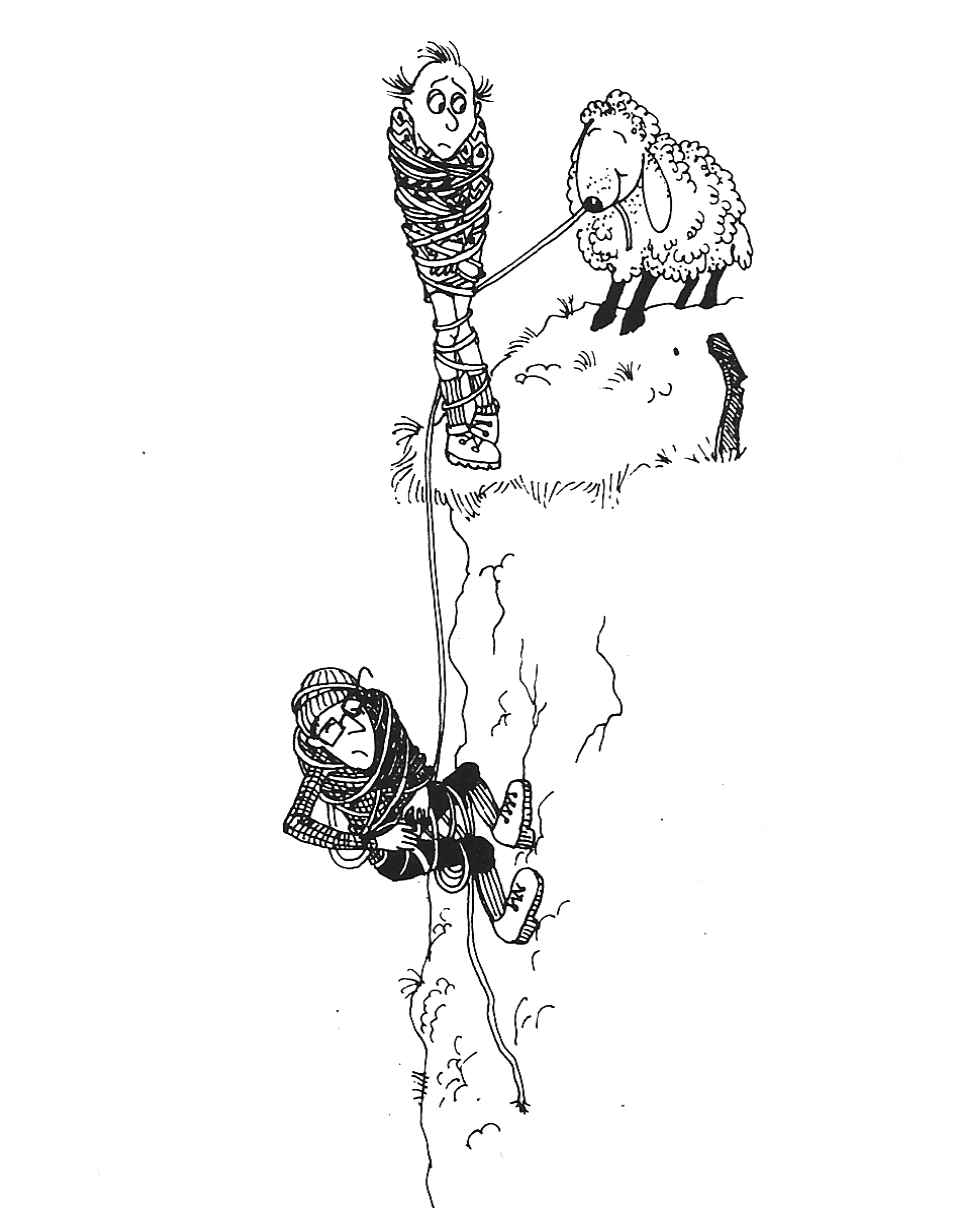
\includegraphics[width=.9\linewidth]{./images/Cartoon_13.jpg}
\caption{\label{fig:org1f20f47}
La Grande Epique}
\end{figure}

\begin{figure}[htb]
\centering
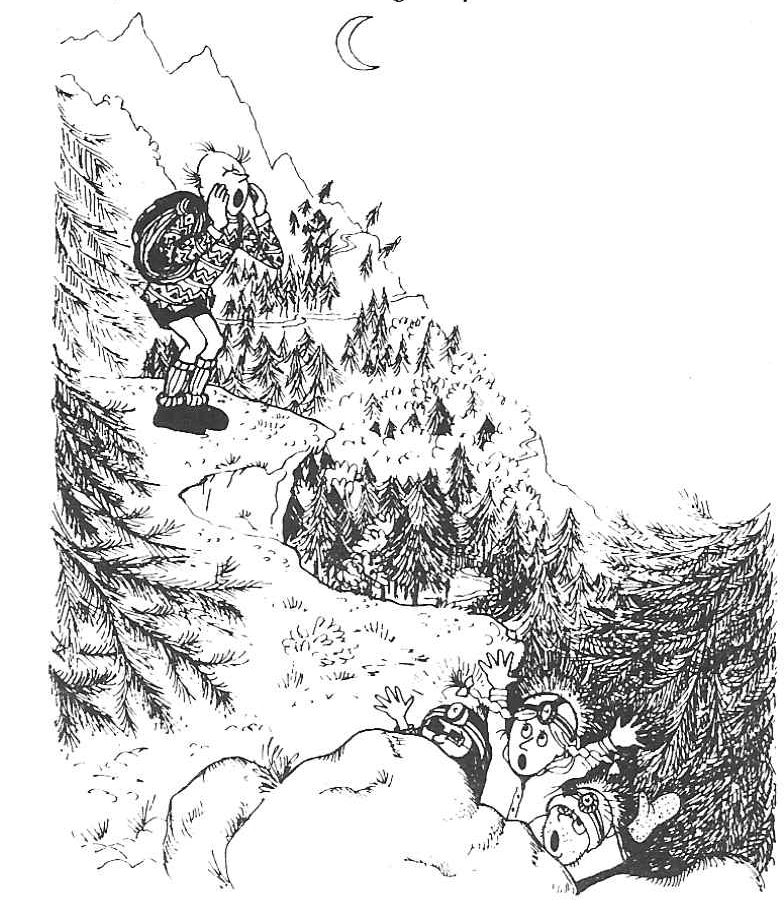
\includegraphics[width=.9\linewidth]{./images/Cartoon_14.jpg}
\caption{\label{fig:org9959041}
La Grande Epique}
\end{figure}

\begin{figure}[htb]
\centering
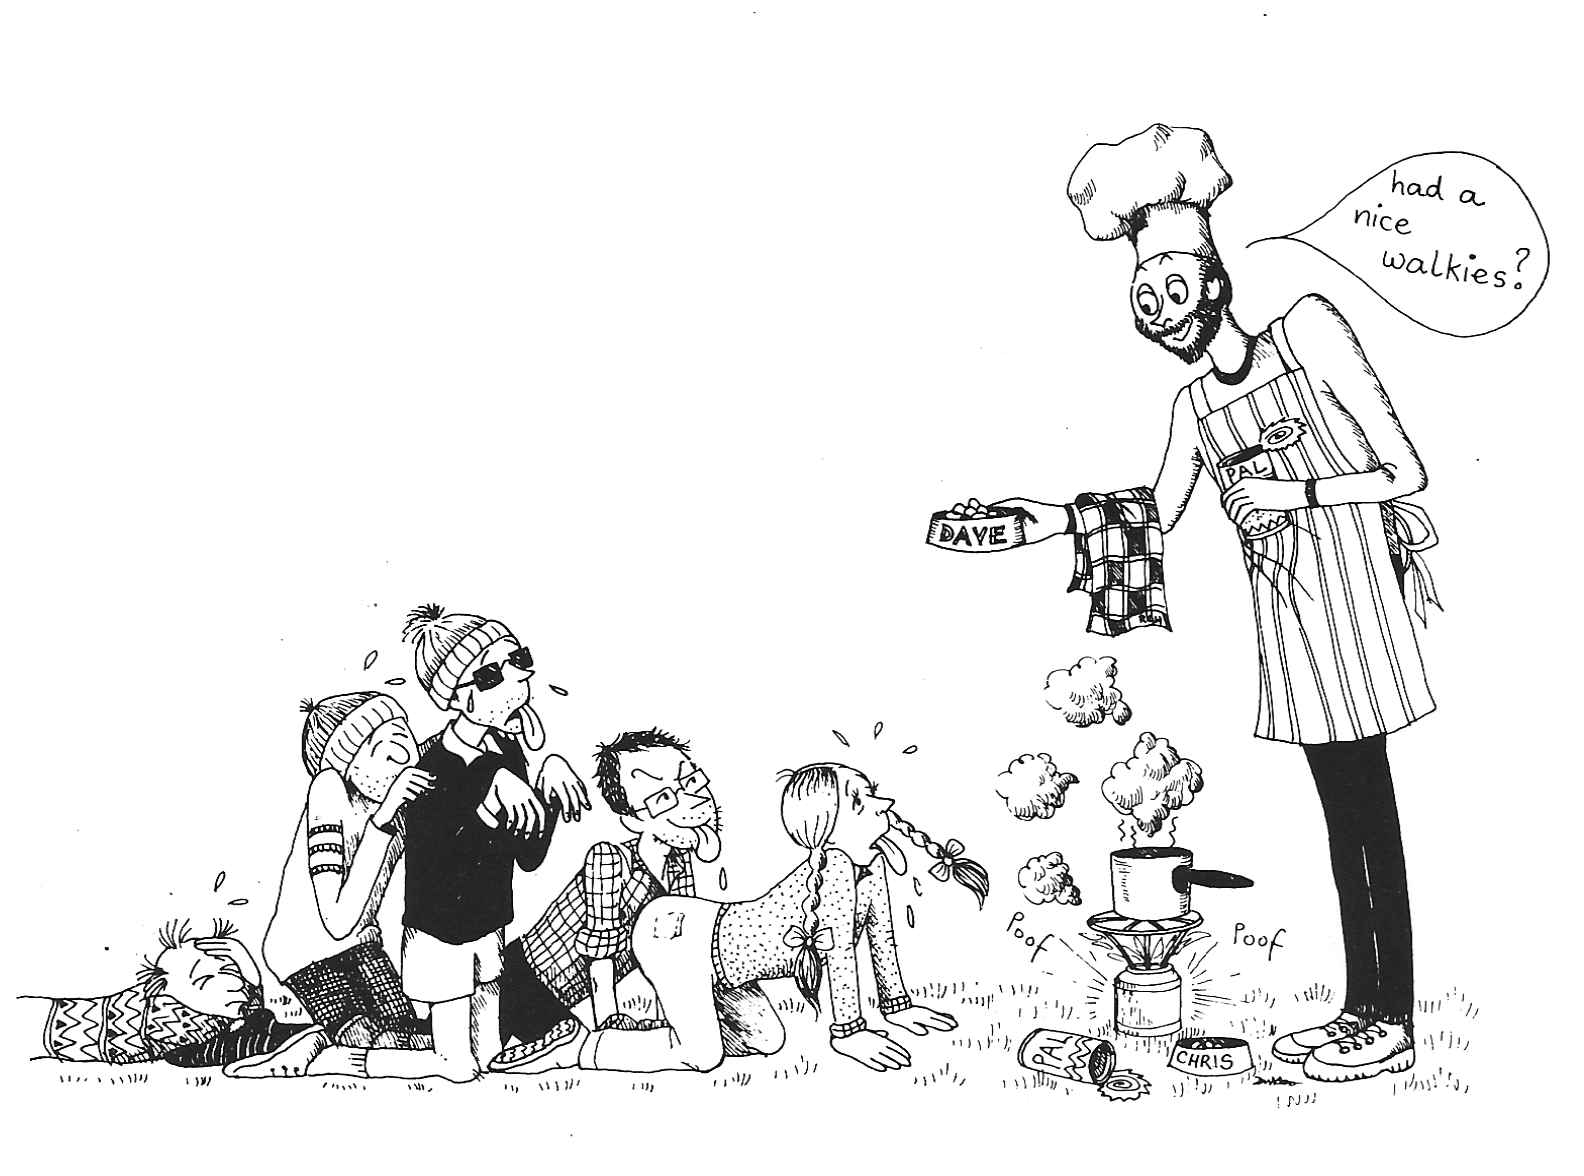
\includegraphics[width=.9\linewidth]{./images/Cartoon_15.jpg}
\caption{\label{fig:org2966bba}
La Grande Epique}
\end{figure}

\chapter{Route Major}
\label{sec:org03609e9}
\chapterauthor{Ian Barton}

The summer of 1986 was a good one in the Alps with a long
period of settled weather early in the season. I was camping at
Pierre d'Orthaz opposite the infamous Snell's Field. Unlike
Snell's, Pierre d'Orthaz has the advantage of being "legal" and
thus one's gear is not likely to be transported to the
Gendarmerie whilst one is away climbing a Route.

I had been in Chamonix for a few weeks so had already
climbed several Routes and was quite fit and well acclimatised. I
had always wanted to climb a Route on the Brenva Face of Mont
Blanc and the meteo was predicting at least two days of good
weather, so this seemed like a good time to try. The Brenva Face
is one of the largest and most impressive in the Alps. Situated
on the Italian side of Mont Blanc, framed between the Brenva
Ridge and Eckpfeiler Buttress, it over a mile long and the Face
itself is 5000 feet high. Since it faces directly into the
morning sun, an early start is essential to get above the seracs
which dominate the lower part of the Face and to escape the
avalanches which sweep this part of the Face during the day.

The Face was originally explored by T. Graham Brown with
various partners in the 1930's. During this period he climbed the
three Routes for which the Face is famous:  Route Major ,
 Sentinelle Rouge  and  The Pear . All three routes are impressive,
tackling the biggest face on the mountain and leading directly to
the summit. There are no great technical difficulties but all the
routes are exceptionally long, are at high altitude and there is
considerable objective danger from avalanches. I particularly
wanted to climb  Route Major  which takes the great snow ice
buttress defining the left hand side of the Great Couloir in the
centre of the Face.

I had arranged to tackle the climb with Gareth, a Scot, who
had climbed the  Brenva Ridge  a couple of weeks earlier with some
mutual friends. They had in fact been planning to climb  Route
Major  but after first getting lost trying to find the hut and
then failing to traverse far enough across the bottom of the Face
 a common mistake  they had ended up on the  Brenva Ridge . Near
the top of the Route one of the party who was not acclimatised
had then got into difficulties and it had taken them a very long
time to climb the final slopes leading to the summit of Mont
Blanc. Just below the summit they had also come across two other
Brits  who had climbed the  Cecchinel Nomine  route on the
Eckpfeiler Buttress. One of them was in a bad way, had collapsed
from exhaustion in the snow, and had to be helicoptered off   but
that is another story.

We decided that the best way to tackle the Route was to
travel light and climb quickly, moving together, in order to
minimise our exposure to objective dangers. We took only one nine
millimetre rope, two rock pegs and two ice screws but we had
plenty of food, most of which we ate at the hut before starting
the climb. I had no spare clothes and the only item in my
rucksack during the climb was a cagoule. The Route would be a
three day trip from Chamonix: an afternoon to reach the hut and
an overnight ascent  climbing the Face while it was frozen into
immobility , followed by a bivouac in the Vallot hut just below
the summit of Mont Blanc. The next day we would descend via the
ordinary route to Chamonix.

Just to gain access to the Brenva Face from Chamonix is
quite an expedition in itself. The first stage is to take a
telepherique to the summit of the Aiguille du Midi  easy on the
legs but hard on the wallet  and to descend into the Vallee
Blanche which is traversed to one of two huts, the Ghiglione or
the Fourche. Finding the huts is a problem in itself, since both
are situated on a ridge overlooking the Brenva Face and are very
difficult to locate from below. I had been to both previously but
I never knew which hut I was going to end up at until I actually
arrived there. Following tracks on the glacier, we climbed up a
steep icy gully to the crest of the ridge and finally arrived on
the balcony of the hut about six in the evening  it was the
Fourche.

The hut itself is very small, sleeping only eight to ten
people, but the view is outstanding since from the balcony the
whole of the Brenva Face is clearly visible. Leaving the hut
would be particularly exciting, an abseil from the balcony onto
the glacier below being necessary. It is definitely not a place
for sleepwalkers. From the hut our line of approach would cross
the upper part of the Brenva Glacier, climb over Col Moore and
then traverse the bottom of the face until below the large rock
tower, the  Sentinelle Rouge . Climbing up slopes of snow and ice
to the Sentinelle Rouge we would then traverse the Great Couloir
to reach the foot of the great rock ice buttress which forms the
substance of the route. All this section is very exposed to
avalanches and consequently must be completed at night. The
buttress provides the most difficult climbing but is safe from
objective danger and leads to the summit ridge between Mont Blanc
de Courmayeur and Mont Blanc.

The hut was full of Italians who were intending to climb the
 Brenva Ridge  with a guide and also two other Brits who were
planning to climb the  Frontier Ridge  on Mont Maudit. We managed
to squeeze into a corner near to the door next to a couple of
inscrutable Japanese and began to cook our food. This annoyed the
Italians who complained that the stove made too much noise and
was keeping them awake. Ignoring the protests, we carried on
cooking and filled ourselves with spaghetti and baked beans. Just
after we had finished and the Italians had returned to their
slumbers, a couple of Scots lads arrived and began to cook their
food, once again arousing the Italians' ire. We had a brief
conversation with the two Japanese and discovered that they also
planned to climb  Route Major  the next morning.

It proved impossible to rest in the crowded hut, so we
abandoned our plan of staying there until 2.00 am and left at
11.00 pm instead. Someone had kindly left a rope hanging from the
balcony of the hut but it was only after abseiling to the end of
it that we discovered that it stopped thirty metres short of the
glacier. Gareth was not impressed, but luckily it was too dark to
visualise the consequences of a slip. Some quite tricky climbing
down steep ice and chossy snow lead down to a final leap over the
bergschrund onto the glacier.

Roping up, we started to plod across the glacier towards Col
Moore. A nearly full moon illuminated our progress in the icy
cold of the night and we congratulated ourselves on our good
fortune. However, a few minutes later, and as if to spite us, the
moon disappeared behind the summit of the Blanc and everything
suddenly went dark. Switching on our head torches we carried on
over the Col and began to traverse below the Face across the
avalanche prone gullies. Huge blocks of ice littered the glacier,
evidence of the avalanches that fall here during the day. At this
point Gareth's head torch went out and we had to stop and take it
to bits  not easy with freezing hands and in the dark  but could
find nothing wrong. We re assembled it and as if by magic it
started to work again. Looking back towards the hut we could see
the two head torches of the Japanese as they began their descent
onto the glacier.

Gareth was determined not to repeat his previous mistake and
we continued for what seemed like miles across the bottom of the
Face until, above us, we could see what appeared to be the  Red
Tower . Crossing the bergschrund in order to get established on
the Face proved tricky, as the upper lip was covered in
unconsolidated icing sugar. Burying my axes in the snow up to my
armpits I managed to mantleshelf and did a belly flop onto the
slope above.

Shortly beyond the bergschrund the icing sugar changed to
hard ice and we were funnelled into a wide gully. Rounding a
corner we found ourselves below some small seracs, but avoided
these by climbing a small ice ramp which split them. The gully
then became wider and we could see at an indeterminate distance
higher up what we assumed to be the  Sentinelle Rouge . The
climbing was quite tiring because of the hard and polished
surface of the ice. Small chips of ice slithered down the slope
towards us and below we could see vast piles of avalanche debris
at the bottom of the Face.

After climbing some distance up the slope it became obvious
that what we had thought, in our ignorance, to be rocks
sheltering us from possible avalanches were in fact more seracs,
this time much bigger and highly dangerous. The little slivers of
falling ice now assumed a greater significance as we anticipated
the really big fall which would sweep us from the slope. We were
now clearly lost but had no alternative but to continue and we
soon reached the seracs. Luckily we found an easy line, climbing
them by one long but quite steep pitch.

Thinking that the danger was now past, our illusion was
shattered as above us we could see yet a third and even larger
row of seracs. After climbing over some smaller formations we
arrived at the base of the main barrier. It was my lead and I was
distinctly worried as I began to work my way up the steep ice.
The climbing was very steep and the ice hard and dinner plating.
I had no way of knowing if I would be able to reach less steep
ground and a belay. Fortunately, I reached the top of the serac
with about twenty feet of spare rope. Seconding this pitch was
just as nerve racking for Gareth as the belay was a single ice
screw and so the rope offered only an illusion of security.

Once we had surmounted the last serac we could see a rocky
ridge up to our left and decided to make for this, thinking that
we would be safe on its crest. The slope seemed to go on for ever
as, acutely conscious of the need for speed, we climbed towards
the rocks. Eventually we reached the foot of the ridge and found
an easy gully leading to its crest. Safe at last, we paused for a
good look around. Suddenly everything clicked into place as I
could see the  Brenva Ridge  far below us. We had climbed the
couloir and seracs to the right of  Route Major  and were now above
all the difficulties and out of danger.

Far below us we could see the head torches belonging to the
parties beginning their ascent of the  Brenva Ridge . It was two
o'clock in the morning and we had managed to climb 4000 feet of
difficult ground: far from being slow as we had thought, we had
in fact been climbing extremely fast!

Gareth was very annoyed at having missed his chosen Route
twice in succession and we sat down to discuss what to do next. I
was equally annoyed about having got lost, but was even more
relieved that we were finally off the Face. However, it was still
quite a way to the summit up a long and tedious snow slope which
we both knew would be hard going at this altitude. Disillusioned
at having failed to find the correct line, we had the alternative
of descending the  Brenva Ridge  back to the hut, enabling us to
return to the fleshpots of Chamonix that afternoon. This route
would at least be sheltered from avalanches if the sun hit the
Face before we had completed the descent.

The decision to go down was duly made and we lost height
rapidly. Close to the bottom of the ridge I suggested descending
a gully on one flank to save time instead of going all the way to
the end of the ridge. However, at the foot of the gully we could
not discover any way over the bergschrund and we were forced to
traverse along the base of the  Brenva Ridge  to a point where the
bergschrund narrowed. This lead us directly beneath the seracs
overlooking the Gussfeldt Couloir! After jumping the bergschrund,
we ran down the slope below and out of the fall line to safety.

Plodding back across the glacier we were treated to a
magnificent sunrise over Mont Maudit but to complete our
catalogue of errors we managed to end up at the Ghiglione hut.
Shortly after our arrival there was a tremendous noise and on
rushing outside we saw a massive avalanche from  The Pear  seracs
sweeping the route we had been climbing. We retired to bed,
suitably chastened, for a well earned sleep. Later in the day, as
we left the hut to go back down to Chamonix, I had a good look at
the Brenva Face and saw that whilst we had been sleeping there
had been another avalanche, this time from the seracs above the
Gussfeldt Couloir below which we had traversed on our descent.

The walk back up the Vallee Blanche proved extremely tiring
and we only just caught the last telepherique down to Chamonix.
When we got back to Pierre d'Orthaz the lads told us that two
people had been killed on  Route Major  the previous night and they
had thought it must have been us. Luckily we had got back before
they had sold our gear!

The next day we wandered into the Guides Bureau and looked
at the Definitive Routes Book. It seemed that no one had
previously climbed our line so it would appear that we had done a
new route by mistake, although I doubt if anyone will wish to
repeat it. We asked about the two people who had been killed. A
Guide told us that two Japanese had been overwhelmed near the
great Buttress by an avalanche. This had happened at just about
the time we should have been climbing the Buttress had we left
the hut when we had originally planned.
\begin{figure}[htb]
\centering
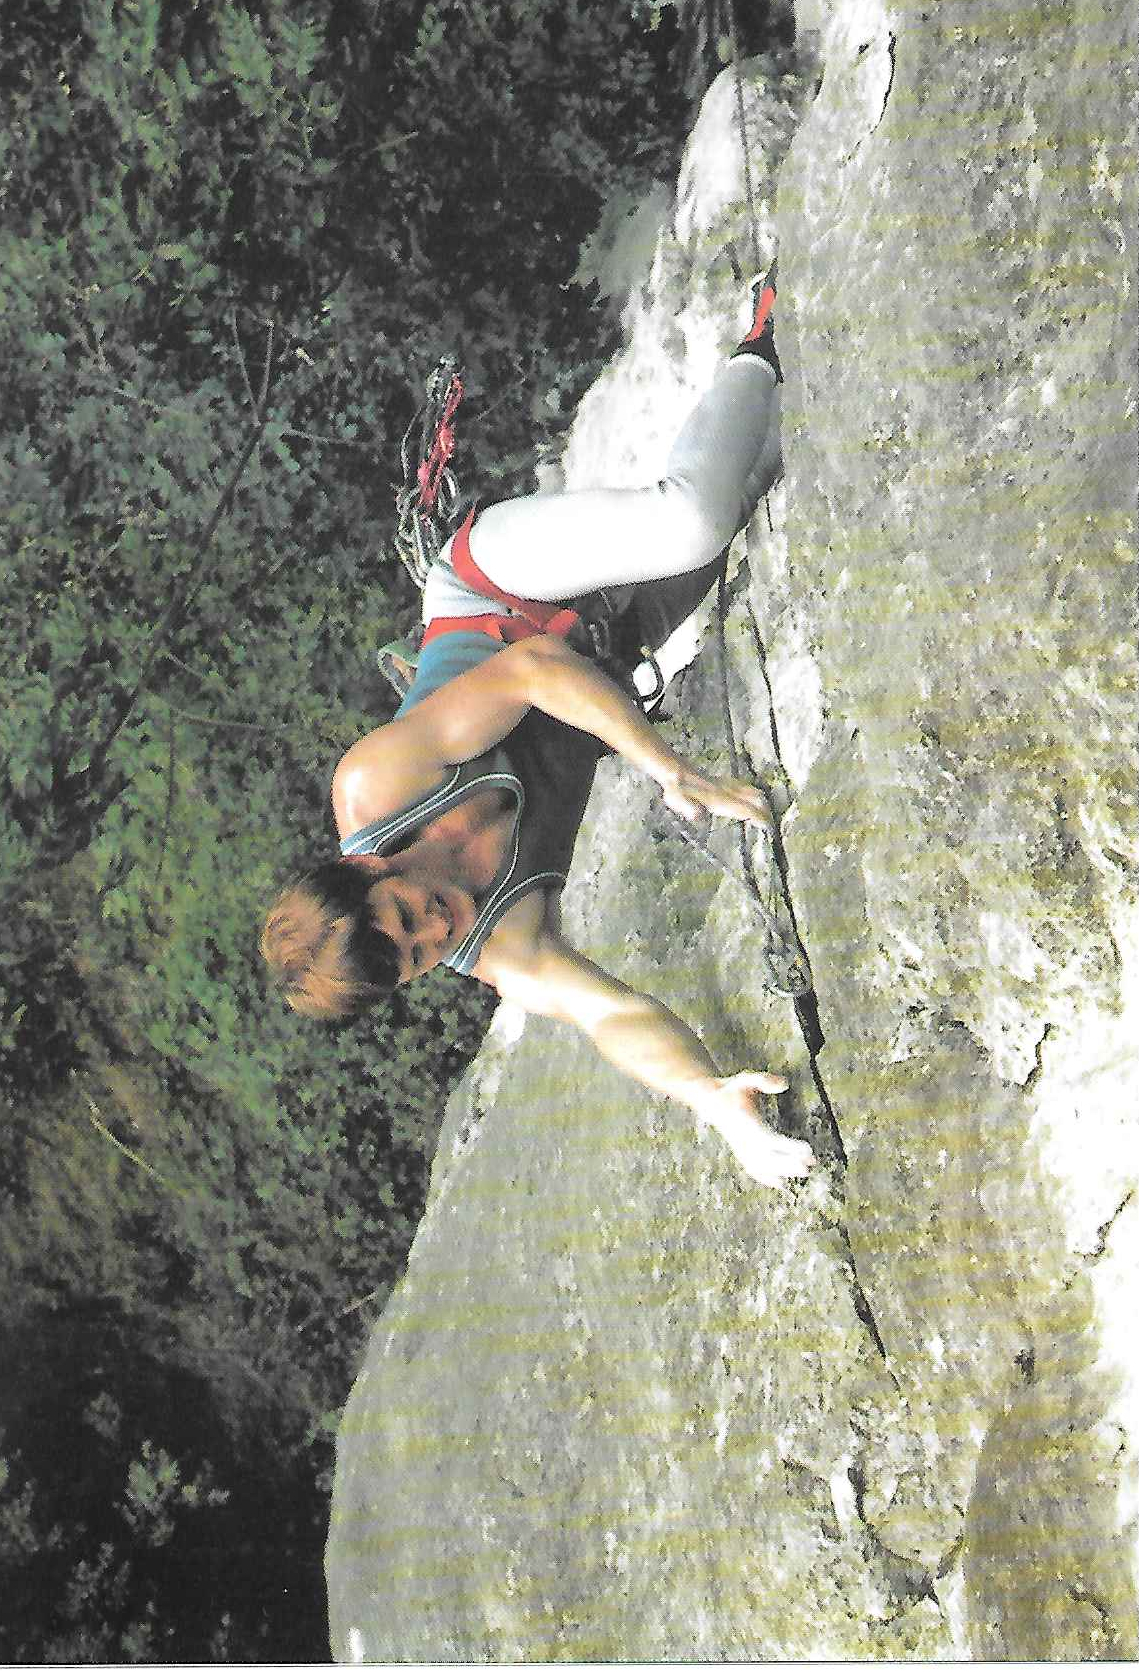
\includegraphics[width=.9\linewidth]{./images/Chris_Wright_at_Water_cum_Jolley.jpg}
\caption{\label{fig:orga9b65b6}
Chris Wright at Water cum Jolley}
\end{figure}

\chapter{From Toothbrush to Sledgehammer}
\label{sec:org5afd1f5}
\chapterauthor{Steve France}

The winter of 1985 86 was The Castle Mountaineering Club's
biggest climbing triumph - yet not many members know the true
extent of the Club's success. More new routes were claimed on one
crag than probably all The Castle's other first ascents put
together.

The "secret" Quarry is situated on the right as you travel
up the road from Stoney Middleton and is accessed via a gate and
track which leads to the quarry base. The main wall, which is
almost vertical, extends some hundred feet in height to a huge
ledge which effectively splits the face, forming an upper tier of
fifty feet.

When Steve France, Chris Wright and Ian French entered
Horseshoe Quarry for the first time, the true potential of the
place was finally realised. Its loose and dangerous condition was
enough to put anyone off, but what was required was a bit of
vision and imagination and between the three of them there was
certainly that. The Big Question was, would they be wasting their
time developing an area which nobody would bother to visit? Only
time would tell, but the first thing to do was to clean the place
up and to make it worth climbing on. It didn't take long to
realise that any glory to be had would not come cheaply.

At first the usual gardening equipment was used -  wire
brush, toothbrush, small trowel and broddling stick   but it
didn't take long to realise that these tools were totally
inadequate. Steve had started to clean a small ledge on his first
new route and after shovelling at least half a ton of rubble
discovered he no longer had a small ledge but a huge belay stance
for about a dozen people. Furthermore, the bigger the ledge got,
the shorter the route became, as he slowly filled up the quarry
bottom with its debris. Steve later became known as the Mad
Axeman due to his mean short pick-axe which he used for levering
off small flakes, boulders, in fact anything that moved  or
didn't   but that is another story .

In the early days of development, huge amounts of rubble and
rock were detached in order to clean up the cliff face. This was
not just confined to the routes themselves but the rock was
generally cleared all over in a desperate attempt to make the
place safe and more appealing: apart from that, "spoffing" blocks
happens to be bloody good fun. The biggest trundle was a gigantic
hanging pinnacle weighing at least five tons, situated half way
up the wall on the left hand side and poised ready to fall at any
time. The Mad Axeman picked away at its footing like a
masochistic dentist but alas failed in the attempt. The next day,
not to be outdone, the giant tooth was attacked again but this
time with a large pick and a six foot long crowbar. The resulting
"bavoooooom" must have been heard for miles. Well worth the
effort!

The most controversial decision was the use of bolt
protection . Due to an instinctive desire to live, bolts were
necessary having regard to the quarry's lack of natural fault
lines, which meant that there were few  if any runner
placements. Even pegs were bottoming after only an inch of
penetration. Sounds painful! By strategic placing, it was in fact
possible to use only four bolts to protect a hundred feet of
climbing  these were pre-placed during the last stage of the
cleaning operation.

The actual leading of the routes was  in accordance with
modern day ethics  done without practice or top rope - to make
the ascent as pure as possible.  Even this was not pure enough
for Steve Ralph who at a later stage amazed us all with his
"clean lead on sight" policy.

Developing the upper tier also had its problems due to the
lack of abseil points at the top.  So Chris and Steve had to
sledge hammer a series of belay stakes into the ground each day
these they buried under piles of stones to prevent others from
using them until the routes had been claimed. The top was very
reminiscent of Millstone with its loose shale and grovelling
finishes and so platforms were dug out of the sloping earth to
enable everyone to actually finish the route instead of wondering
if the protection was good while free falling! This also had a
second advantage in that it prevented a constant dustfall down
the rock face, previously inevitable whenever the wind blew.

As with the main face, there was plenty of loose rock to
detach on the top tier. Unfortunately it had a tendency to roll
over the lip of the main ledge and go crashing down the main wall
below. Although this was two for the price of one, everyone had
to know where everyone else was and anyone who decided to go
walkabout did so at his own risk.

By the time of the New Year, Ian had finished four of the main
lines on the lower wall, including  Megalithic Man  and  Ancient
Rhythm . Steve had completed his excavation of the ledge and named
the ensuing route  Nice Face, Shame About the Ledge . Chris, who by
now had the misfortune to be working for a living, had half cleaned
a route on the lower face but then decided to join Steve
with the Upper Tier development with his eyes set on Mr Blue
Sky .

However, all good things must come to an end and the word
was finally out, bringing visitors to the quarry. The self indulgence
of eating the cherry cake might have to be shared!

The fun now began in earnest because many routes had been
cleaned but not led - including the one Chris had started
cleaning earlier and this was the route which another group was
eyeing up first! There was no time to lose but Chris was at work
and not available until the weekend, so the honours went to Steve
who climbed the route and called it   Shot Yer Bolt . Not
surprisingly, Chris was displeased, so Steve gave him one of his
unclimbed cleaned routes as a peace offering - subsequently named
 White Dove . During the next few weeks a spate of ascents were
made and the pressure to complete new routes was reduced.

Ian Barton and Steve Ralph now entered the quarry with the
promise from the trio that there were new routes to be had,
especially at the lower end of the gradings. Ian wasn't impressed
but made a token gesture of several rock routes and an ice gully
at the back of the quarry. Unfortunately  or fortunately!  only
one of Ian's routes were attributed to him in the guide book and
Steve Ralph received the honours instead.  In fact Steve R. was
"given" quite a few routes he knew nothing about, due less to the
generosity of the new ascentionists but more to their
embarrassment in owning up to them! This may be unfair to Steve
R., but perhaps due to the loose, dirty, and dangerous routes
which he led, he asked for it!

There is a true report of a pair of French girls who
recently visited the quarry, and after no success in climbing the
higher grades, were kindly directed towards the   Bimbo \ldots{}
routes. After struggling and cleaning for an hour and a half they
finally screamed "Quelle Masse de Garbage" and walked away
feeling totally disillusioned with British Climbing.

After four months of digging, the novelty finally wore off
and the very sight of a wire brush or shovel prompted a baulk of
revulsion. Altogether, thirty five routes were climbed by The
Castle with sixteen of them being attributed to Steve Ralph.  As
for the original trio, they all succeeded in their secret desire
to bag their first 6b virgin ascent. With all the best lines
gone, The Castle left the quarry to the droves of scavengers that
poured into it. The potential for new routes was still as strong
as ever, although much of the remaining surface contained loose
rubbish. It was nice to see the interest that the quarry provoked
but in the long term it will probably suffer from enthusiastic
young leaders willing to climb anything, however loose, for the
sake of immortality.

On visiting the quarry today you will usually find several
parties climbing there. The original vision of Ian, Steve and
Chris has finally reaped its reward. The rock dries exceptionally
quickly and, coupled with the bolt protection, makes it an ideal
crag for the winter or wet. Unfortunately the routes at the lower
end of the scale tend to reflect the nick name Horseshit Quarry
but if you do routes of 5b or harder you may well be very
pleasantly surprised, although probably knackered as well.

\chapter{Western Gully, Black Ladders}
\label{sec:org45870fd}
\chapterauthor{Ian Barton}

"This is going to be a straightforward climb with no epics
or benightments. I've done the route before, it's grade IV and we
are going to make a really early start, so there is no chance of
getting benighted." Knowing grins were exchanged by the others.

The route in question was  Western Gully  in North Wales. The
climb is on a crag called  The Black Ladders  Ysgolion Duon  in
the heart of the Carneddau. Next morning I kept my resolution
about making an early start and we were away from the hut by
5.00 am. I also had a very strong partner in the form of Caveman
 Andy  so success and descent before the pubs closed seemed
assured, as we drove round to Bethesda and began the long walk up
Cwm Llafar.

The first setback occurred when we arrived at the bottom of
the gully at about 7.00 am to find that everyone else had also
got up early. I suppose the route's inclusion in "Cold Climbs"
accounts for its popularity, as people add it to their tick
lists. Two parties were already established on the first pitch
with numerous others waiting their turn at the bottom and we
could hear sounds of others higher up the gulley. Andy and I
geared up surreptitiously to one side of the crowd and when we
were ready, played our trump card. Cheating outrageously, Andy
led up the steep frozen turf to the left of the first ice pitch.
The crowd fell silent and stared at us, amazed that we should
manage to outflank them by this simple manoeuvre. Andy reached
the first stance having successfully overtaken two parties and I
climbed quickly to reach him. We were now near the front of the
queue and, moving together on the easier section that followed,
we overtook all but one pair.

Catching up with the two at the front of the queue just
below a steep section, I belayed and brought Andy up to me. The
pair in front of us had managed to get their ropes into a bit of
a tangle so we had to wait while they sorted things out. Looking
up at the continuation of the gully there was hardly any build up
of ice, with only a veneer of verglas and a dusting of powder
snow covering the rocks. Eventually the way was clear and Andy
set off up the next pitch. This was a narrow chimney with an
awkward exit at its top. Climbing in his usual fast and efficient
style he had soon reached the next stance, making it all look
easy. When it was my turn to follow I found the ground anything
but straightforward and struggled to get out of the chimney.

The team in front of us were now at grips with the famous
chockstone pitch. The leader had inserted a peg upside down in
the roof and was busily knocking all the ice off the steep wall
which is the key to avoiding the overhang formed by the
chockstone. Eventually he overcame the chockstone but took even
longer to get up the remainder of the pitch while we waited our
turn in the icy cold of the cave under the chockstone. At last he
was belayed but his second struggled on the first section out of
the cave, demolishing the remaining ice before disappearing into
the chimney above. Eventually it was my turn. I climbed easily up
to the peg but several attempts to climb the wall to one side of
the chockstone were repulsed by the lack of ice and resulted in
clattering descents to the floor of the cave. Finally I managed
to fix a wire in the roof of the cave and using this for aid, I
reached over the chockstone. Jamming my axes in the crack above
the chockstone, I heaved myself up around it.

I was now in a very precarious position in a narrow chimney,
but a few feet above me it widened and after a few rapid bridging
moves I was able to wedge myself securely. It was only then that
I noticed a peg below my feet just above the chockstone and which
I had failed to see in my previous haste. There was no prospect
of other runners nearby so I reversed the previous delicate moves
and reached down, managing to clip into the peg at full stretch.
Regaining my wedged position, I contemplated the ground above.
The narrow chimney continued with just a glaze of ice on the
walls, enough to make normal rock climbing impossible but not
enough to allow for the use of Chacals and crampons. I did not
fancy tackling any of this without some more runners but the only
obvious crack was too small to take my one channel peg. After I
had relayed my feelings about the lack of runners to Andy, he
asked two women who had just arrived in the cave if we could
borrow one of their pegs. While the peg was being sent up to me I
overheard a snatch of Andy's conversation with them.

"Do you know Dai Lampard then?"
"Yes, quite well, he's my husband!"

Even their smallest peg proved to be too big and eventually
I threaded a sling around a thin icicle, convincing myself that
it would hold my weight if I fell. However, there was now another
problem: the chimney was too constricted to climb with a sack.
Further contortions enabled me to remove the sack and hang it
from the icicle. As I struggled to climb above the sack, the ice
shattered and all four points of contact parted company from the
ice at once. I began to  slither down the chimney, the icicle
thread broke as my weight came onto it and I was heading down
over the chockstone onto the boulders underneath. Luckily, with
my Chacal I managed to hook the crab clipped into the peg above
the chockstone. This arrested my fall but I was now tangled up in
the ropes and the sack.  After tussling for a few minutes with
the tangle of gear while hanging on with one arm, I managed to
get sorted out and was once again safely wedged in the chimney.

A further session of digging out likely looking cracks
resulted in a hex hammered into the back of the chimney. I now
hung the sack from this and set off again up the chimney. This
time I was more careful with the ice and reached a better thread
round an icicle about twenty feet higher up. Above this the
difficulties eased slightly, the ice got thicker and I was able
to rest. At the top of the chimney there was an awkward move out
onto a slab but a hairline crack provided a good placement for a
knife blade. There was one final small bulge and I was then in a
second cave with massive spike belays to which I thankfully
lashed myself.

Looking back down the gully as I took in the rope and
started to bring Andy up, I could see that all the other parties
had given up and were abseiling off. Andy climbed whilst I
alternately took in one rope with the sacks attached and then the
other rope with Andy on it.
	"You had better get your head torch out" he said as he
arrived, "It'll be dark soon."
	Looking at my watch I saw it was nearly four o'clock! We had
been on the route for over nine hours although it had seemed far
less.

The next pitch was quite short, up a slab onto easier ground
above. In good conditions the slab is covered in ice but, on this
occasion it was just dusted with powder snow. Andy balanced up to
a peg, crampons scraping on the rock and then mantleshelved onto
the peg. A few more delicate moves above this and the climbing
was easier. When my turn came to follow I was impressed with his
efforts as I found the climbing very insecure and was glad that I
hadn't had to lead it. By this time I was completely knackered so
Andy offered to lead on. The next pitch was straightforward with
only one awkward boulder to surmount. Above this the climbing
became easier and we moved together on the upper section of the
gully to the top.

As I emerged Andy walked forward and shook my hand  it had
been a great climb.

It was a starlit night with perfect visibility.
	"There should be no problem getting off. All we have to do
is to follow the rim of the cwm round keeping it on our left and
then go down the easy slope to the bottom of the crag," I said.

We set off, keeping close to the edge so as not to lose the
way. After some time I was convinced that we had reached the
point at which we should descend into the cwm. However, I had
nagging doubts   there were lights in the valley below, where
there had no right to be any and the steep descent that I
remembered was an easy angled slope. We kept on going, eventually
reaching the bottom, but it did not look anything like Cwm
Llafar. After walking down the cwm for some time Andy shouted
that he had found a tarmaced track. Suddenly I knew where we
where. We had descended into the Ogwen valley and the lights in
front of us were in fact those of the hut!

Soon we reached the hut and walked in to hoots of derision.
This was the second week in a row that I had descended in the
dark and walked off the wrong side of the hill!

\chapter{Prince Charlie's Castle Tramp}
\label{sec:org46df898}
\chapterauthor{Dave Kime}

The idea was dreamed up in Culra Bothy on a dark November
night. The parents-in-law were in New Zealand and had taken to
backpacking and bothying. Soon they were to retire, so what
better than a short backpacking trip for them around the Scottish
Highlands? What evolved was a 200 mile trek through the glens,
linked with some stretches of imagination to the stravaigings of
Bonnie Prince Charlie. There was perhaps even more of a link with
the wanderings of the CMC and these came to mind from time to
time as we acted as support party for the walk.

The Tramp started at the Prince's Cairn on Loch nan Uamh
whence it is but a short sail to the Isles. The Cuillin of Rhum,
visible from the hills between here and Lochailort Hotel, brought
to mind the climbs and scrambles on that ridge, of nights in
Dibidil Bothy, of bivvies on Allival watching the sunset and the
flying bunnies returning to their nests after a day's fishing
and of a descent from Orval in thick cloud down a steep gully
with Andy and myself leading only ten feet apart and our
compasses pointing in opposite directions. The Tramp continued
now across wild country to Oban Bothy on Morar where the
isolation became apparent when a maternal shoulder was dislocated
crossing a swollen burn and we evacuated by Glen Pean.

The Bothy here was now deserted, unlike our visit late one
December when our sleep had then been disturbed at 3 am. Morning
revealed two bodies upstairs and two crates of whisky downstairs
and by evening, crowds were appearing through the blizzard from
all directions and the wall was stacked high with whisky, beer,
turkeys and more. St. Andrews University MC were celebrating New
Year here in true Scottish style, including a midnight swim in
the burn by the President  who'll suggest at the next AGM that we
adopt this tradition?  Undeterred, we started to cook the curry
in a quiet corner, until a snowman appeared and asked if there
was anyone from Sheffield with a ginger beard. Our friends had
gone to A'Chuill Bothy, he informed us. A moonlit walk with a
half-cooked curry took us in a few miles to this darkened Bothy
where at 8 pm we awoke Andy and Rosy and two strangers, lit some
candles and continued cooking the meal. Mice  rats?  nibbled at
the left overs while we slept.

We passed above A'Chuill again the following year as we
continued the next stage of the Tramp, across to Kinbreak Bothy
and then to a camp in Glen Loyne where the river rose three feet
in the night. Decadence and the Cluanie Inn. Cluanie, land of the
Five Sisters, the Seven Brothers, the Three Uncles, the Two
Grannies and the South Cluanie Ridge, where in years gone by Rosy
had drunk a stream dry and Drew had tested a home made tent
almost to destruction.

The route now took us on through Glen Affric, where we had
once spent an Easter of hot sun and melting snow and saw no-one
for a week, and where we ticked off  Bens Chrysanthemum and
Sod-All  where the Youth Hostel was left open and unlocked and
was inaccessible by car. On to Fort Augustus and Loch Ness with
not a tick in sight and then the General's Road over the
Corrieyairack Pass where mother in law broke a foot in steep snow
and hopped three miles to the camp at Melgarve. Blue skies now
over Creag Meagaidh, where a decade ago we had walked in a circle
in a blizzard while the rest of the Club played hide-and-seek on
Carn Mor Dearg, tempted by Mike's slides of perfect weather on
the previous year's Glen Roy meet.

The Tramp continued again the next year, but after two
mishaps I left Jenny to act as support on her own. For
mother-in-law to be injured once might be a misfortune, twice
might be carelessness, but three times\ldots{}!  And so past  Garva
Bridge from which we had skied up the Monadhliaths, but now on to
Pattack and Culra Bothies. No time to call at Ben Alder Cottage
where the Club had kept the evil spirits at bay by liberal use of
the more benign malted type. Loch Ossian and its rail access
hostel, Loch Treig and on to Meanach Bothy.  Fourteen years
previously, we had used it before the Mountain Bothies
Association had fitted windows and doors. Straw beds and clear
skies with a million stars through the open window at night,
sun, snow  and ice on the Grey Coires by day.

Beyond were the Aonachs and memories of setting off one
clear October day from Glen Roy, stoked by egg and  bacon served
in bed in a frozen tent at 6 am, Al and  Kate ahead driving
erratically as they spotted birds at dawn  and from the summit,
distant views of all the Highlands. Cool enough for us but still
too hot for Jimmy to put a shirt on. Back in Sheffield two days
later, Mike's tent was still frozen, but his throat was still hot
from the vindaloo curry and gluwein which I had served at the end
of the previous day. The Tramp took us on past Binneins Mor and
Beag and the lochan between where the Club  once swam one wet day
in July. So on to Mamore Lodge, a friendly place for mountain
folk - what a change from  many years ago when an innocent new
member took up an offer to join Mike Munrotic for a walk in the
Mamores. The alarm went at 6 am when Mike's ample rear end hit
the floor at Lagangarbh  after a direct descent from the top
bunk. At 7.30 we drove up the private road past the Lodge and
were soon afterwards on the first Top, Am Bodach. By eleven the
Gearanachs \& Garbhanachs were done, three more ticks, and there
was just "that little conical job over there" to do to complete
Section Four. No messing about over Na Gruagaichean and Binnein
Mor for Mike: the direct route by a three mile traverse across
the rough heathery coire to Binnein Beag, but rewarded by the
sight of red deer in their thousands . Last tick of the Section
and back to the car. Two flat tyres but Good Scout Mike was
prepared with a hand pump and we were off towards the Lodge.

"Daddy, Daddy, they're coming!"

There followed a short legal discussion on the law of
trespass in Scotland from my solicitor to the local keeper whose
response sounded remarkably like "Bugger Off". The welcome is now
of a better type, but with all rooms taken we camped by the pond
and ate and drank in the bar. The tourist route of the West
Highland Way passes here and we followed it now before leaving
the ant-trail to cross to Corran ferry.

Across in Ardgour, Glen Scaddle led to Resourie Bothy where
one Christmas the two of us collected so much wood in just an
hour that we spent the whole evening trying in vain to burn it
all. Beyond is Ben Resipol where one New Year a Castle group
inched on their stomachs towards the summit, precariously
anchored by their axes in a blizzard with ferocious winds. We
failed and evacuated by the nearest gully which led to the bogs
by Loch Shiel. Next day the tabloids screamed "Gales Lash
Britain" and a neighbour later said:

"Yes, it was a bit windy, our dustbin lid blew off."

Warned of the bogs, the two pensioners completed the Tramp
by first rowing six miles down Loch Shiel to the new Hothersall
Bothy at Langal for the night  and then another two to Acharacle
before the path to their final bothy at Druimnich, where a number
of the Club have been conned into transporting large chunks of
oak and birch, seemingly for miles across hills and bogs, to keep
the winter fires burning.

When there's nothing left to tick and the last table of the
Scottish hundred footers has been put away, you can always invent
a walk though the glens to see you into your Seventies. Castle
memories await you there.
\begin{figure}[htb]
\centering
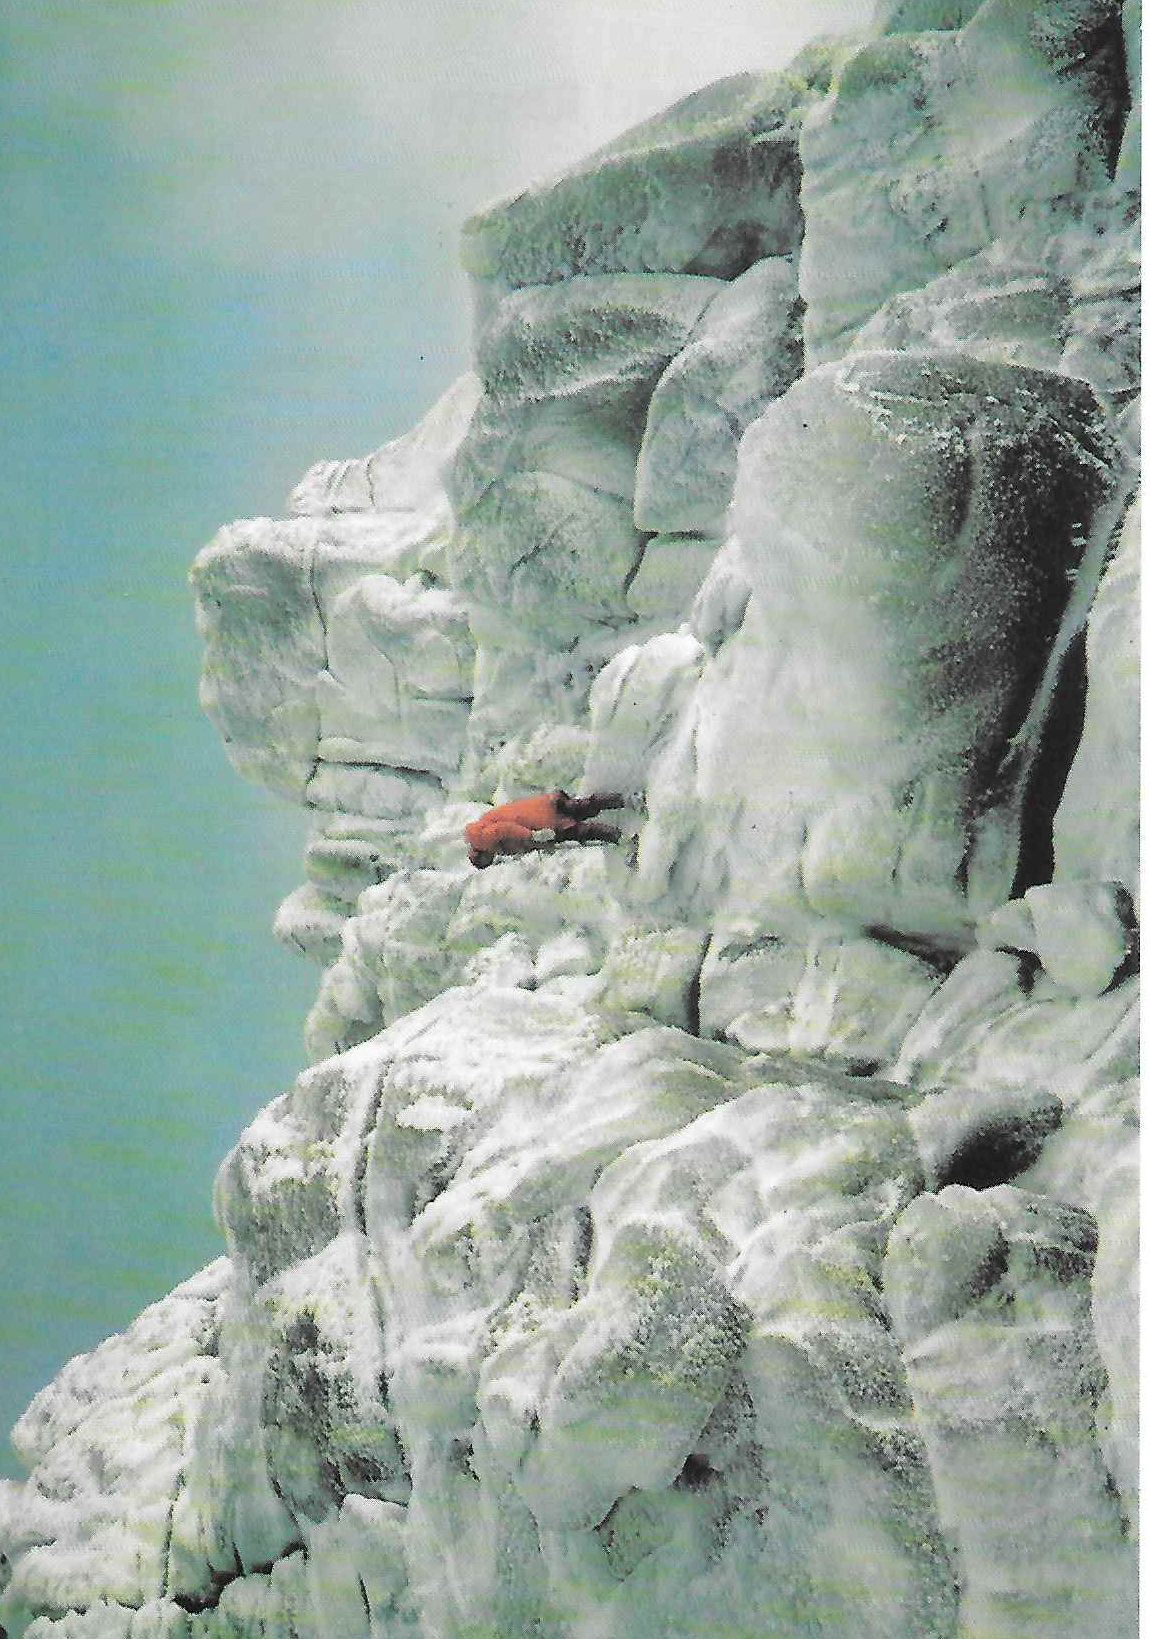
\includegraphics[width=.9\linewidth]{./images/Summit_of_Ben_Avon_Cairngorms.jpg}
\caption{\label{fig:org51fdc4f}
Summit of Ben Avon Cairngorms}
\end{figure}

\chapter{A Three Second Route}
\label{sec:org5aa6145}
\chapterauthor{Marian Birkett}

A summer evening's gritstone climbing   what more could you
ask for? Hilary and I walked up to the "Unconquerable" area of
Stanage to meet various friends. Pippa and Lisa were just
starting  Right Unconquerable   HVS . I had made the mistake of
climbing  Little Unconquerable  once before, a VS overhanging
gritstone crack, so that was out. What was left? Well, that was
it -  Left Unconquerable , E1 5b   a route I'd been eyeing up for
some time.

The short crack which it shares with  Right Unconquerable
leads to a small ledge, then the crack continues steeply to some
overlaps. The next bit, a sort of awkward lay away, is the crux
after that, big holds up the final steep section lead to the top.

I unpacked my sack. I'd just bought some new rock boots,
B3s, only  £25  I can't resist a bargain!  but I hadn't tried them
out yet. Lisa was amazed that I was going to wear them for the
first time on this particular climb. I reasoned that they had to
be better than my Crag Rats and that I needed all the help I
could get. I'd been away and hadn't climbed on gritstone for some
weeks.

I started badly. I took at least ten goes to climb the first
short  supposedly straightforward  crack. The boots were
incredibly uncomfortable: why do they always feel alright when
walking round the shop? I started up the steep crack, putting
lots of runners in   I'd got far too much gear as usual, so I
might as well get rid of it. By the time I'd reached the overlap
my arms were screaming   I spent a while getting Friends in the
horizontal crack and then my ethical stance lowered somewhat.

"Can you hold me on the rope, Hilary?"

Oh, the relief of being able to let go with my hands! A good
while later, I'd rehearsed in my mind the moves I needed to make
and psyched myself up ready to go.

"OK Hilary, I'll have another go!"

First get the feet in the longitudinal crack   another small
ledge a bit higher, lay away with the left hand , reach up with
the right   not much of a hold that! Now, keep going   another
couple of moves and I'd reached the big jug with my left hand
marvellous, I'd done it. Or had I? I just needed to get  my left
foot up on that hold and it was still some inches away. My hands
wouldn't work: I was staring at my fingers willing them to stay
there but I saw them slowly uncurling. Whoosh! Suddenly I was
twenty feet lower down, hanging upside down, staring stupidly at
Hilary. She had been sitting down and had been lifted off her
feet as I fell. I felt surprisingly little jolting  it was the
first time I'd fallen when leading unless you count a fall from
about eight feet up a route when my landing was cushioned by my
second's head . I swung the right way up, pulled myself back to
the steep crack, clipped into a runner and hung there to take the
weight off Hilary and to have a rest. So near and yet \ldots{}

The others were hoping I'd give up. The midges were biting
and the pubs were open. No chance! I knew I could do it. I'd done
the hard move. I'd just have to do it quicker so I didn't run out
of strength next time.

By this time Pippa had completed  Right Unconquerable  and so
had Lisa. They were getting ready to go. Pippa, thinking that
Hilary would like a rest after belaying me for about an hour,
took over from her. I struggled back up the crack to the overlap.
I was trying to conserve energy as my hope of a clean ascent was
now long gone and I rested often. At the overlap I rested a good
while on a runner, long enough to thoroughly bore Pippa, who now
handed over to Lisa   my third second on this one route.

Realising it was getting dark and that the pubs would soon
be shut, I gathered my energies for a final assault. Where were
those hand holds? There's the jug! Now, fingers, STAY WHERE
YOU'RE PUT this time. Will my foot reach that hold? Yes! Made it!

I collapsed, puffing and panting, above the crux.
Encouraging noises floated up from below. Just the last bit now.
Let's get a runner in   don't want to do that again. Suddenly,
there I was at the top, a slight breeze trying to blow away the
midges. Up came Hilary and Lisa, congratulating me. My first E1
on grit. Maybe I'll do one properly some day.
\begin{figure}[htb]
\centering
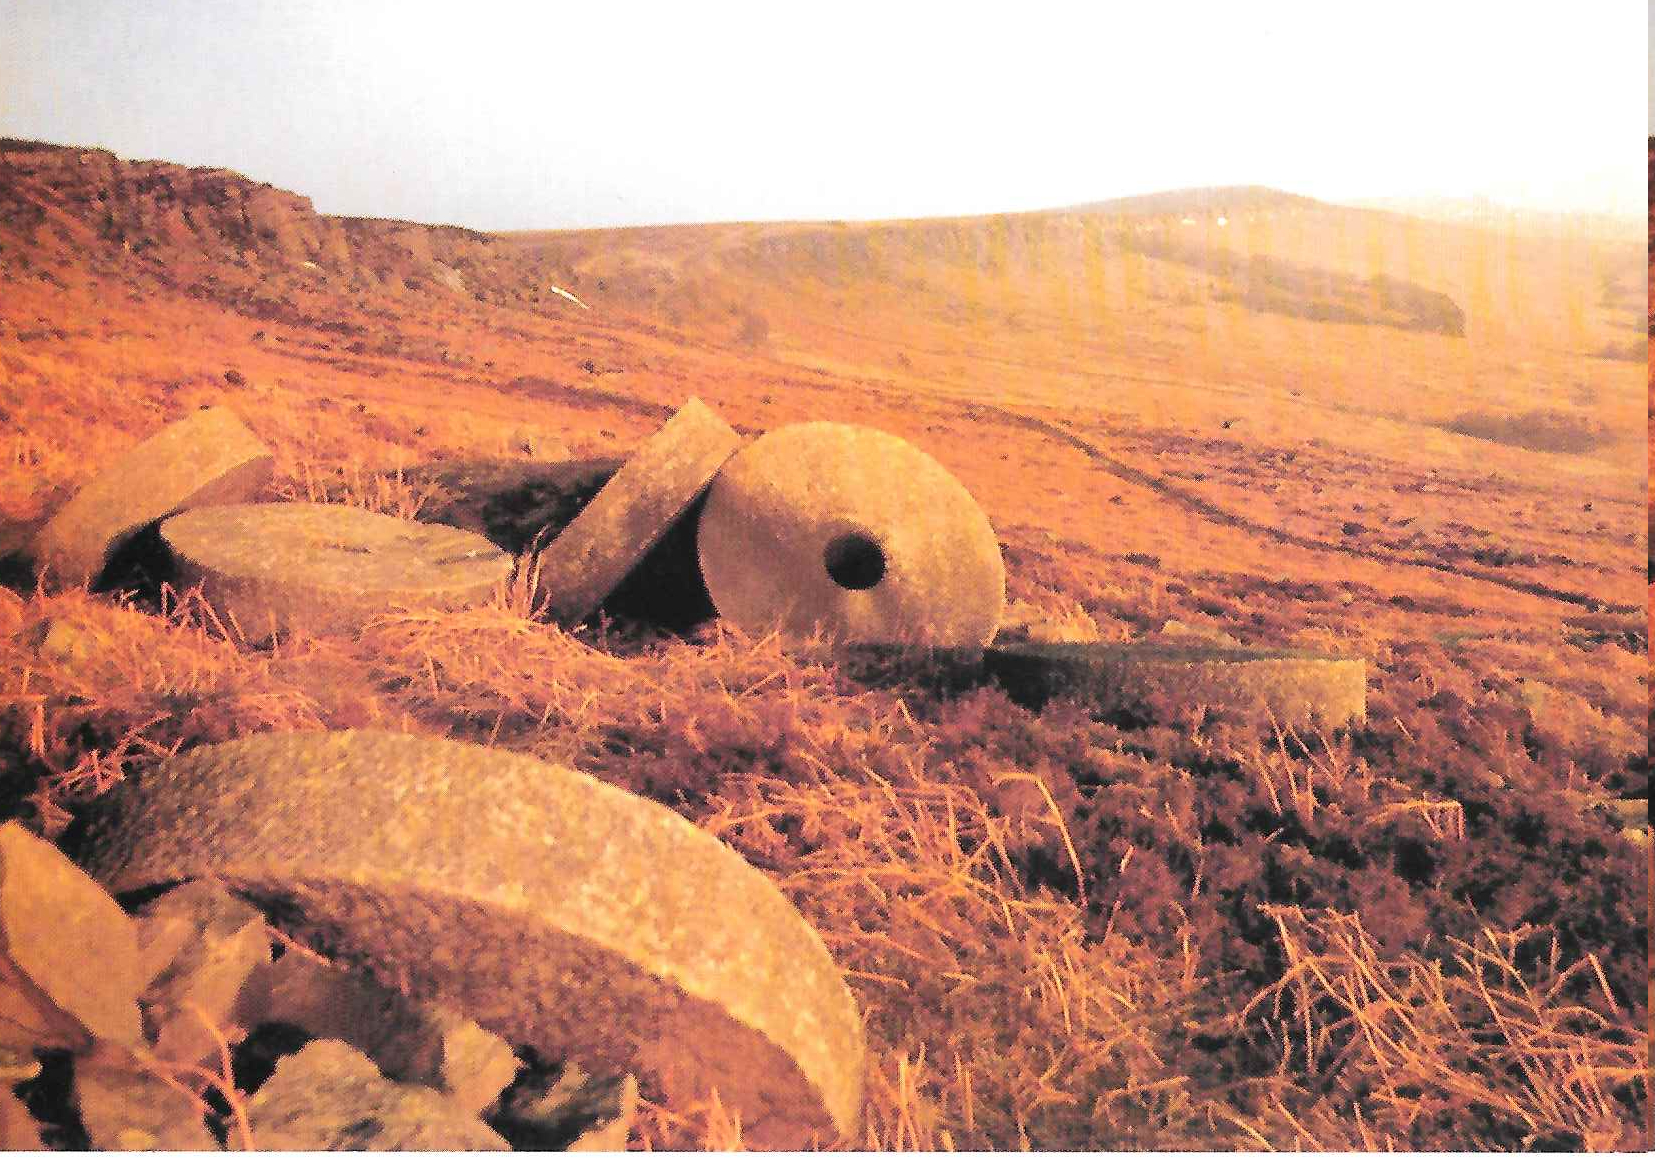
\includegraphics[width=.9\linewidth]{./images/Autumn_Stanage.jpg}
\caption{\label{fig:orgb0741e8}
Autumn at Stanage}
\end{figure}

\begin{figure}[htb]
\centering
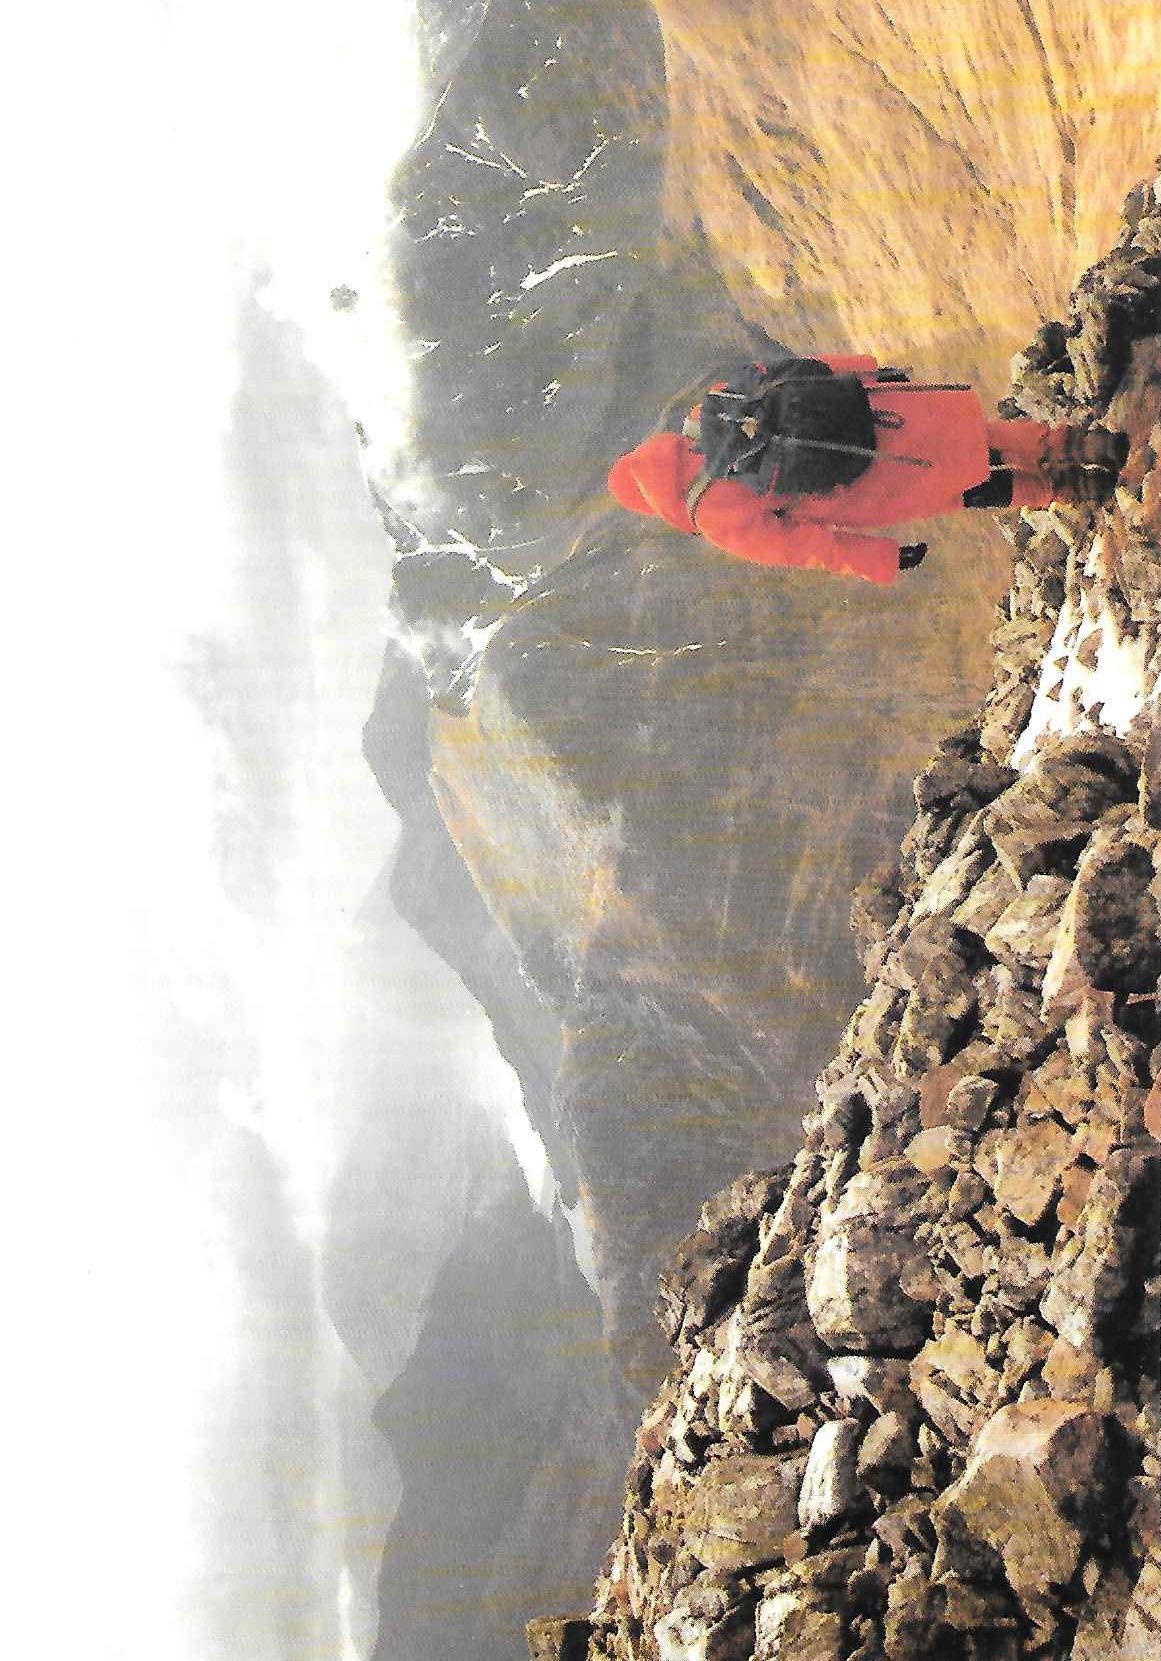
\includegraphics[width=.9\linewidth]{./images/On_the_Mamore_Ridge.jpg}
\caption{\label{fig:org07f2fd2}
On The Mamore Ridge}
\end{figure}

\chapter{The Munros a Personal Pilgrimage}
\label{sec:orgdf52995}
\chapterauthor{Mike Jackson}

A number of small groups tackled the last few hundred feet
of ascent over slabby rock pavements and areas of stone and
gravel. The bare slopes held pockets of wind blown snow and the
clumps of grass were encased in frost and rime, forming masses of
exquisite white patterns. Eyes strained through the dense mist
for the elusive summit until we finally arrived at the ice encrusted cairn.
A full bottle of a favourite liqueur whisky was
produced   with matching glasses, a real touch of class that!
and the congratulations of everyone present were eagerly offered
and gladly received. For me it was the culmination of a personal
pilgrimage which had started long before\ldots{}

My family had settled in Sheffield in 1947 and it was in the
wild moorlands and beautiful countryside of the delightful Peak
District that the foundation of my love for the hills was well
and truly laid. I first visited Scotland as a student in 1957 and
my first Scottish ascent was of Cairngorm from a wild and stormy
campsite at the head of Loch Avon. The vast scale and magnificent
wilderness of the Cairngorms made a deep and lasting impression
on me but, apart from a solitary trip to Glen Nevis, eleven years
passed by before I joined the CMC and at last found the
opportunity of visiting Scotland on a regular basis.

The Club had been founded in 1967 by Alec Barclay, an
expatriate Scotsman whose apparently unlimited energy and
enthusiasm soon attracted a keen following and ensured the Club
its future success. Vital features in the attraction of the Club
were the emphasis on individual inclination and achievement and
the complete absence of unnecessary regimentation. Mountaineering
with the Club was always enjoyed with the greatest of relish and
the away meets in particular were awaited with keen anticipation,
each one an adventure for those fortunate enough to be able to
take part.

My first Scottish club meet was to Lagangarbh in Glencoe in
1969 when the only carload of enthusiasts also included Alec
himself  first Hon. Secretary , Colin Mackie  first President ,
Chris Taylor  first Treasurer , Kate Peek  still a member twenty
years later . The highlight was a thrilling traverse of the
spectacular Aonach Eagach ridge in superb conditions of sunshine
and mist during the only all too brief clear interlude in a
weekend of torrential rain.

The first meet I organized myself was to Lochnagar the
following October and in the years to come I attended every one
of fourteen consecutive July meets in Glencoe and enjoyed visits
to many different areas of Scotland at all seasons, particularly
to the Cairngorms in the winter snows, establishing a welcome
programme of unfailing interest and excitement.

In 1972, during the Club's first Skye meet and after an
unforgettable day on the Black Cuillin, I discovered at the SMC
hut in Glen Brittle a slim volume which was to transform my hill
walking and result in a sense of commitment and direction I had
not previously experienced. It was, of course, "Munros Tables"
and a quick examination disclosed the enormous range of 3000 foot
summits in Scotland, far more than I had ever contemplated. I
had, it appeared, climbed only twenty three Munros and my
exploration of the Scottish hills had scarcely begun. The thought
of tackling them all fired my imagination and the long trail I
then began to follow was to lead me over the years to endless
hours, days and weeks of inspiration and delight.

A number of CMC members became equally attracted to the
Highlands and the intensity of our weekend forays increased both
in summer and in winter as the years rolled by, with early starts
from Sheffield on Friday morning in order to tackle our chosen
hill during the afternoon after our long journey. We would enjoy
a very full expedition indeed on Saturday and a considerable
outing on Sunday before dashing home in time to start work on
Monday morning. More remote areas provided an excuse or reason
for longer visits using bothies and youth hostels or camping in
the wilds  particularly successful and memorable expeditions
included those to the Far North, Skye, Torridon, the Cairngorms
and even a boat trip to the Western Sea Lochs. My most regular
companion became Jim Thomson whom I first met on an early
Cairngorm meet and who eventually completed his Munros in 1983 on
the very day of his seventy third birthday when I had the great
pleasure of standing with him on a remote summit in the Rough
Bounds of Knoydart. My sons Andrew, John and Christopher have
also enjoyed the hills and their arrival on the Scottish scene
brought me added joy.

In the course of climbing the Munros, an appreciation grows
of the great variety of Scottish hill scenery ranging from the
massive grandeur of the Cairngorms to the incomparable
excitements of the Skye Cuillin and from the sea views and
enchanting situations of Western Highland peaks to the dramatic
individual hills and ranges of the Northern Highlands. The quest
for the Munros takes one the length and breadth of the land and
ensures that many a fine hill is enjoyed that might not otherwise
have been attempted. The contrasts of the seasons   the wonderful
clarity of the springtime views, the sunshine, rain and greenery
of high summer, the glorious autumn colours and the superb
snowscapes of winter   all add to the unfailing interest and
variety of experience.

The planning of an expedition, the commitment to set off for
the summits in all weathers except the downright impossible, the
determination to pit one's strengths  and weaknesses  against the
demands of the task in hand  even on days of rain, storm and
blizzard that can on occasion make hill walking a taxing
exercise  all contribute to the challenge. The discomforts and
occasional hardships are invariably amply compensated by the
beauty of outstanding scenery and the majesty of the natural
world, the heady excitements of ridge and crag, the abundant and
precious wildlife and the companionship of good friends.

My ambition was to end my personal Munro trail in the
Cairngorms where I had climbed my first Highland hill thirty
years earlier   this grand area of high wilderness, long
distances and far horizons. And so it was, on a dark day in
October 1987, that I found myself on that bleak summit nine miles
from the nearest road, sharing a very special occasion with many
of the friends and fellow members of the CMC with whom I had
enjoyed so many wonderful hill days. I was particularly delighted
that my dear friend Jim and my youngest son Christopher were both
present   an age range of no less than sixty four years! I had
hoped for bright sunshine and great views but it was perhaps
appropriate that we had chosen an autumn day requiring some
measure of hillcraft.

After approaching this moment with ambivalent feelings, the
end of my long pilgrimage proved in the event to be yet one more
heartwarming experience after so many enjoyed on the hills over
the years   experiences which in relation to the Highlands could
be renewed a hundred times without fear of duplication. I have
had the good fortune of sharing my endeavours with proven friends
who also love these marvellous hills  they are too numerous to
mention individually but they know who they are and that they
enjoy my admiration and my gratitude: my heartfelt thanks to all
such friends and in particular to my fellow members of the CMC.

\chapter{Sentimental Ramblings of an Early Club Member}
\label{sec:org9e5b62b}
\chapterauthor{EKate Fowler or Kate Peek, to many}

The last time I visited The Castle Mountaineering Club
clubroom was in August 1986, during a hectic trip to England to
put our house up for sale, pack belongings, and say farewell to
family and friends. Alan and I had decided to settle in Norway
after an initial two year contract and the reason we'd taken the
temporary appointment in the first place had, I believe, much to
do with the CMC. More than twenty years ago, only a few months
after the Club was founded, I became an official paid up member
and apart from honorary members, I believe Mike Anderson and I
are now the longest standing Club members. From that time on my
love for the hills and wild open spaces grew  hence the prospect
of new hills, combined with months of skiing was too great to
turn down.

My experiences have ranged from early attempts at rock
climbing, being more or less hauled up Diffs on Froggatt, moist
struggles up "The Buachaille" from the warmth and  in those days
squalor of Lagangarbh, suicidal snow ploughs in white outs down
the White Lady on Cairngorm and dirty bog trotting days on
Kinder, to classic climbs in Llanberis, back packing in the
remoter parts of the Scottish Highlands, summer holidays in the
French Alps and now, the thrills and pleasure of Langrenn skiing
over mountains, through forests  and even on the sea in a good
winter , for several months of the year.

I have no claims to great conquests, either on rock or hill.
I've never been one for seeking the highest, fastest or hardest
and my one attempt at outdoor competitiveness was a farce. This
was the first Edale Skyline Race and the late Don Morrison
cajoled me into entering.

"You're fit," he said.

Well, I'd not run anywhere for nearly fifteen years and I
was, in those days, a very heavy smoker! I came in last  OK, many
had dropped out by the wayside  and when I arrived back at Edale,
nearly everyone had packed up and gone home. A voice from the
darkness cried:

"Well done Kate, you've come second in the ladies section."

Now, there were only four to start with and two of those had
dropped out!

My only connection with anything remotely organized on rock
and hill is that I did decide to tackle the Munros: I had in fact
just reached a little over half way with my Munros when we
emigrated to Norway and I haven't completely given up the idea of
finishing them completely one day. Even the ones I tackled were
often attempted in a very come day go day fashion: it was more a
means of being attracted into areas I might not otherwise have
entered.

Any "conquests" have been purely personal. A long, hard day
in the hills has been pleasurable for the hours spent in wild
scenery and possibly wilder weather with CMC members, people I've
felt comfortable with, whose judgement I trust and respect in
difficult situations, and with whom I've relaxed later over a
pint. My rock climbing, by today's standards, has been extremely
humble although in the early days, women climbers were still very
much in the minority and I've received a fair dose of leg pulling
and many strange remarks. I've led the odd VS and a few Severes
but most of the time I've seconded. However, the highlights, to
me, have been days such as the one on Dinas Mot, when I stood at
the foot of  Direct Route , my first long Welsh VS, and shivered in
terror as I watched an International Party of climbers ready for
their ascents on various routes. They all seemed to know what
they were about. They were all clad in smart stretchy clothes and
had chalk bags and confidence and I was still behind the times
with thick breeches and sweaty hands. However, once my feet left
terra firma all fear disappeared and on the last pitch I belayed,
sat in the sun and chatted to other CMC members on a nearby
route, content that I'd climbed the route well and enjoyed every
moment.

My participation as a member of the CMC has, as for many
others no doubt, altered over the years. In the early days of the
Club I thrived on doing anything "en masse". Climbing was rarely
a quiet affair between leader and second, but more an invasion of
one climb by as many people as possible. I remember vividly
 Browns Eliminate  on Froggatt being peppered with struggling
bodies  mine being one , all being top roped at the same time. It
became like a child's puzzle, trying to trace back the rope to
"which leader?" We even drove in convoy on away meets to
Scotland! Safety in numbers? Would the natives attack us? Over
the years I became more solitary and anti social in my forays
into the hills, although I still enjoyed the getting together
with Club members at the end of the day. And now   well, not much
chance of joining club meets very often from this distance, but I
do have fantastic memories of past ones.

I would have liked to think that my five year old son
Alisdair would have been able to grow up with the CMC. Alan and I
took him onto Curbar Edge the very day he came out of the
hospital where he was born and I said to him:

"This is air, these are rocks and that lump over there is
Win Hill, I hope you'll learn to love 'em!"

We had taken him on several Club meets before, sadly, we had
to leave the Sheffield area. However, those first impressions
appear to have stuck and he is now knowledgeable on nature and
accepts walking and the hills as a normal part of life.

Over the years, through the CMC, I've made some very good
friends and now one of the greatest pleasures for Alan, Alisdair
and myself is to welcome those friends here to Norway to enjoy
our fantastic scenery and the many varied outdoor activities.
Plus sharing a lot of nostalgia over the duty frees they bring!

Well, as I said at the beginning, my last visit to the
clubroom was almost two years ago. There were many new faces but
the atmosphere of a thriving and friendly CMC has little changed.
I hope that all newer members and older ones alike can look back,
like me, after twenty years of CMC membership and enjoy as many
wonderful memories and as many good friends.
\begin{figure}[htb]
\centering
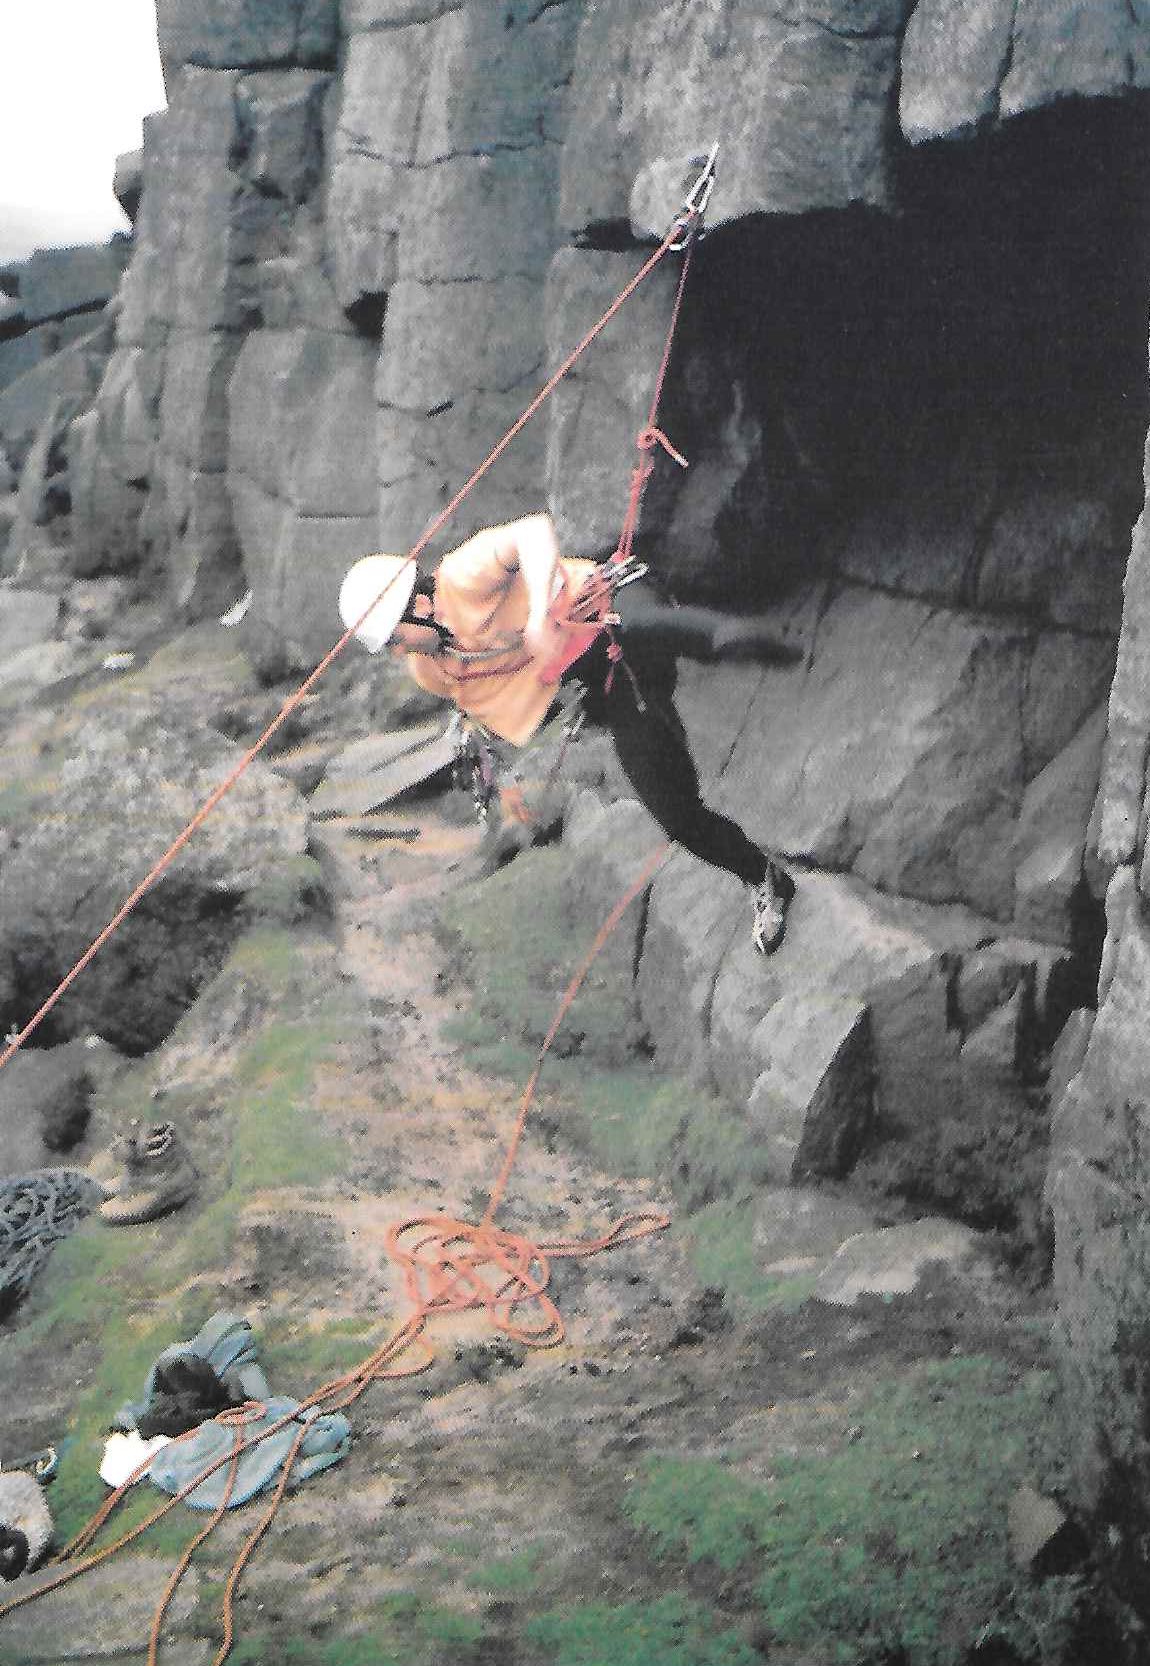
\includegraphics[width=.9\linewidth]{./images/Dave_Dunk_on_Marmoset_Stanage_Edge.jpg}
\caption{\label{fig:org71fc003}
Dave Dunk on Marmoset Stanage Edge}
\end{figure}

\chapter{Grit Biter}
\label{sec:org876111d}
\chapterauthor{Frank Mellor}


In the summer of '86 siege tactics were employed on a
twenty foot route at Stanage. Although the attempt was
unsuccessful the style in which it was made inspired this poetic
gem.

I watched a wind blown figure
Below a roof of rock,
A holey orange tee shirt
And a badly darned left sock.

His right leg and his forearms
Are quivering fit to bust,
In another two short seconds
He will surely Bite the Dust!

His Springer spaniel and his wife
Both watch, devoid of hope,
For the sixteenth time that afternoon
He sags onto the rope.

"I'll give it one last try," he says,
The chance must not be missed
And so into that loathsome crack
He jams his bleeding fist.

A few choice words he mutters
And wears determined frown,
But odd EBs kick at the air
And he hangs there, upside down!

The watchers roar in sheer delight
To see this latest antic,
I fear this beastly little route
Will drive our hero frantic.
He will return once more he vows
To do it in the wet!
Perhaps, with helmet back to front,
He'll catch you Marmoset.

\chapter{Some Thoughts on Mountaineering}
\label{sec:org8acf190}
\chapterauthor{Alec Barclay}

Why climb mountains? This is a question which has been asked
so many times over and is one to which it is difficult to give a
satisfactory answer. The question is usually posed in such a way
that a dramatic answer is expected  but this need not necessarily
be the case: mountaineers climb mountains for different reasons
and these reasons can change each time an ascent is made. One
reason may be the basic primeval urge to pit one's resources
against what nature has to offer, but it might equally well be an
escape from one's normal environment in order to release pent up
pressures.

Whatever the reason, mountains are Nature's answer to these
pressures and to involve oneself completely in their presence is
an experience from which one returns refreshed and better able
spiritually, physically and mentally to face up to life as we
experience it.

My own involvement goes back to childhood days when a tree
with plenty of branches presented a challenge and  small outcrops
of rock provided an outlet for youthful zeal. The war years
afforded the opportunity to climb abroad  in The Lebanon,
Australia and New Guinea  but since then all my climbing has been
in Scotland, The Lake District, North Wales and The Peak
District.

The late fifties marked for me a late self proving era when
in the company of good friends I spent many weekends on the crags
of Glencoe and Ben Nevis, rock climbing in summer and snow and
ice climbing in winter. My companions of those happy days went on
to to greater things and tragically many are now gone, having
died on the very hills they loved so much.

I have remained actively involved in climbing and skiing
in my time I have founded two mountaineering clubs, one in
Sheffield and the other in Livingston near Edinburgh   but no
longer do I have the urge to tackle the impossible. However, one
must guard against the ever present urge to modify difficulty.
Organized society habitually seeks the smoothest way. With
mechanization and labour saving devices, life has become so
smooth that some of us seek a necessary corrective in grappling
with rough undisciplined crags. For me, climbing has always
seemed to embody some immutable principle: something stable in a
changing world.

Many people look upon mountaineering as a dangerous pastime
and believe that its devotees take their lives in their hands
whenever they go climbing. But the average mountaineer probably
does not incur more danger to life than a man who heartily goes
in for any one of half a dozen favourite pastimes. Admittedly,
there is an element of danger in serious climbing, but it is, or
should be, a calculated risk. In climbing snow or rocks,
familiarity does not breed contempt, but it does enable one to
see things in their true proportions, to appreciate real dangers
and to ignore imaginary ones, and particularly to gauge just what
one can achieve personally. Climbing is a test of nerve, skill,
endurance and judgement  the climber should know his limitations
and how far he can risk a move in safety. In proportion to the
large numbers of climbers active on the hills, the loss of life
by accident is in fact infinitesimal.

"A man is immortal 'til his work is done" and if he is ready
for the call when it comes, he may just as well perish on a
mountainside as be bowled over by a car, or succumb to fatty
degeneration of the heart.

In Ruskin's beautiful words:

"Mountains are the great cathedrals of the earth, with their
gates of rock, pavements of cloud, choirs of stream and stone,
altars of snow and vaults of purple traversed by the continual
stars."
\begin{figure}[htb]
\centering
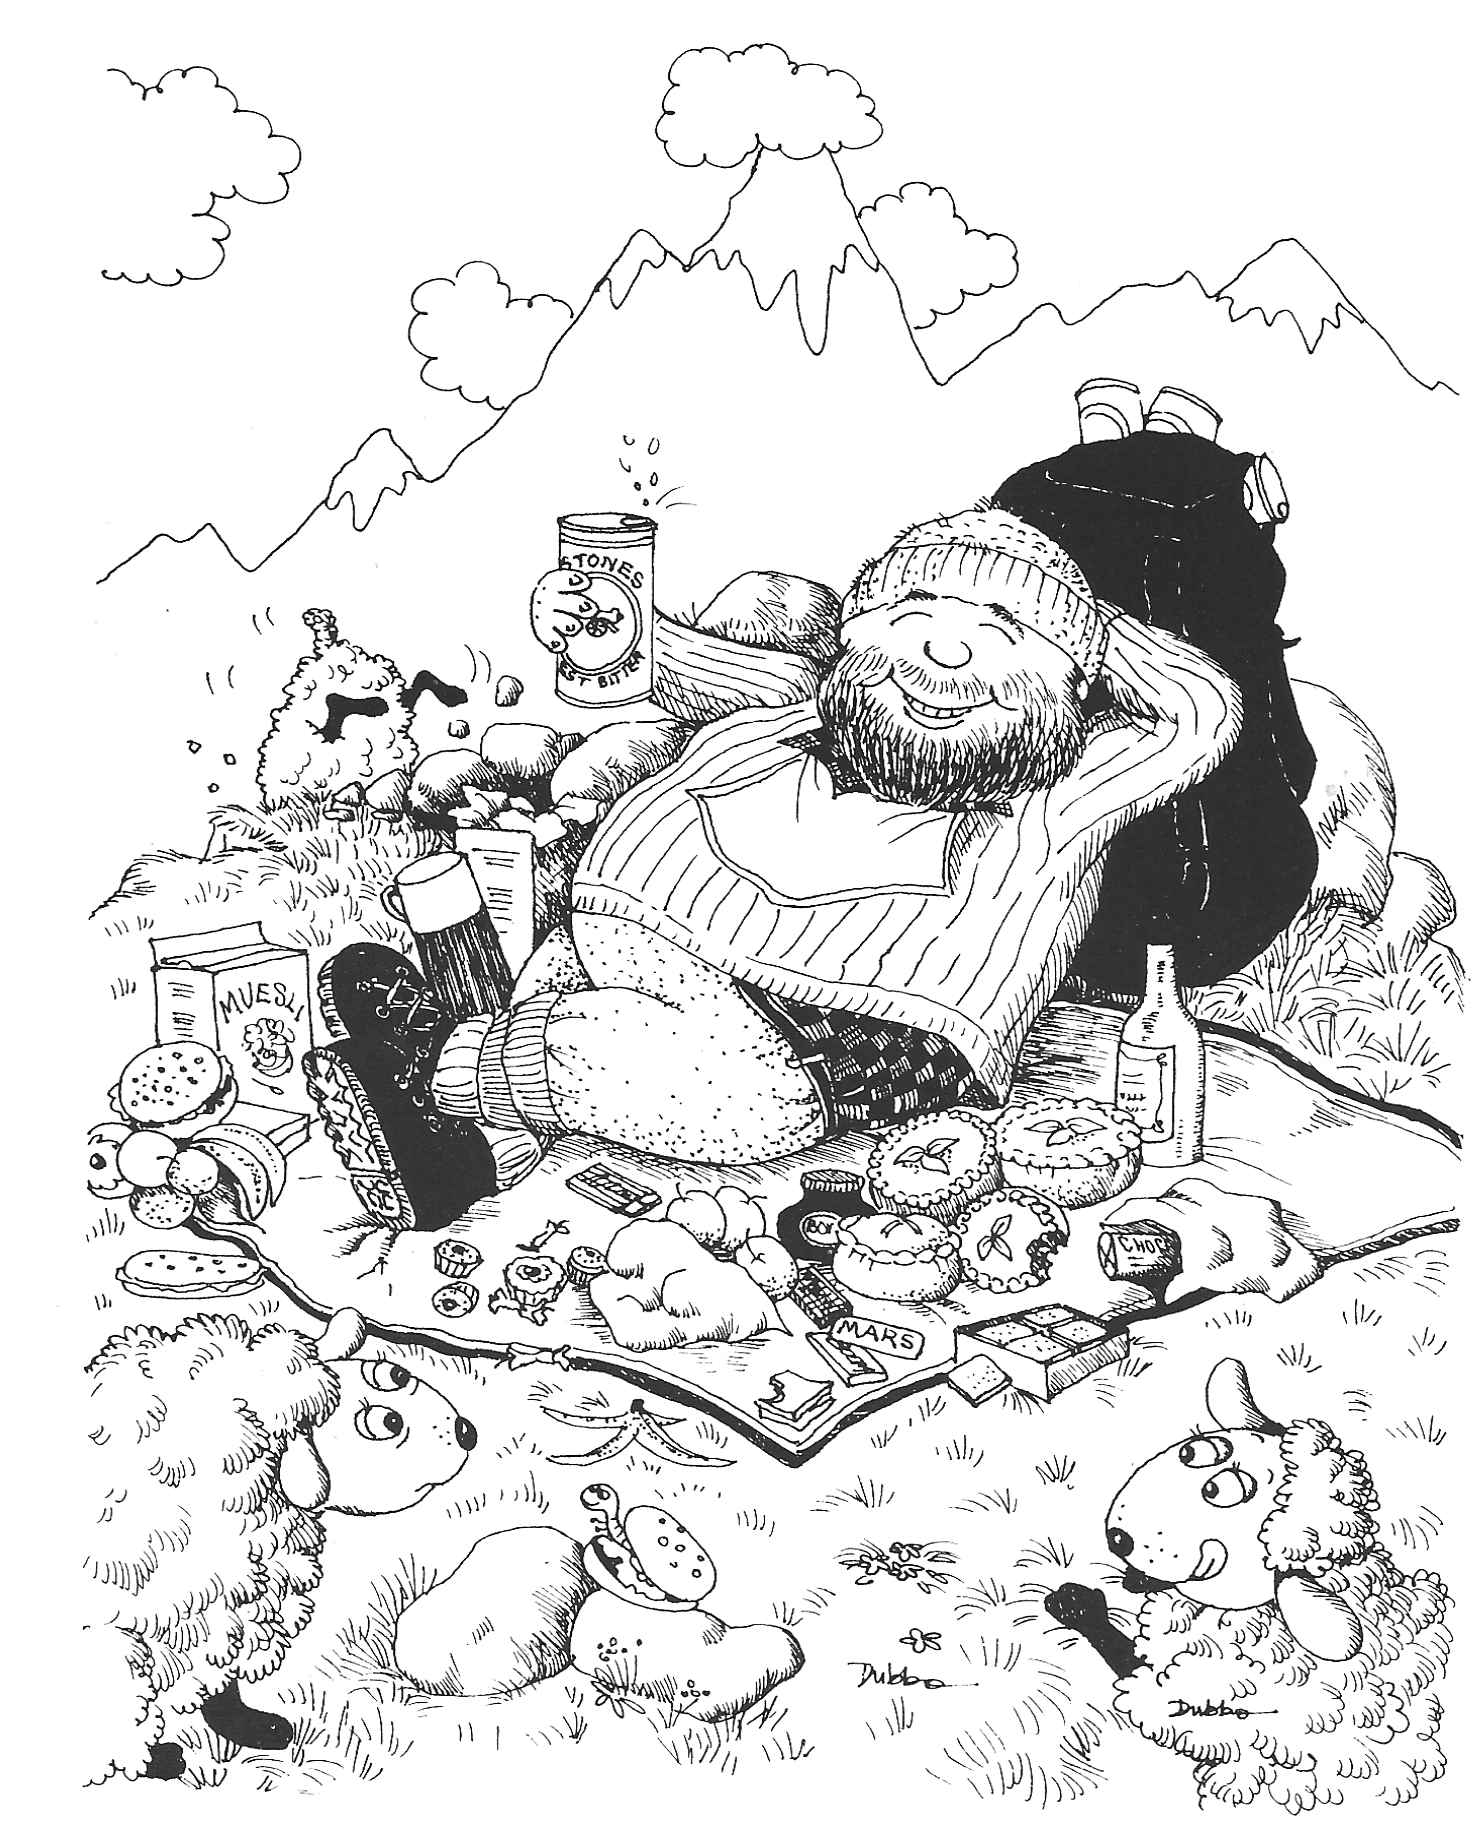
\includegraphics[width=.9\linewidth]{./images/Cartoon_16.jpg}
\caption{\label{fig:orge479946}
Some Thoughts on Mountaineering}
\end{figure}
\end{document}
